%%% DOCUMENTCLASS is KOMA-Script scrbook with documentation in http://mirrors.ctan.org/macros/latex/contrib/koma-script/doc/scrguide.pdf
\documentclass[draft=false,titlepage=firstiscover,bibliography=totocnumbered,index=totocnumbered,11pt,headings=openany]{scrbook}
%
%%%%%%%%%%%%%%%%%%%%%%%%%%%%%%%%%%%%
% PACKAGES
\usepackage[utf8]{inputenc}
\usepackage[T1]{fontenc}
\usepackage{textcomp}
\usepackage{hyperxmp}
\usepackage{amsmath}
\usepackage{scrhack}
\usepackage{listings}
\usepackage[american]{isodate}
\usepackage{multirow}
\usepackage{graphicx}
\usepackage{epstopdf}
% Setup for eps-to-pdf to comply with PDF/A
\epstopdfsetup{
program@epstopdf=epstopdf
--pdf-version 1.4
}
%\edef\hash{\string#}
%\epstopdfsetup{
% program@epstopdf=epstopdf
%   --gsopts "-dPDFA -sProcessColorModel\hash DeviceCMYK
%     -sPDFACompatibilityPolicy\hash 1
%     -dCompatibilityLevel\hash 1.4",
%}
%–––––––––––––––––––––––––––––––––––
\usepackage{setspace}%
\usepackage[english,german]{babel}
\usepackage{hologo}
\usepackage[numbers,sort&compress]{natbib}
\usepackage{bibentry}
\usepackage{makeidx}
\usepackage{titlepage}
\usepackage[type={CC},modifier={by},version={4.0},imagemodifier={-eu},lang={english}]{doclicense}
\makeindex
\usepackage{hyperref}
%___________________________________
%
% hyper setup for meta-data
\hypersetup{%
		%pdfTeX,
		%shared hyperref and hyperxmp data
		baseurl={https://github.com/Maderthaner/Thesis/blob/master/main.pdf},
		pdfauthor={Maximilian Jakob Bucher},
		pdfkeywords={LCLS, FEL, Cluster},
		pdflang={en},
		%pdfproducer={pdftex},
		pdfcreator={LaTeX with hyperref package},
		pdfsubject={Free electron laser science},
		pdftitle={Ultrafast Dynamics of Nanoparticles in Highly Intense X-Ray Pulses},
		%hyperref specific options
		%bookmarks=true,         % show bookmarks bar?
		bookmarksnumbered=true,
    	unicode=true,          	% non-Latin characters in Acrobatӳ bookmarks
	  	pdftoolbar=true,        % show Acrobatӳ toolbar?
	  	pdfmenubar=true,        % show Acrobatӳ menu?
	  	pdffitwindow=false,     % window fit to page when opened
	  	pdfstartview={FitH},    % fits the width of the page to the window
	  	pdfnewwindow=true,      % links in new window
	  	colorlinks=false,       % false: boxed links; true: colored links
	  	linkcolor=red,          % color of internal links
	  	citecolor=blue,        	% color of links to bibliography
	  	filecolor=blue,      	% color of file links
	  	urlcolor=blue           % color of external links
		%hyperxmp specific options
		pdfaconformance=B,
		%pdfapart=1,
		pdfauthortitle={Master of Science},
		pdfcaptionwriter={Maximilian Jakob Bucher},
		pdfcontactaddress={Technische Universität Berlin, Universitätsbibliothek, Dissertationsstelle, Fasanenstr. 88},
		pdfcontactcity={Berlin},
		pdfcontactcountry={Germany},
		pdfcontactemail={dissertationen@ub.tu-berlin.de},
		pdfcontactphone={+49(030)314-76129},
		pdfcontactpostcode={10623},
		pdfcontactregion={Berlin},
		%pdfdate={2016},
		pdfcontacturl={http://www.ub.tu-berlin.de/en/university-press-and-theses/dissertation-office/},
		pdfcopyright={This work by Maximilian J. Bucher is licensed under the Creative Commons Attribution 4.0 International License.},
		pdflicenseurl={http://creativecommons.org/licenses/by/4.0/},
		pdfmetalang={en-US}
}
\usepackage[a-1b]{pdfx}
%___________________________________
%
%
\begin{document}
\nobibliography*
\onehalfspacing
\selectlanguage{english}
\pagenumbering{alph}
%\maketitle
%
% Need titlepage package, see here: http://www.komascript.de/titlepage
\begin{fullsizetitle}
\vspace{40mm}
\begin{center}
%
%\hspace{0mm} \vspace{0mm}\hspace{0mm}\\%
{\LARGE \textbf{Ultrafast Dynamics of Nanoparticles\\in Highly Intense X-Ray Pulses\vspace{20mm}\\}}%Coincident imaging and ion spectroscopy\\of single large xenon clusters\\in high intense soft x-ray pulses\vspace{25mm}\\}}
{\large%
vorgelegt von
\vspace{4mm}\\
Master of Science}%
\vspace{2mm}\\
%
{\Large Maximilian Jakob Bucher}
\vspace{4mm}\\
%
{\large geb. in Frankfurt am Main} %
\vspace{20mm}
\\
%
{\large %
von der Fakultät II - Mathematik und Naturwissenschaften
\vspace{1mm}\\
der Technischen Universität Berlin
\vspace{1mm}\\
zur Erlangung des akademischen Grades
%
\vspace{7.5mm}
\\
%
Doktor der Naturwissenschaften
\vspace{1mm}\\
- Dr. rer. nat. -
%
\vspace{7.5mm}
\\
%
%
%%% vorgelegte Dissertation zur Eröffnung des Promotionsverfahrens
%vorgelegte Dissertation
%%% genehmigte Dissertation nach abschluss der Promotionsprüfung / wissenschaftlichen Aussprache
genehmigte Dissertation
%
\vspace{10mm}}
\\
\end{center}
%
{\large%
\hspace{22mm}Promotionsausschuss:
%
%
\begin{tabbing}
%
\hspace{22mm}\= Vorsitzender:\hspace{20mm} \= Prof. Dr. Mario Dähne \\
\>Berichter/Gutachter: \> Prof. Dr. Thomas Möller \\
\>Berichter/Gutachter: \> Prof. Dr. Christoph Bostedt \\
\>Berichter/Gutachter: \> Priv. Doz. Dr. Tim Laarmann
%
\end{tabbing}
%
\leavevmode
\hspace{22mm}
%%% Tag der wissenschaftlichen Aussprache auskommentieren, wenn unbekannt / noch nicht bestanden.
Tag der wissenschaftlichen Aussprache: 12. Dezember 2017
}
%
\begin{center}
%
\vspace{20mm}
%
{\large %
Berlin 2017}
%
\end{center}
%
\end{fullsizetitle}
%
%
\pagenumbering{gobble}
\begin{flushleft}
{\Large M.Sc. Maximilian Jakob Bucher}\\
\footnotesize{Argonne National Laboratory\\
Chemical Sciences and Engineering Division\\
Argonne, IL 60439, United States\\
\vspace{0.5cm}

SLAC National Accelerator Laboratory\\
Linac Coherent Light Source\\
Menlo Park, CA 94025, United States
\vspace{0.5cm}

Technische Universit{\"a}t Berlin\\
Institut f{\"u}r Optik und Atomare Physik\\
10623 Berlin, Germany
\vspace{0.5cm}

E-Mail: \href{mailto:max@max-bucher.de}{\nolinkurl{max@max-bucher.de} }\\
Web: \url{https://www.max-bucher.de}}
\end{flushleft}
\vspace{10.5cm}
\doclicenseThis
More information can be found under\\
\url{\doclicenseURL}
%This work by Maximilian J. Bucher is licensed under the Creative Commons Attribution 4.0 International License.
%\null\newpage						% ENABLE THIS FOR PRINT
\pagenumbering{roman}
%\part*{blabla}
\section*{Abstract}\label{ch:abstract}
With the advent of lightsources of the fourth generation, such as the X-ray free electron laser (XFEL) the Linac Coherent Light Source (LCLS), structural studies on non-repetitive and non-reproducible nanoparticles such as single biomolecules appear imminent. A key challenge to increasing the resolution of single particle imaging is radiation damage. Only a sound understanding of the underlying damage processes, such as the nanoplasma formation, can overcome this challenge and will ultimately lead to higher resolutions. Sacrificial tamper layers have been proposed to slow X-ray sample damage but this has not been shown experimentally using nanoparticles and diffractive imaging.\\[0.5\baselineskip]
%
This thesis investigates the nanoplasma formation and expansion in superfluid He-, bulk Xe- and mixed HeXe-clusters using an ultrafast, XFEL accelerator-based X-ray pump--X-ray probe technique. A first X-ray pulse triggers the nanoplasma evolution in the sample at intensities of \SI{\sim e17}{\watt\per\square\centi\meter}, and a second X-ray pulse probes the system at a later time, $\Delta t$, at power densities of \SI{\sim e18}{\watt\per\square\centi\meter}. The delay $\Delta t$ is varied between \SIrange{0}{800}{\femto\second}. The probe-pulse creates a diffraction image of the \SIrange{\sim 30}{\sim 1000}{\nano\meter} sized objects and coincidentally ions are captured via time-of-flight (TOF) mass spectroscopy. He- and Xe-clusters are generated through a supersonic gas expansion into a vacuum. Mixed HeXe-clusters are created when He-droplets pick up Xe-atoms in a doping unit. The experiment was performed at the AMO instrument at the LCLS using the LAMP end-station. The LAMP end-station was partly designed, built, and operated as part of this work.\\[0.5\baselineskip]
%
The study reveals single-shot images of Xe-, He- and HeXe-clusters that undergo the nanoplasma formation. The reconstruction of a \SI{\sim 25}{\nano\meter} radius Xe-cluster with \SI{\sim 6}{\nano\meter} resolution is shown. A large-scale structural analysis of the size and number of scatterers in Xe-clusters show rapidly expanding nanoparticles. Expansion speeds and electron temperatures of the nanoplasma are derived. Reconstructions and 2D computer models of few-hundred nanometer radius HeXe-clusters shows that the doped Xe-atoms arrange in small clusters of a plum-pudding type. The He-droplet acts thereby as a sacrificial layer and the Xe-clusters as sample. TOF spectroscopy reveals charge transfer ionization in HeXe-cluster that reduce the electronic damage of Xe-clusters by sacrificing the He-tamper layers. Diffraction images and 2D computer models of HeXe-clusters shows structural damage in the He-droplet, while the Xe-clusters do not exhibit structural damage up to \SI{800}{\femto\second} after the pump-pulse. As a measure of the effectiveness of the sacrificial layer, radiation damage of pristine He- and Xe-clusters are compared to HeXe-clusters.
%
%
%
%
%\section*{Kurzfassung}
\begin{otherlanguage}{german}
Mit der Entwicklung von Freie-Elektronen-Lasern im Röntgen Wellenlängenbereich, wie der \textit{Linac Coherent Light Source} (LCLS), sind strukturelle Studien an Nanopartikeln möglich. Eine Herausforderung bei diesen Studien mit höchst intensiven Röntgenpulsen ist die Beschädigung der Nanopartikel, da dies die Auflösung limitiert. Nur ein fundiertes Verständnis der Strahlungsschadenprozesse, wie die Nanoplasma Expansion, kann die Auflösung verbessern. Weiterhin wurde vorgeschlagen, dass eine Schutzhülle die Nanoplasma-Expansion von Nanopartikeln verlangsamen können.\\[0.4\baselineskip]
%
Diese Arbeit untersucht die Nanoplasma-Transformation und -Expansion in nanometergroßen He-, Xe- und HeXe-cluster, wobei HeXe-cluster ein Modellsystem sind, um den Nutzen von Schutzhüllen zu untersuchen. Die Nanopartikel werden durch eine Überschall Expansion von Gasen ins Vakuum gebildet und werden an der LCLS mit Röntgenstrahlungs-Doppelpulsen zeitaufgelöst untersucht. Hierbei startet ein Pump-Puls die Nanoplasma-Entwicklung mit Intensitäten von \SI{\sim 2e16}{\watt\per\square\centi\meter} und ein Probe-Puls erzeugt Beugungsbilder von dem Nanoplasma zu einem späteren Zeitpunkt $\Delta t$, mit Intensitäten von \SI{\sim 2e17}{\watt\per\square\centi\meter}. $\Delta t$ wird zwischen \SIrange{0}{800}{\femto\second} variiert und die finale Ionenverteilung wird mit einem Flugzeitmassenspektrometer (TOF) gemessen. Das Experiment dieser Arbeit ist in der LAMP Kammer, des AMO Instruments durchgeführt worden. Ein wesentlicher Teil dieser Arbeit war der Bau, die Inbetriebnahme, und die Teilnahme an Design-Diskussionen von der LAMP Kammer.\\[0.4\baselineskip]
%
Die Studie zeigt Einzelschuss Beugungsbilder und TOF Spektren von Xe-, He- und HeXe-clustern mit einer bisher unerreichten Auflösung. So ist beispielsweise die Rekonstruktion eines \SI{\sim25}{\nano\meter} Radius großen Xe-cluster mit \SI{\sim 6}{\nano\meter} Auflösung gezeigt. Die Beugungsbilder und Rekonstruktionen zeigen, wie sich die Nanopartikel zu einem expandierenden Nanoplasma entwickeln. Die Auswertung einiger hundert Einzelschussbeugungsbilder zeigt die Ausdehung der Xe-cluster um etwa \SI{20}{\percent} binnen \SI{800}{\femto\second}. 
%Eine Auswertung einiger hundert Einzelschussbeugungsbilder zeigt, dass der ursprüngliche Xe-Clusterradius um etwa \SI{20}{\percent} im Verlauf von \SI{800}{\femto\second} steigt. Die Expansionsgeschwindigkeit von einem Xe-cluster beträgt \SI{\sim 15250}{\meter\per\second} und die Elektronen Temperatur ist \SI{\sim125}{\electronvolt}.
Rekonstruktionen und 2D Computer Simulationen zeigen, dass sich HeXe-cluster ähnlich eines Rosinenkuchenmodells anordnen, da Xe-Atome in dem He-Tröpfchen zu mehreren kleinen Clustern kondensieren. TOF Spektren zeigen, dass Xe-Cluster kinetische Energie an die Schutzhülle aus Helium transferieren und, dass die Schutzhülle als Elektronenreservoir für die Xe-cluster dient. Die Beugungsbilder der HeXe-cluster zeigen, dass Xe-cluster in den ersten \SI{800}{\femto\second} nicht messbar expandieren, während die He-Schutzhülle einer Nanoplasma-Expansion unterliegt. Abschließend wird die Nanoplasma-Expansion von reinen Xe- und He-Clustern, sowie gemischten HeXe-clustern miteinander verglichen.
\end{otherlanguage}		% WORK ON THIS SOON
\tableofcontents
\listoffigures
\listoftables
%\newpage									% ENABLE THIS FOR PRINT
\null\newpage
\pagenumbering{arabic}
\chapter{Introduction}
%Investigating matter with light is one of the most fundamental approaches to study nature. Whether we look at things by eye or use more advanced methods for example using lasers, it is an invaluable tool to understand nature. Through light, we can study the shapes of objects, investigate fundamental particles, study quantum mechanics and so much more. Key aspect in almost any study involving light is it's wavelength. The wavelength of light can make you feel cozy at home with a modern LED light bulb or shroud your home in a blue, uncomfortable haze when you use older light bulbs. At the end of the 19th century, R\"ontgen discovered the then novel X-radiation and quickly realized its impact due to its different wavelength. Soon, he was able to take first medical X-ray images, later X-rays could be used to investigate fundamental aspects of atoms. The success story continues until today, where short wavelength X-rays enables the study of the workhorse in human bodies, namely proteins. The shape of a protein, which is only a few nanometers in size, cannot be seen in a microscope anymore and only X-rays can be used to unravel their shape with sufficient resolution. The shape of a biomolecules is of particular interest because it defines its biological function. The chemical structure of most human biomolecules are fairly similar and affect the function little. Medical drugs often aim to affect biological functions such that the specific shape of a protein becomes very important for drug research and drug design. \\
% R\"ontgen discovered the X-radiation \citep{Roentgen-NP} and quickly realized its impact due to its novel attributes. Soon, he was able to take the first medical X-ray image.
Following the discovery of X-radiation at the end of the 19$^{\text{th}}$ century by R\"ontgen \cite{Roentgen-NP}, X-rays have been used to understand and investigate matter in new ways. Soon after this discovery, X-rays were used to take the first medical image. Later, X-rays led to the understanding of fundamental aspects of atoms \citep{Siegbahn-NP} and crystals \citep{Laue-NP,Bragg-NP}. Today, the success story continues in various fields of science. A large and active scientific field is structural biology \cite{Karplus-NP,Kobilka-NP}. Here, X-rays are being used to study the structure of proteins through crystallography. Proteins are the so-called ``workhorse'' in the human body and the structure of a protein defines its biological function. Unfortunately not all proteins can be grown into large crystals making the molecular structure determination challenging. However, new light sources, namely X-ray free-electron lasers (XFELs) \citep{Ackermann-2007-NPho}, have more and more peak brightness allowing the structure determination of smaller and smaller protein-crystals \citep{Chapman-2011-Nature}.\\[1\baselineskip]
%
The first free-electron laser reaching into the hard X-ray wavelength range was built at Stanford University and is called the Linac Coherent Light Source (LCLS) \citep{Emma-2010-NatPho}. It is a \SI{3.2}{\kilo\meter} long machine that produces X-rays with wavelengths from \SIrange{4.6}{0.1}{\nano\meter}, provides intensities of up to \SI{\sim e21}{\watt\per\square\centi\meter}, and has ultra-short pulses ranging from \SIrange{1}{500}{\femto\second}. Scientists from various disciplines can apply to use this light source for their experiments, which are conducted in several instruments. The Atomic, Molecular, and Optical physics (AMO) instrument \cite{Ferguson-2015-JSR} at the LCLS was the first of seven instruments in operation and has conducted experiments ranging from biological imaging to basic science \citep{Bostedt-2016-RMP}.\\[1\baselineskip]
%
The intense pulses from XFELs open up an entirely new method for biologists, which is the single particle imaging (SPI). With SPI (see Figure \ref{fig:spi-concept}), the shape of single nanoscale samples can be determined through diffractive imaging \citep{Chapman-2006-NatPhys}. First experiments have successfully delivered single-shot diffraction images of biological particles, such as viruses \citep{Seibert-2011-Nature}, and non-biological particles, such as rare-gas clusters \citep{Gomez-2014-Science}. It has been a rapidly developing field that has recently succeeded in visualizing 3D images of nano-objects \citep{Ekeberg-2015-PRL,Barke-2015-NatComm}.\\[2\baselineskip]
%
%All matter irradiated by intense X-ray radiation disintegrates into its atomic components on ultrafast\footnote{Ultrafast timescales are on the order of atto- to nanoseconds.} timescales \citep{Neutze-2000-Nature}. This process is a form of \textit{radiation damage} and is a major challenge for imaging methods with XFEL \citep{Aquila-2015-StrucDyn}.
%So, the underlying principle of diffractive imaging is that intense X-ray pulses diffract from a single macromolecular structure before they destroy it.\\[1\baselineskip]
%
%Imagine now that we expose a nanoparticle to the highly intense X-rays from LCLS. Within the first moment of light-nanoparticle interaction, photons elastically scatter in an angular distribution distinctive to the shape of the particle that we are able measure in 2D. However, the particle will also absorb the rays from the first moment on, which leads to inner atomic-shell vacancies \citep{Young-2010-Nature}. Subsequent processes, such as the \textit{Auger-decay}, occur only a few femtoseconds later and eventually the nanoparticle is transformed into a \textit{nanoplasma}. Several forces will expand the plasma on a femtosecond timescale \citep{Gorkhover-2016-NatPho}. Finally, the nanoplasma disintegrates into its atomic components. The absorption process, which triggers this cascade of events in the nanoparticle, is unavoidable when the particle is exposed to intense X-rays and so is radiation damage in the sample.\\[1\baselineskip]
\begin{figure}
	\centering
		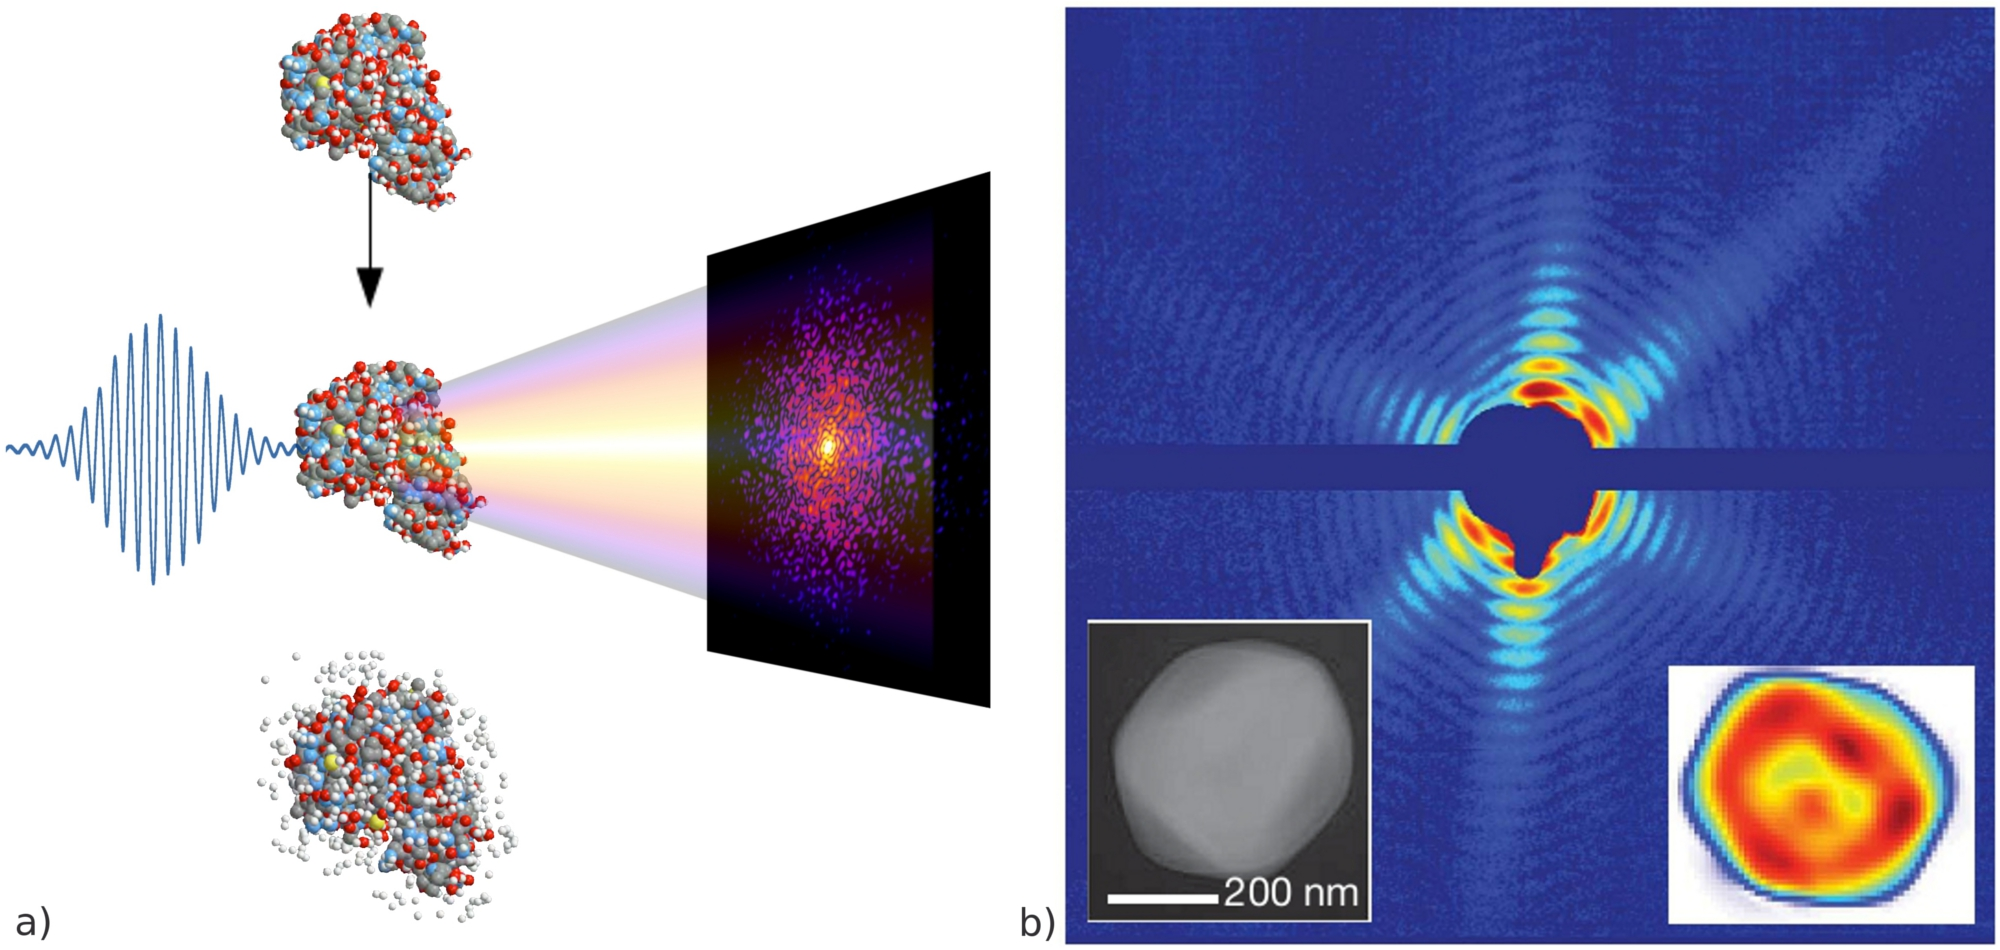
\includegraphics[width=0.80\textwidth]{images/intro-dani.jpg}
	\caption[Conceptual setup of a single particle imaging experiment.]{a) Conceptual setup of a single particle imaging experiment. A nanoparticle is injected and intercepted by an XFEL pulse. The nanoparticle diffracts light before it is destroyed and the diffraction is recorded with a detector. b) Single-shot diffraction image and reconstruction (right inset) of a single Mimivirus. An electron-microscopy image is shown as comparison (left inset). From \cite{Rupp-2013-Thesis,Neutze-2000-Nature,Seibert-2011-Nature}.}
	\label{fig:spi-concept}
\end{figure}
%
But, the highly-intense pulses that enable diffractive imaging lead to new questions. When an intense X-ray pulse irradiates a nanoparticle, the particle will simultaneously absorb and scatter X-rays with the absorption cross-section typically being much larger than the scattering cross-section. From the first moment of light-matter interaction, the absorption will lead to inner atomic-shell vacancies \citep{Young-2010-Nature} and these vacancies make the above mentioned cross-sections time-dependent. Subsequent core-hole decays, such as the Auger decay, typically occur only a few femtoseconds later and the nanoparticle is thus transformed into a nanoplasma on a femtosecond timescale \cite{Bostedt-2012-PRL}. Several forces will ultimately expand the plasma \citep{Gorkhover-2016-NatPho,Ferguson-2016-SciAdv} until eventually, the nanoplasma disintegrates into its atomic components.\\[1\baselineskip]
%
The underlying principle of diffractive imaging, which is that intense X-ray pulses diffract from a single structure before they destroy it\footnote{This is often referred to as ``diffraction before destruction''.} \cite{Neutze-2000-Nature}, demands very short and intense lightpulses \cite{Huldt-2003-JSB,Hau-Riege-2005-PRE}. These will not become available at the currently planned light sources. Therefore, time-dependent scattering factors and trapped or delocalized electrons will affect the diffraction image \cite{Aquila-2015-StrucDyn}. While diffractive imaging is already feasible, these fundamental processes will limit the achievable resolution in single particle imaging. Several ideas have been proposed to address radiation damage in single particle imaging: Atomistic computer models could theoretically account for known damage processes in small systems \citep{Ho-2016-PRA,Quiney-2010-NatPhys,Yoon-2016-scirep}; and sacrificial tamper layers slow the nanoplasma expansion \cite{Hau-Riege-2004-PRE,Hau-Riege-2007-PRL,Jurek-2008-EPJ,Jurek-2009-EPL,Hau-Riege-2010-PRL,Hoener-2008-JPB}. The tamper consists of thin layers surrounding a single particle. When a tampered particle is exposed to intense X-rays, charge-transfer occurs from the photoionized sample to the tamper. The increasingly ionized layers are shed off or sacrificed and radiation damage of the encapsulated sample is retarded (see Figure \ref{fig:tamper-layer}). A part of this thesis is concerned with the investigation of sacrificial layers.\\[1\baselineskip]
%
\begin{figure}
	\centering
		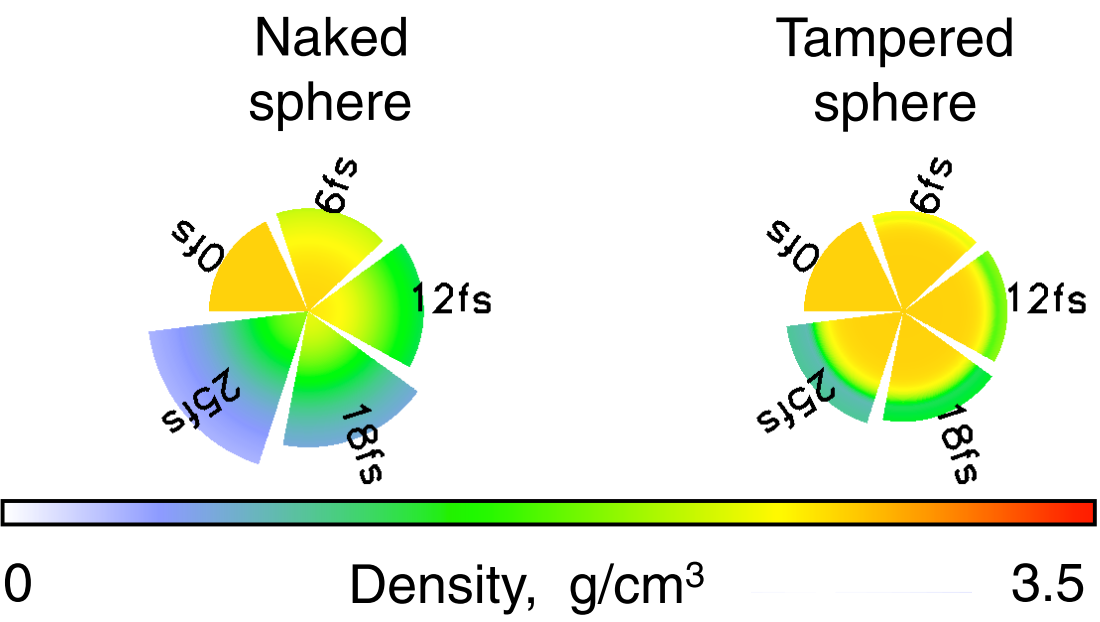
\includegraphics[width=0.80\textwidth]{images/tamper-layer.png}
	\caption[Computer simulations of aluminum spheres with tamper layers]{Computer simulations of \SI{7.5}{\nano\meter} radius aluminum spheres that are illuminated by intense soft X-rays with a fluence of \SI{2.5e8}{\joule\per\square\centi\meter}. On the left is a pristine Al-sphere and on the right is a Al-sphere with a \SI{2.5}{\nano\meter} thick silicon layer (tamper). From \citep{Hau-Riege-2010-PRL}. Reprinted with permission from the American Physical Society (APS).}
	\label{fig:tamper-layer}
\end{figure}
%
An effective sacrificial layer would ideally be thin and uniform around the sample to minimize its background signal. The initial idea of a tamper material was water, since bio-molecules are typically embedded in water-based layers when injected into typical diffractive imaging setups using an aerosol sample jet. However, water-based tampers become disordered in thicker layers and are usually uneven around macro-molecules \cite{Aquila-2015-StrucDyn}. As an alternative, helium layers have been proposed as a tamper material \cite{Mikaberidze-2008-PRA}, but it is unclear if materials with low atomic numbers are a good tamper material \cite{Hau-Riege-2007-PRL}. Currently, aerosol sample jets use helium to dry the injected sample before injection and a next step that is discussed \cite{Bielecki-2016-PC} is to equip a sample with a helium tamper during the injection process.\\[1\baselineskip]
%An alternative is to use helium-based layers, whereby, for example, a sample particle is placed inside a helium-droplet.
%
This thesis discusses the nanoplasma transformation and expansion in solid Xe-, superfluid He- and heterogeneous HeXe-clusters. These rare-gas clusters are a testbed to study nanoparticles in intense X-rays \cite{Fennel-2010-RMP}. Particularly the sacrificial layer physics can be studied with HeXe-clusters. A novel X-ray pump--X-ray probe method \cite{Lutman-2013-PRL} was employed to study the nanoplasma formation in those samples. Here, a pump-pulse triggers a nanoplasma formation and a probe-pulse creates a diffraction image of the system at a later time. Diffraction images and time-of-flight mass spectra are measured coincidentally and are further analyzed. Real-space reconstructions of the clusters are shown with thus far unprecedented resolution and the analysis allows to answer the following questions:
\begin{itemize}
	%\item How does X-ray induced damage compare to optical light induced damage?
	%\item On what timescales do absorption cross-sections change due to X-ray irradiation?
	\item How does an X-ray induced nanoplasma expansion affect the shape of Xe-clusters?
	%\item On what timescales are diffraction images affected at current resolution?
	\item What is the structure of HeXe-clusters?
	\item Does helium act as sacrificial layer in mixed HeXe-clusters?
\end{itemize}
%
This thesis is organized as follows: Chapter \ref{ch:fundamental_concepts} discusses fundamental aspects that are used throughout this study; Chapter \ref{ch:exp_setup} describes the experimental setup at the AMO instrument at LCLS and in particular the so-called ``LAMP'' end-station with its detectors; Chapter \ref{ch:methods} discusses several computational methods; Chapter \ref{ch:results} presents the results of the X-ray pump--X-ray probe study; and Chapter \ref{ch:summary_outlook} summarizes the present work and provides an outlook for further studies.
%
%
%
%\clearpage
\chapter{Fundamental Concepts}\label{ch:fundamental_concepts}
%%%%%%%%%%%%
%- Short introduction what we will go over.
%%%%%%%%%%%%
This chapter condenses the theoretical concepts that will reoccur throughout the present thesis. We start off in section \ref{sec:xfel} with an introduction to the key aspects of X-ray free electron lasers (XFEL), including the beam operating modes self-amplified spontaneous emission (SASE), self-seeding and X-ray pump -- X-ray probe. Section \ref{sec:cluster-theory} is about the formation of rare gas clusters via supersonic jets and pickup sources. We then dive into the interaction of light and matter in section \ref{sec:light-matter-interaction} that discusses coherent, elastic X-ray scattering, and inelastic processes in atoms. The chapter ends with section \ref{sec:ionizatin-of-ext-obj}, describing the nanoplasma formation in pristine cluster and core-shell systems.
%
%
%
\section{Why X-ray free electron lasers?}\label{sec:xfel}
%%%%%%%%%%%%
%- A historic introduction to FELs\\
%%%%%%%%%%%%
%The advance of X-ray free electron laser in the recent years has enabled experimental ideas from long ago but has also opened entirely new branches to research \cite{Pellegrini-2016-RMP,Bostedt-2016-RMP}. So, let us start by investigating how that is. Thus far mostly synchrotron radiation facilities have provided X-rays to a great variety of scientific communities.
%Electromagnetic radiation or light in the X-ray wavelength regime\footnote{Wavelengths of 0.01 of 10nm.} are world famous for their applications in medicine, where X-ray images\index{X-ray!images} allow a non-invasive look inside the body. X-rays are also heavily used in science, where they are heavily used to reveal structures of very small particles, for example proteins - the workhorse bio-molecule in the human body.
X-rays were first created through \textit{Bremsstrahlung}\index{X-ray!Bremsstrahlung}, where an electron beam with kinetic energies $E_{\text{kin}}$ of 100eV - 100keV hit a block of copper and the deceleration of electrons in the copper led to the creation of X-rays. Since then, there has been tremendous progress in the creation of X-rays and they are commonly created in synchrotron facilities for scientific purposes. In a synchrotron facility, electrons are accelerated near the speed of light, $E_{\text{kin}}\text{ > MeV}$ and then injected into a storage ring. The electrons are deflected at bending magnets to circle around the ring. The acceleration at the bending magnet leads to the emission of X-rays. Typically, electrons are bunched together to increase the amount of emitted photons and a storage ring can store many electron bunches allowing a high repetition rate of light pulses on the order of megahertz. The X-ray pulses are characterized through a parameter that is called spectral brightness \cite{Mills-2005-IUCR} or sometimes brilliance\index{brilliance|see{spectral brightness}}. We can define the spectral brightness\index{spectral brightness} as \cite{Als-Nielson-2011-JWS}
\begin{equation}
B = \frac{n}{A\ \Theta\ \Delta\! E},
\label{eq:spectral-brightness}
\end{equation}
with $n$ being the number of photons per second, $A$ the source area, $\Theta$ the divergence of the beam, and $\Delta\! E$ being the spectral bandwidth of the light pulse. The spectral brightness is an overall measure of the quality of a light source. The development of modern synchrotron light sources is hence often measured and compared to previous achieved brightness values. The motivation to improve the spectral brightness is manifold and follows the recipe to let a sample interact with as many photons possible, in the shortest time as possible and with an energy resolution as best as possible. In other words, more brilliant light sources enable imaging of even smaller particles, or investigate dynamics that are even faster.
\begin{figure}[t]
	\centering
		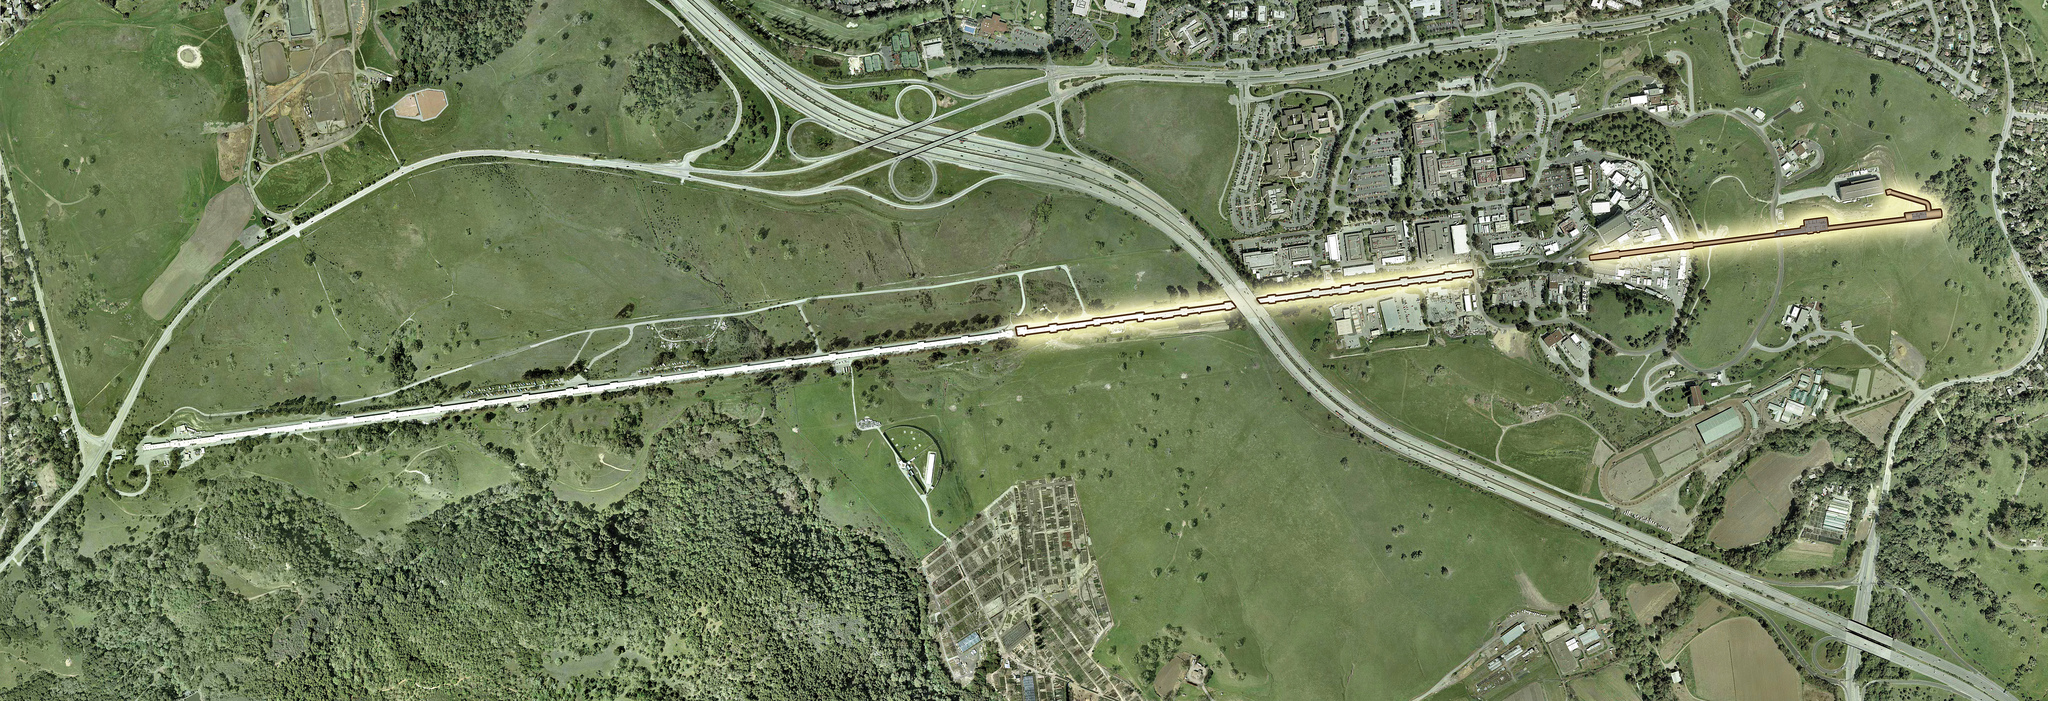
\includegraphics[width=1.00\textwidth]{images/aerial-view-lcls.jpg}
	\caption[Aerial view of the Linac Coherent Light Source.]{Aerial view of the Linac Coherent Light Source\index{Linac Coherent Light Source} (LCLS). LCLS\index{LCLS|seealso {Linac Coherent Light Source}} uses the last third of the SLAC Linear Accelerator but is overall a $\sim 4.1$ km long machine. The accelerator and buildings are stretched far because of the light generation process. From \cite{SLAC-2009-Flickr}}
	\label{fig:aerial-view-lcls}
\end{figure}
To get a numerical understanding, let us look at non-linear absorption dynamics in atoms and molecules. One can conservatively estimate that a typical absorption cross section at soft X-rays\footnote{X-rays with wavelengths of 10nm to 0.2nm.} is around $\sigma = 1$ megabarn (Mb) \cite{Bucksbaum-2011-Book}. Typical X-ray focii are\footnote{Focus size at the AMO endstation at LCLS.} $A = 1\ \mathrm{\mu m}^{2}$ such that the number of photons, $n_{in}$, needed to absorb just one photon per atom, $n_{abs}$, is
\begin{equation}
n_{in} = \frac{n_{abs} A}{\sigma} = \frac{10^{-8} \mathrm{cm}^{2}}{10^{-18} \mathrm{cm}^{2}}=10^{10}\qquad \mathrm{photons.}
\label{eq:absorption-cross-section}
\end{equation}
We can compare this to a modern synchrotron source, e.g., NSLS-II. This synchrotron produces $1.7 10^{4}$ photons per pulse in the Si(111) bandwidth at pulse durations of a few tens of picoseconds \cite{Williams-2016-PC}. That is far out of reach for investigating non-linear, or multi-photon, processes. While this back of the envelope type of calculation might be off by an order of magnitude or so depending on the specific case, it illustrates the order of magnitude improvement scientists were looking for to unravel entirely new aspects of nature. As it is not possible to use conventional optical methods to increase the number of X-ray photons there were drastic ideas. A progressive United States defense program in the 80's ignited an atomic bomb to create an X-ray beam that was intended for use as anti-(space)missile defense \cite{Hecht-2008-OPN}. In a similar time, it was also proposed to build free electron laser \cite{Kondratenko-1980-PA,Bonifacio-1984-OC} to increase the spectral brightness.

Free electron lasers, amplify the light along a straight line to create optical laser-like radiation. Construction of the first hard XFEL finished in 2009 and it is called the Linac Coherent Light Source\index{Linac Coherent Light Source}. LCLS can be seen from a birds-eye view in figure \ref{fig:aerial-view-lcls}. XFEL are able to create $10^{12}$ photons per pulse and achieve pulse lengths of a few femtoseconds. The beam parameters of the XFEL increased the spectral brightness of user facilities by many orders of magnitude\footnote{See figure \ref{fig:soft-xray-self-seeding} for an illustration of the improvement in brilliance.}. This allows the study of, for example, the ultrafast movement of electrons in chemical reactions \citep{Dell'Angela-2013-Science,Picon-2016-NatComm}, the imaging of nanoparticles \citep{Chapman-2011-Nature,Seibert-2011-Nature} and the discussed nonlinear dynamics of atoms, molecules and clusters \citep{Young-2010-Nature,Rohringer-2012-Nature,Berrah-2011-PNAS,Gorkhover-2012-PRL}.\\[1\baselineskip]
Few XFEL exist today. LCLS at SLAC National Accelerator Laboratory in the United States and SACLA at RIKEN in Japan are the two currentlz operating user facilities. Due to their success, more XFEL are being build around the world. The European XFEL near DESY\footnote{abbreviation for Deutsches Elektron Synchrotron} in Germany, the SwissFEL at Paul Scherrer Institut in Switzerland and the PAL-XFEL at Pohang Accelerator Laboratory in South Korea are noticable XFEL that are being build at user facilities.
%
%
%
\subsection{From bending magnets to undulators}\label{sec:undulator}
%%%%%%%%%
%- Idea and schematic setup\\
%- Explain SASE including micro-bunching\\
%- Talk about the importance of monitoring the energy loss
%%%%%%%%%
\begin{figure}[t]
	\centering
		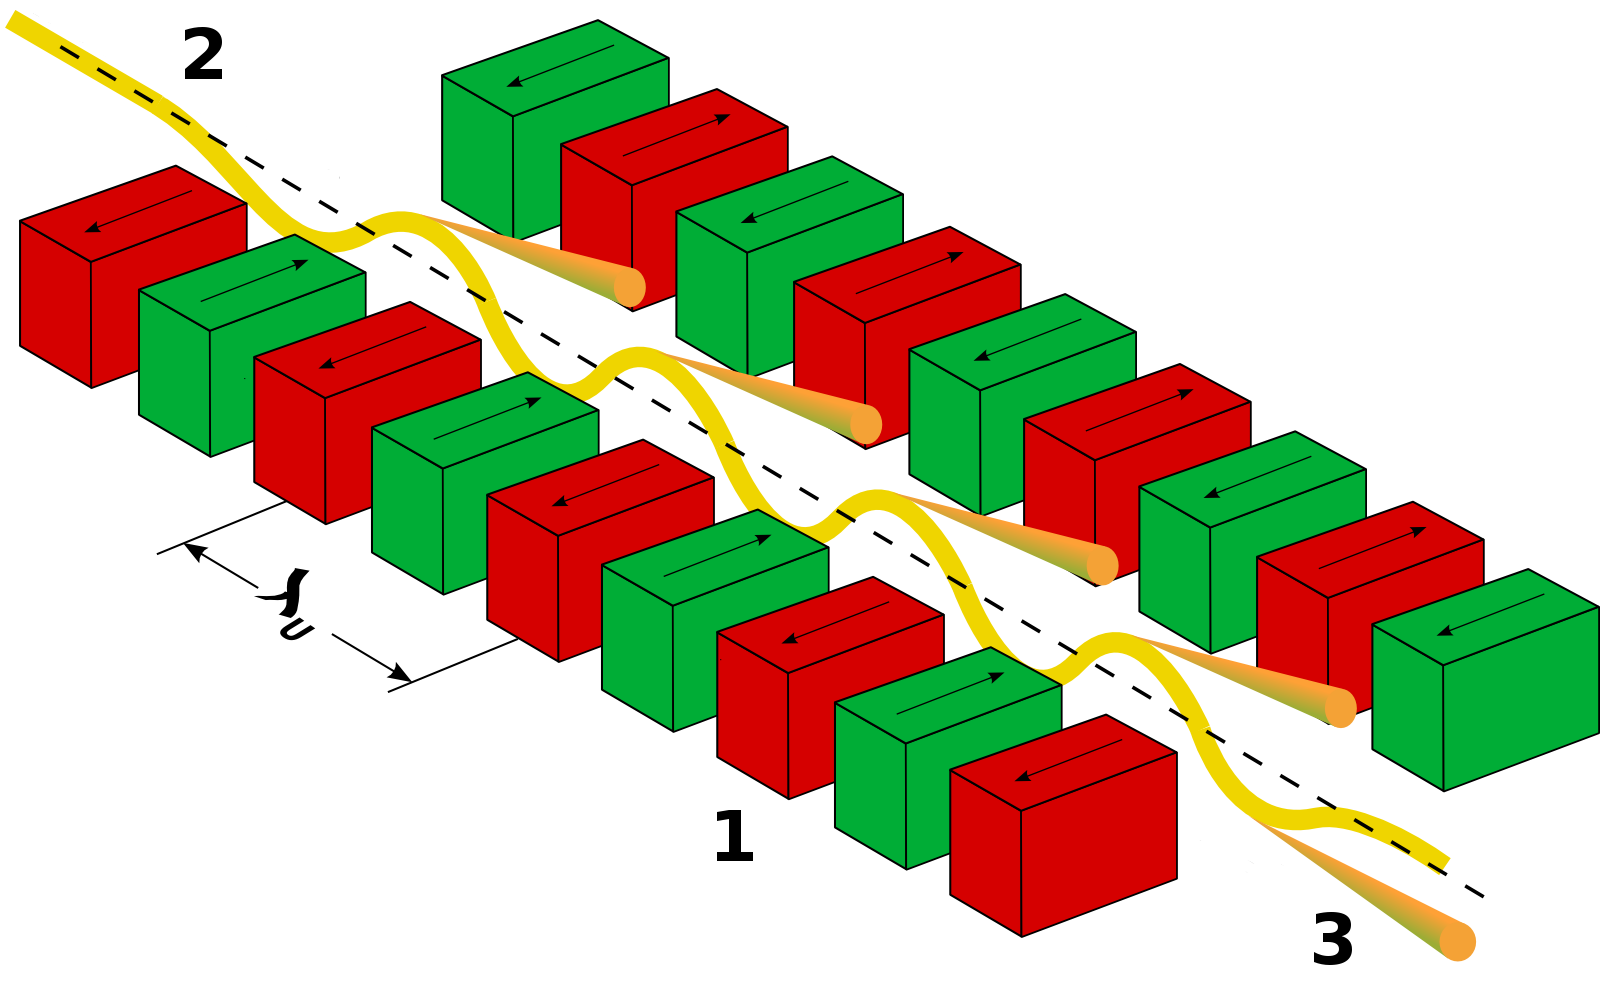
\includegraphics[width=1.00\textwidth]{images/Undulator.png}
	\caption[Schematic setup of an undulator.]{Schematic setup of an undulator with a period of $\lambda_{U}$. (1) Magnets in alternating polarity; the arrows indicate the direction of the magnetic field. (2) Incoming electron bunch near the speed of light. (3) Emitted light in beam direction due to sinusodial movement of the electron bunch. From \cite{holst-2005-wiki}.}
	\label{fig:undulator}
\end{figure}
In the beginning of X-ray lightsources\index{lightsource} the radiation was generated using bending magnets\index{bending magnets}. Therefore a bunch of electrons was accelerated near the speed of light and traversed a bending magnet. The acceleration from the magnet resulted in the emission of electro-magnetic radiation. The first improvement to creating X-rays at a bending magnet was through a \textit{wiggler}\index{wiggler}. Wigglers consist of magnets that are arranged in an alternating order. An electron bunch that is traveling through a wiggler is wiggled along its path due to magnetic fields, which causes the particles to emit radiation. Wigglers can be considered as a series of bending magnets, which is why the total emitted power $P_{emitted}$ is proportional to the number of magnets $m$ \citep{Brown-1983-NIMPR}
\begin{equation}
P_{emitted} \propto m,\quad \mathrm{in\ a\ wiggler\ magnet}.
\end{equation}
The emitted radiation has a broad, continuous spectrum and the center of that spectrum can be controlled by changing the speed or kinetic energy of the electron bunch. Wigglers have been used at the Stanford Synchrotron Radiation Lightsource (SSRL) in 1979 to generate X-rays. Independently from wigglers, undulators\index{undulator} were developed \citep{Williams-2009-xb}. A schematic setup of an undulator can be seen in figure \ref{fig:undulator}. Wigglers and undulators create radiation because of the same principle, an electron bunch is accelerated near the speed of light and then forced on a sinusoidal pathway. In undulators, the separation of magnets is specific and named undulator period $\lambda_{U}$. The undulator period and magnetic fields are chosen such that the emitted radiation per period constructively interferes with each other. Thus the emitted power $P_{W}$ now scales with \citep{Kim-1986-NIMPRA}
\begin{equation}
P_{\text{emitted}}\propto m^{2},\quad \mathrm{in\ an\ undulator\ magnet}
\end{equation}
The emitted wavelengths of undulators have a more narrow spectrum and a higher flux than wigglers. We can further characterize undulator (and wiggler) by the strength parameter $K$, which is given by \citep{Huang-2007-PRSTAB}
\begin{align}
K &= \frac{e\ B_{\text{max}}\ \lambda_{U}}{2 \pi\ m_{e}\ c},
\intertext{with $e$ being the elementary charge, $B_{\text{max}}$ being the maximum magnetic field in the undulator (wiggler), $m_{e}$ being the mass of an electron and $c$ being the speed of light, we can write in convenient units}
K &\approx 0.934 B_{max}\ \lambda_{U}\qquad \left[\mathrm{T\ cm}\right].
\label{eqn:undulator-strength}
\end{align}
Undulators typically have $K<1$ Tcm (and wiggler $K\gg1$ Tcm). Undulator magnets are large constructs of a few meters and their undulator period is on the order of centimeter. The electrons emit radiation in the nanometer wavelength regime because the electrons near the speed of light have to be considered relativistic. In view of the electrons the undulator period $\lambda_{U}$ appears shorter. We can account for the relativistic effects and express the resonantly amplified wavelength $\lambda_{r}$ by \citep{Huang-2007-PRSTAB}
\begin{equation}
\lambda_{r} = \frac{\lambda_{U}}{2 \gamma}\left(1+\frac{K^{2}}{2}+\gamma^{2}\Psi^{2}\right),\label{eqn:fundamental-wavelength}
\end{equation}
with the kinetic energy $\gamma$ of the electron bunch in the undulator and the electrons observation angle $\Psi$.\\
%Summarizing, modern lightsources use undulators to generate radiation as these magnets create more photons that have a narrow spectral bandwidth compared to bending magnets and wiggler. Undulators are characterized by the strength parameter given in equation \ref{eqn:undulator-strength}, which is only dependent on the undulator gap $\lambda_{U}$ and the magnetic field $B$. The fundamental amplified wavelength is given by the resonance condition equation \ref{eqn:fundamental-wavelength}.\\
\begin{figure}
	\centering
		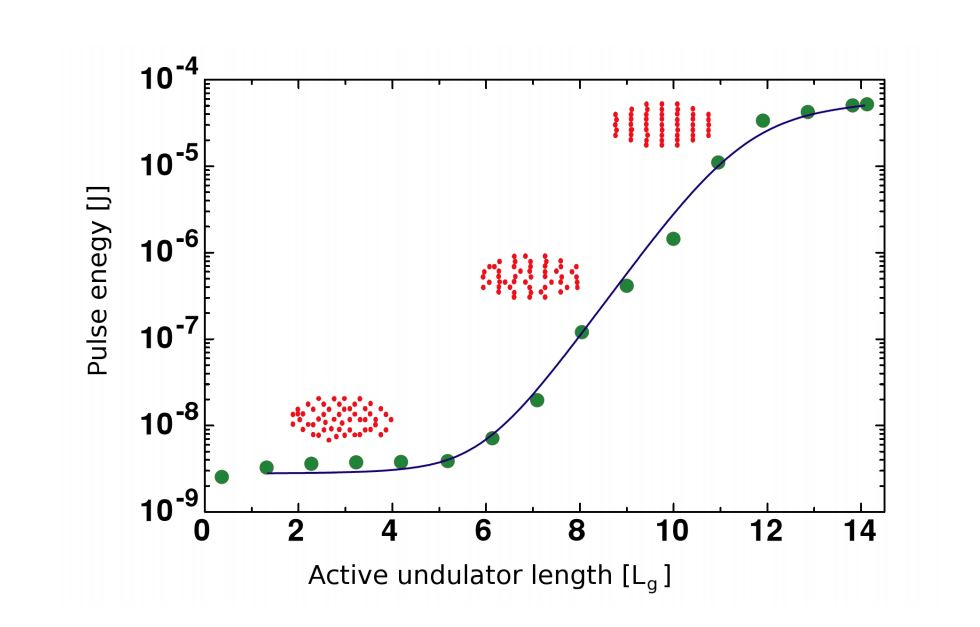
\includegraphics[width=0.75\textwidth]{images/gain-length.JPG}
	\caption[Undulator gain curve correlated to microbunching.]{Undulator gain curve correlated to microbunching. The X-ray pulse energy is plotted logarithmically over the undulator length $L_{g}$ (blue curve, green dots) and shows an exponential growth until saturation. The electron bunch (red dots) starts with a random density distribution. As the bunch travels through the undulator, its density is modulated periodically such that the electrons microbunch. Upon optimal \textit{microbunching}, the X-ray lasing process saturates. From \citep{Rupp-2013-Thesis,Rupp-2016-Springer}}
	\label{fig:gain-length}
\end{figure}
\subsection{Self amplification by spontaneous emission}\label{sec:sase}
If an electron bunch travels through just one undulator, the emitted power scales linearly with the number of electrons $N_{e}$, which is due to the finite size and randomly distributed density of an electron bunch. If the electrons emit light from the same point or separated by $n\ \lambda_{r}$ $\left(n=\left\{1,2,3,...\right\}\right)$ the emitted photons would constructively interfere. FEL use this idea to generate their light pulses. FEL have a straight and long undulator section\footnote{LCLS has a 112m long undulator section.}, where multiple undulators are connected in series. As the electron bunch travels through the FEL undulator section, microscopic effects play a role that could be neglected in typical synchrotron radiation sources. In vacuum, light will always be faster than electrons near the speed of light. This slight velocity difference means that the co-propagating photons and electrons have a phase difference and interact with each other. Depending on the phase, an electron will either gain or loose velocity. Over each undulator period, we can describe this \textit{slippage}\index{slippage} with $\lambda_{r}(\Psi = 0)$. As a result, the initial uniform electron density is periodically modulated as it travels through the undulators of a FEL. The modulated electron bunch structure is called \textit{microbunching}\index{microbunching}. The increasingly structured electron beam amplifies a more narrow wavelength bandwidth and the number of electrons that are in phase with the photons increases over the travel length through the undulator. The lasing process saturates when the microbunching is fully developed. This process is illustrated in figure \ref{fig:gain-length}.
The microbunching is defined by the initially emitted photons of pseudo-random wavelength, since the bunch amplifies these specific wavelengths as it travels through the undulators through subsequent spontaneous emission.
%Initially (random) created photons in the undulator define the microbunching as it travels through the undulators and amplifies these photons through subsequent spontaneous emission. 
Hence, this type of radiation (or FEL operation mode) is called \textit{Self Amplification by Spontaneous Emission} (SASE). SASE achieves laser alike amplification of the radiation power $P_{SASE}$ scales \citep[see][p.~61]{Als-Nielson-2011-JWS}
\begin{equation}
P_{SASE} \propto N_{e}^{2},\quad \mathrm{SASE\ operation}
\end{equation}
SASE spectra can be seen in figure \ref{fig:SASE-spectra}. A SASE spectrum is different from shot-to-shot and has distinct peaks that are defined by the initial photons on top of a more broad background.
\begin{figure}
	\centering
		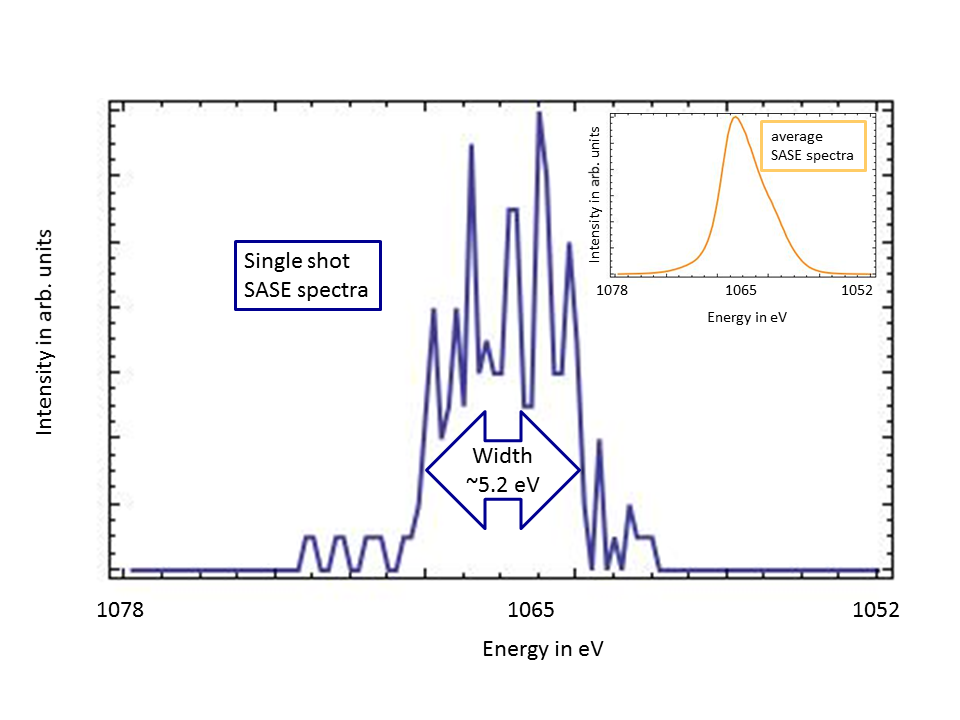
\includegraphics[width=0.80\textwidth]{images/SASE-spectra.png}
	\caption[SASE single-shot and average spectra]{The large blue spectra is a SASE spectra from a single LCLS shot measured with a photoelectron \citep[see][]{Bucher-2014-Unpublished}. Note the spiky peak structure on a background pedestal. Within the narrow bandwidth of a FEL pulse some energies are more strongly amplified due to the microbunching. The yellow graph in the inset is an average spectrum of several hundred single-shots and shows a low energy tail, which is due to FEL-jitter.}
	\label{fig:SASE-spectra}
\end{figure}
The electrons interact with the light field because of their narrow spatial and kinetic energy distributions that define the so called \textit{emittance}\index{emittance} of an electron bunch. Only the linear accelerator of FEL are able to compress an electron bunch in space and energy, i.e. create a low emittance electron bunch, such that it can interact with the photons and microbunch. Since the creation of X-rays affects the kinetic energy of the electron bunch $\gamma$ and the lack of optics, XFEL use one (compressed) electron bunch\footnote{the European XFEL uses a so called bunch train, where multiple electron bunches are accelerated in series.} in a long set of undulators to create one light pulse. This is also called a \textit{single-pass high-gain} FEL. Without going into much detail, optics can be used to build \textit{multi-pass low-gain} FEL that are able to reuse electron bunches \citep{Kim-2008-PRL}, which leads to higher repetition rates and more narrow spectrum but fewer photons per pulse.
%
%
%
%
\subsection{Soft X-ray self seeding}
%%%%%%%%%%%%%%%%%%%%%%
%- Should I include this section? I could use it for the pump probe as well\\
%- Self seeding vs. seeded FELs\\
%- Schematic setup of a self seeding unit\\
%- Work towards self-seeded beams including spectrometer data
%%%%%%%%%%%%%%%%%%%%%%
\begin{figure}
	\centering
		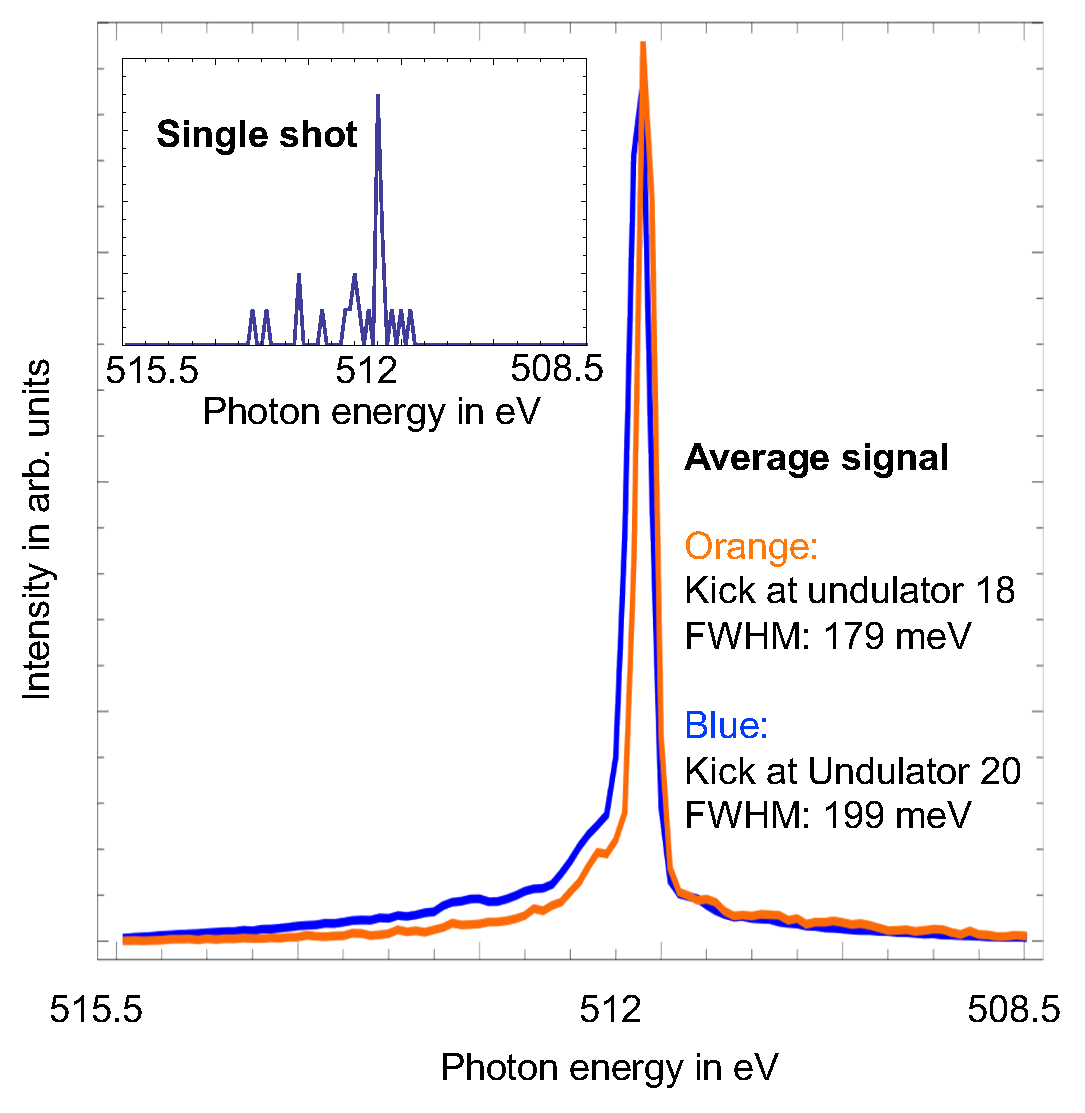
\includegraphics[width=0.49\textwidth]{images/Soft-X-ray-self-seeding.pdf}
		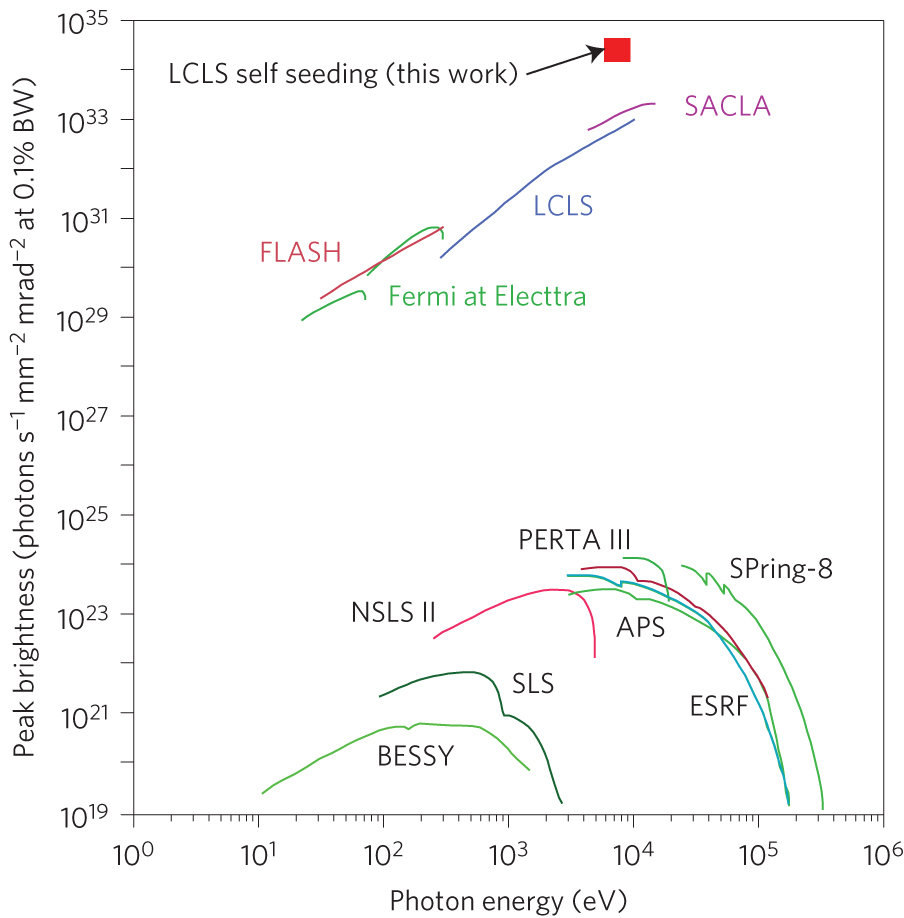
\includegraphics[width=0.49\textwidth]{images/spectral-brightness-fletcher-2015.jpg}
	\caption[Soft X-ray self-seeding spectra and brilliance of various lightsources.]{Left, normalized average spectra of soft X-ray self-seeding (SXRSS) operations using the AMO instrument at LCLS \cite[see][]{Bucher-2014-Unpublished}. The self-seeding spectra is characterized by a sharp spectral peak around a desired energy accompanied by a SASE radiation type spectral pedestal. The often undesired SASE pedestal is suppressed, when the electron bunch travel through undulators is shortened. The right image shows the peak spectral brightness of various light sources over a wide photon energy range. SXRSS operations has a spectral brightness that exceeds current SASE FEL sources. From \citep{Fletcher-2015-NatPho}.}
	\label{fig:soft-xray-self-seeding}
\end{figure}
Another FEL beam mode is the seeded type. In contrast to the SASE operation, where the initial photons are randomly emitted and further amplified, a seeded FEL starts with a given \textit{seed} of photons. If the set of initial photons is monochromatic, mostly this wavelength is amplified as the bunch travels through the undulator along the seed. The initial photon seed can be created through various processes and the wavelength of the photon seed is the critical parameter in determining which method to choose. For example, in the infra red (IR) to extreme ultra violet (XUV) regime, conventional lasers can be used to place the initial photons seed. However, due to the lack of lasers available at X-rays wavelength regimes, the idea of \textit{self-seeding}\index{self-seeding} gained traction. In self-seeding, an electron bunch is first send through a few undulator magnets to generate a few SASE photons, the electrons and photons are then separated using a magnetic chicane, which also neutralizes the microbunching in the electron bunch. The monochromator selects a small wavelength slice from the comparably broad SASE spectrum of the initial photons. Photons exiting the monochromator are considered as \textit{seed}. The seed and the electron bunch are overlapped again using the magnetic chicane and then send through more undulators. Here, the seed modulates the electron bunch and thus only a narrow spectral band is amplified. A typical spectrum of a soft X-ray self-seeded beam can be seen in the left figure \ref{fig:soft-xray-self-seeding}. The characteristics of a self-seeded spectrum are an intense peak at the selected wavelength regime on top of a broad SASE background pedestal. The background is an artifact of the amplification of some spontaneous emission events and can be suppressed by using fewer undulator magnets. Self-seeded beams have a significantly reduced pulse energy by an order of magnitude, depending on the exact beam parameters, as compared to LCLS SASE operations. However, in their main peak, self-seeded beams have a higher spectral brightness when compared to a SASE spectrum. Using equation \ref{eq:spectral-brightness} the increase in spectral brightness compared to SASE is understandable and it is illustrated in the right figure \ref{fig:soft-xray-self-seeding}. Self-seeded beam operations have recently been demonstrated at LCLS. At hard X-rays, the Hard X-Ray Self-Seeding (HXRSS) instrument uses a diamond crystal to select a wavelength slice \citep{Amann-2012-NatPho}. At soft X-rays, the Soft X-ray Self Seeding (SXRSS)\index{self-seeding!soft x-ray} instrument uses a grating as dispersive element \citep{Ratner-2015-PRL}. A seeded beam using an external laser generate photons as initial seed has been demonstrated at the extreme ultra violet (XUV) FEL FERMI at Ellettra-Sincrotrone in Italy \citep{Allaria-2012-NatPho}. The peak intensity in a narrow spectral band makes seeded beams interesting for a variety of applications particular in condensed matter physics, where it is instrumental to excite with narrow bandwidth photons. Of course there are also applications in atomic and molecular physics, ranging from linear absorption spectroscopy \citep{Ferguson-2014-Unpublished}, to ultrafast photoemission spectroscopy on molecules \citep{Bucher-2014-Unpublished}, to non-linear stimulated Raman spectroscopy \citep{Kimberg-2016-FD}, to ultra-fast photoemission studies. Particular interesting for this work is the magnetic chicane from the SXRSS instrument that has been used as described in the next chapter.
%
%
%
%
\subsection{Novel X-ray pump–probe techniques}\label{sec:novel-pump--probe-tech}
%%%%%%%%%%%%%%%%%
%- Albertos pump-probe version\\
%- Agos two color pump probe version\\
%- Ratners and Agos seeded pump probe version\\
%- Use spectra from single-shot spectrometer
%%%%%%%%%%%%%%%%%%%%%%%%
In order to study X-ray induced phenomenon using X-ray imaging and spectroscopy techniques, as it is discussed in the present work, two X-ray pulses are needed . Here, a pump pulse is used to induce dynamics in the sample system and a probe pulse is used to probe them at a certain time delay $\Delta t$. Pump--probe experiments are commonly used as they allow a precise study of dynamics. The pump pulse gives a very controllable starting point, i.e. time zero in the dynamic process, and the probe pulse can perform a measurement at a later time delay $\Delta t$. Sometimes pump and probe pulse are switched, which is indicated by a negative time delay $\Delta t$, often to verify time zero or to probe the system before any dynamics have occurred.\\
Creating two X-ray flashes to create a pump--probe experiment is a technical challenge and again this challenge is due to the lack of X-ray optics. In order to overcome this challenge, two methods have been proposed. Method one, mirror based beam-split and delay systems \citep{Castagna-2013-JPCS,Murphy-2012-SPIE} that split one pulse into a pump and probe beam and allow the delay of the latter. These systems are typically limited to short times delays, as the optics have to fit into existing setups and have a low transmission of X-rays over the mirrors. Method two, uses accelerator based schemes \citep{Lutman-2013-PRL,Marinelli-2015-NatComm} that manipulate electron bunches to create two X-ray pulses. Limitations arise depending on the scheme, e.g. limited pulse delay $\Delta t$ or pulse energy split through limited electron beam separation or length of magnetic chicane. Both methods have been demonstrated at LCLS and have found use to complement the more widely available optical laser pump -- X-ray probe methods particularly in the chemical sciences \cite{Picon-2016-NatComm,Ferguson-2016-SciAdv,Liekhus-Schmaltz-2015-NatComm}.\\
Another aspect to pump--probe experiments is the tunability of wavelengths in each pulses, for example to resonantly pump and off-resonance probe or vice versa. Equation \eqref{eqn:fundamental-wavelength} indicates which parameters can be tuned to create two pulses of different color. One, the undulator parameter K can be tuned to change the emitted wavelength, or two, the lorentz factor $\gamma$ can be different if there are two electron bunches. A potential third option are variable gap undulators that allow a change of period $\lambda_{U}$. At LCLS $\lambda_{U}$ is fixed but future upgrade plans for LCLS-II include variable gap undulators \citep{Galayda-2014-IPAC}. As the accelerator based X-ray pump -- X-ray probe method, let us describe these schemes in greater detail.
%
%
%
\subsubsection{Undulator parameters $K_{1,2}$ based pump--probe scheme}
\begin{figure}
	\centering
		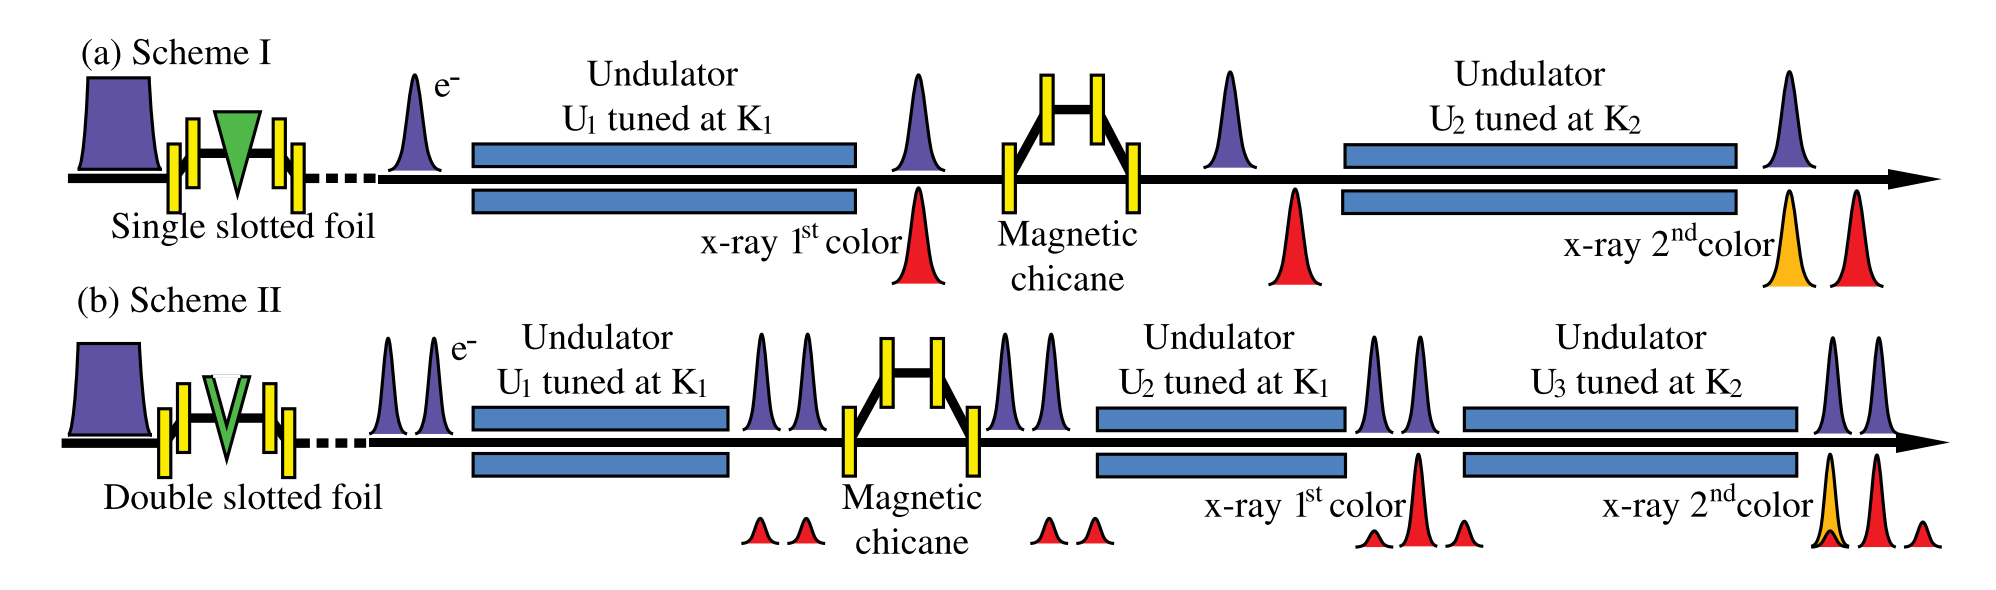
\includegraphics[width=1.00\textwidth]{images/Albertos-pump-probe-scheme.png}
	\caption[Schematic setup of an undulator based pump--probe scheme.]{Schematic setup of undulator parameter $K_{i}$ based pump--probe schemes at LCLS. Scheme I) creates one electron bunch using a single slotted foil and scheme II) creates two electron bunches using a double slotted foil. The electron bunches emit radiation with a wavelength depending on $K_{i}$. A time delay $\Delta t$ between pulses is introduced using a magnetic chicane. From \cite{Lutman-2013-PRL}. Reprinted with permission from APS.}
	\label{fig:Albertos-pump-probe-scheme}
\end{figure}
The first developed accelerator based pump--probe technique at LCLS \cite{Lutman-2013-PRL} uses a difference in undulator parameters $K_{1,2}$ to create two pulses of different wavelength, the time delay is introduced through a magnetic chicane and a schematic setup can be found in figure \ref{fig:Albertos-pump-probe-scheme}.\\
Following the figure, in scheme I, one electron bunch is created through a single slotted foil\footnote{A single slotted foil or emittance-spoiling foil works comparable to a monochromator. It leaves a certain energy band of the electron bunch within the slot unspoiled and Coulomb scatters or spoils (compare to apertures) the rest. The 'dispersive' element is a magnetic chicane. By narrowing the electron beam one also reduces its pulse duration \cite{Emma-2004-PRL}.}  The use of the slotted foil enables control over the pulse duration. The electron bunch then travels through an undulator section $U_{1}$ tuned at strength parameter $K_{1}$ and is stimulated to lase but the process does not go into saturation such that the electron bunch can be reused in the second undulator section. A magnetic chicane removes the microbunching from section $U_{1}$ such that in undulator section $U_{2}$, tuned to undulator strength parameter $K_{2}$, the electron bunch lases again and the process is able to saturate. The maximal color separation between the two pulses is $~ 1.9\%$ in relative difference between $K_{1}$ and $K_{2}$.\\
The time delay $\Delta t$ between the two pulses is introduced by a magnetic chicane. At LCLS, a dedicated chicane, e.g. from the soft X-ray self-seeding instrument, can reach up to
\begin{equation}
\Delta t_{\text{max}} = 800 fs.
\label{eq:alberto-delta-t-max}
\end{equation}
The minimal time delay can be achieved by setting the deflection in the magnetic chicane to zero in which case
\begin{equation}
\Delta t_{\text{drift}} = \frac{l}{v_{\text{el drift}}} - \frac{l}{c}\approx 0 fs,
\label{eq:alberto-delta-t-min}
\end{equation}
with $l\approx 4m$ being the length between undulator sections $U_{1}$ and $U_{2}$ and $c$ being the speed of light and $v_{\text{el drift}}$ being the drift velocity of the electron bunch. As the electron bunch travels close to the speed of light $t_{\text{min}}$ is typically on the tens of attosecond timescale. The timing jitter between the two light pulses using only one electron bunch comes from the magnetic chicane due to the magnetic field jitter and the electron beam energy jitter. The total contribution to the timing jitter is less than $0.4\%$ of the time delay $\Delta t$ imposed by the chicane. Since the delay chicane does not significantly contribute to the delay $\Delta t_{\text{min}}$ a bigger factor is the velocity mismatch of the light pulse and the electron bunch. This mismatch can be estimated by
\begin{equation}
\Delta t_{\text{min}}-t_{\text{drift}}=\frac{N_{u} \lambda_{r}}{c},
\label{eq:alberto-beam-missmatch}
\end{equation}
with $N_{u}$ being the undulator periods. Given the parameters in study \cite{Lutman-2013-PRL}, $t_{\text{min}}=3fs$ such that a partial overlap between the electron bunch and lightpulse could be achieved after the magnetic chicane. It should be noted that this technique has been used in the described experiment.\\
Scheme II uses a double slotted foil\footnote{A double slotted foil works as a single slotted foil but it leaves to parts of the electron beam unspoiled through the two slots.} to create two electron beams. The two beams have a longitudinal separation that translates into the time delay $\Delta t$. The electron bunches travel through a first set of undulators $U_{1}$ that creates two pulses of the same wavelength, due to the shortness of the section $U_{1}$ the lasing process does not saturate. The electron bunches are then delayed using a magnetic chicane such that the leading electron bunch overlaps with the trailing light pulse. This light pulse now functions as a seed for the leading electron bunch such that this pulse saturates in undulator section $U_{2}$. The electron bunches then travel through the magnets at $U_{3}$, where the trailing electron bunch creates a second saturated pulse, the leading electron bunch barely emits radiation in $U_{3}$ since its energy spread has become too large after lasing in $U_{2}$. Using this method, two saturated lasing pulses can be generated, however, temporal overlap cannot be achieved.
%
%
%
%
\subsubsection{Twin bunch or Lorentz factor $\gamma$ based pump--probe scheme}
\begin{figure}
	\centering
		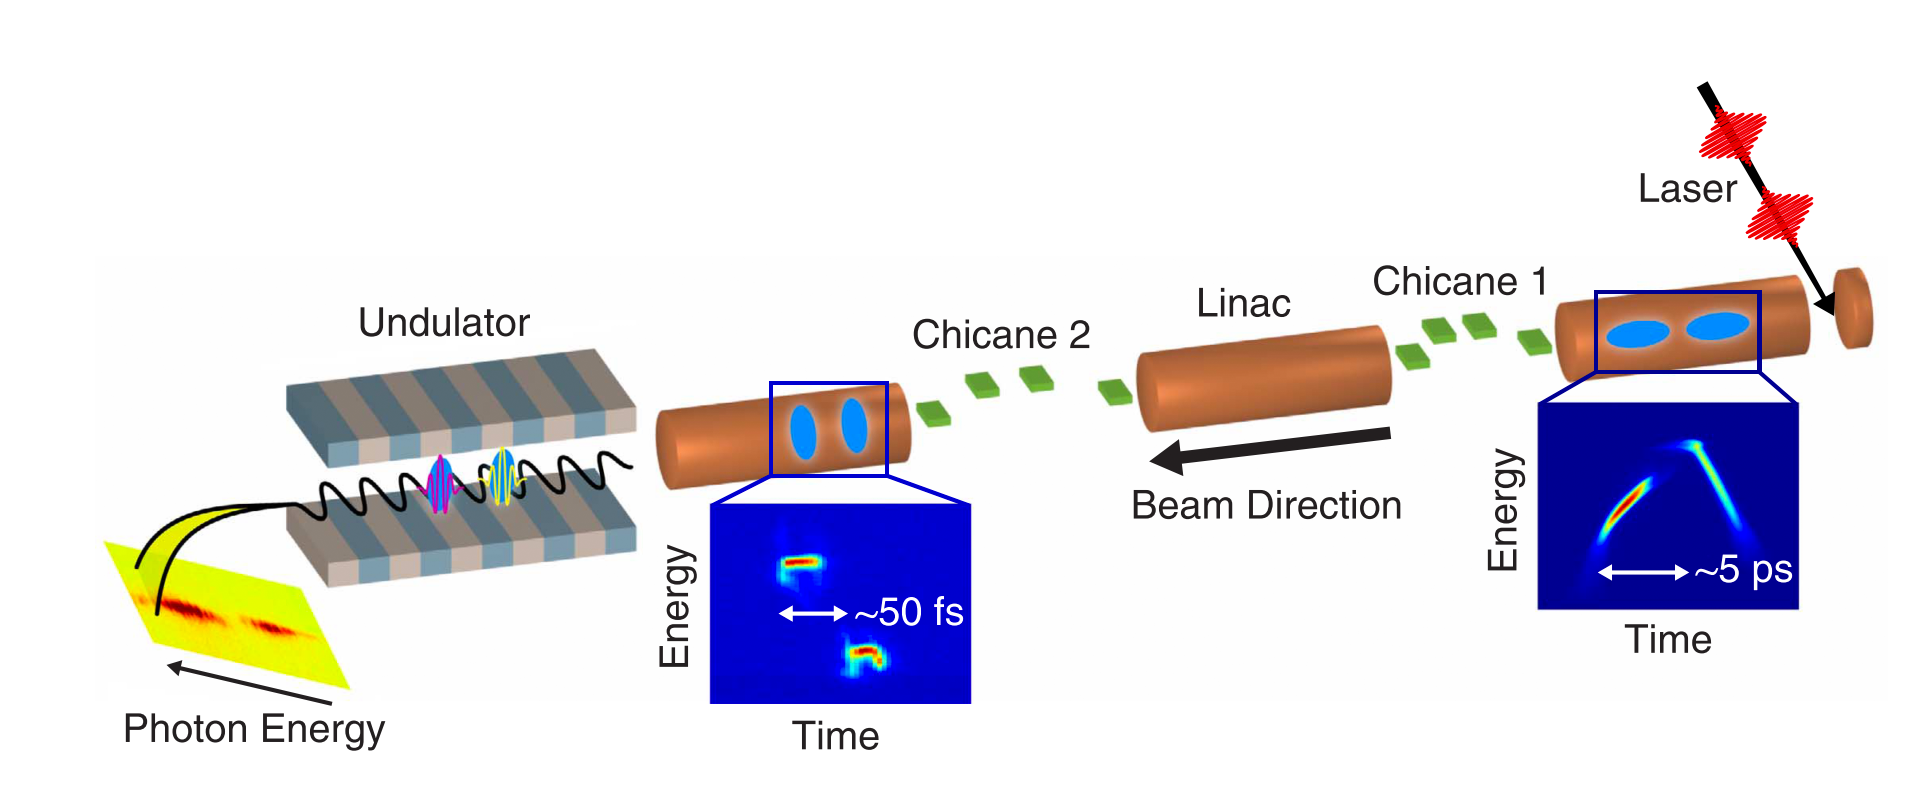
\includegraphics[width=1.00\textwidth]{images/Agos-pump-probe-scheme.png}
	\caption[Schematic setup of a bunch based pump-probe setup.]{Schematic setup of the two bunch, two color pump--probe setup at LCLS. Two laser pulses shot at a cathode create two electron bunches with a delay $\Delta t$ on the picosecond timescale. Two magnetic chicanes compress the bunches such that a delay $\Delta t$ is on the ten femtosecond timescale. Both pulses go through one undulator section and the lasing process is saturated. The relative color separation is on the order of $1\%$ between the bunches. From \citep[\href{http://creativecommons.org/licenses/by/4.0/}{\ccby}]{Marinelli-2015-NatComm}.}
	\label{fig:Agos-pump-probe-scheme}
\end{figure}
The second developed accelerator-based pump-probe technique at LCLS \cite{Marinelli-2015-NatComm} uses two electron bunches of different energy. A schematic setup of this beam operation can be found in figure \ref{fig:Agos-pump-probe-scheme}.\\
The electron bunches are created through a double laser pulse that impinges on a photocathode. Initially, these two bunches have a time delay of a few picoseconds, however, two magnetic chicanes compress the electron bunches in the time and intensity domain such that a time delay on the ten femtosecond timescale is achieved. The electron bunches then travel through one undulator section and both pulses saturate in their lasing process. At $8.3k$ eV, both pulses combined can reach pulse energies of $1.2mJ$, the color separation is $100$ eV and the time separation ranges from $\Delta t_{min}=0fs$ to $\Delta t_{max}=100fs$. At hard X-rays, this method requires the pump pulse to have a higher photon energy than the probe pulse, although their respective intensities may vary. However, this method is not restricted to hard X-rays and can be utilized at soft X-rays. In soft X-rays, the slotted spoiler foil can be used. This enables further control over the electron bunches and allows crossing time zero with both pulses.
%%%
\section{Rare gas clusters}\label{sec:cluster-theory}
%%%%%%%%
%- Why are rare gas clusters a suitable sample
%%%%%%%%
Clusters have a long history as a sample to study light-matter interaction for a few reasons. Their characteristics are well known, they can form interesting states and often it has practical purposes \cite{Haberland-1994-Springer}. Generally speaking, clusters are an aggregation of atoms or molecules and vary in size. Their size ranges from a few atoms to mesoscopic sizes such that one can classify a cluster as a bulk material. Even though clusters can form exotic materials that are interesting to study, they can be simulated with computer models. Besides these testbed characteristics, clusters can be created comparably easily and are tunable in size. Rare gas clusters are a subclass of clusters and they are bound by van der Waals forces, thus are normally neutral-charged. Single van der Waals cluster typically form in an icosahedral\footnote{An icosahedron is a polyhedron with 20 faces, i.e. a dice with 20 faces.} shape when they are sufficiently small (up to nanometer sized) \cite{Miehle-1989-JCP} and have mostly a fcc-crystal\footnote{fcc is short for face-centered cubic. A very common crystal structure.} structure but exhibit also hcp-crystal\footnote{hcp stands for hexagonal close-packed and is also a crystal structure.} structures \cite{VanDeWaal-1993-JCP,Krainyukova-2006-TSF}. In the present work, superfluid helium cluster (or droplets), solid xenon cluster and a mixture of both have been used as a sample. Therefore, we shall explore the creation of homogenous and heterogeneous rare gas clusters in the next sub-sections.
%
%
%
\subsection{Generation of homogenous cluster}\label{sec:homogenous-cluster}
%%%%%%
%- the theory behind rare gas cluster creation.
%%%%%%
Rare gas clusters, for example xenon clusters, can be generated in a variety of ways. Often, as in the described experiment, rare-gas clusters are created by releasing gas from a reservoir into a vacuum. Here, a nozzle connects the gas reservoir with the vacuum system and while the gas is expanding through the nozzle, many collisions take place. So, the cluster formation process can be explained intuitively through a kinetic model \cite{Lippmann-1984-JCP}. In other words, clusters grow through collisions with monomer, dimer and other clusters. We can express a collisions mathematically through the following reaction formula
\begin{align}
A_{n}+A_{m} \rightleftharpoons A_{n+m}^{*},\quad n,m=1,2,...,\quad \text{collision,}
\intertext{with $n,m$ denoting the number of monomer assembling body $A_{n,m}$. A body $A_{n}$ collides with another body $A_{m}$ and form a metastable state $A_{n+m}^{*}$ that will dissociate if not a subsequent collision deactivates it}
A_{n+m}^{*}+M\rightleftharpoons A_{n+m} + M,\quad \mathrm{activation/deactivation.}
\label{eq:early-cluster-growth}
\end{align}
$M$ is a chaperone that can be any kind of third body that removes energy from the system. Note that a chaperone $M$ can also activate the state again. The binding force behind rare-gas clusters is the Van der Waals force, hence these clusters are called Van der Waals cluster sometimes.\\
While the early stage of the cluster growth is driven by the monomer addition, cluster-cluster coagulation start to dominate the later growth processes \cite{Zurek-1980-JCP,Soler-1982-PRL}. This is due to the quantitative increase in small clusters in the generation process that then start to collide, similar to the above kinetic model. From empirical evidence, we know that clusters solely generated through monomer addition have a size distribution of an exponential decay, whereas larger clusters that grew through coagulation follow a log-normal distribution. So through coagulation, the density of smaller clusters (and monomers and dimers) decreases because of the cluster-cluster coagulation and larger clusters are formed. The most probable size of a cluster, i.e. the maximum of the log-normal distribution, is given by the parameters of the (supersonic) gas expansion, which is what we will discuss next.\\
\begin{figure}
	\centering
		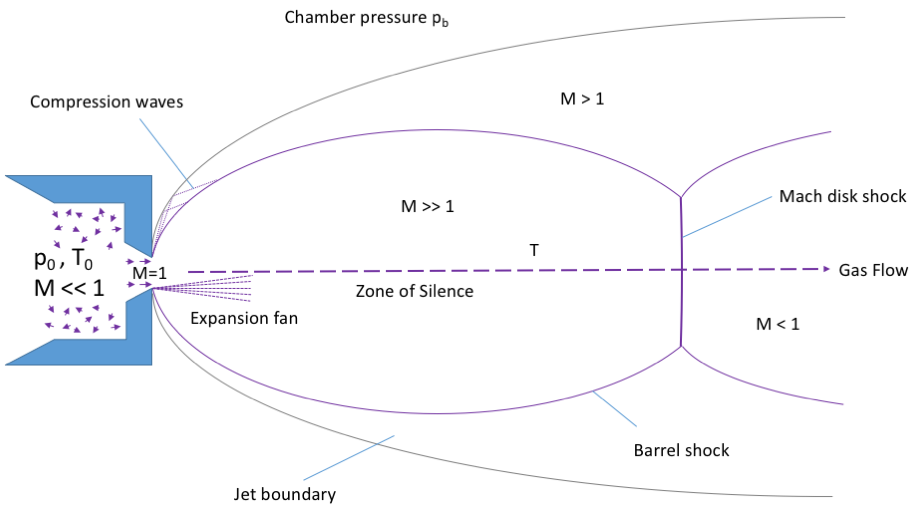
\includegraphics[width=1.00\textwidth]{images/freeJetExpansion.png}
	\caption[Schematic of a supersonic gas expansion into a vacuum.]{Schematic of a supersonic gas expansion into the vacuum. Gas is stored in a reservoir at pressure $p_{0}$, temperature $t_{0}$ and speed of the gas is thermal distributed $\left(M\ll 1\right)$. As the gas enters the nozzle area, it is accelerated to the speed of sound $\left(M=1\right)$ and as the gas expands, the temperature T drops altering the speed of sound such that the gas now travels supersonic $\left(M\gg 1\right)$. In this expansion, clusters are generated in the nozzle region, where $M=1$ (see text for details). After \citep{Miller-1988-Oxford}.}
	\label{fig:freeJetExpansion}
\end{figure}
Supersonic jet setups typically store gas in a reservoir at a certain stagnation pressure $p_{0}$ and temperature $T_{0}$. The gas expands through a nozzle into a vacuum and figure \ref{fig:freeJetExpansion} shows a schematic drawing of this process. Typical values for $p_{0}$ are 10 bars, where the mean free path of the atoms is much smaller than the nozzle diameter D. This is why many collisions occur during the expansion in the nozzle and the above described kinetic theory explains the cluster formation. However, this holds not true in the supersonic molecular flow region, where no further cluster growth happens. To understand the expansion process in detail, we assume to work with an ideal gas and to describe the gas expansion itself, we further assume that no clusters are formed and that turbulence and effects of heat conduction are unimportant \cite{Yamada-2001-SciDir,Haberland-1994-Springer}.\\
To begin, the velocity distribution of the gas is thermally distributed at a set temperature $T_{0}$. The movement direction of each atom is randomly orientated. For an ideal gas, we can define the enthalpy $H_{0}$ in the stagnation chamber
\begin{align}
H_{0}=c_{p} T_{0},
\intertext{with the specific heat $c_{p}$ for atoms}
c_{p}=\frac{5}{2}k_{B},
\label{eq:stagnation-enthalpy}
\end{align}
where is the Boltzman constant $k_{B}$. The expansion of the gas through the nozzle is driven by the pressure difference $p_{vac}/p_{0}$. In the nozzle, the (steady) gas flow becomes directed and the enthalpy $H_{0}$ is converted into kinetic energy $\frac{1}{2}m v^{2}$ and a rest enthalpy $H$. So, in the expansion process, we can use the conservation of energy, and equation \eqref{eq:stagnation-enthalpy} we can write down
\begin{equation}
H_{0}=H+\frac{1}{2}m_{gas} v^{2} = c_{p}T+\frac{1}{2}m_{gas}v^{2},
\label{eq:local-temperature}
\end{equation}
with $T$ being the local temperature along the gas flow and $m_{gas}$ the atomic mass of the gas. To look at this in greater detail, let us define the Mach number $M$ as the ratio of the stream velocity $v$ and the local speed of sound $c_{s}$
\begin{equation}
c_{s}=\sqrt{\frac{\gamma k_{B} T}{m_{gas}}}.
\label{eq:local-speed-of-sound}
\end{equation}
With the ratio of specific heats $\gamma = \frac{c_{p}}{c_{v}}$ at constant pressure and volume, they can be regarded as independent of temperature for atomic gases, we can rearrange equation \ref{eq:local-temperature} to 
\begin{equation}
T=T_{0}\left(1+\frac{1}{2}\left(\gamma - 1\right)M^{2}\right)^{-1}.
\label{eq:local-temperature-definition}
\end{equation}
Here the interplay between the Mach number $M^{2}$ and the local temperature $T$ give insight into the directed mass flow versus the remaining thermal energy in the system. As indicated the the figure \ref{fig:freeJetExpansion}, M increases dramatically along the expansion axis and that is due to decrease in speed of sound $c_{s}$ that is proportional to $\sqrt{T}$ as indicated in equation \eqref{eq:local-speed-of-sound}. The gas quickly reaches the terminal velocity $v_{\infty}=\sqrt{\frac{2 R}{m_{gas}}\left(\frac{\gamma}{\gamma-1}\right) T_{0}}$, with $R$ being the universal gas constant, while the speed of sound is decreasing. This can be abused to calculate flight times $t_{\text{flight}}=\frac{d}{v_{\infty}}$, if the distance $d$ from nozzle to interaction point is known (see sub-section \ref{sec:jet-timing}). Finally, the expansion speed of the gas gives the name to such types of gas sources, namely supersonic jets.\\
Let us describe the appearance of the jet stream (see figure \ref{fig:freeJetExpansion}) next. Upon exiting the nozzle, the Mach number increases by a wide margin ($M\gg 1$), that means that the gas travels faster than information in this medium. Here, a \textit{zone of silence} is formed, where the gas flow is not influenced by other particles, thus uninterrupted. As the supersonic flow is exiting the nozzle it has to turn around the edge of the nozzle to further expand and the supersonic flow turns by actually creating smaller Mach waves. At the borders of the \textit{zone of silence}, $M$ decreases drastically resulting in dense regions that are called \textit{barrel shock} to the sides and \textit{Mach disk} downstream the gas flow. For an unhindered transport of the gas and clusters to the interaction region, the interaction region needs to be within the \textit{zone of silence}. We can express the distance from the nozzle to the Mach disk $x_{MD}$ through
\begin{equation}
\frac{x_{MD}}{d}=0.67\sqrt{\frac{p_{0}}{p_{b}}},
\label{eq:distance-of-mach-disk}
\end{equation}
with the nozzle diameter $d$. So the competing stagnation pressure $p_{0}$ and the background pressure $p_{b}$ define the distance of the otherwise static parameters. $p_{b}$ needs to be low enough do drive the Mach disk downstream of the interaction region. By using skimmers and thereby physically separating the jet expansion into separately pumped compartments, the background pressure $p_{b}$ can be reduced, hence $x_{MD}$ increased.\\
While we have described a cooling gas in the expansion process it should be noted that the clusters are comparably hot. Through the kinetic process described above, they are efficiently heated. The two processes to loose energy are, one, collisions with a chaperone $M$ that deactivates the cluster, or two, evaporation of monomers from the cluster. The evaporation process makes the temperature size-independent, after the clusters have reached a certain minimum size \cite{Farges-1981-SurfSci}. Typically, the jet reaches temperatures of a few Kelvin and the cluster temperature is heavily dependent on their material, particularly the dissociation energy. For this study relevant are mostly the temperature of Xenon cluster that is $~75K$\footnote{To put this temperature in perspective, krypton clusters are $~50K$ and argon cluster $~40K$ \citep{Farges-1981-SurfSci,Gspann-1986-Springer}. Note that in this study the cluster size was $\bar{N} > 800$, hence above the minimum value to be size independent. For the evaporative cooling process to settle at a given temperature, a certain flight distance (in the cited study 6.5cm) should also be taken into account.} and the fact xenon clusters are solid as their melting temperature is higher \cite{Gspann-1986-Springer}. For similar reasons, helium clusters are liquid, which is why they are often called (helium-)droplets. If helium droplets are produced using a cryogenic jet even superfluid helium-droplets can be observed.\\
\begin{table}
	\centering
		\begin{tabular}{ | l | l | l | l | l | }
			\hline
			Helium & Neon & Argon & Krypton & Xenon \\ \hline
			3.85 & 185 & 1646 & 2980 & 5554 \\ \hline
		\end{tabular}
	\caption[Parameter $K_{\text{gas}}$ values for rare gases.]{Parameter $K_{\text{gas}}$ values for rare gases \cite{Schorb-2012-Thesis}.}
	\label{tab:k-parameter}
\end{table}
At the current point of the discussion, it should shine out that the average cluster size\index{cluster size} is very much depended on the gas type, stagnation temperature $T_{0}$, stagnation pressure $p_{0}$ and the nozzle type. Indeed, an empirically found scaling law\index{scaling law} named after Hagena\index{Hagena|see {scaling law}} \cite{Hagena-1972-JCP,Hagena-1981-SurfSci,Hagena-1987-ZeitschriftAMC}, can be written down as
\begin{equation}
\Gamma^{*} = K_{\text{gas}} \cdot T_{0}^{0.25q-1.5} \cdot p_{0} \cdot d_{eq}^{q}\quad \left[\frac{\text{$\mu$m mbar}}{\text{K}}\right],
\label{eq:Hagena-parameter}
\end{equation}
with the gas specific parameter $K_{\text{gas}}$ that can be found in table \ref{tab:k-parameter} for some rare gases, the gas specific parameter $q$ that varies between 0.5 and 1 and is 0.85 for all rare-gases, and the equivalent nozzle opening $d_{eq}$ that is $d_{eq}=d$ for pinhole sources and for conical nozzles $d_{eq}$ reads \citep{Schorb-2012-Thesis}
\begin{equation}
d_{eq} = d\frac{\tan\left(\Phi_{0}\right)}{\tan\left(\Phi\right)} = 0.719 \frac{d}{\tan\left(\Phi\right)}
\label{eq:equivalent-nozzle-opening}
\end{equation}
with the half opening angle of the nozzle $\Phi$ and the half opening of the free gas expansion $\Phi_{0}$. The Hagena scaling parameter $\Gamma^{*}$\index{Hagena!scaling parameter} allows us to estimate the mean cluster size, i.e. amount of accumulated particles per cluster $<N>$, as follows
\begin{itemize}
	\item $\Gamma^{*} < 350$, no cluster formation observed.
	\item $350 < \Gamma^{*} < 1800$, in this region $<N>$ reads
		\begin{equation}
		<N> = 38.4 \left(\frac{\Gamma^{*}}{1000}\right)^{1.64}
		\label{eq:intermediate-hagena-scaling}
		\end{equation}
	\item $1800 < \Gamma^{*}$, in this region $<N>$ reads
		\begin{equation}
		<N> = 33.0 \left(\frac{\Gamma^{*}}{1000}\right)^{2.35}
		\label{eq:large-hagena-scaling}
		\end{equation}
\end{itemize}
Supersonic jets generally create clusters of different sizes. This size distribution is centered around $<N>$ and for solid rare gas clusters this distribution is a log-normal distribution. The size distribution can be an experimental challenge, especially when size dependent effects are investigated. Historically, electron diffraction \cite{Farges-1981-SurfSci,Bartell-1986-ChemRev} has been used to determine the mean cluster size, mean temperature and mean geometry. Today, free electron laser allow the determination of the size of a single cluster through a diffraction image and by measuring enough single clusters, one can reproduce size distributions of a supersonic jet as shown in figure \ref{fig:size-distributions}.\\
Experiments using supersonic jets for cluster generation are typically performed with pulsed valves to decrease cost and gas load in the overall system. Upon opening and closing of the valve, the gas density varies. This mostly affects the cluster size and one would expect to see smaller clusters. This remains true in the beginning of the pulse but in the \textit{afterpulse}\index{afterpulse} one finds giant clusters that exceed the above described scaling laws due to the effects when closing the valve \cite{Rupp-2014-JCP}.
%
%
%
%
%
\subsection{Creation of heterogeneous cluster: The pickup principle}\label{sec:heterogeneous-cluster}
%%%%%%%%%%%%%%%%%
%- Heterogeneous clusters, e.g. He Xe\\
%- Do you have literature on that?
%%%%%%%%%%%%%%%%%
\begin{figure}
	\centering
		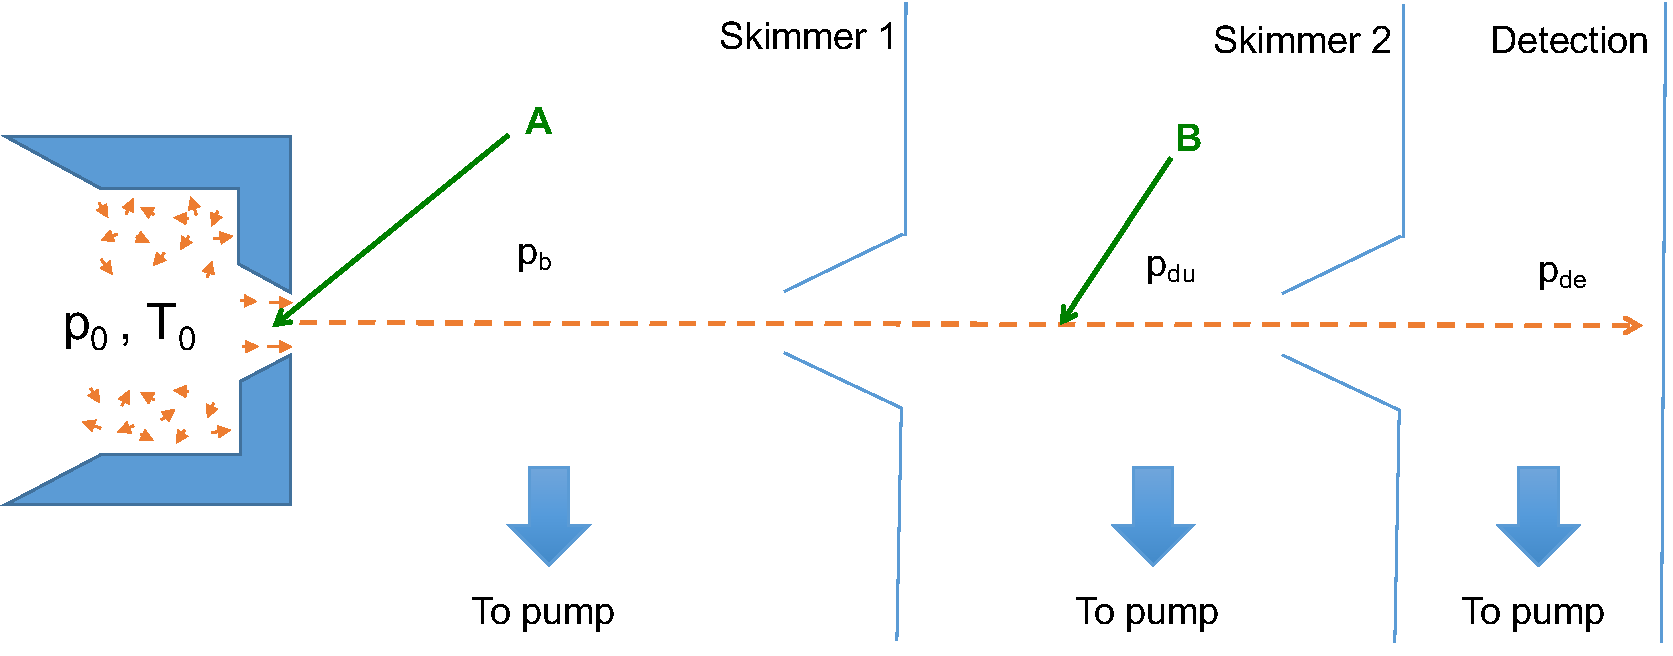
\includegraphics[width=0.80\textwidth]{images/pick-up.pdf}
	\caption[Schematic of a pickup (gas-)source.]{Schematic setup to generate heterogeneous clusters through pickup. Thereby is a cluster generated via supersonic gas expansion, which is doped at regions marked A or B. In region A, the dopant gas is mixed in the nozzle such that it becomes part of the nucleus. In region B, the cluster condenses atoms on its surface from the background gas of pressure $p_{\text{du}}$. The cluster can be detected upon evaporation, e.g., due to contact with the chamber, through the pressure $p_{\text{de}}$. After \cite{Gough-1985-JChemPhys,Haberland-1994-Springer}.}
	\label{fig:pickupPrinciple}
\end{figure}
A possibility to create heterogeneous clusters is through the principle of picking-up atoms or molecules \cite{Gough-1985-JChemPhys,Haberland-1994-Springer}. Figure \ref{fig:pickupPrinciple} illustrates pickup regions that are typically used in an experiment. Mainly, there are two different pickup places, one, monomers are added to the cluster in region A of figure \ref{fig:pickupPrinciple} that represents the nozzle of a supersonic source, or two, they can be picked up by a cluster in region B for example through an increased background pressure $p_{b2}$ with the dopant material. If clusters pick up atoms or molecules in the nozzle region A, they can become part of the cluster formation and can be found inside of solid clusters. If atoms or molecules are picked up in region B, they stick to the surface of solid clusters. If a (super-)liquid cluster picks up a dopant, it may move within the droplet. Since the traversing cluster is much larger and heavier than a colliding monomer the trajectory is not affected significantly. Already pressures of $p_{b2}=10^{-11}$ bars over a pickup length of a few centimeters can dope the cluster in significant form. At these low pressures, picking up atoms or molecules in region B requires less gas load on the system but is also less efficient than picking up in region B. To increase the pickup levels in region B, a gas cell can be used as much higher pressures can be achieved within the gas cell without putting too much gas-load on the overall system.\\
The collision with the cluster and a dopant\index{dopant} does add energy to the cluster just as the cluster growth process itself. This is why the initial cluster will loose particles through evaporation upon pick up of a dopant \citep{Gomez-2011-JCP}. The loss of particles through evaporative cooling is dependent on the ratio of dissociation energies of the two materials and can be written down as
\begin{equation}
N_{\text{Evaporated from cluster}} \approx \frac{\epsilon_{\text{cluster}}}{\epsilon_{\text{dopant}}},
\label{eq:evaporated-amount}
\end{equation}
with the dissociation energy of the cluster $\epsilon_{\text{cluster}}$ and of the dopant $\epsilon_{\text{dopant}}$. In the case, where a helium droplet is doped with xenon atoms, we may use the dissociation energies of helium $\epsilon_{He}=0.6\cdot 10^{-3}$ eV and xenon $\epsilon_{Xe}=0.6\cdot 10^{-3}$ eV \citep{Gomez-2011-JCP,Gomez-2014-Science}, such that approximately 250 helium atoms evaporate by picking up 1 xenon atom.\\
We can extend this idea to estimate the amount of picked-up atoms, if we were to know the amount of atoms in the cluster before and after the pickup area. An estimate of the initial cluster size $\left\langle N_{\text{cluster}}\right\rangle$ can be reached through the scaling laws\footnote{As already established the actual cluster size produced with a supersonic jet will vary, hence the average cluster size $\left\langle N_{\text{cluster}}\right\rangle$.} as discussed in section \ref{sec:homogenous-cluster}. A measure to estimate the cluster size after the pickup can be established through measuring the partial pressure of the cluster material $p_{\text{cluster}}$ of helium\footnote{For example with a residual gas analyzer.}, when the particle jet hits a wall and evaporates (see figure \ref{fig:pickupPrinciple}). The partial pressure $p_{\text{cluster}}$ then scales linearly with the initial cluster size $\left\langle N_{\text{cluster}}\right\rangle$, such that
\begin{equation}
\left\langle N_{\text{dopant}}\right\rangle \approx \frac{\epsilon_{\text{cluster}}}{\epsilon_{\text{dopant}}} \cdot \frac{\Delta p_{\text{cluster}} \left\langle N_{\text{cluster}}\right\rangle}{p_{\text{cluster}}},
\label{eq:average-dopant}
\end{equation}
where $\Delta p_{\text{cluster}}$ denotes the partial pressure difference between with pickup and without.
%%%
%\section{Introduction into X-ray scattering}\label{sec:scattering-theory}
%%%%%%%%%%%%%%%%%%%%%
%- Starting with Maxwell equations (this would be coming from the far end, I might be able to go into Guiniers formalism earlier. Depending on space.)\\
%- Mathematical model for electromagnetic wave\\
%- Kramers-Kronig relations\\
%- Mie scattering in a nutshell
%%%%%%%%%%%%%%%%%%%%%%%
%
\section{Soft X-rays in matter}\label{sec:light-matter-interaction}
We may break down the light-matter interaction into five categories, 1) coherent-elastic scattering (see sub-section \ref{sec:saxs}), 2) inelastic processes (absorption, see sub-section \ref{sec:absorption}), 3) incoherent scattering (Compton effect) and high-energy physics effects of 4) pair production and 5) absorption effects with the nucleus. The effects are dependent on the wavelength and the cross-sections for 3-5 can be neglected in the soft X-ray regime. We will therefore concentrate the following sections on points 1-2 and restrict ourselves to the for the experiment necessary theory.
%This section will give  a brief introduction into the elastic scattering of X-rays with matter. The actual scattering process is very complex as it is an interplay of coherent, incoherent and elastic, inelastic processes. Fortunately, we can reduce the scattering description to its main process: The coherent and elastic scattering. In other words, we neglect Compton scattering (incoherent), any kind of absorption processes (inelastic) and effects form the scattering of multiple particles. We will then start this section by looking at the small angle scattering of atoms and continue on to extended objects such as clusters. The section is rounded off by an introduction to the inverse problem and basic algorithm ideas to overcome the issue of phase retrieval.
%Photons can also be absorbed by atoms in which case an electron get either excited to another state or ionized. At X-ray wavelengths matter typically gets ionized in the inner shells. Upon absorption a cascade of relaxation processes begins and the now ionized atom finds the new most energetic favorable state. These processes are particularly depended on the wavelength of the incident photons but also the type of atom. This chapter is devoted to these processes and particular the absorption process is described in section \ref{sec:absorption} and the relaxation processes in \ref{sec:relaxation}.
%
%
%
\subsection{Small angle X-ray scattering}\label{sec:saxs}
%%%%%%%%%%
%- Switch to Guiniers approximation and description\\
%- Work towards small angle scattering of small particles\\
%- Particular spheres\\
%- Discuss extreme positions
%%%%%%%%%%%
We can describe a linear polarized, electric field of a continuous electromagnetic wave via the following expression \citep{Als-Nielson-2011-JWS}
\begin{equation}
\vec{E}(\vec{r},t) = \vec{\epsilon} E_{0} e^{i \vec{k}\cdot\vec{r}},
\end{equation}
with $\vec{E}(\vec{r},t)$ being the electromagnetic field of the wave, the wave vector $\vec{k}$, the Cartesian coordinate vector $\vec{r}$, the complex amplitude if the electric field is then $E_{0}\exp^{i \vec{k}\cdot\vec{r}}$ and because of the polarization we use $\vec{\epsilon}$ such that $\vec{\epsilon}\cdot\vec{k}=\vec{k}\cdot\vec{E}=\vec{k}\cdot\vec{H}=0$. Through a relative comparison, of the incoming intensity $I_{0}$ and the scattered intensity $I_{\text{sc}}$, we can phenomenological establish the differential cross-section over a certain solid angle $\Delta \Omega$ as
\begin{align}
\left(\frac{d\sigma}{d\Omega}\right)&=\frac{\left(\text{Number of X-rays scattered per second into $\Delta \Omega$}\right)}{\left(\text{Incident flux}\right)\left(\Delta\Omega\right)}=\frac{I_{sc}}{\left(I_{0}/A_{0}\right)\Delta\Omega},
\label{eq:scattering-crosssection}
\end{align}
with $A_{0}$ being the covered area of the incident beam. If an electro-magnetic wave encounters an electron, we can describe the scattering semi-classical by imagining how an electron starts to oscillate once it sees an incoming electric wave. The electron then functions as a dipole antenna eventually radiating the wave into a certain solid angle $\Delta \Omega$. Depending on the polarization of the incident beam we can reduce equation \ref{eq:scattering-crosssection} to \citep{Als-Nielson-2011-JWS}
\begin{align}
\left(\frac{d\sigma}{d\Omega}\right)&=r_{0}^{2}P,
\intertext{with the classical electron radius $r_{0}=2.82\ 10^{-5}\text{\AA}$ and the polarization factor P}
P&=\begin{cases}
1& \text{vertical scattering plane},\\
\cos^{2}\left(\Psi\right)&\text{horizontal scattering plane},\\
\frac{1}{2}\left(1+\cos^{2}\left(\Psi\right)\right)& \text{unpolarized source.}
\end{cases}
\end{align}
We can now move on and use this knowledge for atoms, where we have Z electrons. To describe electrons in an atom, let us proceed by introducing the electron density $\rho_{e}\left(\vec{r}\right)$ that describes the probability density of electrons in an atom. Figure \ref{fig:X-ray-scattering} illustrates the scattering process in one atom. An incident beam with wave number $\vec{k}$ is elasticly scattered at a point $\vec{r}$ into a wave with $\vec{k}'$ such that $\left|\vec{k}\right|=\left|\vec{k}'\right|$. In this wave picture, the scattering process must be seen as a superposition of waves and it is particular illustrated how the wave scattered at the origin of the atom is scattered as well. As both waves are scattered at different points, they have an optical path difference $2 \delta$. This difference in path length results in a phase difference to each other and eventually leads to interference between the waves. So, we can describe the phase difference $\Delta \Phi\left(\vec{r}\right)$ of the waves scattered at $\vec{r}$ and the origin by
\begin{equation}
\Delta \Phi\left(\vec{r}\right) = \left(\vec{k}-\vec{k}'\right)\cdot \vec{r} = \vec{Q} \cdot r,
\label{eq:phase-difference}
\end{equation}
with $\vec{Q}$ being denoted as the \textit{wave vector transfer}\index{wave vector!transfer}. Through trigonometry, we can establish the more common denotation of the wave-vector $\vec{Q}$
\begin{equation}
\vec{Q}=2 \left|\vec{k}\right| \sin\left(\frac{\Theta}{2}\right)=\frac{4 \pi}{\lambda}\sin\left(\frac{\Theta}{2}\right),
\label{eq:Q-scattering-angle}
\end{equation}
with the wavelength of the light $\lambda$ and the scattering angle $\Theta$.\\
A volume element $d\vec{r}$ at $\vec{r}$ will now scatter depending on its electron density, namely by $-r_{0}\rho\left(\vec{r}\right)d\vec{r}$. At scattering angle $\Theta=0$, i.e. $\vec{Q}=0$ the atomic scattering factor $f^{0}$ is
\begin{equation}
f^{0}\left(\vec{Q}\rightarrow 0\right)=Z,
\label{eq:transform-number-of-particles}
\end{equation}
because all scatterer are in phase. As we increase the scattering angle $\Theta$, the phase difference $\Delta \Phi\left(\vec{r}\right)$ leads to interference, which we can describe by multiplying a phase factor $e^{i \vec{Q}\cdot \vec{r}}$ to the electron density $-r_{0}\rho\left(\vec{r}\right)d\vec{r}$. In the limit of $\vec{Q}\rightarrow\infty$, the atomic scattering factor then is $f^{0}\left(\vec{Q}\rightarrow\infty\right)=0$. We can integrate over the total scattering length, and write down
\begin{equation}
-r_{0} f^{0}\left(\vec{Q}\right)=-r_{0}\int\rho_{e}\left(\vec{r}\right)e^{i \vec{Q}\cdot \vec{r}}d\vec{r}.
\label{eq:scattering-integral}
\end{equation}
\begin{figure}
	\centering
		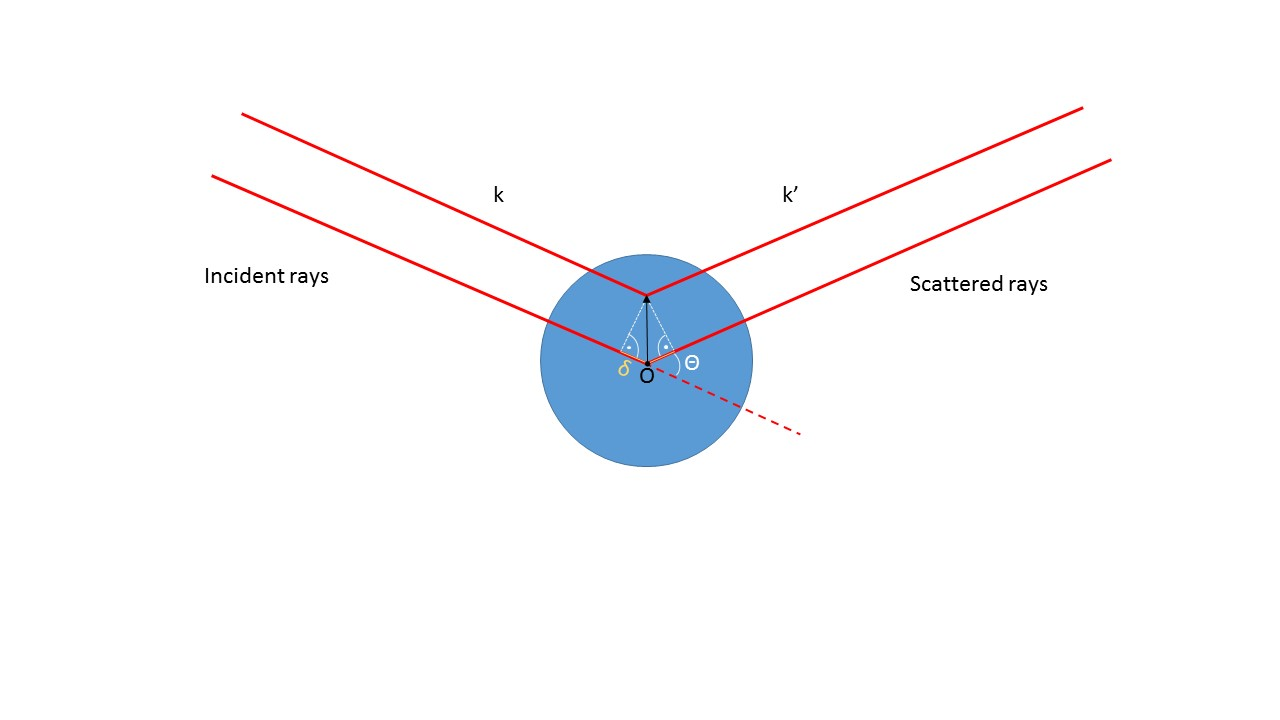
\includegraphics[width=1.00\textwidth]{images/X-ray-scattering.jpg}
	\caption[Principle of scattering rays of an atom.]{Principle of scattering rays of an atom. After \cite{Als-Nielson-2011-JWS,Guinier-1955-JWS}.}
	\label{fig:X-ray-scattering}
\end{figure}
This important result is called the atomic scattering factor in units of $-r_{0}$. It can be understood as a Fourier transform of the electron density of an atom.\\
Let us continue with the scattering of a molecule or cluster that consist of multiple atoms. We can label the atoms in such an object by
\begin{equation}
F^{object}\left(\vec{Q}\right)=\sum_{j}f_{j}^{O}\left(\vec{Q}\right)e^{i \vec{Q}\cdot \vec{r}},
\label{eq:scattering-factor-object}
\end{equation}
with the atomic scattering factors $f_{j}^{0}\left(\vec{Q}\right)$ for the $j$'th atom and call $-r_{0} F^{object}$ the scattering length of the object. Strictly speaking and as defined in \eqref{eq:scattering-factor-object}, $F^{object}\left(\vec{Q}\right)$ and $f_{j}^{Q}\left(\vec{Q}\right)$ is $\vec{Q}$ depended. As this is inconvenient, let us consider the following evidence in order to neglect this dependency. In the angular range of $\vec{Q}$, where $F^{Object}\left(\vec{Q}\right)$ is not 0, $f_{j}^{Q}$ can be considered constant \citep[see][p. 6-7]{Guinier-1955-JWS}. In human hemoglobin, the range in which the molecule scattering length $F^{Object}\left(\vec{Q}\right)$ is not 0, the carbon atomic form factors change less than $0.4$\%. Neglecting this $\vec{Q}$ dependency in $f_{j}^{Q}$ allows us to describe the scattering length of extended objects $F^{Object}\left(\vec{Q}\right)$ via one continuous electron density $\rho_{e}\left(\vec{r}\right)$, where certain volume elements $d\vec{r}$ scatter proportional to their electron density $\rho_{e}\left(\vec{r}\right)$. Let us write down the more convinient expression for the scattering length of an object
\begin{equation}
-r_{0}F^{O}=-r_{0}\int \rho\left(\vec{r}\right) e^{i \vec{Q}\cdot r}d\vec{r},
\label{eq:scattering-factor-general}
\end{equation}
and we can see that it is mostly the phase factor that yields information about the structure of the object as it is the phase factor that constitutes the diffraction pattern.\\
The total scattered intensity $I\left(\vec{Q}\right)$ in a diffraction pattern can expressed through
\begin{equation}
I\left(\vec{Q}\right)=\left|A\right|^{2}=I_{0}\left|F^{0}\left(\vec{Q}\right)\right|^{2},
\label{eq:scattered-intensity}
\end{equation}
where an incident beam with intensity $I_{0}$ with a complex amplitude $A$\index{amplitude!complex} performs an operation that can be interpreted as a Fourier transform of the objects electron density. The process of measuring the scattered light, for example through a detector, merely measures the modulo of an amplitude $\left|A\right|^{2}$, which eliminates the phase factor $e^{i\Delta\Phi\left(\vec{r}\right)}\cdot e^{-i\Delta\Phi\left(\vec{r}\right)}=1$. In order to reconstruct the object that scattered in realspace, e.g. to understand its shape or to study its function, we need to recover the for the structure most important phase information. We will discuss iterative algorithms that can recover phase information in section \ref{sec:phase-retrieval}.\\
Let us briefly address the scattering of a rare-gas cluster, as the cluster can be considered as a sphere alike object in sub-nanometer approximation\footnote{Considering experimental details from chapter \ref{ch:exp_setup}}. We can express the electron density of a simple sphere with radius $R$ as 
\begin{align}
\rho\left(\vec{r}\right)&=\begin{cases}
1& \text{for $R \geq \vec{r} \geq 0$},\\
0&\text{for $R > \vec{r}$}.
\end{cases}
\label{eq:el-density}
\end{align}
Using equation \eqref{eq:el-density}, we can solve the integral in equation \eqref{eq:scattering-factor-general} by transforming into spherical coordinates
\begin{align}
F_{\text{Sphere}}^{O}\left(\vec{Q}\right) &= \int_{0}^{\pi}\int_{0}^{2\pi}\int_{0}^{R} r^{2}  sin\left(\Theta\right) e^{i \vec{Q} r \cos\left(\Theta\right)} dr d\Theta d\Phi\\
&=\frac{\sin\left(\vec{Q} R\right)-\vec{Q} R\cos\left(\vec{Q} R\right)}{\vec{Q}^{3} R^{3}}=\frac{J_{1}\left(\vec{Q}R\right)}{\vec{Q}R},
\label{eq:scattering from sphere}
\end{align}
with $J_{1}$ being the Bessel function of first kind. Formula \eqref{eq:scattering from sphere} can be easily abused to determine the size of a spherical particle using local minima in the diffraction pattern\footnote{Equation \eqref{eq:scattering from sphere} can be solved numerically for the distance between the first two minima $\Delta\vec{Q}R=3.24$, such that $R=\frac{3.24}{\vec{Q}_{\text{min}^{n+1}}-\vec{Q}_{\text{min}^{n}}}$} or through a numerical fit of the resulting curve.
%
%
%\subsection{X-ray diffraction}
%- I wonder if I should include this to talk about 'what happens on faster timescales' using Ken's work.
%
%
%
%
\subsection{Ionization of matter}\label{sec:absorption}
Let us quickly remember the atomic scattering factor $f^{0}\left(\vec{Q}\right)$ that were introduced in the last section by neglecting a variety of (wavelength depended) effects through Fourier transforming the electron density of an atom. As we established, we can compare the photon-electron interaction to the analogue of the forced harmonic oscillator, where an electric field drives a (bound) electron. However, it is not only the light field that drives the electron, also the electron has an effect to the light field. As the wave propagates through a medium, the phase velocity of light $v_{\text{phase}}$ is slower than the speed of light in vacuum $c$ due to interacting with electrons. We can describe this effect via the refractive index $n\equiv c/v_{phase}$\index{refractive index}. Another aspect to consider is a reduction of the amplitude of the incoming electro-magnetic wave (absorption), when the energy of the photons is higher than the binding energies of electrons \citep{Als-Nielson-2011-JWS,Attwood-2007-CUP}. These two effects are connected to the atomic scattering factors $f^{0}\left(\vec{Q}\right)$ and are called dispersion corrections. Let us include these corrections to the atomic scattering factor and define the atomic form factor
\begin{equation}
f\left(\vec{Q},\hbar\omega\right)=f^{0}\left(Q\right)+f'\left(\hbar\omega\right)+i f''\left(\hbar\omega\right),
\label{eq:scattering-factor-dispersion-corr}
\end{equation}
where $f'\left(\hbar\omega\right)$ corrects for the phase velocity and the wave amplitude correction/absorption $f''\left(\hbar\omega\right)$. In the limit of high photon energies $\hbar \omega$, bound electrons can be largely seen as free, as the binding energies become a little factor, therefore $f'\left(\hbar\omega\right)\rightarrow 0$ and $f''\left(\hbar\omega\right)\rightarrow 0$. As the photon energies $\hbar \omega$ are closer to the atomic level, which is the case at soft X-rays for many materials, $f'\left(\hbar\omega\right)$ and $f''\left(\hbar\omega\right)$ can become large factors.\\
We shall not derive this topic in its full extend as it can be found in \citep[][p. 55 ff]{Attwood-2007-CUP}, but we shall qualitatively compare the equation for the complex refractive index $n\left(\omega\right)$ to the previous considerations about the forced harmonic oscillator. For simplicity, we reduce the following considerations to the case of forward scattering, where $\vec{Q}=\Theta=0$.\\
Imagine a electromagnetic wave propagating in a medium. The wave propagating in a medium along the axis $z$ can be written as
\begin{equation}
e^{i n k z}= \underbrace{e^{i \left(1-\delta\right)k z}}_{\text{phase shift}}\underbrace{e^{-\beta z}}_{absorption},
\label{eq:wave-in-medium}
\end{equation}
\begin{figure}
	\centering
		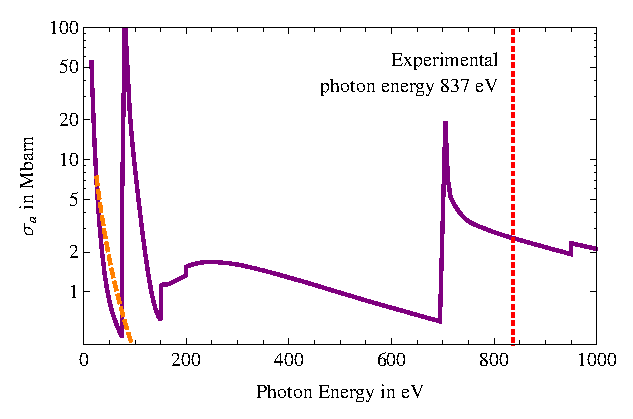
\includegraphics[width=0.80\textwidth]{images/photoionization.eps}
	\caption[Total absorption cross-sections for helium and xenon.]{Total absorption crosssections $\sigma_{a}$ in megabarn for xenon (purple line) and helium (orange dashed). The photon energy of the described experiment is $\sim 837$ eV (red dashed). Data points from \citep{Elettra-2016-Website,Yeh-1985-AtmDat,Yeh-1993-GBSP}}
	\label{fig:photoionization}
\end{figure}
where $n$ is the complex refractive index, $\delta$ the real dispersion correction\index{dispersion correction!complex} resulting in a phase shift of the wave and $\beta$ being the imaginary dispersion correction resulting in a decline in amplitude of the wave\footnote{We jump between wave and particle picture as it pleases us. Here, a decline in amplitude in the wave picture can be read as absorption in the particle picture.}. The relation between the complex refractive index $n$, $\beta$ and $\delta$ is explicitly given by
\begin{equation}
n\equiv \frac{c}{v_{\text{phase}}}=1-\delta+i\beta.
\label{eq:complex-refractive-index}
\end{equation}
We can compare this equation \eqref{eq:complex-refractive-index} to equation \eqref{eq:scattering-factor-dispersion-corr} and realize that we are allowed to define this dispersion relation through the atomic form factor as \citep[see][p.~76]{Als-Nielson-2011-JWS}
\begin{equation}
n\equiv 1- \frac{2\pi \rho_{atom}r_{0}}{k^{2}}\left(f^{0}\left(\vec{Q}=0\right)+f'\left(\hbar\omega\right)+i f''\left(\hbar\omega\right)\right),
\label{eq:eq:complex-refractive-index-atomic-factors}
\end{equation}
with the atomic number density $\rho_{atom}$ and we identify explicitly
\begin{align}
\delta &= \frac{2 \pi \rho_{atom} r_{0}}{k^{2}}\left(f^{0}\left(\vec{Q}=0\right)+f'\left(\hbar\omega\right)\right),\quad \text{and}\\
\beta &= - \left(\frac{2\pi \rho_{atom}r_{0}}{k^{2}}\right)f''\left(\hbar\omega\right).
\label{eq:delta-and-beta}
\end{align}
We have already established in equation \eqref{eq:wave-in-medium} that $\beta$ reduces the amplitude of the incoming wave through absorption. Using this insight about absorption, we can rewrite equation \eqref{eq:delta-and-beta} and define $f''\left(\hbar\omega\right)$ in terms of being proportional to an absorption cross section $\sigma_{a}$, which reads
\begin{equation}
f''\left(\hbar\omega\right)=-\left(\frac{k}{4\pi r_{0}}\right)\sigma_{a}.
\label{eq:f-2-definition}
\end{equation}
Figure \ref{fig:photoionization} shows the total absorption cross-sections $\sigma_{a}$ for xenon, helium at which a bound electron absorbs a photon and excited into the continuum, thus the atom is ionized\index{photoionization}. To get a better understanding of the fundamental absorption related details about xenon and helium, table \ref{tab:xenon-photoionization-cross-section} and \ref{tab:helium-xenon-ionization} show the differential photo-absorption cross sections and ionization potentials for various energy levels and ionization configurations at the photon energy $837$ eV. The calculations were performed with the Los Alamos Atomic Physics code based on \citep{Cowan-1981-Cal}.
\begin{table}
	\centering
		\begin{tabular}{ | c | c | c | c | }
			\hline
			Shell & Subshell & Cross-section & subshell ionization \\
				&	& in Mb & potential in eV \\ \hline
			K & 1s & - & 34630.0 \\ \hline
			L & 2s & - & 5466.4  \\ 
			\ & 2p & - & 4899.1 \\ \hline
			M & 3s & - & 1153.3  \\ 
			\ & 3p & - & 965.4 \\ 
			\ & 3d & 2.2505 & 682.7 \\ \hline
			N & 4s & 0.0305 & 223.7 \\ 
			\ & 4p & 0.1247 & 161.8 \\ 
			\ & 4d & 0.2587 & 68.2  \\ \hline
			O & 5s & 0.0040 & 27.3  \\ 
			\ & 5p & 0.0120 & 12.5  \\ \hline
		\end{tabular}
	\caption[Differential absorption cross-sections and ionization potentials for xenon.]{Differential absorption cross-sections and ionization potentials for certain electronic configurations of xenon at 837eV. Calculations based on \citep{Cowan-1981-Cal}.}
	\label{tab:xenon-photoionization-cross-section}
\end{table}
It appears that certain energy levels, or here subshells if one disregards the hyperfine structure\footnote{A shift in energy levels due to interaction of electrons with the nucleus \citep[see][p~166~ff.]{Demtroder-2005-Springer}.}, tend to have a higher absorption cross-section than others. This brings us back to the picture of the forced harmonic oscillator, where an electron is driven by a light field. If the frequency of the light field is close to the eigenfrequency of the bound electron, in other words, if the energy of a photon is close to the energy level of a bound electron, the system is in resonance and absorption is highly likely. As the photon energy and electron level energy differ, the system is off resonance and it is less likely to absorb a photon. As energy levels in atoms are discrete, electrons can only be excited from one energy level to another or need a certain (minimal) ionization energy\index{ionization!energy} to ionize an atom and excite an electron into the continuum. Therefore, the likelihood of a core-electron that is strongly bound being ionized is by far the most probable using X-rays.
\begin{table}
	\centering
		\begin{tabular}{ | c | c | c | c | }
		\hline
%			Configuration & ionized subshell & Cross-section (Mbarn) & Helium ionization potential in eV \\ \hline
			El. Configuration, & Ionization & Cross-section  & subshell ionization  \\
			and ionized subshell & of subshell & $\sigma_{a}$ in Mbarn & potential in eV \\ \hline
			He\textsuperscript{+0},\ 1s2 & 1s2 & 0.0007 & 24.4 \\ \hline
			He\textsuperscript{+1},\ 1s1 & 1s1 & 0.0005 & 54.4 \\ \hline
			Xe\textsuperscript{+0},\ 5p6 & 3d10 & 2.2505 & 682.7 \\ \hline
			Xe\textsuperscript{+1},\ 3d9 & 3d9 & 2.1487 & 733.6 \\ \hline
			Xe\textsuperscript{+1},\ 5p5 & 3d10 & 2.2443 & 693.7 \\ \hline
			Xe\textsuperscript{+2},\ 5p4 & 3d10 & 2.2390 & 705.9 \\ \hline
		\end{tabular}
	\caption[Absorption cross-sections and ionization potentials for xenon and helium]{Absorption cross-sections $\sigma_{a}$ and ionization potentials for certain electronic configurations, including certain ionization profiles. Calculations based on \citep{Cowan-1981-Cal}.}
	\label{tab:helium-xenon-ionization}
\end{table}
When a core electron gets ionized, the electronic structure changes and particular ionization energies and (absorption) cross-sections change. To discuss the parameters that are most applicable to this thesis, a comparison of the most probable transition at the photon energy 837eV is given for helium and xenon in table \ref{tab:helium-xenon-ionization}. The ionization energies change drastically, whether a core electron or a less tight bound electron is ionized. As per absorption cross-sections, helium can be considered transparent and xenon atoms have a much larger absorption cross-section. The amount of ionization configurations can become rather complex and the table shall give the reader merely a broad understanding of some likely configurations.\\
%Similarly to the estimate made in equation \eqref{eq:absorption-cross-section}, it is very unlikely for an atom to absorb more than two photons in one pulse of a free electron laser, which is why we only consider the most probably transitions here to get an understanding how the absorption cross-sections change.\\
% \begin{table}
% 	\centering
% 		\begin{tabular}{ | c | c | c | c | }
% 		\hline
% 			El. Configuration, & Ionization & Cross-section  & subshell ionization  \\
% 			and ionized subshell & of subshell & $\sigma_{a}$ in Mbarn & potential in eV \\ \hline
% 			Xe\textsuperscript{+0},\ 5p6 & 3d10 & 2.2505 & 682.7 \\ \hline
% 			Xe\textsuperscript{+1},\ 3d9 & 3d9 & 2.1487 & 733.6 \\ \hline
% 			Xe\textsuperscript{+1},\ 5p5 & 3d10 & 2.2443 & 693.7 \\ \hline
% 			Xe\textsuperscript{+2},\ 5p4 & 3d10 & 2.2390 & 705.9 \\ \hline
% 		\end{tabular}
% 	\caption{caption. Calculations based on \citep{Cowan-1981-Cal}.}
% 	\label{tab:xenon-ionization}
% \end{table}{}
The total atomic scattering factors $f^{0}$ for neutral and ionized, helium and xenon can be found in table \ref{tab:helium-xenon-el-scattering-crossection}. It is interesting to see that although a xenon atom has only 27 times more electrons than a helium atom the scattering factor $f^{0}$ of neutral xenon is over 900 times stronger than helium. Upon ionization, the absolute changes in $f^{0}$ of helium are therefore smaller compared to xenon. The relative change in helium of $f^{0}$ after one electron is ionized is ~75\%, thus (ionized) helium barely scatters. As xenon has multiple occupied subshells, the scattering factors of different ionized subshells are shown in table \ref{tab:helium-xenon-el-scattering-crossection}. As discussed, it is most likely to ionize the xenon 3d subshell, however, within a few femtoseconds subsequent relaxation processes\footnote{See the following section \ref{sec:relaxation}.} lead to different ionization configurations, for example a double ionized 5p subshell. For the scattering factor, there is little change whether the 3d or 5p subshell becomes ionized and the change in $f^{0}$ is only ~0.05\%. As xenon has 54 electrons, the relative change upon ionization of one electron in $f^{0}$ is only 3\%. Xenon is therefore a much stronger scatterer than helium and xenon still scatters well upon ionization of inner or outer shell electrons.  
\begin{table}
	\centering
		\begin{tabular}{ | c | c | }
		\hline
			El. Configuration, & Scattering factor \\
			and ionized subshell & $f^{0}$ in barn \\ \hline
			He\textsuperscript{+0},\ 1s2 & 2.5539  \\ \hline
			He\textsuperscript{+1},\ 1s1 & 0.649465  \\ \hline
			Xe\textsuperscript{+0},\ 5p6 & 1874.36  \\ \hline
			Xe\textsuperscript{+1},\ 3d9 & 1813.56  \\ \hline
			Xe\textsuperscript{+1},\ 5p5 & 1814.68  \\ \hline
			Xe\textsuperscript{+2},\ 5p4 & 1754.08  \\ \hline
		\end{tabular}
	\caption[Atomic scattering factors for helium and xenon.]{Atomic scattering factor $f^{0}$ for certain electron configurations. Calculations based on equation \eqref{eq:scattering-integral}. From \cite{Ho-2016-PC}.}
	\label{tab:helium-xenon-el-scattering-crossection}
\end{table}
In the experiment described in the following chapters, the photon energy is explicitly chosen to have a comparably high absorption cross-section for xenon but is off absorption resonance, a comparably low absorption cross-section for helium and a wavelength short enough to receive high resolution images through coherent diffraction imaging. In such a setting xenon is most likely to absorb X-rays and helium can be considered as transparent. Furthermore, xenon acts as the strong scatterer when compared to helium.
%
%
%
%
%
\subsection{Charge migration}\label{sec:relaxation}
%%%
\begin{figure}
	\centering
		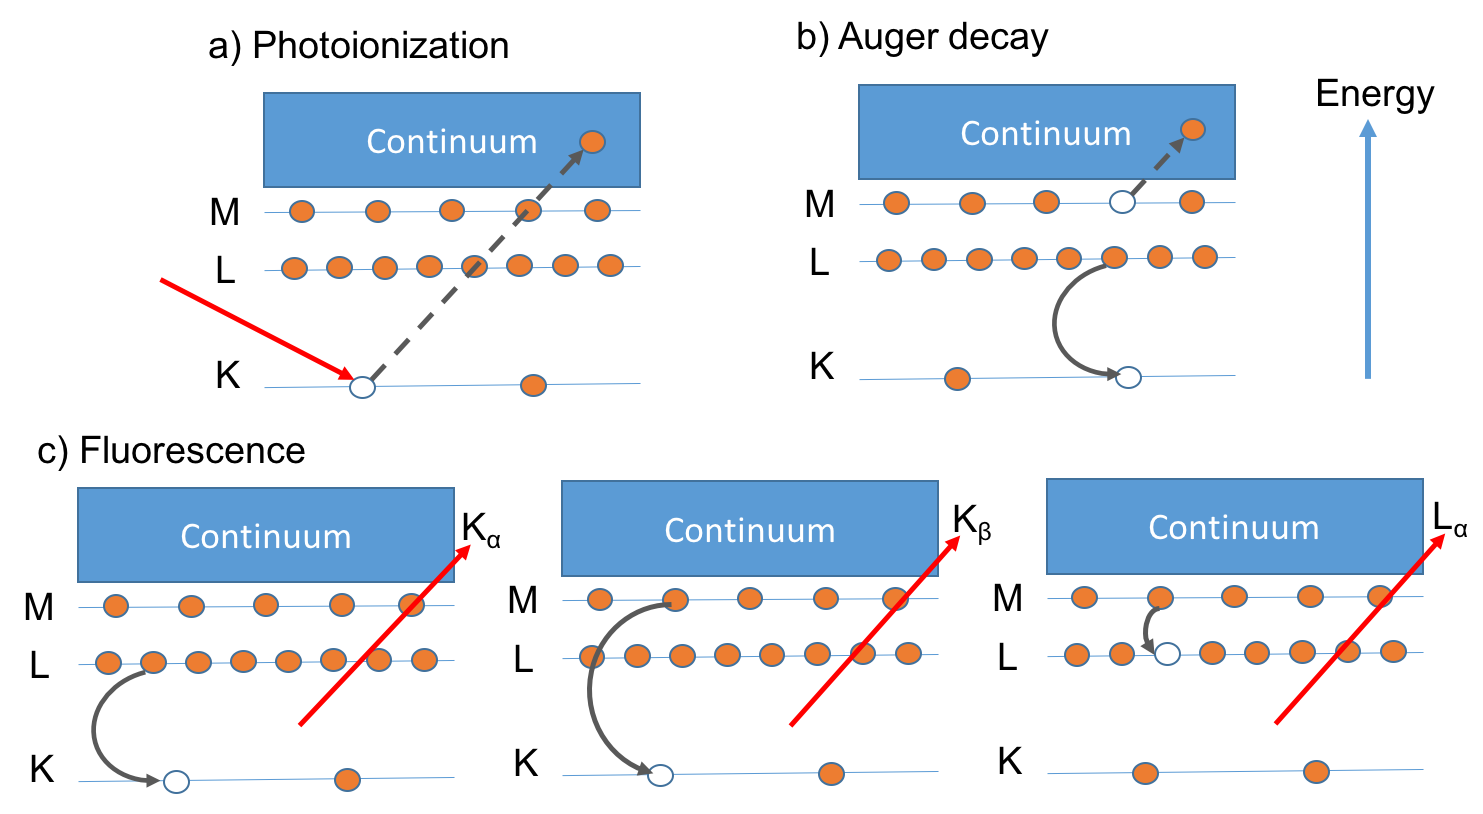
\includegraphics[width=0.80\textwidth]{images/el-relaxation.png}
	\caption[Schematic illustration of common charge transfer processes]{Schematic illustration of common charge transfer processes. a) photoionization: Describes a direct emission of a K-shell electron after absorbing a X-ray photon. b) Auger decay: A relaxation process, where a K-shell hole is filled with an electron from the L-shell and the remaining energy is released through emission of an electron in an outer shell. c) Fluoresence:An electron hole is filled with an electron from an outer shell and the remaining energy is released through photons. After \citep[][p.~19]{Als-Nielson-2011-JWS}.}
	\label{fig:el-relaxation}
\end{figure}
After an atom has been (core-)ionized due to absorption of a photon as depicted in figure \ref{fig:el-relaxation}a, the atom is usually not in its most energetically favorable state. In order to emit energy and transition into its new ground state, the atom can emit particles according to the schematics in figure \ref{fig:el-relaxation}b-c. In a fluoresence decay (\ref{fig:el-relaxation}c), the electron hole in the (K-)shell is filled by an electron in an energetically higher shell, here L or M shell, and thereby emits a photon of the discrete energy difference between the transitioning levels. If one spectrally resolves the discrete peaks are element specific and modern photoemission spectroscopy can yield insight into for example element identification, excitation dynamics or chemical bonds.
\begin{figure}
	\centering
		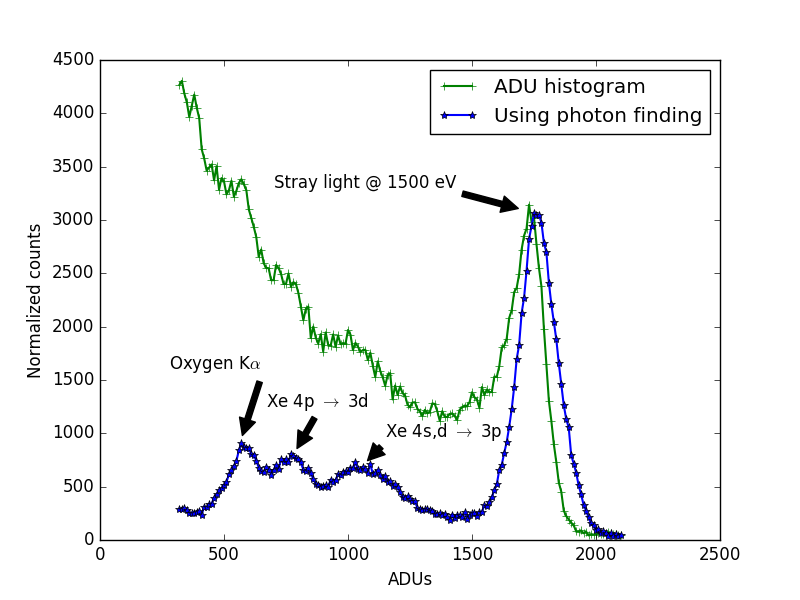
\includegraphics[width=.49\textwidth]{images/pnCCD-histogram.png}
		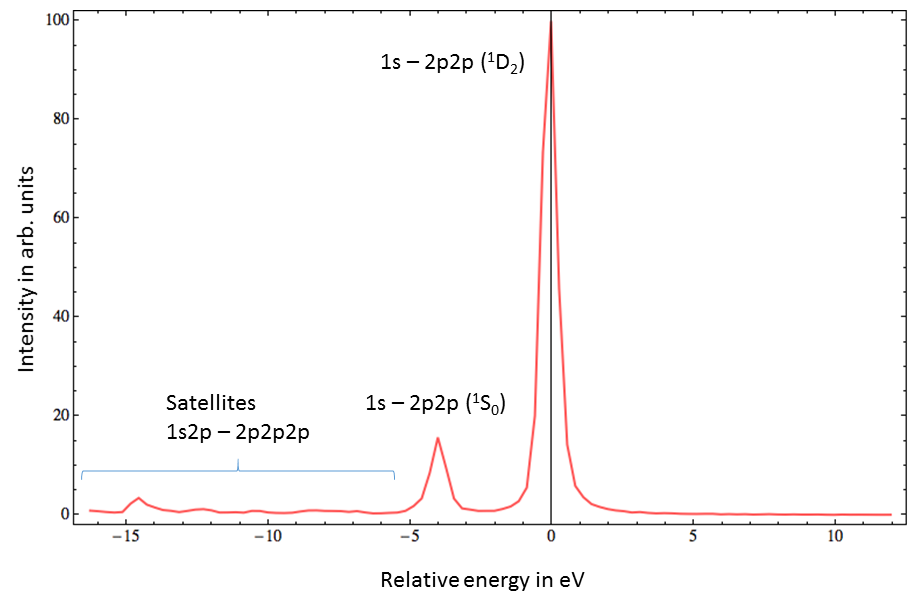
\includegraphics[width=.49\textwidth]{images/auger-spectra.png}
	\caption[Fluorescence spectra from xenon and neon K-LL Auger spectrum.]{Left spectra shows fluorescence peaks from xenon and oxygen illuminated with 1.5keV photons from the LCLS; detected with pnCCD detectors \citep{Bucher-2016-Unpublished, Rudek-2012-NatPho}. The green curve is an ADU histogram of the pnCCD detector and the blue curve uses a coalescent photon finder. Right, partial K-LL Auger spectrum with rel. energy 0 corresponding to 804.5 eV. Spectrum measured with photoelectron spectrometer \cite{Bucher-2014-Unpublished}, peaks identified as in \citep{Krause-1970-PhysLettA}.}
	\label{fig:pnCCD-histogram}
\end{figure}
Figure \ref{fig:pnCCD-histogram} left shows measured fluorescence lines of oxygen and xenon. In this measurement, xenon atoms and residual oxygen atoms have been illuminated with 1500 eV photons from the Linac Coherent Light Source and the fluorescence photons have been measured with the LAMP pnCCD detectors that are described in section \ref{sec:pnCCD}. The green curve is a ADU histogram of the pixel-detector using the detector calibrations described in section \ref{sec:pnccd-corr}. The blue curve additionally uses a photon-finding algorithm as the signal from just one fluorescence photon splits up into multiple pixel. The coalescent-photon finding algorithm\index{algorithm!coalescent-photon finding} looks for pixel above a certain threshold and includes neighboring pixel above a certain threshold, thus correcting the measured signal to yield a proper ADU count per photon.\\
%
The Auger decay is another possibility for the atom to emit energy through a 2-step process. One, an outer shell electron is emitted into the continuum, the so called Auger-electron\footnote{Named after the french physicist Pierre Auger.}. Two, another electron in the atom simultaneously fills the electron-hole. An Auger decay occurs typically on the few femtosecond timescale after ionization \citep{Krause-1970-PhysLettA}. Emitted Auger-electrons have discrete energies depending on the combination of electrons involved in the process. Similar to fluorescence spectroscopy, one can use this attribute to, for example, identify elements or calibrate energies. Figure \ref{fig:pnCCD-histogram} right shows a partial K-LL\footnote{This nomenclature means a single hole in the K-shell is followed by a two holes in the L shell after the Auger decay.} Auger spectrum from neon illuminated by 1050 eV photons from the LCLS and measured with a hemispherical analyzer as described in \citep{Bucher-2014-Unpublished}. In this example, neon is ionized in the K-shell and an electron-hole in the 1s shell is created. An electron from the L-shell fills the 1s hole and another electron from the L-shell, the Auger electron, is emitted into the continuum. As there is a variety of electronic configurations that can be involved in this process multiple peaks appear for similar occupation configurations, e.g. 1s - 2p2p. More complex structures, called satellites, appear when the atom is already ionized, for example, the atom has a hole in the L-shell and then an absorption that creates another hole in the K-shell. This will lead to KL-LLL satellites.\\
Similar to the Auger decay, where electrons from an outer shell are involved in the relaxation process, the transition can also be of the same shell and is then called a Coster-Kronig transition. Relevant transitions are for example the N-NN Coster-Kronig transitions in xenon \citep{Coster-1935-Physica}.
%\\So far we have looked at X-ray induced processes from atoms. Extended objects, whether a bio-molecule or a cluster, will respond differently than just the atoms they consist of. Nanometer-sized objects will develop a distinct character due to their electronic bond with other particles. This includes rare-gas clusters that are weakly bound Van der Waals forces. We shall explore this behavior in the next section \ref{sec:ionizatin-of-ext-obj}.
%
%
%
%
\section{Ionization of clusters in intense X-ray pulses}\label{sec:ionizatin-of-ext-obj}
%%%%%%%%%%%%%%%%%%%
%- Short introduction coming from inelastic scattering
%%%%%%%%%%%%%%%%%%%
Cluster have a long history as a testbed sample to investigate light-matter interaction. The response of a cluster upon irradiation with light often differs from just the atomic response. Collective effects change the (microscopic) sample environment and it is now the collective of atoms that generate a response to the interacting light. Clusters provide therefore a testbed environment to study collective effects ranging from atomic, to molecular and to bulk material attributes. While we went over some benefits of using clusters in section \ref{sec:cluster-theory}, it shall also be said that they provide an ideal testbed sample to control light-driven many-particle processes \citep{Fennel-2010-RMP}. In this section, we study how rare-gas cluster respond to femtosecond long, high intense X-ray pulses and reflect on recent experiments.
%
%
%
\subsection{Formation and expansion of a nanoplasma}\label{sec:nanoplasma-expansion}
%%%%%%%%%%%%%%%%%%%%%%%%
%- Step by step explanation on the formation of a nanoplasma
%%%%%%%%%%%%%%%%%%%%%%%%
\begin{figure}
	\centering
		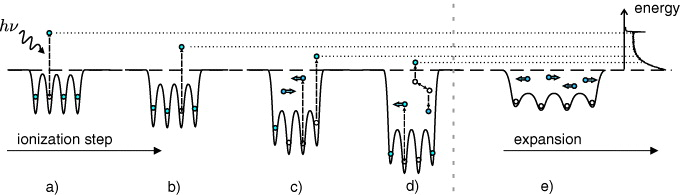
\includegraphics[width=1.00\textwidth]{images/nano-plasma-schematic.jpg}
	\caption[Schematic of the nanoplasma creation and expansion.]{Schematic of the nanoplasma creation and expansion. In step a) X-ray photons ionize electrons from a cluster. b) subsequent \textit{multistep ionization}\index{ionization!multistep} try to relax the electronically excited system, deepening the Coulomb potential of the cluster. Step c) shows a deepened Coulomb potential of the cluster, due to which the multistep ionization becomes (partially) frustrated and electrons are trapped in the potential. In step d) trapped electrons collide and start to thermalize. Collisions can lead to emission of trapped electrons. d) The superheated nanoplasma starts to expand. From \citep[\href{https://creativecommons.org/licenses/by/3.0/}{\ccby}]{Arbeiter-2011-NJP}}
	\label{fig:nano-plasma-schematic}
\end{figure}
 Let us recapture the elastic, coherent scattering part of the response that has been discussed in sub-section \ref{sec:saxs}. Equation \eqref{eq:scattering-factor-object} indicates how the scattering length of a cluster can be calculated and, even though we neglect inelastic processes, this response is close to actual measured scattering patterns. If, however, we consider the inelastic effects discussed in section \ref{sec:absorption}, it should be clear that the elastic scattering length -$r_{0}F^{Object}$ is reduced due to the (atomic) dispersion corrections $f'\left(\omega\right)$ and $f''\left(\omega\right)$ that reduce the scattering length $-r_{0}f^{0}\left(\vec{Q}\right)$ of a single atom. On the one hand, the dominating change in scattering length is driven by the absorption process that we introduced via the imaginary dispersion correction $i f''\left(\omega\right)$ but we know from table \ref{tab:helium-xenon-el-scattering-crossection} that the changes in scattering cross-section are relatively small. On the other hand, there are X-ray induced effects that change the scattering behavior of clusters. We know from previous experiments \citep{Gorkhover-2016-NatPho} that these changes are related to the nanoplasma expansion. Let us follow figure \ref{fig:nano-plasma-schematic} and \citep{Arbeiter-2011-NJP,Bostedt-2010-JPB} in the next five steps to get a better understanding of the nanoplasma phase-transition. Step a) of the nanoplasma transition\index{nanoplasma!transition}, the cluster gets ionized due to intense radiation\footnote{The wavelength of radiation must be above the ionization threshold of at least one subshell, however, it must not be X-rays with a wavelength on the nanometer length scale.}. Step b), further ionization through emission of photo electrons and Auger electrons lead to a so called \textit{multistep ionization}\index{ionization!multistep} that steepens the Coulomb potential\index{Coulomb potential} \citep{Wabnitz-2002-Nature,Laarmann-2004-PRL,Bostedt-2008-PRL}. Step c), the multistep ionization is suppressed (or frustrated) because the Coulomb potential depth is larger than the atomic excess energy of photo- and Auger electrons. The emitted electrons are now trapped in the cluster potential and are \textit{quasi-free}. Upon increasing \textit{inner ionization}\index{ionization!inner}, the nanometer sized object undergoes a phase transition to a nanoplasma\footnote{Plasma is another state of matter, similar to solid, liquid and gaseous, where molecular bonds dissociate and positive and negative particles are present in increasing numbers.}. Step d), the temperature of the nanoplasma is initially defined by the atomic excess energies (a rather discrete spectrum) but collisions with other particles lead a (kinetic) energy distribution of the electrons that is similar to thermal distributions and can be measured via the spectra of evaporated electrons \citep{Laarmann-2005-PRL,Bostedt-2010-NJP}. Step e) Hydrodynamic and Coulomb forces drive an expansion of the cluster and the cluster will ultimately disintegrate. The hydrodynamic portion of the force is due to the increasing hot plasma and the resulting increase outward pressure, whereas the Coulomb portion comes from the repelling force of same charges. Both forces reasonably describe the expansion process, are not mutually exclusive and depend mostly on sample size and irradiation technique.\\
Regarding the sample size, large clusters efficiently trap electrons in their Coulomb potentials such that the quasi-free electrons thermalize and subsequently heat the nucleus. The hot nanoplasma system then tries to expand due to the increase in internal pressure. Electrons thermalize on the attosecond timescale and simulations show that the energy transfer to the ions can be as fast as 50 fs \citep{Arbeiter-2010-PRA}. Small clusters trap photo and Auger electrons less efficiently and electrons are free such that the heating process is suppressed. In the case of small clusters, the ions see the repelling force due to Coulomb interaction of same charges with each other \citep{Lezius-1998-PRL}.\\
The nanoplasma expansion is also wavelength dependent. At optical to UV wavelengths strong field ionization can lead to ionization of clusters and a subsequent nanoplasma expansion \citep{Springate-2000-PRA}. At VUV, XUV and soft X-rays, direct photoionization becomes the main driver of the nanoplasma expansion and depending on the wavelength, certain multistep ionization cascades are enabled \citep{Arbeiter-2011-NJP}. It remains to discuss the radiation intensity, which affects the ultimately achieved charge-state combination. The more intense the radiation is, the more energy is absorbed by the cluster. For the nanoplasma this determines the electron temperature and possibly the expansion speed.
%Following a similar line of argumentation, low energy ionizing photons allow efficient trapping of photo and Auger electrons, thus favorable conditions for a hydrodynamic expansion. Conversely, high photon energies\footnote{Meaning hard X-ray with wavelenghs on the {\AA}ngstrom length scale as soft X-rays have similar photon energies as trapping potentials and multistep ionization deepens the Coulomb potential enough.} lead to more atomic excess energy such that more electrons overcome the trapping potential, thus favorable conditions for a Coulomb expansion. However, this line is very element depended and atoms with large atomic mass, such as Xenon\footnote{Find ionization energies for specific subshells in table \ref{tab:xenon-photoionization-cross-section} and deepened Coulomb potential ionization energies after ionization of Xe, here Xe$^+1$ and Xe$^{+2}$ for different subshell ionization configurations, in table \ref{tab:helium-xenon-ionization}.} would require photon energies $E_{ph}$ of $5.5keV\ll E_{ph} < 34.6k eV$ or $34.6keV\gg E_{ph}$ and since mostly the immediate process upon photon absorption is wavelength depended and the electron trapping of the majority of subsequent multistep ionizations will be mostly depended on the cluster size.\\
%
%
%
\subsection{Imaging of transient states}
\begin{figure}
	\centering
		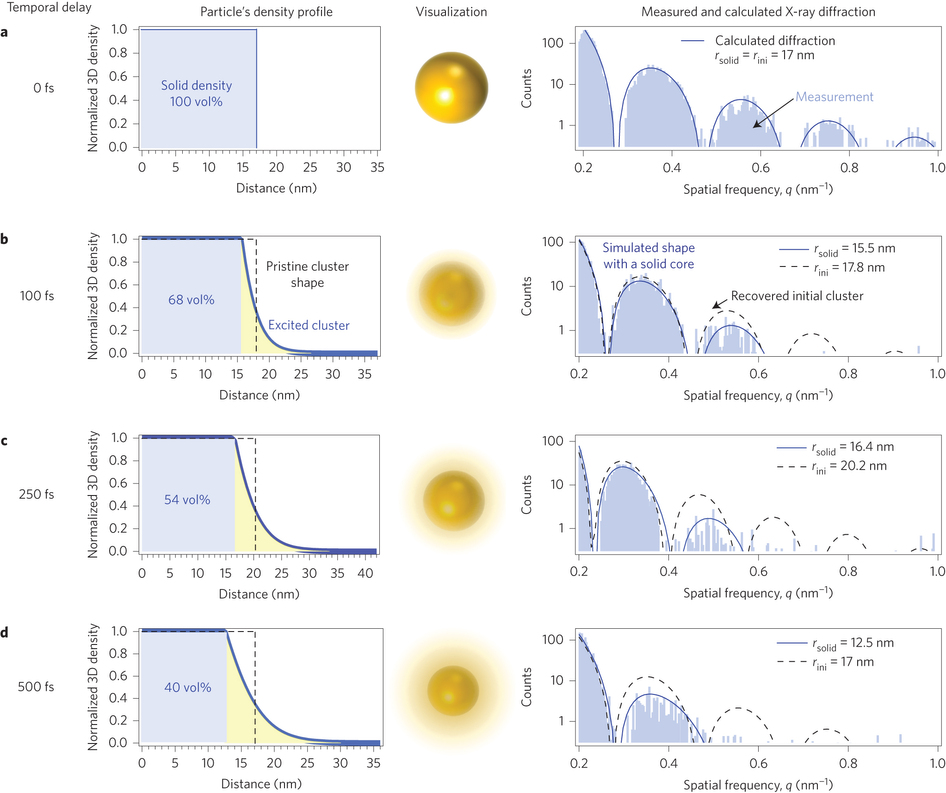
\includegraphics[width=1.00\textwidth]{images/tais-nat-photonics.jpg}
	\caption[Measurement and simulation of the nanoplasma expansion in Xe-cluster.]{Xe-clusters after being pumped with a NIR laser pulse and probed at a certain time delay (indicated left) with a LCLS pulse. Left series, simulation of electron densities. Right series, measured diffraction patterns. The diffraction pattern show a decrease in intensity at larger q values, when the delay is increased. This can be explained through expanding electron densities, i.e., a nanoplasma expansion. Fourier transforms of electron densities are fitted to the measurement for a solid sphere (dashed line) and an expanding sphere (solid line). From \citep{Gorkhover-2016-NatPho}. Reprinted with permission from Nature Publishing Group.}
	\label{fig:tais-nat-photonics}
\end{figure}
%The nanoplasma transition is so interesting is because every matter irradiated by a free-electron laser will undergo a nanoplasma transition and finally disintegrate. This is a challenge for structural biology and called radiation damage  or sample damage \citep{Neutze-2000-Nature}. Sample damage changes the structure of a biomolecule and it is particularly the structure many scientists want to investigate. In order to prevent falsified measurements, one needs to understand the nanoplasma transition as it occurs while the pulse is propagating through the sample.
To study the nanoplasma transition a coincident imaging and spectroscopy technique has proven successful \citep{Bostedt-2012-PRL}. First experiments aimed to revealed correlations between the diffraction patterns and the ion spectroscopic data \citep{Gorkhover-2012-PRL,Rupp-2016-PRL}. The advent of pump--probe techniques has been combined with the coincident measuring technique and recently, snapshots were taken of the expanding electron density \citep{Gorkhover-2016-NatPho}. The snapshots are shown in figure \ref{fig:tais-nat-photonics}. In this particular study, an infra-red laser (pump) was used to cause a nanoplasma transition in a xenon cluster and subsequently image this state with a XFEL pulse (probe). As the time delay between pump and probe pulse is varied, the resulting diffraction patterns of the 15-20 nm Xe-cluster show declining intensities at larger scattering angles with increasing time delay $\Delta t>100 fs$. The loss in signal could be explained through an expanding electron density\index{electron density!expanding} \citep{Hau-Riege-2008-PRE,Peltz-2014-PRL}. The electron density thereby expands increasingly over time due to the Coulomb and Hydrodynamic forces and, first the outer layers expand and at larger time delay also the inner atomic layers. In that study, an electron temperature of ~200eV could be measured by comparing plasma simulations to the ion spectroscopy signal. The spatial resolution of the diffraction patterns has been estimated to be 8 nm but by assuming a spherical shape of the clusters, the electron density model is sensitive below this resolution.\\
\begin{figure}
	\centering
		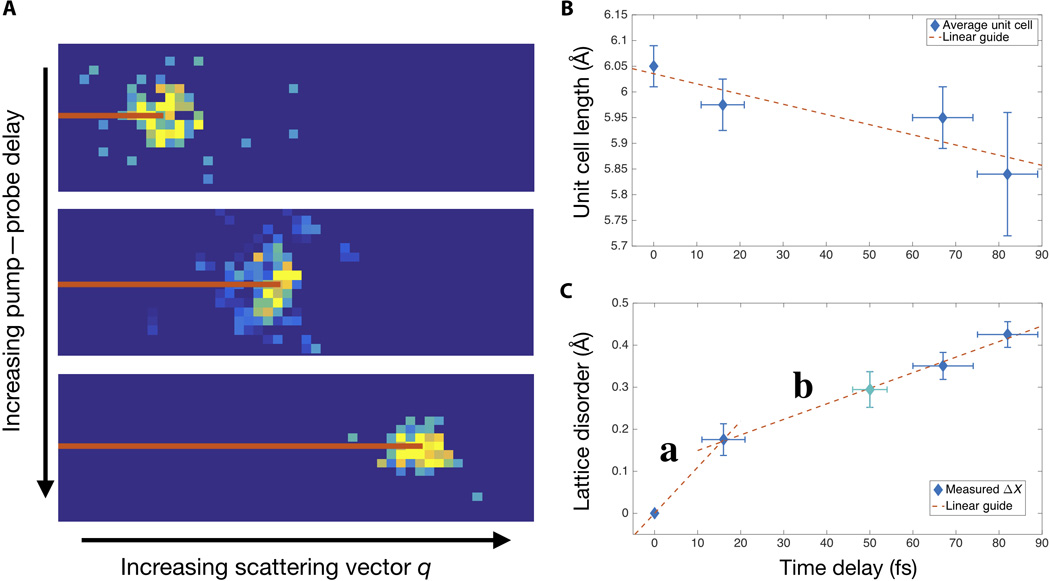
\includegraphics[width=0.80\textwidth]{images/ken-science.jpg}
	\caption[Experiment that shows early evolution of the nanoplasma transition.]{X-ray pump -- X-ray probe scattering experiment on Xe-cluster that shows an early evolution of the nanoplasma transition. A, single-shot Bragg peaks at varying time delays. The scattering vector q increases over time delay. B, unit cell length over time delay. The unit cell length decreases, therefore the cluster shrinks in size. C, Lattice disorder over time delay. The measured fcc lattice is becoming disordered after being pumped with a X-ray pulse. From \citep{Ferguson-2016-SciAdv}. Reprinted with permission from AAAS.}
	\label{fig:ken-science}
\end{figure}
In another study with shorter time delays of $\Delta t<100 fs$, xenon cluster compress in size \citep{Ferguson-2016-SciAdv}. Since clusters form as a crystal\footnote{See section \ref{sec:homogenous-cluster}.}, one can determine their structure through crystallographic approaches as it is explained in full detail in \citep[][chapter 5]{Als-Nielson-2011-JWS}\footnote{In short, crystals scatter light and create Bragg spots at large $\vec{Q}$-values. These Bragg spotts occur when the so called Bragg-law is fulfilled. Bragg's law reads $m \lambda = 2d \sin\left(\frac{\Theta}{2}\right)$,\index{Bragg's law} with $m$ being an integer, $\lambda$ being the wavelength of the scattered light, $d$ the distance between crystalline layers and $\Theta$ the scattering angle. When Bragg's condition is fulfilled, the rays interfere constructively and the location of the Bragg peaks gives insight to the crystalline structure.}. Figure \ref{fig:ken-science}a is showing Bragg peaks under certain conditions over the scattering vector $\vec{Q}$. The signal moves to larger scattering vectors $\vec{Q}$ and, as $\vec{Q}=\frac{2\pi}{a}$, the unit cell length $a$ is shrinking over the time delay $\Delta t = \{0,..,100\}$. This unintuitive and contradictory result is attributed to the changes in electronic configuration upon ionization. Electrons that are trapped in the cluster Coulomb potential have an increased mobility and are able to contribute comparable to valence electrons and therefore change the chemical bonding character of the Van der Waals cluster. As a result, the unit cell changes on the {\AA}ngstrom length scale and the lattice becomes increasingly disordered (see figure \ref{fig:ken-science}c).\\
These two studies allow us to conclude that the nanoplasma transition is a multistep process. First, the initial ionization occurs, followed by an increased Coulomb potential that traps electrons, which then change the structure of the nanosample, e.g. compression of a lattice. Eventually, the system becomes strongly ionized and hot such that Coulomb and hydrodynamic forces start an expansion of the system until the sample disintegrates into its atomic components.
%
%
%
\subsection{Tampered layers to inhibit the nanoplasma expansion}
%%%%%%%%%%%%%%
%- Step by step explanation on the formation of the nanoplasma, pointing out the differences between tampered and pristine clusters
%
%
%%%%%%%%%%%%
%To overcome radiation damage, the most common method is to \textit{outrun} radiation damage\index{radiation damage} processes using very short pulses \citep{Neutze-2000-Nature}.
As we have discussed, the nanoplasma phase-transition occurs on the femtosecond timescale and affects diffraction patterns. To \textit{outrun} this radiation damage, pulses from the XFEL must be shorter than the lifetime of Auger processes, thus few femtoseconds long. And by limiting the XFEL pulse duration, one currently limits the pulse energy\index{pulse energy} as current bunch compression methods typically generate much less fluence. Often, this fluence is not enough and means that many coherent diffractive imaging experiments are currently performed with pulse widths of 40 fs or more to generate enough scattered intensity. But even if these technical limitations can be overcome, outrunning radiation damage does not circumvate photoionization and it is therefore expected that also few femtosecond long pulses only reach a certain spatial resolution \citep{Aquila-2015-StrucDyn}. To be more precise, it is an open question, whether electron densities and here particular bonding configuration are obtainable by solely outrunning radiation damage. As radiation damage is unavoidable it can be mitigated in several ways. One way to mitigate radiation damage would be to simulate the effects, however, this can only be done for small particles. Another way is to fundamentally increase resolution in single particle imaging due to prior alignment of particles such that their orientation is know while the image is taken. Molecule alignment has seen some success for small molecules \citep{Kupper-2014-PRL} but it is currently unknown, whether this works for larger molecules as the strong light fields, which are needed to align the molecules, may change their structure. Here it should be noted that recent advances with CDI algorithms made it possible to computationally determine the orientation of a particle at the time of imaging \citep{Loh-2009-PRE,Ekeberg-2015-PRL} without prior knowledge if at least a few hundred diffraction images are provided. Anyway, in this thesis, we shall discuss a method to reduce effects of radiation damage through artificial tampered layers. Artificial shells around a sample supply it with electrons and function as sacrificial layer that protects the sample \citep{Hau-Riege-2010-PRL}. For aerosol particles, this method has only been investigated through ion spectroscopy \citep{Hoener-2008-JPB,Ziemkewitz-2017-unpublished}.
\begin{figure}
	\centering
		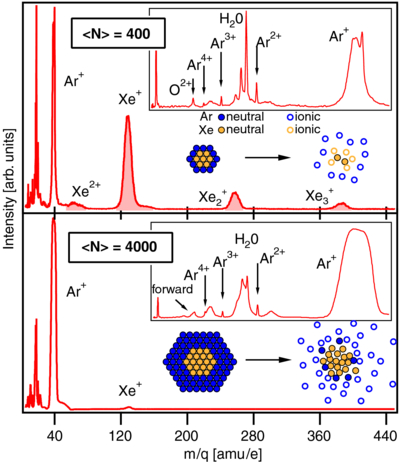
\includegraphics[height=0.50\textwidth]{images/Hoener-image.jpg}
	\caption[Time of flight spectra of argon and xenon core-shell systems.]{Time of flight (TOF) traces of argon and xenon core shell systems irradiated with 93eV X-ray pulses from FLASH\index{Free electron LASer in Hamburg!FLASH}. At this energy, mostly Xe is ionized and the ionized atoms create a steep Coulomb potential that traps electrons towards the center of the cluster. The top panel shows smaller clusters with 400 particles, in which the trapping is inefficient, few electron-ion recombinations occur, thus Xe and Ar ions are detected in the TOF detector. The bottom panel shows large clusters with 4000 particles and a thicker argon shell. Here, Xe-ions recombine in the center and the TOF shows mostly Ar-ions as the neutral xenon remains undetected. From \citep[\href{https://creativecommons.org/licenses/by/3.0/}{\ccby}]{Hoener-2008-JPB}.}
	\label{fig:Hoener-image}
\end{figure}
In the study shown in figure \ref{fig:Hoener-image} a core-shell system of argon and xenon was constructed and here xenon compares to the sample and argon compares to the sacrificial layer around the particle (see figure). The heterogeneous clusters were irradiated with 93 eV photons from \textit{FLASH}\footnote{Short for \textbf{F}ree electron \textbf{LAS}er in \textbf{H}amburg. An extreme ultra violet (XUV) free electron laser in Hamburg, Germany.}\index{Free electron LASer in Hamburg!FLASH}. At this photon energy mostly xenon atoms are ionized. As described in the nanoplasma creation process (see section \ref{sec:nanoplasma-expansion}), the increasing ionized cluster creates a steep Coulomb potential trapping electrons. Trapped electrons are available for recombination with the ionized atoms. In the small core-shell system of ArXe with 400 particles (figure \ref{fig:Hoener-image} top-panel), the time of flight mass spectroscopy\index{time of flight!mass spectroscopy} data show Xe and Ar ions. These ions mean that the charge recombination is suppressed and the cluster disintegrates upon irradiation. In the large ArXe-cluster system with 4000 particles (bottom-panel), mostly Ar ions are in the TOF data. These ions mean that the Xe-ions in the center of the cluster recombine with the electrons that were attracted to the center of the core-shell system due to the steep Coulomb potential of the large cluster. Neutrally charged xenon is not detected by the TOF detector. The Ar-ions in the outer layers contributed electrons to the center of the cluster but were shed off the mixed ArXe-cluster. It is also evident that the argon atoms in the large cluster case release more kinetic energy than in the small cluster case, which is a size-dependent effect that shows an energy transfer process from the initially ionized Xe-core to the Ar-shell.
%
%
%
%
%\newpage
\chapter{Experimental Considerations}\label{ch:exp_setup}
%- Start by introducing LCLS\\
%- Introduction to the AMO instrument at LCLS\\
%- Introduction to the LAMP chamber\\
%- Give example experiments to each point
%\section{The X-ray free electron laser LCLS}
%- Describe LCLS more specifically
%\subsection{LCLS pump probe setup}
%- Specifics to our / LCLSs pump probe setup
The experiment described in the present thesis has been performed using the LAMP end-station of the Atomic, Molecular and Optical (AMO) Physics instrument of the Linac Coherent Light Source, which is located at SLAC National Accelerator Laboratory. SLAC was founded in 1962 as the Stanford Linear Accelerator Center. The linear accelerator was early on used for high-energy physics experiments, which resulted in three Nobel Prizes in Physics \citep{Richter-1976-NP,Taylor-NP-1990,Perl-NP-1995}. SLAC's research topics broadened in the 1970's and with the Stanford Synchrotron Radiation Project, it became an X-ray user facility in 1974. Meanwhile, the synchrotron source was modernized and is now known as the Stanford Synchrotron Radiation Light-source (SSRL) and the linear accelerator was repurposed to function as the world's first hard X-ray free electron laser - the LCLS. The LCLS began operations in April 2009 \citep{Emma-2010-NatPho} and the AMO instrument started user operations in October 2009 \citep{Bostedt-2013-JPB}. AMO began operations with the High-Field Physics (HFP) and the CFEL\footnote{Acronym for the Center for Free Electron Laser Science on the DESY campus in Hamburg, Germany.}-ASG\footnote{Short for the Advanced Study Group of the Max Planck Society in Hamburg, Germany.} Multi Purpuse (CAMP) end-station, which was supplied by the Max-Planck Society from Germany. The so-called ``LAMP'' end-station is a successor of the CAMP end-station and was commissioned in September 2013 \cite{Ferguson-2015-JSR}. LAMP has been in use at the AMO instrument since commissioning and the experiment described in this thesis was performed in January 2014\footnote{Experimental identifier at SLAC: \textsc{amoa1214}} in the LAMP end-station of the AMO instrument. My involvements in design discussions, the building, the commissioning, and the operation of the LAMP end-station were a significant effort during my doctoral studies and resulted - at the time of writing - in the publications \cite{Picon-2016-NatComm,Munke-2016-naturedata,Kimberg-2016-FD,Sanchez-Gonzalez-2015-JphysB,Lehmann-2016-PRA,MacDonald-2016-RSI,Gamboa-2016-JI,Bernado-2017-PRB,Ferguson-2015-JSR}.\\[1\baselineskip]
%
This chapter is organized as follows: Section \ref{sec:amo-instrument} discusses the beam transport from the undulators to the LAMP end-station; Section \ref{sec:LAMP-endstation} focuses on the specifics of the LAMP end-station; Section \ref{sec:pnCCD} goes over the pnCCD X-ray pixel detector and its geometry; Section \ref{sec:sample-delivery} centers around relevant aspects of the sample delivery; Section \ref{sec:TOF-spectrometer} describes the time-of-flight (TOF) spectrometer for the LAMP end-station; and Section \ref{sec:focus-characterization} goes over aspects of the here used X-ray focus characterizations.
%
%
%
%\section[The FEE and AMO instrument at the LCLS]{The front end enclosure and the atomic, molecular and optical physics instrument at the LCLS}\label{sec:amo-instrument}
\section{The X-ray beam transport to the LAMP end-station}\label{sec:amo-instrument}
%%%%%%%%%%%%
%- Specifics to AMO\\
%- For example focus studies and KBOs\\
%- Use JSR and previous AMO articles
%%%%%%%%%%%
The AMO instrument is located closest to the undulators of the LCLS at hutch 1. It is designed for soft X-ray photons in the energy range from \SIrange{280}{2000}{\electronvolt} \citep{Ferguson-2015-JSR,Bozek-2009-EPJST}, where the beam divergence is a limiting factor for lower energies and the boron carbide (B$_{4}$C)-coating on the mirrors leads to absorption above \SI{2000}{\electronvolt} \cite{Bozek-2009-EPJST}. After the X-ray pulse generation in the undulators of the LCLS, the X-rays are separated from the electron bunch using magnets, and optionally, the X-band transverse deflecting structure (XTCAV) \citep{Behrens-2014-NatCom} can be used to give insight into the kinetic energy and pulse duration of the electron bunch. Prior to entering the Front End Enclosure (FEE) \citep{Moeller-2011-NIMPR}, the electron beam is discarded in the electron dump such that only X-rays continue. In the FEE, the X-rays can be attenuated with either gas or solid attenuators. An X-ray pulse energy monitor, often referred to as a gas detector, measures the pulse energy of a single-shot before and after attenuation \citep{Hau-Riege-2010-PRL-2}. Eventually, the X-ray beam is deflected through a mirror system into the desired hutch. To direct the beam to the AMO hutch, the soft X-ray offset mirrors (SOMS) are used. The SOMS are a set of four mirrors, where the first two deflect the X-rays to the LCLS instruments that use soft X-rays, namely the AMO and the Soft X-ray (SXR) instrument \citep{Schlotter-2012-RSI,Soufli-2012-AppOpt,Dakovski-2015-JSR}. The third SOMS mirror is a double mirror that either deflects the beam into the AMO or SXR instrument.
%
\begin{figure}
	\centering
		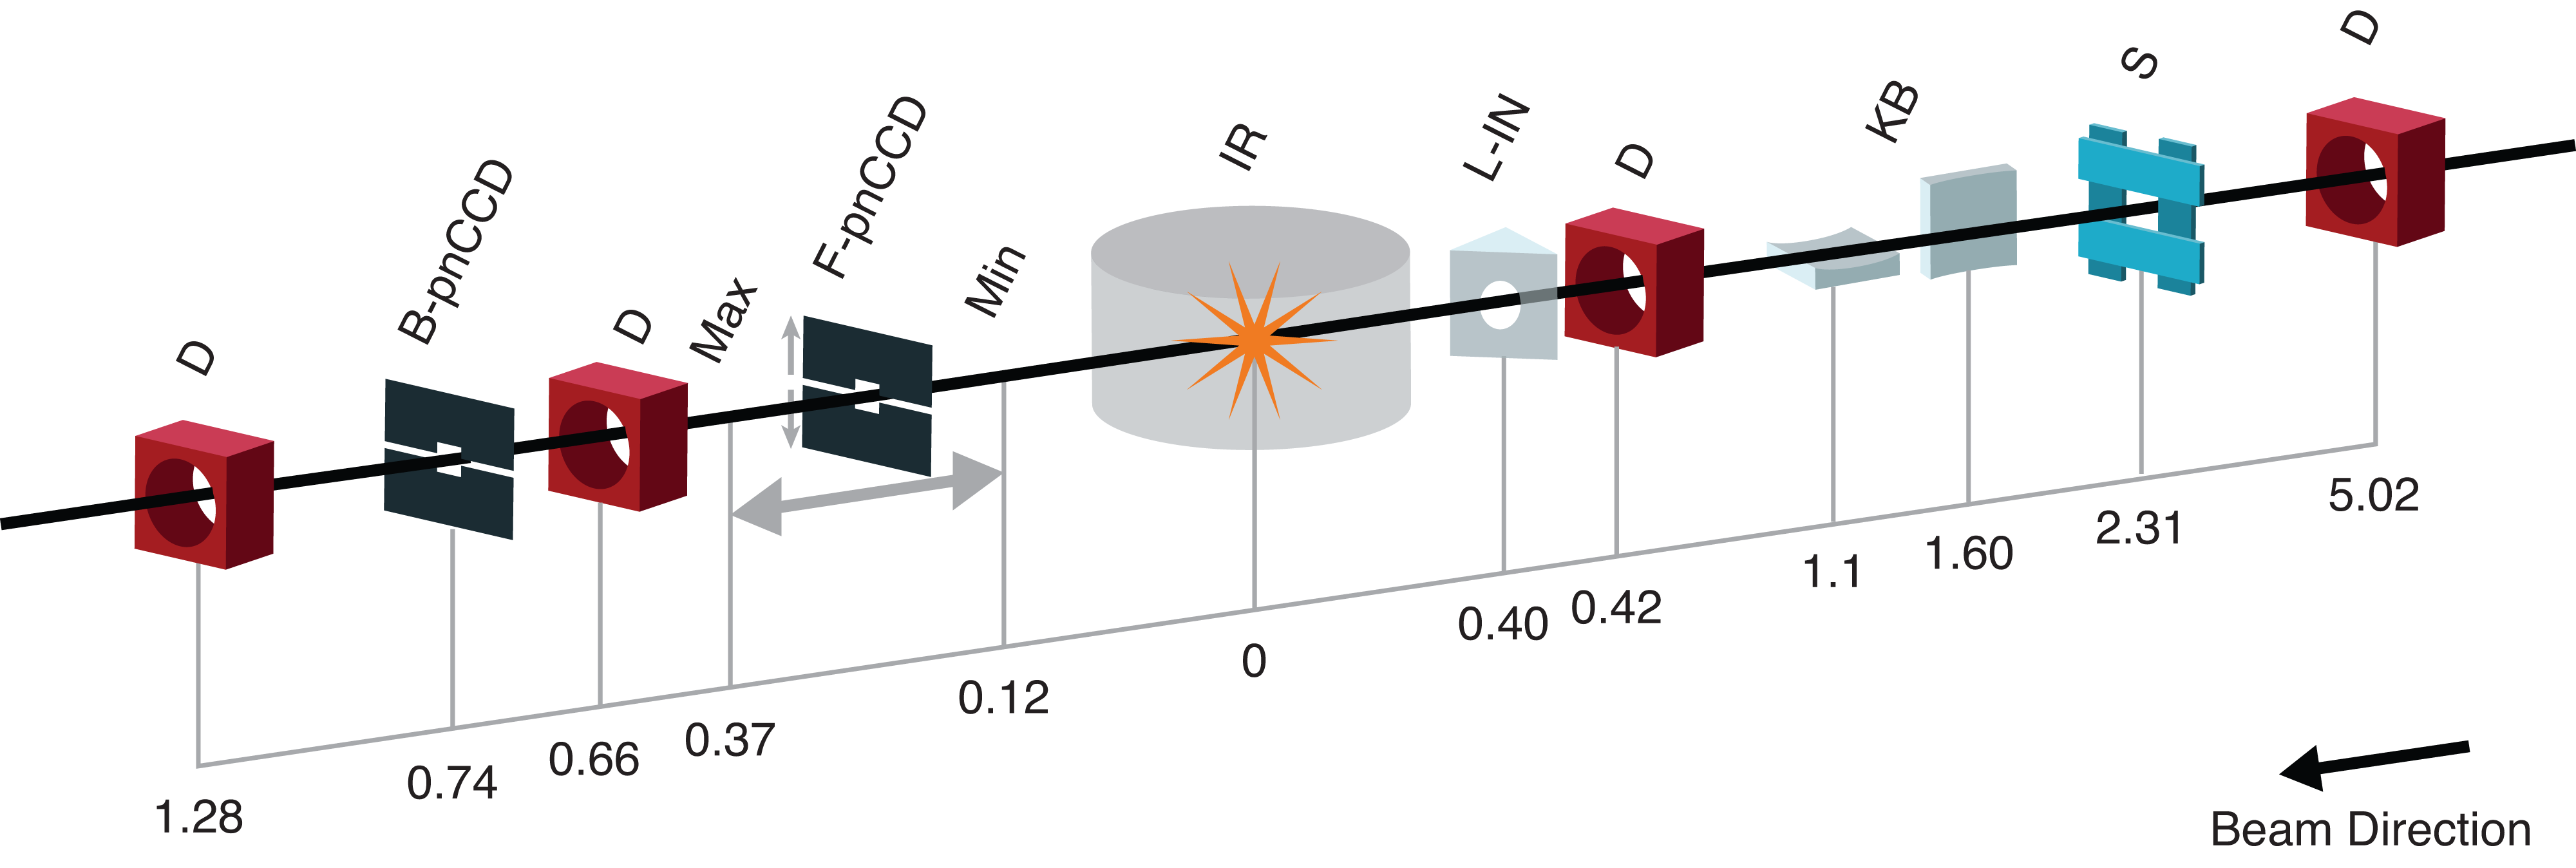
\includegraphics[width=1.00\textwidth]{images/beam_layout.png}
	\caption[Schematic overview of the AMO beamline instrumentation.]{Schematic overview of the AMO beamline instrumentation in the LAMP configuration. The indicated distances below the schematic items are in meters from the interaction region (IR). As the X-ray beam enters the instrument, it can be visualized on a YAG crystal diagnostics (D). A set of 2 slits (S) cuts the beam in the vertical and horizontal to reduce straylight from the Kirkpatrick-Baez (KB) optics. The differential pumping section of the LAMP end-station houses an option to couple-in an optical laser (L-IN). The front and back pnCCD (F/B-pnCCD) are located downstream of the IR. From \citep{Ferguson-2015-JSR}.}
	\label{fig:beam_layout}
\end{figure}
%
The AMO instrument is versatile in its configuration and four different end-stations have been used so far. In historic order: one, the HFP end-station \citep{Bozek-2009-EPJST,Bostedt-2013-JPB}; two, the diagnostics (DIA) end-station \citep{Bostedt-2013-JPB}; three, CAMP end-station \citep{Strueder-2010-NIMPA}; and four, the LAMP end-station \citep{Ferguson-2015-JSR,Bucher-2016-Unpublished}. Today, the HFP and LAMP end-station can be combined with additional instrumentation, for example, the modernized DIA end-station or the XRSD device (see Section \ref{sec:novel-pump--probe-tech}). As the experiment described in the present work has been performed with the LAMP end-station, we shall focus on that AMO configuration from here on.\\[1\baselineskip]
%
A schematic overview of the AMO beamline instrumentation in the LAMP configuration can be found in Figure \ref{fig:beam_layout}. As the X-ray beam travels from the FEE to the AMO beamline, it can be viewed with a YAG crystal diagnostic viewer (D). Here the shape and position of the beam can be determined as it is several meters downstream of the SOMS such that a difference of the SOMS angle and position can be determined with sub-millimeter precision. This also reveals the alignment of the beam with respect to several differential pumping apertures that are located in the FEE. Experience shows that the X-rays should be centered to those apertures \citep{Turner-2016-PC}. This diagnostic viewer is also useful to detect and correct for an unstable X-ray beam or erratic beam pointing.
%It is noteworthy already here in the text that the X-ray beam became unstable and the beam's pointing became erratic. The most upstream diagnostic viewer (D) of the AMO instrument was able to detect this jitter such that the linear accelerator could be tuned to correct the erratic pointing. 
A beamline alignment laser, which is a typical HeNe-laser with low beam divergence, can be coupled into the beamline slightly downstream of the YAG screen\footnote{Not shown in  Figure \ref{fig:beam_layout}} such that it co-propagates with the X-rays. 
%Beamline alignment lasers are invaluable tools to pre-align a system before X-rays are employed. For the described experiment, it was necessary to align the particle jet of the pristine Xe-cluster and the particle jet of the HeXe-cluster to be perpendicular to the X-ray beam (see Figure \ref{fig:Overview-Jetalignment}). 
%In order to perform this alignment, a beamline alignment laser that co-propagates with the X-rays was useful, if not required. 
The X-ray beam then travels through a set of four blades (S), which are often referred to as 4 Jaw slits that can be moved independently to cut into the beam and reduce parasitic scattering\footnote{Parasitic scattering is often referred to as stray light.} originating from the Kirkpatrick-Baez (KB-)mirrors \citep{Kirkpatrick-1948-JOSA}.
%In collaboration with the Single-Particle Initiative \citep{Aquila-2015-StrucDyn}, it was investigated how the blades reduce unwanted scattering. It was found   \citep{SPI-2015-unpublished}
Experience shows that the blades should not cut into the main intensity profile of the beam but rather conservatively cut into the halo of the beam. This sufficiently reduces parasitic scattering but does not significantly reduce the peak intensity of the X-ray pulse (compare green and blue curve in Figure \ref{fig:Focus-z-scan}).\\[1\baselineskip]
%
The KB-mirrors are a set of two concave mirrors that focus the X-ray beam into the interaction region \cite{Bostedt-2013-JPB}. The mirrors consist of two \SI{400}{\milli\meter} long silicon (Si) substrates that are coated with boron carbide. They reflect the X-rays in grazing incidence at \SI{13.85}{\milli\radian} and are sometimes referred to as KB-optics. The first mirror focuses the beam in the horizontal and the second mirror focuses the beam in the vertical. As the mirrors are located at different positions in the horizontal and vertical, they are designed to have a focal length of \SI{1600}{\milli\meter} in the horizontal and \SI{1100}{\milli\meter} in the vertical. Additionally, the mirrors can be bent to change their focusing position along the $Z$-axis\footnote{The LCLS uses a right-handed coordinate system, where the index finger ($Y$-axis) points up and the middle finger ($Z$-axis) points colinear to the X-ray beam.} and the optimal focus can be found and characterized by, for example, studying time-of-flight \index{time-of-flight} spectra \citep{Bucher-2016-Unpublished} and analyzing imprints\index{imprint} \citep{Hajkova-2011-SPIE,Chalupsky-2011-NIMPR}, which we will discuss in Section \ref{sec:focus-characterization}. A study of the X-ray focus is necessary to achieve the smallest focus, thereby increasing the intensities at the sample interaction region.
% which is desired in coherent diffractive imaging as thus more photons scatter from the sample and, ideally, to understand the coherent wavefront that creates an image of the particle better.
%
%
%
%
For the experiment in this thesis, the X-ray beam focal size was determined to be $\text{FWHM}\approx \SI{1.5}{\micro\meter}$, with an effective area of $\SI{5}{\micro\meter\squared}$ \citep{Bucher-2016-Unpublished}. The LCLS beam parameters are summarized in Table \ref{tab:beam-params}. The pulse duration was determined through analysis of the electron beam and the delay, $\Delta$t, precision is estimated from geometric considerations of the delay chicane (see Section \ref{sec:novel-pump--probe-tech}).
\begin{table}
	\centering
		\begin{tabular}{ | l | l | l | }
		\hline
			 & pump beam & probe beam  \\ \hline
			wavelength & \multicolumn{2}{|c|}{\SI{1.5}{\nano\meter}} \\ \hline
			mean pulse energy & \SIrange{80}{100}{\micro\joule} & \SIrange{0.8}{1}{\milli\joule} \\ \hline
			X-ray beam FWHM & \multicolumn{2}{|c|}{\SI{\sim 1.5}{\micro\meter}} \\ \hline
			pulse duration & \multicolumn{2}{|c|}{\SI{\sim 25}{\femto\second}} \\ \hline
			delay $\Delta$t precision & \multicolumn{2}{|c|}{\SI{<1}{\femto\second}} \\ \hline
		\end{tabular}
	\caption{Summary of LCLS beam parameters during experiment.}
	\label{tab:beam-params}
\end{table}
%
%
%
\section{The LAMP end-station at the AMO instrument}\label{sec:LAMP-endstation}
%%%%%%%%%%%%%%%%%%
%- Specifics to the LAMP setup\\
%- Use Journal of Synch. Radiation LAMP paper\\
%- I think this can be a longer subsection since a lot of my work went into this.
%%%%%%%%%%%%%%%%%%%
\begin{figure}
	\centering
		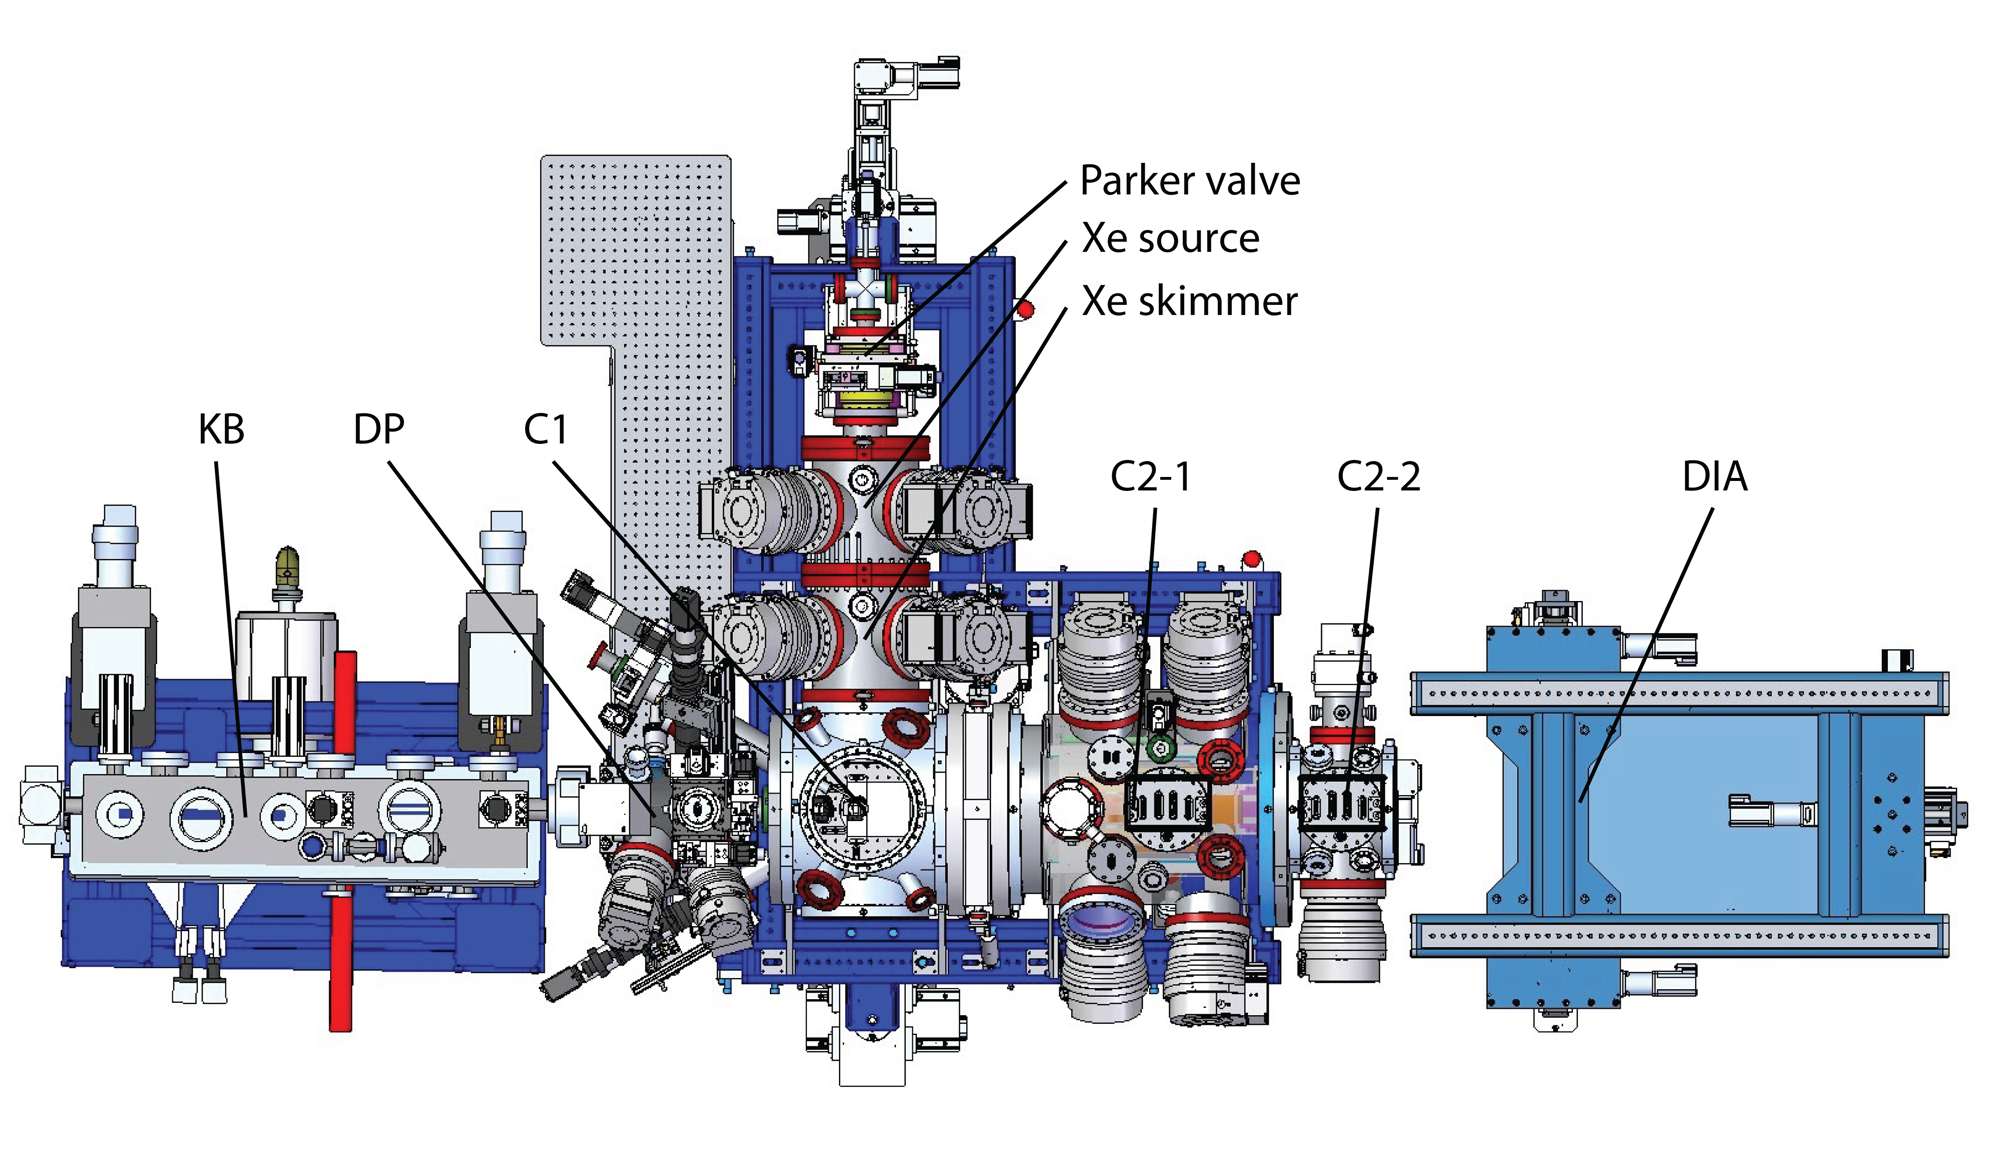
\includegraphics[width=0.75\textwidth]{images/AMO-overview-4.png}
	\caption[Overview of the AMO instrument in the LAMP end-station configuration.]{Overview of the AMO instrument in the LAMP end-station standard configuration. From left to right, the beam propagates through the Kirkpatrick-Baez (KB) optics, the differential pumping (DP) section, the interaction chamber (C1), the front pnCCD chamber (C2-1), the rear pnCCD chamber (C2-2) and finally the diagnostics (DIA) stand. The Xe jet is also shown, including the Parker valve, Xe-source and -skimmer chamber, which are mounted on C1.
%The xenon jet is installed including the manipulator that holds the Parker valve, the Xe source chamber and the Xe skimmmer chamber. The helium jet is not included in this drawing but mounted perpendicular to the Xe jet and the vacuum pumps have not been installed as shown here. For scale, the large, open conflat flanges on the C1 chamber are 12 inch.
}
	\label{fig:LAMP-overview}
\end{figure}
%
After the KB-mirrors, the X-ray beam enters the LAMP end-station, which is indicated in the beamline schematic of the AMO instrument in Figure \ref{fig:beam_layout} and the overview of the AMO instrument in Figure \ref{fig:LAMP-overview}. LAMP begins with a differential pumping (DP) section that separates the interaction (C1) and detector chambers (C2-1, C2-2) from the KB optics and other upstream beamline instrumentation. The differential pumping section consists of two small tubes, which are pumped with turbo-molecular pumps at neighboring chambers. The tubes are \SI{5}{\milli\meter}, \SI{8}{\milli\meter}, or \SI{10}{\milli\meter} diameter differential pumping apertures that are indicated in Figure \ref{fig:c1-ccd-spec} and are exchangeable. The DP stage is able to maintain over 4 orders of magnitude pressure difference, for example, the pressure in the C1 vacuum chamber, $p_{\text{C1}}$, may rise to $p_{\text{C1}}=\SI{e-6}{\kilo\pascal}$ due to the sample injection, but the pressure in the KB-optics vacuum tank, $p_{\text{KB}}$, is maintained at $p_{\text{KB}}=\SI{e-10}{\kilo\pascal}$ due to the differential pumping section. The second DP-stage chamber holds a YAG crystal to examine the X-ray beam after the KB optics and a removable laser in-coupling mirror to overlap X-rays with an optical laser or an aperture to reduce parasitic scattering from the differential pumping apertures and upstream elements.\\[1\baselineskip]
\begin{figure}
	\centering
		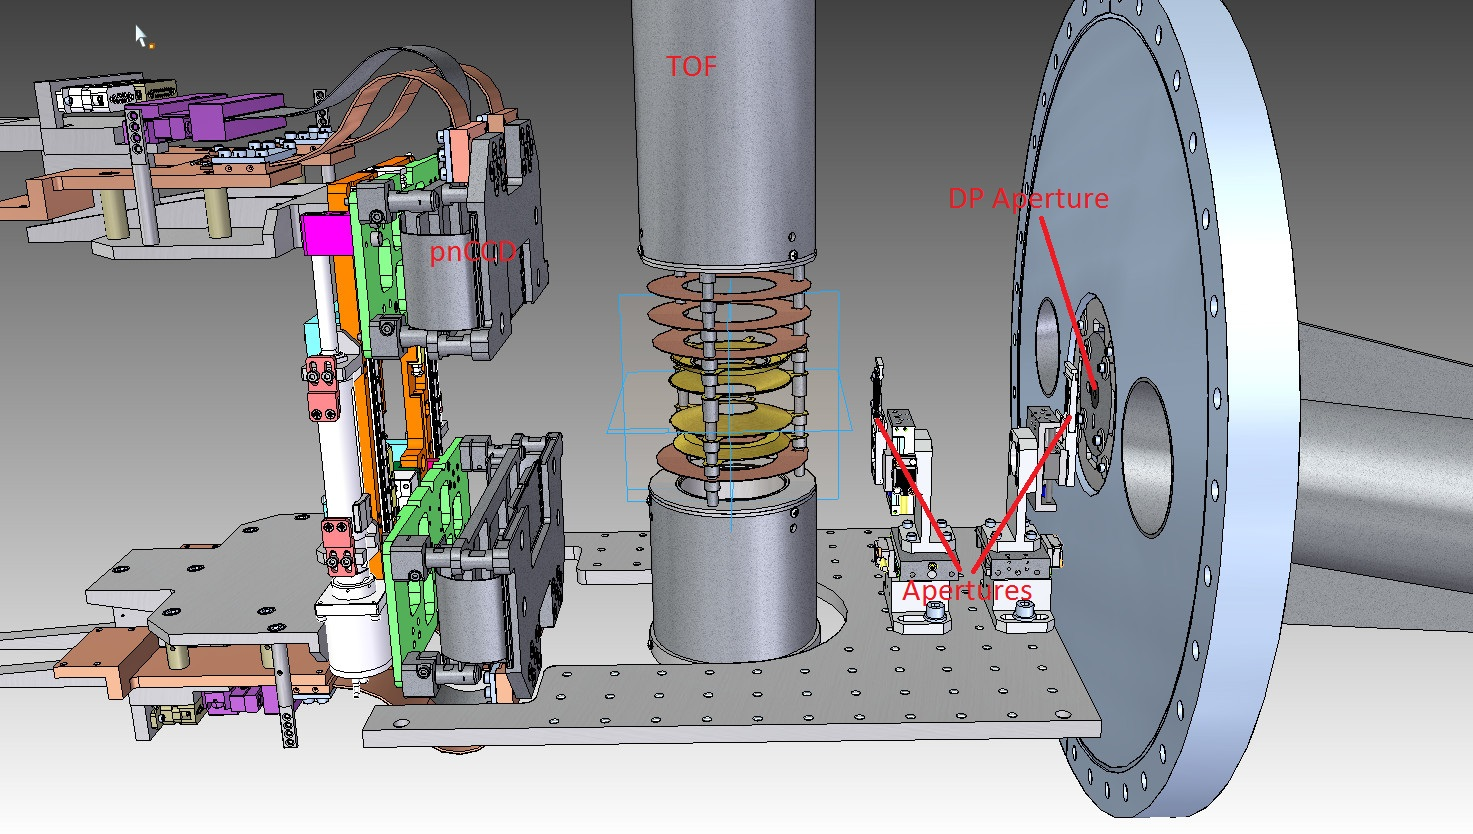
\includegraphics[width=1.00\textwidth]{images/c1-ccd-spec.jpg}
	\caption{Inside view of the C1 chamber showcasing the interaction region.}
	\label{fig:c1-ccd-spec}
\end{figure}
%
The beam then travels into the C1 chamber that encloses the interaction region. Before reaching the sample interaction region, the beam is cut by apertures (see Figure \ref{fig:c1-ccd-spec}). The apertures are mounted on encoded stages that are driven by piezoelectric actuators with sub-micron movement precision. Experience shows that a useful aperture material for the AMO instrument beam parameters is silicon nitride ($\text{Si}_{3}\text{N}_{4}$). These silicon nitride substrates have windows with tapered-edges, which can be used to cut into the X-ray beam without generating significant scattering of the tapered edges. The window-size can be fit to the size of the X-ray beam diameter, which can be estimated using geometric optics. Alternatively, oversized aperture windows can be used to drive one corner of the window on the first aperture stage and the opposite corner on the second stage into the beam, which is sometimes referred to as cornering apertures. As part of this thesis work, an improved aperture system was designed using four aperture blades with tapered edges. These allow full control over the aperture from four directions, thus allowing short aperture alignment times and a more controlled reduction of unwanted effects. For soft X-rays, it is important to note that the flat side of the tapered aperture is facing the beam such that the tapered-edges are facing downstream.\\[1\baselineskip]
%Otherwise unwanted reflections may occur. This aperture system was commissioned in 2015 for diffractive imaging experiments at the AMO instrument.
\begin{figure}
	\centering
		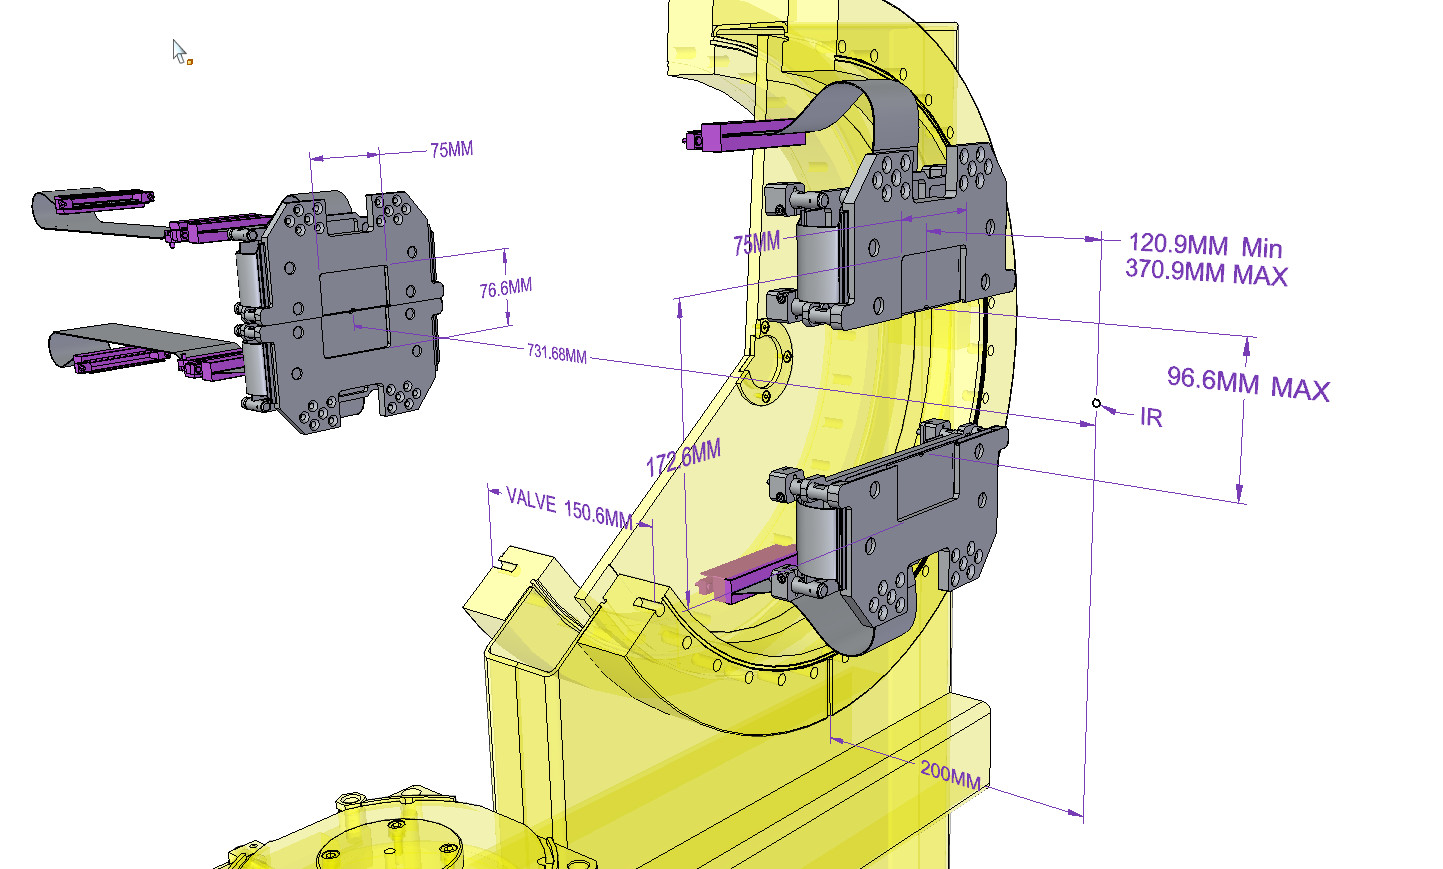
\includegraphics[width=1.0\textwidth]{images/pnCCD-dimensions.jpg}
	\caption[pnCCD detector geometry in the LAMP instrument.]{View of the pnCCD detector geometry inside LAMP. The interaction region (IR) is in the center of C1. The beam propagates along the $Z$-axis, where the rear (top) pnCCD is placed \SI{728.53}{\milli\meter} away from the interaction region (original engineering distances). The half detector height is \SI{38.3}{\milli\meter} and results in a scattering angle of $\Theta =$ \SI{4.3}{\degree}. With the gate-valve installed, the front pnCCDs are able to travel along the $Z$-axis from \SIrange{121}{371}{\milli\meter} downstream of the interaction region. The front pnCCDs can be moved along the $Y$-axis and at maximum extension, the outer corners of the front pnCCD detector correspond to a scattering angle of $\Theta=$ \SI{38.1}{\degree}.}
	\label{fig:pnCCD-dimensions}
\end{figure}
%
In the center of C1, where sample and X-rays interact, a time-of-flight spectrometer can be installed (see Figure \ref{fig:c1-ccd-spec}), which is described in detail in Section \ref{sec:TOF-spectrometer}. The beam then enters the C2-1 chamber through a large gate valve. Here, a variety of distances become relevant for the digital combination of diffraction images from the front and rear pnCCD detectors (see Section \ref{sec:pnCCD}). The algorithm to combine the images is discussed in detail in Section \ref{sec:combination-of-images}, but the following discusses the design distances. Figure \ref{fig:pnCCD-dimensions} shows the pnCCD detector geometry inside the LAMP instrument including the gate-valve. The manufacturing size of the gate-valve along the $Z$-axis is \SI{150.6}{\milli\meter}. The front pnCCD is mounted on a motorized stage and can be moved along the $Z$- and $Y$-axis inside the vacuum. The front-bottom pnCCD module can be set between \SIrange{117.75}{367.75}{\milli\meter} downstream of the center of C1 along the $Z$-axis. The front-top pnCCD module is mounted fix with respect to the bottom module and is always \SI{3.15}{\milli\meter} closer to C1. The maximum extent along the $Y$-axis is \SI{48.3}{\milli\meter} from the beam to the onset of the detector. In the thesis experiment, the front pnCCD modules were in the most rear position and their extent along the $Y$-axis was asymmetric, whereby the front-top pnCCD was \SI{17.3}{\milli\meter} from the beam and the front-bottom pnCCD was \SI{18.9}{\milli\meter}. The distance from the center of C1 to the bottom-rear pnCCD detector module is \SI{731.68}{\milli\meter} and the top-rear pnCCD module is again \SI{3.15}{\milli\meter} closer to C1\footnote{These design distances must be extended by \SI{\sim + 5}{\milli\meter} along the $Z$-axis due to customization during the initial setup of LAMP.}. A set of motorized, in-vacuum stages allow the use of another YAG crystal (D), an optical filter and a B$_{4}$C beam stop just before the rear pnCCD. In this thesis, both pnCCD detectors were used such that another B$_{4}$C beam stop and Yag crystal was mounted on a motorized stage behind the rear pnCCDs to stop the X-rays.
%
%
%
\section{The large area pnCCD detectors}\label{sec:pnCCD}
%%%%%%%%%%%%%%%%%%%%
%- Reuse our work on the LAMP-pnCCD paper\\
%- I think this should be a longer chapter since a lot of my work has gone into this.
%%%%%%%%%%%%%%%%%%%%
The pnCCDs are attractive photon area detectors for the following four reasons \cite{Hartmann-2006-NIMA,Ordavo-2011-NIMA}: one, their high quantum efficiency (QE) and good signal to noise ratio; two, their read-out rate is very high -- up to $\SI{200}{\hertz}$; three, their large active areas cover wide scattering angles; and four, the detectors are almost defect free after applying widely-used pixel detector image corrections. pnCCDs were originally designed to be sent into space and have found usage in astronomy and material science \cite{Struder-2001-AA}. The pnCCD detectors have been used first as X-ray diffractive imaging detectors at FLASH and at LCLS, namely in the CAMP instrument \cite{Strueder-2010-NIMPA}. At LCLS, these detectors are mostly used for X-ray diffractive imaging, but they also have spectroscopic capabilities, which are demonstrated in the left panel of Figure \ref{fig:pnCCD-histogram}. For this thesis, the pnCCD detectors were used to record diffraction images and are described in detail below.\\[1\baselineskip]
%
\begin{figure}
	\centering
   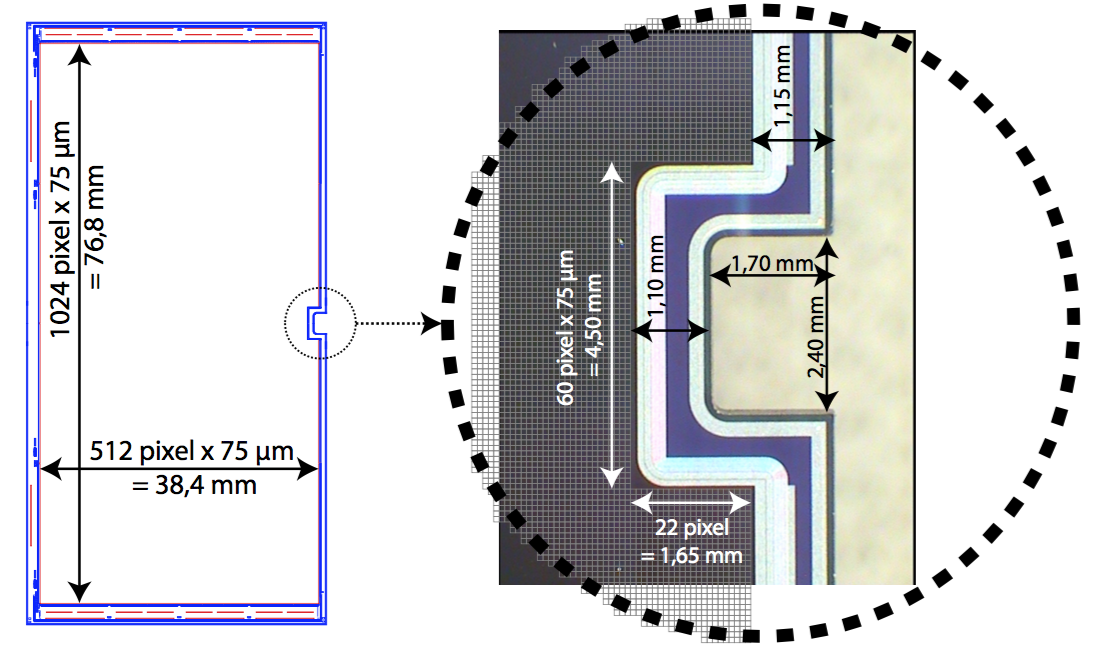
\includegraphics[width=0.7\linewidth]{images/pnCCD-detail.png}
    \caption[Geometry of a single pnCCD module.]{Geometry of a single pnCCD module with a detailed view of the beam conveying hole. A single module consists of \SI{1024 x 512}{\pixels}. Each pixel is $\SI{75 x 75}{\micro\meter}$, which results in an active area of \SI{76.8 x 38.4}{\milli\meter}. The chip is surrounded by non-active edges, which are \SI{1.15}{\milli\meter} wide on beam facing edges. The hole reduces the active area on one module by \SI{60 x 22}{\pixels}, or \SI{4.5 x 1.65}{\milli\meter} and allows the beam to propagate through a \SI{2.4 x 1.7}{\milli\meter} hole.}
\label{fig:ccd-detail}
\end{figure}
%
Let us begin by describing the chip geometry \citep{Bucher-2016-Unpublished}. Each front or rear pnCCD detector is made out of two modules. Figure \ref{fig:ccd-detail} shows the layout of a single pnCCD module\index{pnCCD!module}. The chip consists of \SI{512 x 1024}{\pixels}. Each pixel has a size\index{pnCCD!pixel size} of \SI{75 x 75}{\micro\meter}, so the area that the detector covers is \SI{38.4 x 76.8}{\milli\meter}. To allow the FEL beam to travel through the instrument, each module has a rectangular region cut out in the middle of the center edge. On a single module this area is \SI{4.5 x 1.65}{\milli\meter} and for the whole detector this ``hole'' has the dimensions \SI{4.5 x \sim 4.5}{\milli\meter}. The rear pnCCD position has been chosen such that the pnCCD hole slightly oversizes the diverging FEL beam, when the focus is in the middle of the C1 chamber. The borders of each module are insensitive to photons over a width of \SI{1.15}{\milli\meter} and \SI{1.10}{\milli\meter} at the borders of the hole. To minimize the overall detector area that is insensitive to photons, the two pnCCD\index{pnCCD} modules are mounted such that the non-sensitive areas overlap. As a result of that, each top module is \SI{3.15}{\milli\meter} closer to the interaction region than the corresponding bottom module. The effective gap that is seen in the laboratory frame images between each top and bottom module measures \SI{16}{\pixels} or \SI{\sim 1.2}{\milli\meter}.\\[1\baselineskip]
%
The pnCCD chip is read out with a custom CMOS multichannel Analog MultiplEXer (CAMEX)\index{pnCCD!CAMEX}. Eight CAMEX are installed on each pnCCD module, which are indicated on top and bottom of the pnCCD module overview in Figure \ref{fig:ccd-detail}. The CAMEX performs two interesting functions; one, instead of reading out every pixel sequentially, it can read-out $128$ pixel rows in parallel enabling pnCCD image read-out rates of up to \SI{200}{\hertz}; two, it pre-amplifies the photon signal through a set of gain amplifiers. For this thesis experiment, the pnCCD gain settings become interesting as they need to be considered when combining detector images and are discussed in detail below.\\[1\baselineskip]
% and three, it converts the signal to an analog output. The analog output containing the image information is converted to a digital signal and stored by the LCLS Data Acquisition (DAQ)\index{pnCCD!Data Acquisition} in the LCLS psana\index{psana} network, where it is accessible for analysis (see Section \ref{sec:LCLS-computing}).\\[1\baselineskip]
\begin{table}%[h!]
\centering
\begin{tabular}{ |c c c c |}
 \hline
 Key & relative  & approx.  & max. photons \\ 
     &   gain    & ADU/keV  & per pixel  \\
 %a & b & c & d & e \\
 %[0.5ex] 
 \hline
 1 & $1/256$ & 5 & 1100  \\
 2 & $1/128$ & 10 & 640   \\
 3 & $1/64$ & 20 & 320   \\
 4 & $1/16$ & 79 & 80  \\
 5 & $1/4$ & 316 & 20  \\
 6 & $1$ & 1250 & 5  \\
 \hline
\end{tabular}
\caption[pnCCD gain modes and typical ADU values at \SI{1}{\kilo\electronvolt} photons.]{Typical generated ADU values and dynamic range using \SI{1}{\kilo\electronvolt} photons at all pnCCD gain settings. It is a valid approximation to linearly extrapolate to other photon energies.}
\label{tab:gain-modes}
\end{table}
%
Different gain modes\index{pnCCD!gain} can be used to be more sensitive to photons at high gain or to store signal from more photons at low gain. Table \ref{tab:gain-modes} shows information about the pnCCD gain settings and arbitrary detector units (ADU) generation.
%The different gain amplifications are applied through the CAMEX.
Gain $\tfrac{1}{1}$ is the highest gain and $\tfrac{1}{256}$ is the lowest gain. As one steps from highest to lower gains, e.g., from $\tfrac{1}{1}$ to $\tfrac{1}{64}$, the ADU value creation per photon goes with that fraction in good approximation.\\[1\baselineskip]
%Hence, going to lower gains reduces the signal-to-noise ratio but more photon signal can be stored.
%Note, that the table shows typical operating values using $1$ keV photons and that the ADU value creation is dispersive.
%
Another useful consideration for an experiment using the pnCCD detectors is the quantum efficiency and gain behavior of the pnCCD chip at various wavelengths. The pnCCD is ``back illuminated'' and the entrance windows are coated with a thin aluminum layer to reduce their sensitivity to optical light. For the soft X-ray operating range at the AMO instrument of \SIrange{280}{2000}{\electronvolt}, this aluminum coating attenuates the X-rays only slightly and the detectors maintain a quantum efficiency of \SI{\sim 90}{\percent} \cite{Strueder-2010-NIMPA}. At the AMO instrument, it is thus possible to linearly estimate the generated ADU values from elastic scattering at various photon energies, for example, a \SI{1}{\kilo\electronvolt} photon will generate approximately \num{1250} ADU in highest gain (compare Table \ref{tab:gain-modes}) and a \SI{1.5}{\kilo\electronvolt} photon will generate approximately \num{1750} ADU in highest gain (compare Figure \ref{fig:pnCCD-histogram}). For the photon energy of \SI{837}{\electronvolt} used in this thesis experiment, photons approximately generate \num{\sim 1087} ADU in highest gain. The highest gain has been applied to the front pnCCD detector and the rear pnCCD detector was set to gain $\tfrac{1}{64}$. For the gain $\tfrac{1}{64}$, the ADU value generation per \SI{837}{\electronvolt} photon can be estimated as $\tfrac{1087}{64}$ ADU $\approx 17$ ADU.
%For completeness, it should be noted that the pnCCDs can be optionally mounted with an Al-filter in front of the entrance windows to reduce effects of optical or infra-red laser light, which were not mounted in this experiment. However, there is an Al-filter mounted on the opposite side of the entrance windows that attenuates scattering from the rear of the chamber and beam stop or so-called ``back scattering''.
%
%
%TBD The thin and unstructured radiation entrance windows have a high quantum-efficiency from the infra-red (IR) to soft X-ray wavelength range. In order to avoid unwanted scattering, the photon entrance windows are located at the back of the detector, thus facing upstream of LCLS, and are coated with \SI{50}{\nano\meter} aluminum to reduce their sensitivity to optical light. This aluminum coating does attenuate the soft X-rays at AMO slightly but the detectors maintain a quantum efficiency of \SI{\sim 90}{\percent}. At AMO, it is thus possible to linearly extrapolate the generated ADU values to other photon energies, for example, a \SI{1.5}{\kilo\electronvolt} photon will generate approximately \num{1750} ADU in highest gain (compare Figure \ref{fig:pnCCD-histogram}). The in this thesis used \SI{837}{\electronvolt} photons will approximately generate \SI{\sim 1087}{\electronvolt}. There is also an optical aluminum filter mounted from the front of the chip, thus facing downstream of LCLS, to drastically reduce wrongly directed scattering.
%
%
%
\section{Sample delivery}\label{sec:sample-delivery}
%\subsection{Xe - cluster}
%- I can probably recycle the usual here
%\subsection{He - cluster}
%- Experimental setup\\
%- Info from Andrey probably needed
%\subsection{HeXe - cluster}
%- Experimental setup\\
%- Info from Andrey probably needed
\begin{figure}
	\centering
		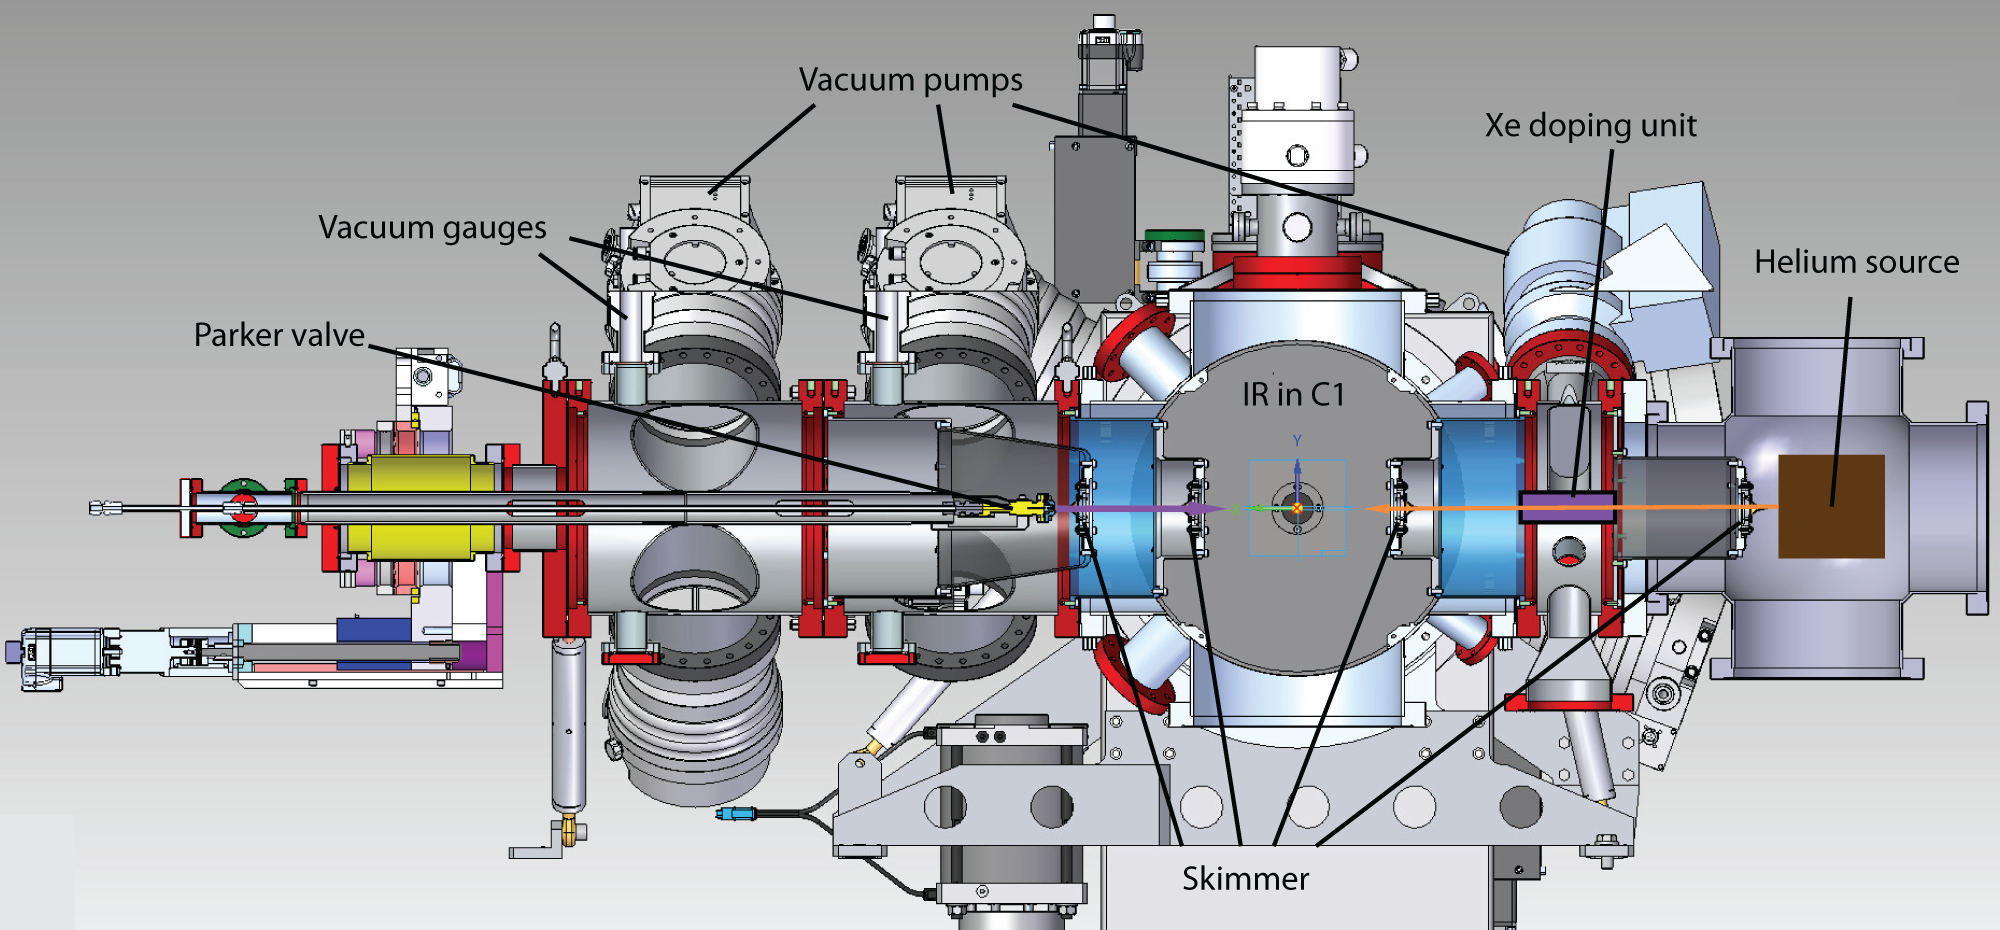
\includegraphics[width=1.00\textwidth]{images/amoa1214-querschnitt.png}
	\caption[Sideview of double sample jet configuration.]{Downward view of a slice through the interaction region in C1 of the experimental setup. The purple arrow indicates the xenon gas flow, the orange arrow indicates the helium gas flow.}
	\label{fig:Overview-Jetalignment}
\end{figure}
For this experiment, two gas sources are used in order to create single rare-gas clusters: one, a pulsed gas source for high pressure xenon operations at room temperature; and two, a continious gas expansion source for helium operations that is cryogenically cooled. Given the time constraint of performing experiments at the LCLS, both sources are installed in one setup and operate independently, allowing quick sample changes. A schematic setup of the sample environment can be found in Figure \ref{fig:Overview-Jetalignment} and a list of used vacuum pumps can be found in Table \ref{tab:vacuum-table}. The principle of the cluster generation is discussed in Section \ref{sec:homogenous-cluster} and \ref{sec:heterogeneous-cluster}. Experimental aspects of the gas sources and operations is discussed in the following.\\[1\baselineskip]
%Single xenon and helium clusters are produced using the principle of the supersonic gas expansion into a vacuum that is described in Section \ref{sec:homogenous-cluster}. Helium clusters that are doped with xenon are produced through the pickup principle as described in Section \ref{sec:heterogeneous-cluster}. Given the time constraint of performing experiments at the LCLS, both sources are installed in one setup and operate independently, allowing quick sample changes. A schematic setup of the sample environment can be found in Figure \ref{fig:Overview-Jetalignment} and a list of used vacuum pumps can be found in Table \ref{tab:vacuum-table}.\\[1\baselineskip]
\begin{table}
	\centering
\begin{tabular}{ | l | l | l | }
\hline
	\textbf{Chamber} & \textbf{Turbomolecular pump mod.} & \textbf{Roughing pump mod.} \\ \hline
	Xenon source & 4x Leybold Turbovac TMP 361 & \multirow{4}{*}{adixen ACG600} \\ 
	Xenon skimmer & 2x Leybold Turbovac Mag W 300 P &  \\ 
	Helium source & 2x Leybold PK-S 1300 & \\ 
	Helium skimmer & 2x Pfeiffer HiPace 300 & \\ \hline
	LAMP C1 & 1x Pfeiffer HiPace 700 & \multirow{2}{*}{adixen ACP 120G} \\ 
	LAMP C2-1 & 4x Pfeiffer TC 400 & \\ \hline
\end{tabular}
\caption[Installed vacuum pumps in the experiment.]{Installed vacuum pumps per chamber in the experiment.}
\label{tab:vacuum-table}
\end{table}
The AMO cluster source, which produces xenon clusters, consists of a Parker-Hannifin Series 99\footnote{Series 99 is at the time of writing not produced/advertised as a straight, in-line pulsed valve anymore.} pulsed valve using a solenoid with a custom manufactured conical copper nozzle, two vacuum chambers to mount two skimmers, a slit that is adjustable through a piezoelectric motor, and several vacuum pumps. It is a well-characterized source that was used extensively in the past \citep{Ferguson-2016-SciAdv,Ferguson-2015-JSR,Gorkhover-2012-PRL,Gorkhover-2016-NatPho,Rupp-2014-JCP}. The pulsed solenoid valve (see Figure \ref{fig:parker-valve}) is controlled with a Parker-Hannifin Iota One pulsed-valve driver. The valve driver applies a current to the solenoid, a magnetic cylinder with the attached poppet actuates and opens the valve. After the TTL signal from the driver ends, the valve closes again. The valve's opening time is set to 1 ms and repetition rates of up to $30$ Hz can be set at a xenon reservoir pressure range of \SIrange{100}{2000}{\kilo\pascal}. The pulsed valve heats up substantially during operations and due to abrasion, the vespel poppet is replaced every \SI{\sim 60}{\hour} of operating time, or as needed to prevent a leakage from the gas source. The nozzle has a $\SI{200}{\micro\meter}$ opening diameter and an opening half angle of \ang{4}. It is clamped to the Parker valve using an indium gasket to seal. Two skimmers with an opening of 1 mm diameter and an adjustable piezo-skimmer have been installed to define the gas jet. The adjustable slit is formed by two razor blades and the slit width is adjusted through a piezo motor by applying a voltage, $U$, from \SIrange{0}{10}{\volt}. At $U=$ \SI{8}{\volt}, the slit is virtually closed, allowing typically one cluster in the interaction region at a time, which is called the \textit{single cluster regime}. The excess gas in the source and skimmer chambers is removed by turbo-molecular pumps that are connected to roughing pumps (see Table \ref{tab:vacuum-table}). Ultimately, these chambers reduce the gas load of C1 chamber and the pressure, $p_{\text{IR}}$, of the interaction region settles are $p_{\text{IR}}\leq \SI{e-3}{\pascal}$.\\[1\baselineskip]
\begin{figure}
	\centering
		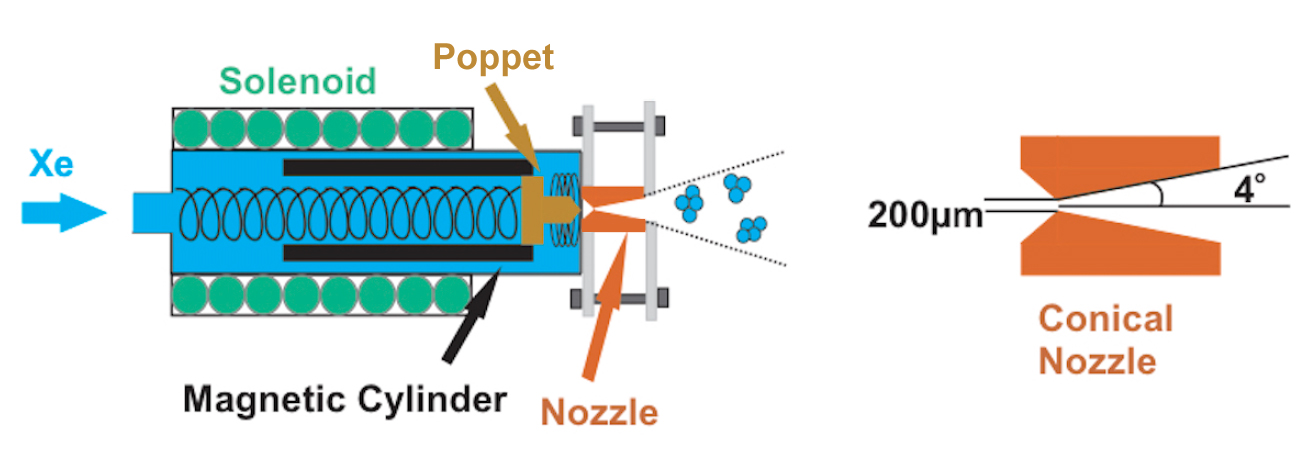
\includegraphics[width=1.00\textwidth]{images/parker-valve.jpg}
	\caption[Schematic of the Parker-Hannifin Series 99 valve.]{Schematic of the Parker-Hannifin Series 99 pulsed in-line valve and custom copper nozzle. The nozzle is clamped to the pulsed valve using an indium gasket to seal. The vespel poppet is attached to the magnetic cylinder and closes the valve. If a current is run through the solenoid, the valve actuates and opens. Adapted from \cite{Ferguson-2016-PhD}.}
	\label{fig:parker-valve}
\end{figure}
The helium source along with the xenon doping unit and the skimmers is depicted in Figure \ref{fig:Overview-Jetalignment}. Helium droplets are produced in a continuous free gas expansion using an electron microscope diaphragm as nozzle (Plano A0200P) that has a \SI{5}{\micro\meter} orifice and an orifice channel length of \SI{\sim 2}{\micro\meter} \citep{Gomez-2011-JCP}. The nozzle is cooled to cryogenic temperatures $\text{T}= \SI{5.8}{\kelvin}$ using a Sumitomo cold-head. The particle beam is defined by a first \SI{0.5}{\milli\meter} and a second \SI{1}{\milli\meter} diameter skimmer. As explained above, an adjustable slit system allows the definition the gas jet to single helium droplets. A doping unit is installed in the skimmer chamber of the helium source. It is a separate, smaller chamber in the skimmer chamber, where He-clusters can traverse through two smaller holes on each side. So, the gas load from the doping unit is mostly confined, which allows locally increasing the pressure of xenon to p$_{\text{du}}\leq \SI{0.3}{\pascal}$. The pressure is manually controlled using a leak valve. As schematically shown in Figure \ref{fig:pickupPrinciple}, the partial helium pressure is determined with a residual gas analyzer (RGA) opposite the helium source in the chamber that contains the AMO cluster source. The RGA pressure reading is used to determine the depletion $\tfrac{\Delta \text{p}_{\text{de}}}{\text{p}_{\text{de}}}$ (see Equation \eqref{eq:average-dopant}) of the helium clusters through the pickup of xenon atoms. A thorough alignment of the sources is necessary to overlap the particle beams such they traverse through all skimmers.%A summary of the alignment with a telescope and alignment laser is condensed in appendix \ref{sec:source-alignment}.
%
%
%
\subsection{Sample jet timing at LCLS}\label{sec:jet-timing}
%%%%%%%%%%%
% - explain timing
%%%%%%%%%%%%%%
\begin{figure}
	\centering
		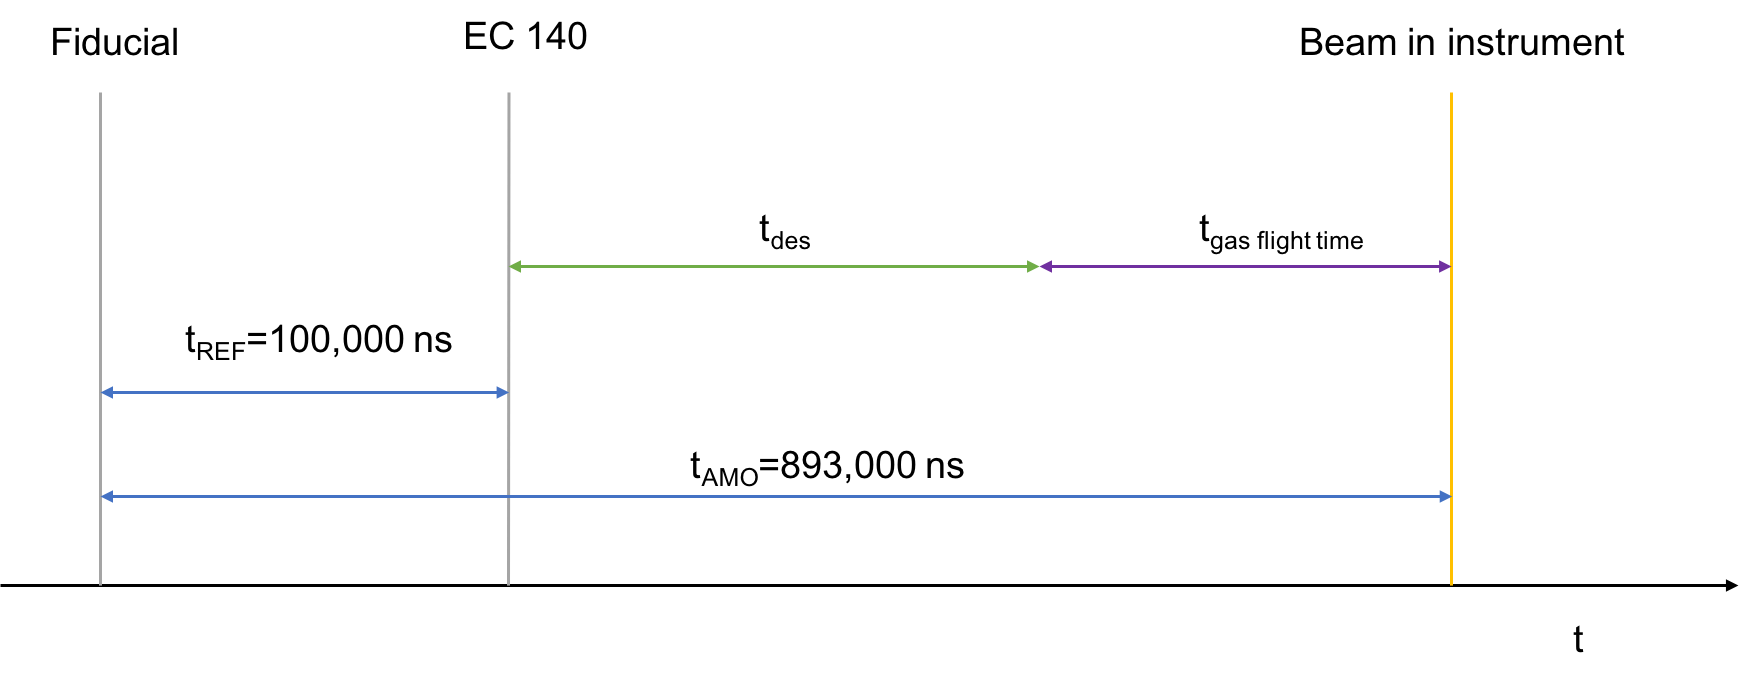
\includegraphics[width=1.00\textwidth]{images/LCLS-timing-schematic.png}
	\caption{Schematic of the LCLS event receiver (EVR) timing system.}
	\label{fig:LCLS-EVR-timing}
\end{figure}
Pulsed gas jets such as the one using the Parker solenoid valve require an electric trigger to open the valve at the right time such that the injected sample intercepts the light pulse. At LCLS, an event generator sends a fiducial, i.e., a clock signal with \SI{360}{\hertz}, and several event codes, e.g., at 120 Hz, to an event receiver (EVR) over a fiber network with a \SI{10}{\pico\second} precision \citep{Krejcik-2007-DIPAC}. The EVR processes these signals and supplies triggers to the components with a specific delay to an event code (EC). Figure \ref{fig:LCLS-EVR-timing} schematically illustrates the timing system. Following the schematic, the process starts with a fiducial and an event code, e.g., EC 140, is delayed by a time of event code x ($TECx$). After a certain time of the fiducial a LCLS pulse arrives. At the AMO instrument, this time\footnote{Times are in nanoseconds (ns) and in a format to comply with the LCLS interface.} is $t_{\text{AMO}}\approx$ \SI{893000}{\nano\second}. Each event code x has a slight variation in arrival time, $TECx$, with respect to the initial fiducial, as the timing signal has a ``clock rate'' of \SI{120}{\mega\hertz} only one EC can be sent every \SI{8.4}{\nano\second}. The LCLS control system automatically corrects for different $TECx$ by internally correcting the delay to a reference time $t_{\text{REF}}$ that corresponds to EC 140. EC 140 has a \SI{120}{\hertz} repetition rate and occurs only when an X-ray pulse is present. The reference time is artificially set to $t_{\text{REF}}=$ \SI{100000}{\nano\second}. We can gather the above considerations to establish a delay time to trigger a sample jet to coincide with a LCLS pulse. We note it as
\begin{equation}
t_{\text{delay}} = t_{\text{AMO}} - t_{\text{gas flight time}},
\label{eqn:sample-jet-delay-time}
\end{equation}
with $t_{\text{delay}}$ being the delay value for the LCLS EVR control system and $t_{\text{gas flight time}}$ the flight time of the sample from the gas source to the interaction region. As described in Section \ref{sec:homogenous-cluster} and Reference \citep{Miller-1988-Oxford}, the terminal velocity, $v_{\infty}$, of a sample from a supersonic jet is
\begin{equation}
 v_{\infty} \approx \sqrt{\frac{2\, R\, T_{0}}{m} \left(\frac{\gamma}{\gamma - 1}\right)},
\label{eqn:terminal-velocity}
\end{equation}
with the universal gas constant $R$, the temperature in the stagnation chamber $T_{0}$, and the ratio of specific heats $\gamma = \frac{c_{P}}{c_{V}}$, which is $\gamma = \frac{5}{3}$ for monoatomic gases such as rare-gases. The flight time of a certain gas can then be calculated by measuring the distance, $D$, between the source and the interaction region, thus $t_{\text{gas flight time}}=\frac{D}{v_{\infty}}$. The approach may be extended to approximate flight times of molecules, e.g., using the mass of CO, $m_{\text{CO}}=$ \SI{28}{\amu}, and also to gas mixtures, for example, the mass of a \SI{2}{\percent} xenon-131 and \SI{98}{\percent} helium-4 gas mixture can be estimated using a weighted average according to their relative contributions, thus  $m_{\text{HeXe}} =$ \SI{6.54}{\amu}. As convenience, the Table \ref{tab:terminal-velocities} shows terminal velocities of several rare gases at room temperature.\\[1\baselineskip]
\begin{figure}
	\centering
		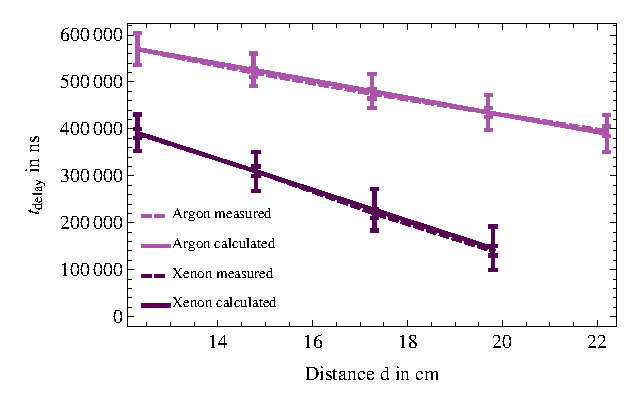
\includegraphics[width=0.70\textwidth]{images/gas-jet-flight-times.eps}
	\caption[Event receiver time delay at LCLS for supersonic gas jets.]{$t_{\text{delay}}$ as a function of the gas source distance to the interaction region. Xenon and argon has been used as sample gas in an Even-Lavie pulsed valve. The calculated delay values (solid lines) agree well with the measured delay times (dashed lines) to overlap the onset of the pulsed jet with the laser.}
	\label{fig:LCLS-delay-data}
\end{figure}
Figure \ref{fig:LCLS-delay-data} shows measured and calculated flight times using an Even-Lavie (EL) supersonic gas source\footnote{The EL-valve has the serial no.: EL 5 HRR NO 114.} instead of the earlier described Parker valve. The gas dynamics from an EL-source are similar to a Parker valve, but it has a very well-defined opening time and thus a well-defined gas jet. A typical opening time of the one used here is \SI{22}{\micro\second}, which can be time consuming to trigger properly without knowing $t_{\text{delay}}$. The data show very good overlap of the calculated delay times $t_{\text{delay}}$ from Equation \ref{eqn:sample-jet-delay-time} and the ion-yield maximum of the particle beam. The calculated flight times include an error margin, which can also be read as a recommended scan range. While the electric triggering and actual valve opening times may add errors on the microsecond time-scale, uncertainties in temperature $T_{0}$ and distance $D$ change delay times drastically.\\[1\baselineskip]
%
\begin{table}
\centering
\begin{tabular}{ | c | c | c | c | c | }
\hline
	\textbf{Sample gas} & \textbf{Helium} & \textbf{Neon} & \textbf{Argon} & \textbf{Xenon} \\ \hline
	$v_{\infty}$ & \SI{1745.5}{\meter\per\second} & \SI{780.6}{\meter\per\second} & \SI{512.0}{\meter\per\second} & \SI{305.0}{\meter\per\second} \\ \hline
\end{tabular}
\caption{Terminal velocities of some rare gases at room temperature, $T=\SI{293.15}{\kelvin}$.}
\label{tab:terminal-velocities}
\end{table}
%
Very long flight times can occur when heavy gases, such as xenon, are used or long distances, $D$, are necessary. If the flight times $t_{\text{gas flight time}} > t_{\text{AMO}}$ the system has to be delayed onto the next event as negative delays are not possible in the LCLS timing scheme. In this case, Equation \eqref{eqn:sample-jet-delay-time} can be rewritten to
\begin{equation}
t_{\text{delay}} = \frac{1}{f_{\text{rr}}} + t_{\text{AMO}} - t_{\text{gas flight time}},
\label{eqn:sample-jet-delay-time-next}
\end{equation}
with $f_{\text{rr}}$ being the repetition rate of the event code.
%
%
%
\section{Time-of-flight mass-spectrometer}\label{sec:TOF-spectrometer}
%%%%%%%%%%%%
%- fundamental aspects to the TOF detector\\
%- I'm hoping on some specific drawings from Timur / LCLS and SIMION simulations from Timur here.
%%%%%%%%%%%%%
An ion time-of-flight spectrometer was used in the interaction region to detect xenon and helium ions. A time-of-flight spectrometer uses electric fields to accelerate ions from the interaction region towards a detector. The detector unit often consists of a micro-channel plate (MCP) that allows recoding an arrival signal and calculating the time-of-flight (TOF) of the ions. The following considerations connect the time-of-flight to ions with a specific \textit{mass-to-charge ratio} \citep{Stephens-1946-APSSpring}.\\[1\baselineskip]
%
In the first stage, the ions are accelerated from the interaction region towards the detector. Here, the electric potential energy is converted into kinetic energy
\begin{align}
q U &= \frac{1}{2}m \left(\frac{d_{1}}{tof_{1}}\right)^{2},\\
tof_{1} &= \sqrt{\frac{m}{2qU}}\cdot d_{1},
\end{align}
with $q$ being the elementary charge of the ion, $U$ the voltage difference, $d_{1}$ the distance between the interaction region and spectrometer, $m$ is the mass of the ion, and $tof_{1}$ is the time-of-flight in the acceleration stage. The ions then travel through a drift tube of length $d_{2}$ that is field free. As the velocity remains constant, we can write down
\begin{equation}
tof_{2} = \sqrt{\frac{m}{2qU}}\cdot d_{2},
\end{equation}
with $tof_{2}$ being the time-of-flight in the drift tube. The total flight time can then be written as
\begin{align}
t_{\text{tof}}=tof_{1}+tof_{2}=\sqrt{\frac{m}{2\, q\, U}} \left(d_{1}+d_{2}\right),\intertext{In a typical experiment, all values aside from $m$ and $q$ can be considered constant. Therefore, we may note the time-of-flight in its well known dependency, as}
t_{\text{tof}} \propto \sqrt{\frac{m}{q}}.
\end{align}
%As the spectrometer is a cylindrical system, the time-of-flight denotes the final position on the detector and vice versa. 
%Therefore, $t_{\text{tof}} \propto\sqrt{\frac{m}{q}}$ of the ensemble of ions in the interaction region upon interaction with an X-ray pulse.
In specific cases, where atoms become ionized and their kinetic energy, $E_{kin}$, is $E_{kin}=0$, the spectrometer records narrow peaks that are spaced according to their mass-to-charge ratio. However, atomic ions usually start with a kinetic energy, $E_{kin}\neq 0$, such that the time-of-flight is altered and the signal peak structure is broadened. If molecules or clusters become ionized, fragments have additional translational energy resulting from dissociation of a metastable ion measured relative to the center-of-mass, which is often referred to as kinetic energy release \citep{Murray-2013-IUPAC}. This leads to additional broadening of the signal peak structure.\\[1\baselineskip]
%Atomic ion time-of-flight data typically exhibits a distinct peak structure while the signal from clusters is strongly broadened due to kinetic energy release from collective effects. 
%For this thesis, the time-of-flight data is used to measure the level of ionization and kinetic energy release of ions to quantify the degree of sample damage upon irradiation with a LCLS pulse.
\begin{figure}
   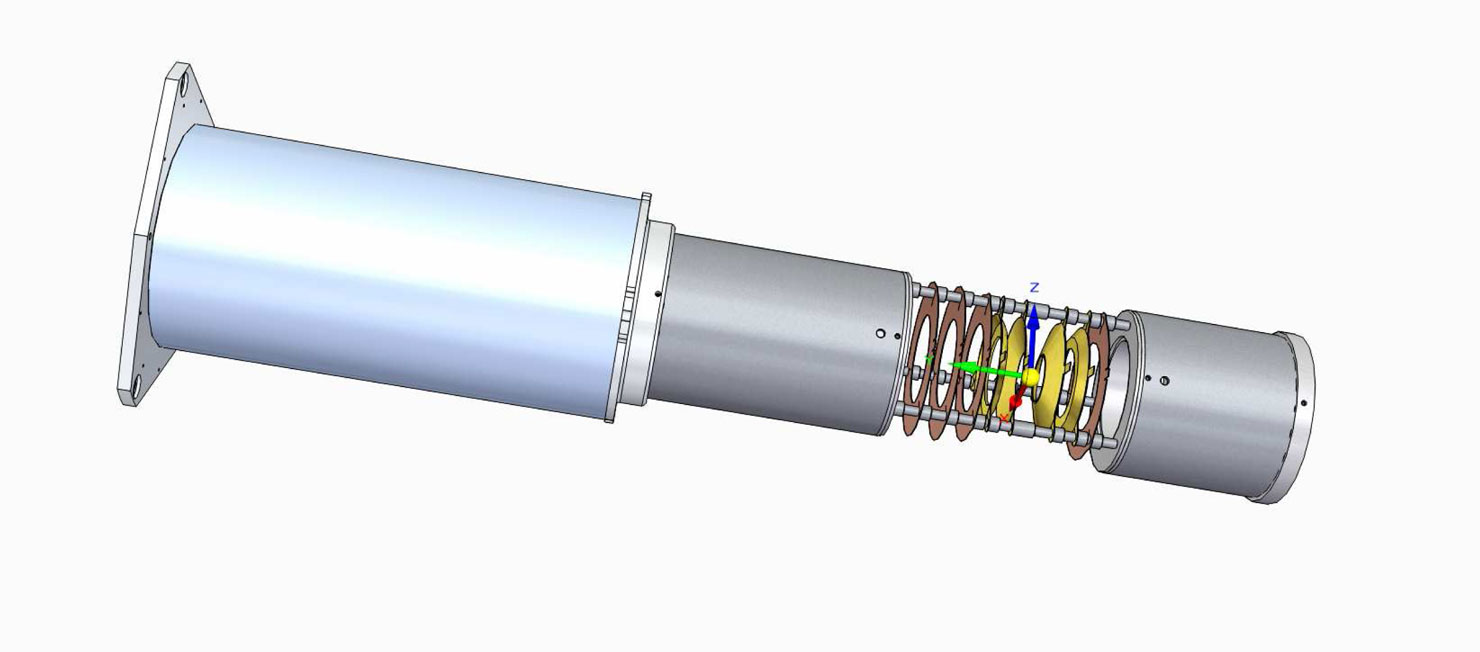
\includegraphics[width=1.\linewidth]{images/spectrometer.jpg}
    \caption{Drawing of the time-of-flight spectrometer.}
\label{fig:spectrometer-detail}
\end{figure}
The time-of-flight spectrometer used in this thesis experiment is depicted in Figure \ref{fig:spectrometer-detail}. It is a double sided spectrometer for electron and ion detection. %The conical lenses restrict the acceptence of energWith $\pm 5$ keV power supplies, ions can be detected up to kinetic energies of 50 eV with a time-of-flight resolution of 100 ps \citep{Ferguson-2015-JSR}. If only the ion side is used, ions with kinetic energies of up to 100 eV can be detected. The use of $\pm 10$ keV power supplies allows a detection of kinetic energies up to 150 eV. Electrons can be measured up to kinetic energies of 150 eV using $\pm 5$ keV power supplies, 300 eV if only the electron side is used and 400 eV when using $\pm 10$ keV power supplies. Ions and electrons can be detected whether they are emitted in any direction, in other words the spectrometer has a $4\pi$ solid angle collection \citep{Osipov-2013-PC}.
\begin{figure}
   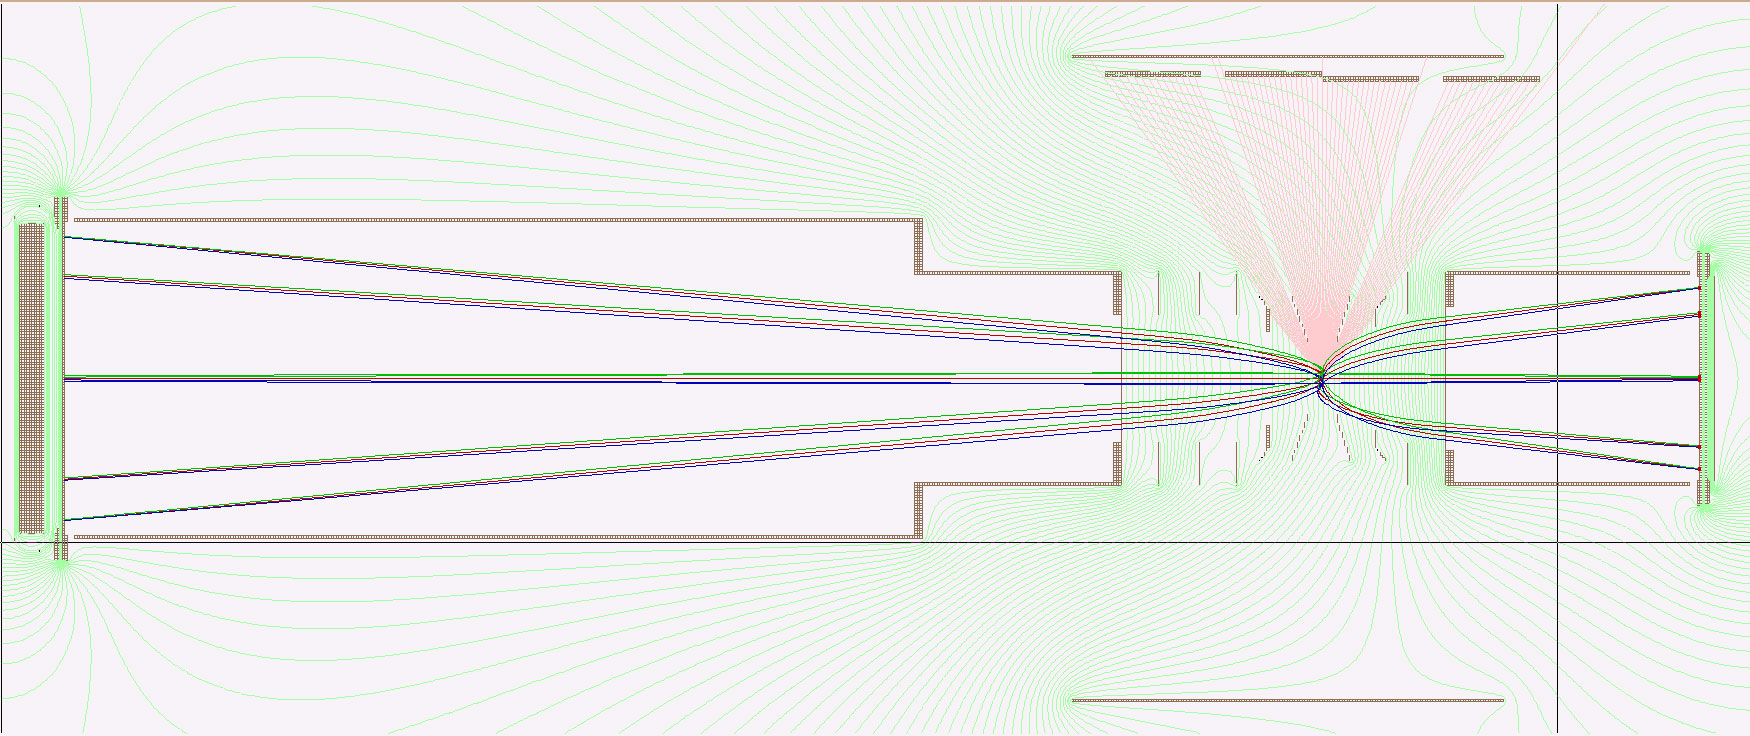
\includegraphics[width=1.\linewidth]{images/simion.jpg}
    \caption[Sideview of the spectrometer showing ion, electron and photon trajectories.]{Sideview of the spectrometer showing ion, electron and photon trajectories upon interaction with LCLS. The image was created with SIMION. From \cite{Osipov-2013-PC}.}
\label{fig:simion}
\end{figure}
A side view of the spectrometer can be found in Figure \ref{fig:simion}. In this schematic, ion, electron and photon trajectories upon interaction with a LCLS pulse have been simulated using SIMION \cite{Osipov-2013-PC}. A conical lens stack avoids casting a shadow on the pnCCD detectors (top of schematic). The applied voltages in the experiment can be found in Table \ref{tab:tof-volategs}. Only ion spectra have been recorded but in the experiment, the electron side is powered to have unperturbed electric fields across the interaction region.
%
\begin{table}
\centering
\begin{tabular}{ | c | c || c | c | }
\hline
	\textbf{Ion-side Connection} & \textbf{Voltage in V} & \textbf{El. Side Connection} & \textbf{Voltage in V} \\ \hline
	MCP Front & -2600 & MCP Front & 200 \\ \hline
	MCP Back & 5 & MCP Back & 2200 \\ \hline
	Holder & 200 & Phosphor & 3000 \\ \hline
	Conical lens 70deg & -923 & Holder & 6000 \\ \hline
	Conical lens 53deg & -1393 & Conical lens 70 deg & 500 \\ \hline
	Flat lens \#1 & -1490 & Conical lens 53 deg & 1370 \\ \hline
	Flat lens \#2 & -1564 & Flat lens & 1940 \\ \hline
	Flat lens \#3 & -1639 & Flight tube & 2736 \\ \hline
	Flight tube & -1714 & - & - \\ \hline
\end{tabular}
\caption{Applied voltages to the time-of-flight spectrometer (ion side use only).}
\label{tab:tof-volategs}
\end{table}
%
%
%
\section{X-ray focus characterization}\label{sec:focus-characterization}
%
A focus characterization is usually performed before X-ray diffractive imaging experiments to optimally focus the X-rays at the desired interaction region. Two focus characterization methods are described here: one, using a TOF spectrometer; and two, being a so-called imprint study.
%
%
%
\subsection{Focus characterization using a TOF spectrometer}
%
\begin{figure}
	\centering
		a)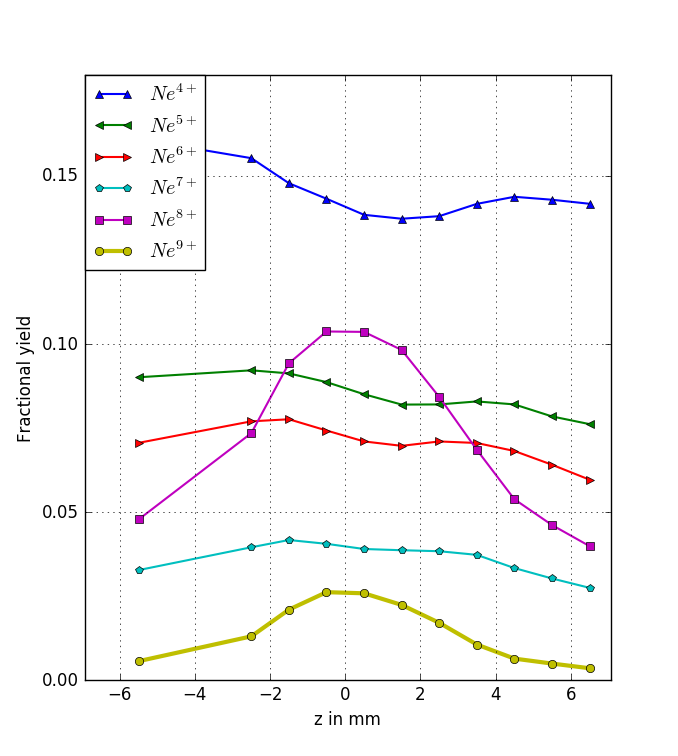
\includegraphics[width=0.40\textwidth]{images/Focus-z-scan.png}
		b)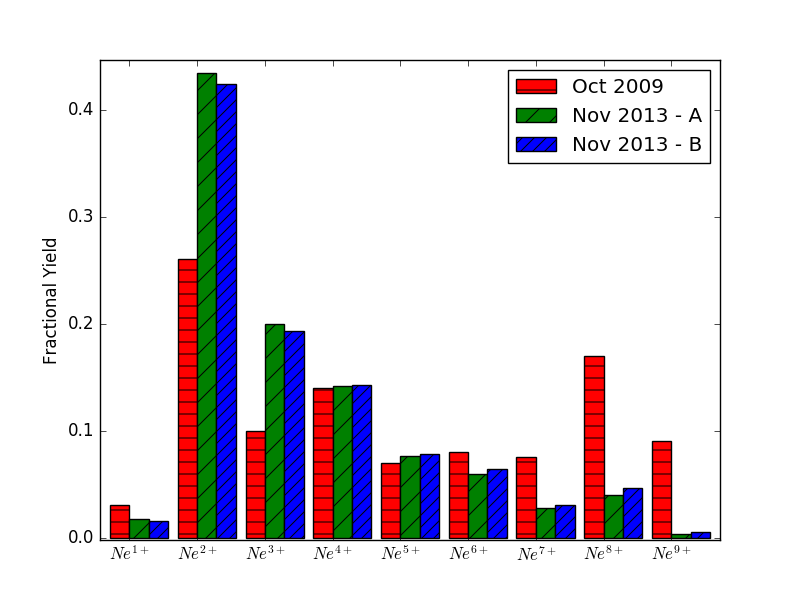
\includegraphics[width=0.54\textwidth]{images/Focus-Fractional-Yield.png}
	\caption[Focal spot analysis using a time-of-flight ion spectrometer.]{a) Atomic neon charge state yield from TOF as a function of $Z$-position, relative to optimal focus position $\text{Z}=0$. $Z=\SI{0\pm 1}{\milli\meter}$ is a favorable length for sample injection. b) Comparison of atomic neon charge state yield from TOF for different cases: red, experimental data from October 2009 with 4 blades (S) opened; green, experimental data from November 2013 with (S) closed; blue, Experimental data from November 2013 with (S) opened.}
	\label{fig:Focus-z-scan}
\end{figure}
%
For a focus characterization using a TOF spectrometer, the experimental chamber is usually filled with a well known gas, for example, neon, such that the pressure inside the experimental vacuum chamber is on the order of \SI{e-4}{\pascal}. The TOF spectrometer or the focal point are then moved with respect to each other and ion time-of-flight data is recorded. The left panel in Figure \ref{fig:Focus-z-scan} shows a focus characterization, where a TOF spectrometer was driven along the $Z$-axis on which the X-ray focus was placed. The fractional neon ion-yield per charge state is plotted as a function of the spectrometer's $Z$-position. The data show that a \SI{2}{\milli\meter} region centering around the focal plane at $Z=$ \SI{0}{\milli\meter} is most useful for experiments requiring high X-ray intensities. The right panel of Figure \ref{fig:Focus-z-scan} compares the fractional neon ion-yield at the optimal focus position from November \num{2013} \citep{Bucher-2016-Unpublished} to October \num{2009} \citep{Doumy-2011-PRL} using \SI{\sim 1.25}{\kilo\electronvolt} photons and comparable pulse energies. The comparison reveals that high-charge states of neon, for example, $Ne^{8+}$ and $Ne^{9+}$, are less abundant, which can be attributed to the deterioration of the optics over the first years of operations.
%
%
%
\subsection{Focus characterization via an imprint study}
%
\begin{figure}
\begin{tabular}{ccc}
  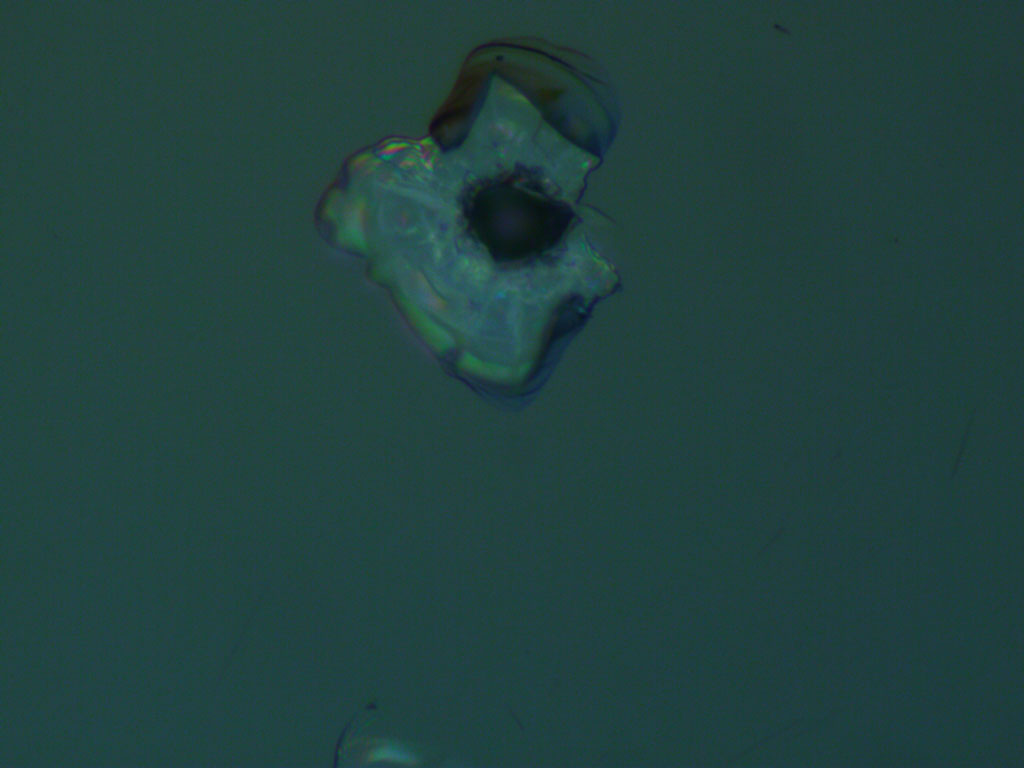
\includegraphics[width=0.25\textwidth]{images/imprints/image0025.jpg} & 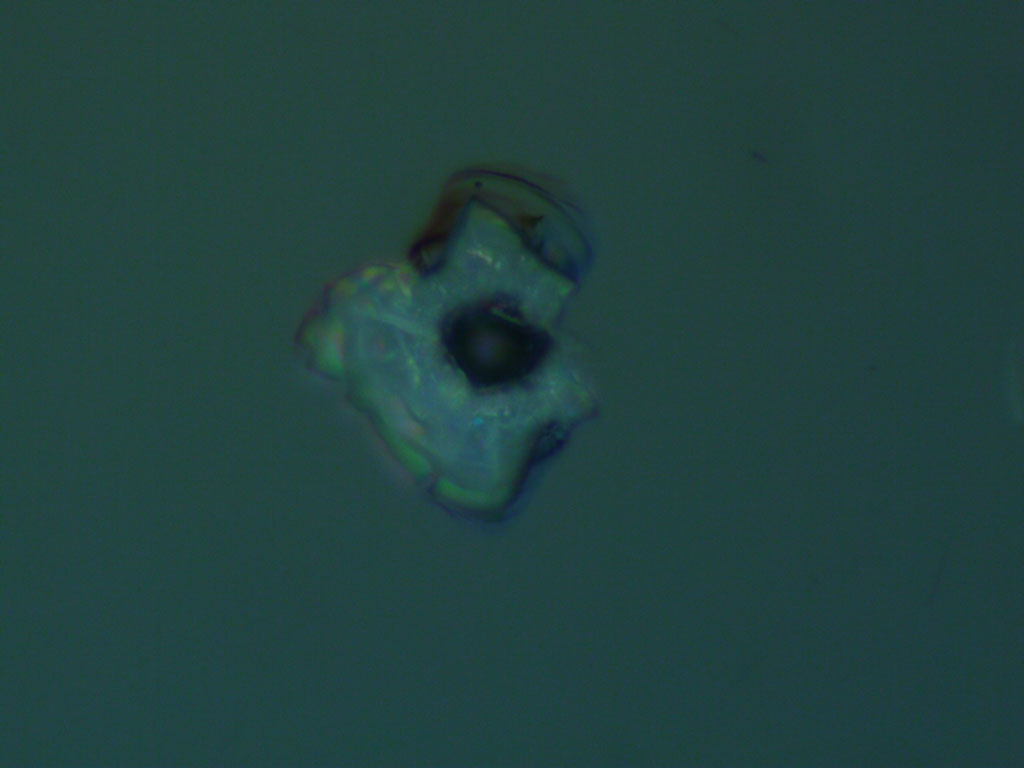
\includegraphics[width=0.25\textwidth]{images/imprints/image0026.jpg} & \multirow{3}{*}[1.5cm]{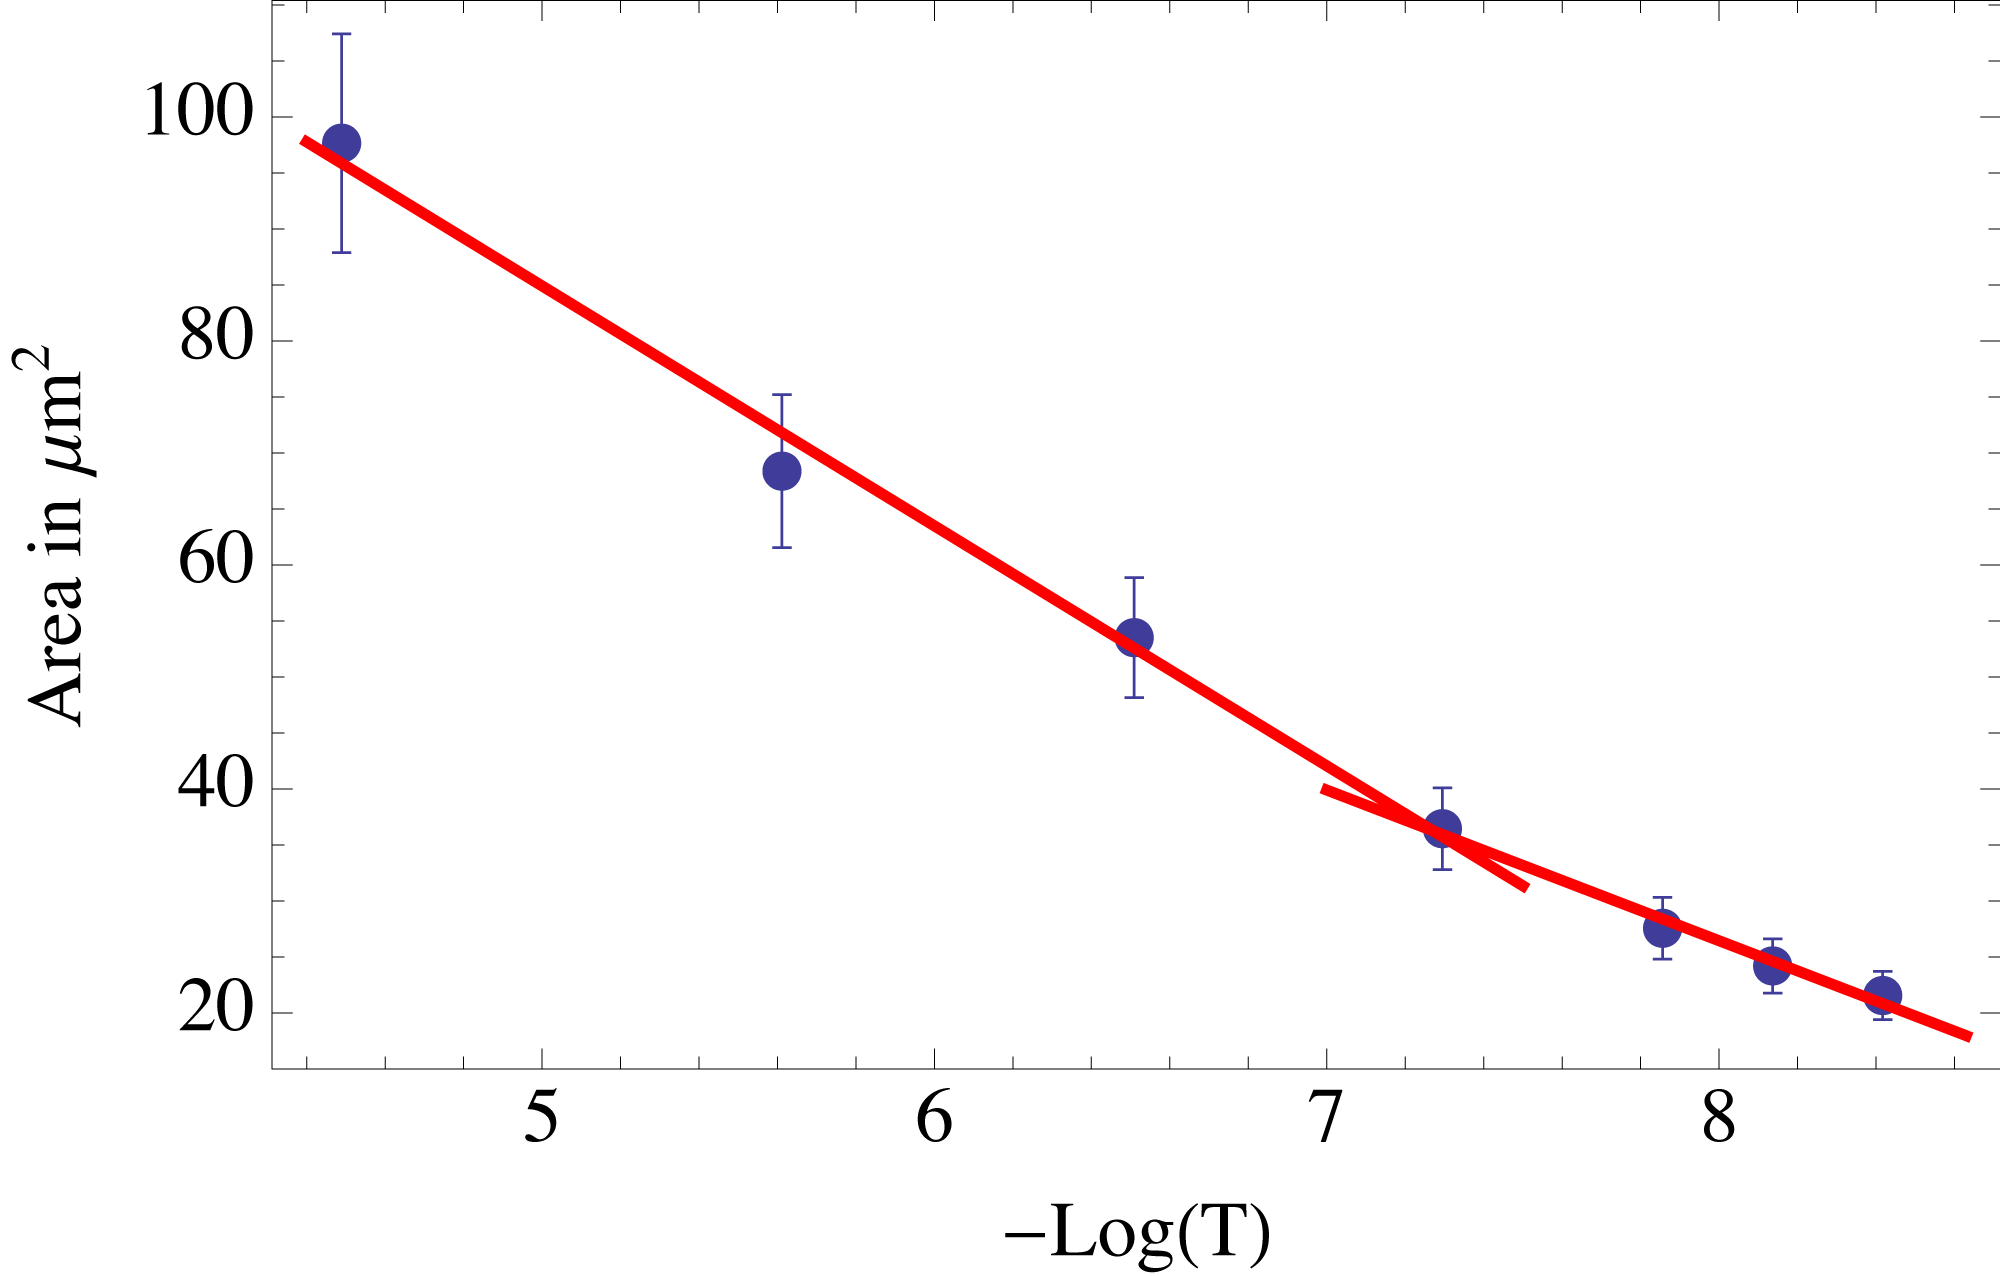
\includegraphics[width=0.49\textwidth]{images/imprints/analysis.png}} \\
a) & b) & \\[6pt]
 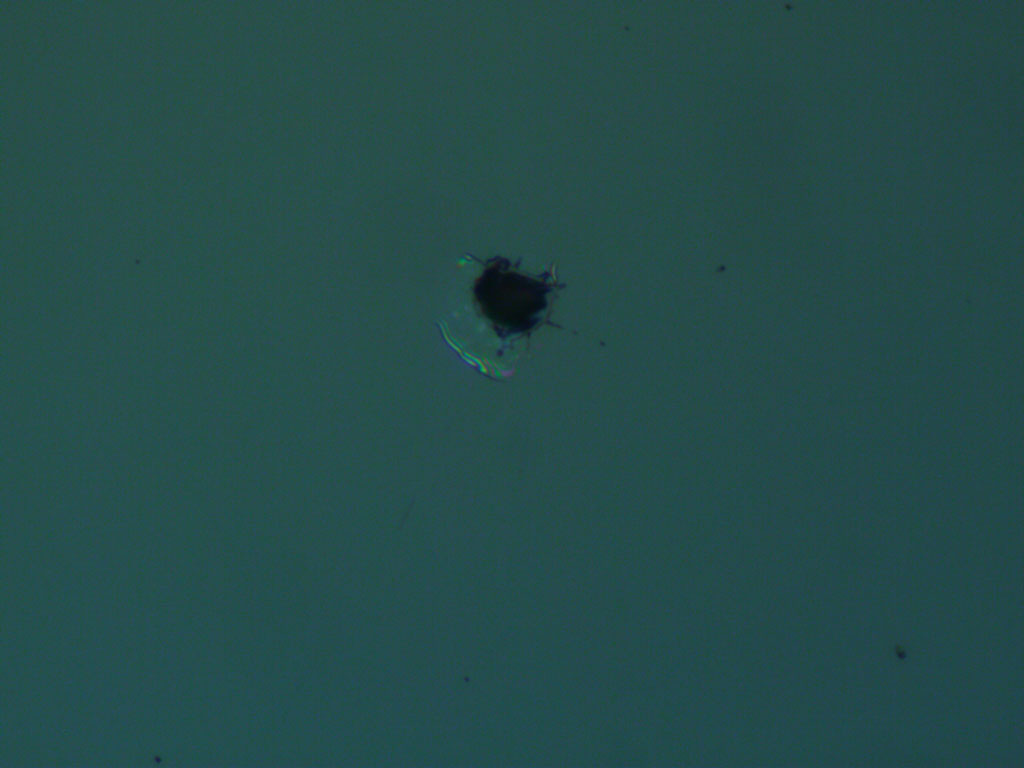
\includegraphics[width=0.25\textwidth]{images/imprints/image0027.jpg} & 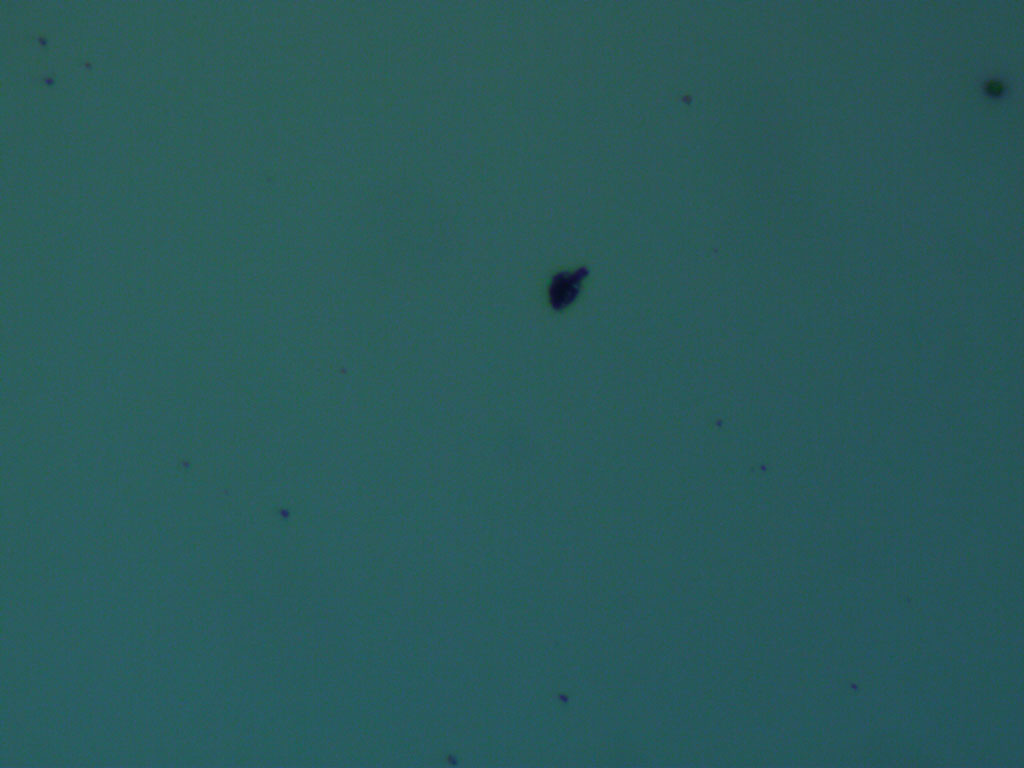
\includegraphics[width=0.25\textwidth]{images/imprints/image0028.jpg} &  \\
c) & d) & e)
\end{tabular}
\caption[Focal spot analysis via an ex-situ microscope imprint study.]{a)-d) Ex-situ microscope imprint study of a lead tungstate\index{lead tungstate} sample that was irradiated with single, \SI{1600}{\electronvolt} LCLS pulses at different gas attenuation. e) Non-linearity in Liu plot \citep{Liu-1982-OptLett} due to LCLS's multi-gaussian beam profile. The approximate FWHM$\approx$ \SI{3.4}{\micro\meter} is determined from the slope of the linear fits.}
\label{fig:imprint-study}
\end{figure}
%
In an imprint study, a target, typically a lead tungstate ($\text{PbWO}_{4}$)\index{lead tungstate} window, is placed at the desired interaction region on a motorized stage. The X-ray focus is then moved and for each step at least one X-ray pulse should be shot at the target. The target is then moved slightly since the X-rays point at the same spot and the procedure repeated. This process should be repeated at various X-ray beam attenuation, as we will see below. Figure \ref{fig:imprint-study} shows exemplary data from an imprint study. The $\text{PbWO}_{4}$-target is studied using an optical microscope and typical imprint images are shown in the panel a) to d). Here the target was illuminated with LCLS X-ray pulses at \SI{1600}{\electronvolt} at various transmission values, $T$. The crater sizes vary according to the X-ray peak fluence and we shall derive in the following the correlation between crater size and the full-width at half-maximum (FWHM).\\[1\baselineskip]
%
Let us describe the energy fluence, E(R), of the X-rays as
\begin{equation}
E(R) = E_{0} e^{\frac{-R^{2}}{2 \sigma^{2}}},
\end{equation}
with the radial coordinate $R$, a characteristic radius $\sigma$, and the peak fluence $E_{0}$. Typically, $\sigma$ stays a constant beam parameter, which is typically set by the optimal focus position of the KB-optics and thus does not affect the crater area. The crater area changes due to varying the peak fluence, $E_{0}$. As $E_{0}$ increases, more and more of the target is irradiated with power densities above the damage threshold such that larger craters form. We can measure the peak fluence, $E_{0}$, through to the pulse energy, $E_{p}$, which is measured with the gas detector. Let us explicitly note their proportional dependency, $E_{0}\propto E_{p}$. Now, we can express the peak fluence more conveniently in terms of the pressure, $p$, in the gas attenuator
\begin{equation}
\log(E_{0}) = \log(E_{\text{in}})+\log(T)= -p \cdot c + \text{const.},
\label{eq:gaussian-beam-imprint}
\end{equation}
with the incident peak fluence at the gas attenuator $E_{in}$ and the transmission $T$. In the gas attenuator, the transmission is $T=e^{-p \cdot c}$ and a constant $c$. The constant $c$ can be derived from Reference \citep{Henke-1993-ADNDT}. For the LCLS attenuator filled with nitrogen gas (N$_{2}$) over its \SI{4.1}{\meter} length at \SI{1600}{\electronvolt} photon energy, $c\approx$ \SI{4.20890737e-3}{\per\pascal}. We can further approximate the crater surface area using a circle. The area then is $\pi r_{0}^{2}$, with the crater radius $r_{0}$. As shown in Reference \citep{Liu-1982-OptLett}, $r_{0}^{2}=2\sigma^{2}log(\tfrac{E^{2}_{0}}{E_{0}^{1}})$, with $E_{0}^{1/2}$ being the peak fluence at two different attenuation levels. Thus, the slope of a linear fit between the two points $E_{0}^{1/2}$ is $2 \pi \sigma^{2}$. The FWHM $=2\sqrt{2 ln(2)}\sigma$. The right panel of Figure \ref{fig:imprint-study} shows the crater-area as a function of $-log(T)= p \cdot c$, which is often referred to as a Liu's plot. The data points are fitted with two linear fits, which indicate non-linearities that come from a multi-Gaussian beam-profile, which is often called a super-Gaussian beam-profile \citep{Chalupsky-2010-OE,Chalupsky-2013-OE}. The FWHM can be determined from the slope of the linear fit at smaller transmissions and is $\text{FWHM}\approx \SI{3.4}{\micro\meter}$ using the exemplary data. The LCLS parameters in the experiment of this thesis are different to the above exemplary data and are summarized in Table \ref{tab:beam-params}.
%
%
%
%\newpage
\chapter{Methods}\label{ch:methods}
Let us continue by conservatively estimating  how much data is produced when using the LAMP end-station with both pnCCD detectors in use at a $120$hz. Each pnCCD produces 120 images per second, each image is in a 32 bit per pixel format such that an image is vaguely $4$ megabyte in size. So, every minute the front \& rear pnCCD produce approximately $60$ gigabyte of data. To analyze these vasts amount of data an extensive set of methods and optimized algorithms is required. This chapter is devoted to illuminate the analysis methods used in the present thesis.\\
The chapter is organized as follows, section \ref{sec:LCLS-computing} describes the general LCLS computing environment to establish an overview of the hard- and software capabilities. Section \ref{sec:pnccd-corr} discusses corrections that are applied to the raw pnCCD images. In section \ref{sec:hitfinding}, several hitfinding methods are being evaluated. Section \ref{sec:phase-retrieval} goes over used phase-retrieval algorithms. Finally, section \ref{sec:2d-simulations} discusses simulations of 2D projections of spheres and corresponding diffraction patterns.
%
%
%
\section{The computing environment at LCLS}\label{sec:LCLS-computing}
%%%%%%%%%%%%%%%%
%- Include basics around the PSANA interface\\
%- For example how the date is converted, then stored and\\
%- the analysis opportunities along the way
%- I think this will be a longer subsection since a lot of my work went into this and I'm regularly contacted about it.
%- Short introduction what we have to go through\\
%- Reminder of detectors and analysis environment
%%%%%%%%%%%%%%%%
\begin{figure}
	\centering
		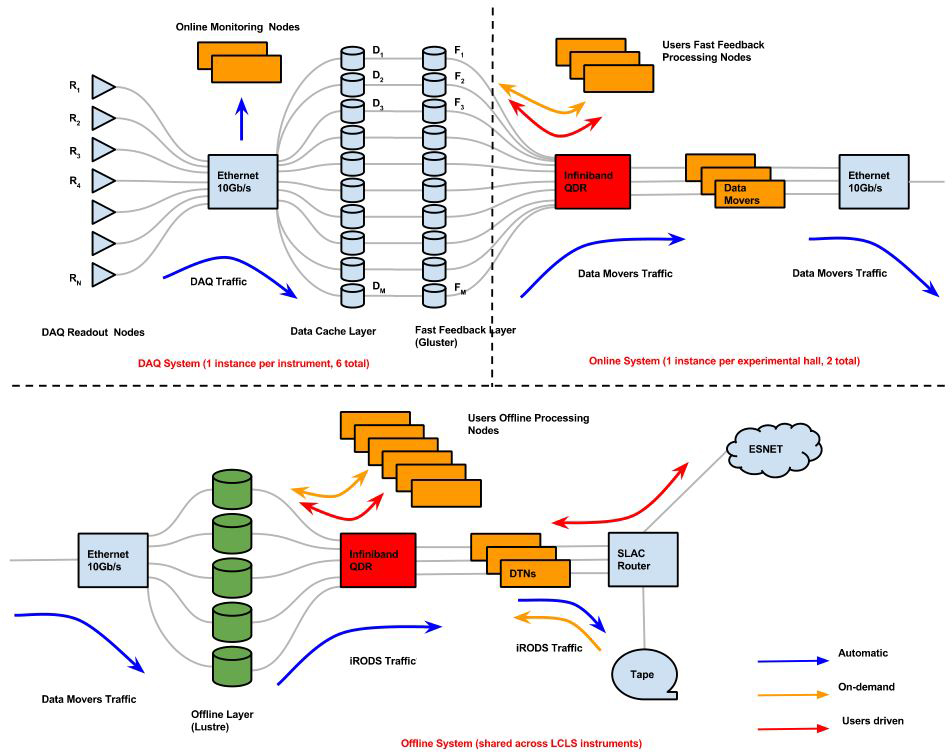
\includegraphics[width=1.00\textwidth]{images/daq-architecture.JPG}
	\caption[Diagram of the computing environment at LCLS and DAQ traffic.]{Diagram of the computing environment at LCLS and DAQ traffic. The recorded data is exchanged through Ethernet and after digitization, is stored on a cache and FFB cluster, where psana computer have access to the online environment during the experiment. Eventually, the data is moved to the more permanent offline environment, where data can be analyzed on psana computers or through a load sharing facility. See more in text. From \citep{Amadeo-2016-SLAC}}
	\label{fig:daq-architecture}
\end{figure}
As estimated above, the vast amounts of data generated by many detectors are unhandy to handle by a single group of scientists that perform experiments at LCLS. For this reason the LCLS data acquisition (DAQ) group has incorporated many detectors, for example the the pnCCD and Aqciris digitizer, into their framework. All data taken at LCLS is stored in the LCLS computing environment, where the data can also be analyzed. As indicated in figure \ref{fig:daq-architecture}, DAQ readout nodes send the data traffic via Ethernet to a short-term cache and fast feedback (FFB) layer. While the data is being transferred, online monitoring nodes are able to 'see' a fraction of the live (online) data and run analysis. With a delay of a few ten seconds, the FFB nodes can be used to run analysis on the full data stream using parallelization, thereby having 'online' and 'offline' data access. Eventually the data is being moved to the 'offline' layer, where the data is managed by an integrated Rule-Oriented Data System (iRODS). The data is stored in .XTC file containers and it can also be accessed from outside SLAC (Router \& ESNET). The stored data has certain storage quotas and times. In brief, there is a 6 months short-term storage without quota limitations and a two-year medium-term storage with a storage quota of $10 000$ Giga-Byte. After that, the data is automatically stored for at least 10 years on magnetic tape (long-term storage) and can be restored upon request. A web interface is provided by the DAQ group to simplify and automate the data-handling and logging process. The short- and medium term storage solutions can also be used to analyze the data using the psana-framework to access data and to perform computations on the psana computer cluster with over 1000 CPU cores. A load sharing facility (LSF) allows the scheduling of (parallelized) batch jobs. The psana-framework can be interacted with python 2.7. The interacting python script calls functions within the psana-framework that are programmed in C(++), for example detector calibrations. Psana allows parallelization via MPI and it is therefore possible to analyze many events (LCLS pulses) simultaneously. Also complex analysis is able process at the rate of the incoming data using MPI, when the FFB is used. Python scripts can be written for 'online' or 'offline' analysis and are of similar syntax.\\
For LCLS-II \citep{Amadeo-2016-SLAC}, the analysis and data-access scheme is designed to be similar to figure \ref{fig:daq-architecture} with the exception of the online monitoring nodes. It is therefore recommended to build analysis schemes that are based on psana and use the FFB for online analysis, which can then be adapted easily for offline analysis as well. A quick introduction on how to use psana can be found in the appendix \ref{sec:python-example}, where a few examples from the LCLS DAQ group are condensed.
%
%
%
\section{pnCCD photon detectors}\label{sec:pnccd-corr}
%%%%%%%%%%%%%%%%
%- Describe signal on the pnCCDs\\
%- Calibrations and corrections - use LAMP paper\\
%- single hits\\
%- multiple hits
%%%%%%%%%%%%%%%%
\begin{figure}
	\centering
		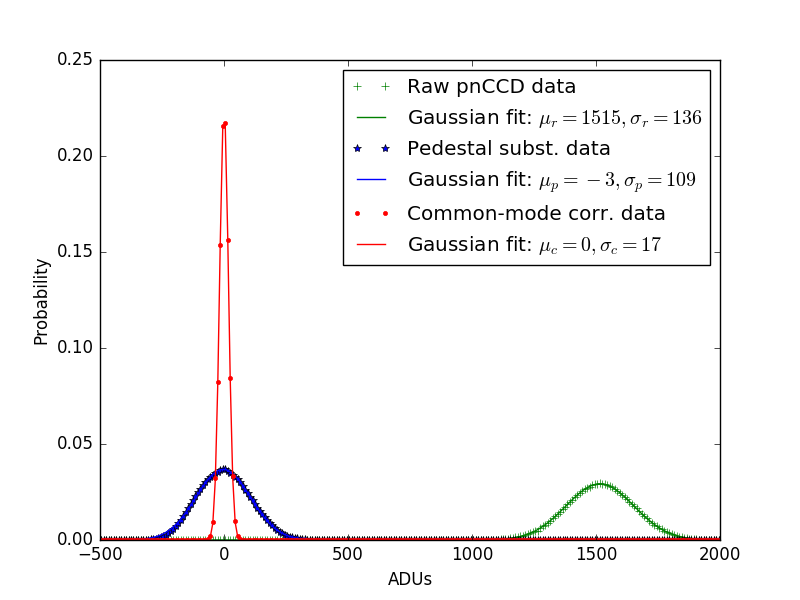
\includegraphics[width=0.80\textwidth]{images/pnCCD-electronic-noise.png}
	\caption[ADU histograms from electronic noise of not illuminated pnCCDs in highest gain mode.]{ADU histograms from electronic noise of not illuminated pnCCDs in highest gain mode. The green, plus symbols reflect a histogram of ADU values from raw electronic noise of pnCCD pixel. One can see that the noise is set off zero at $\mu_{r}=1515$ ADU and has a standard deviation $\sigma_{r}=136$. The same data shifts to the blue stars are after applying the pedestal subtraction. The noise is centered around $\mu_{p}=-3$ and it's standard deviation is reduced to $\sigma_{p}=109$. For the red  data points, the common-mode corrections have additionally been applied. Now, the noise is well-centered at $\mu_{c}=0$ ADU and $\sigma_{c}$ is significantly reduced to $17$. Note again, that this is an ADU histogram of purely electronic noise in highest-gain imaging mode.}
	\label{fig:pnCCD-electronic-noise}
\end{figure}
Before the pnCCD detectors can be used to take data, it is good practice to apply corrections to the raw detector image in order to cope with electronic noise. Since these corrections are used often, the LCLS detector and DAQ group has implemented a calibration manager tool\index{psana!calibman}\footnote{The calibration manager tool 'calibman' can be found in the 'psana' software package. More information under \url{https://confluence.slac.stanford.edu/display/PSDM/Calibration+Management+Tool} (Oct 2016)} that provides the necessary algorithms and helps with the procedure of applying image corrections and more. We discuss the two most often used corrections next. One, corrects for the electronic noise pedestals\index{pnCCD!pedestal correction} (levels) of each pixel, and two, accounts for common modes\index{pnCCD!common mode}, e.g. artifacts from the read-out electronics that appear for the pnCCD in columns.\\
%
The effects of applying these corrections are illustrated in figure \ref{fig:pnCCD-electronic-noise} through a set of histograms. The histogram bins are showing ADU values from dark pnCCD images in highest gain. The green curve shows the ADU values of a raw detector image where no corrections have been applied, i.e. the electronic noise response from the chip has a standard deviation of $\sigma_{r}=136$. Note, that there is also a significant offset of the distribution from 0 to $\mu_{r}=1515$ ADU. The blue curve shows the same data but is using the pedestal corrections found in 'calibman'. The pedestal corrections reduce the noise slightly to $\sigma_{p}=109$ ADU, and as expected, the pedestal corrections drastically move the normal distribution to be centered around $\mu_{p}=-3$. Finally, the red curve is also the same data than the green curve but includes pedestal and common-mode corrections. The corrected read-out modes drastically improve the standard deviation to $\sigma_{c}=17$ and slightly move the mean to $\mu_{c}=0$.\\
As a guideline, the pedestal corrections should be always used to account for the mean offset. The common-mode calibration, however, should be tested before applying. The algorithm that determines common-modes needs to find a baseline and therefore needs pixel with no signal in each row and column. In single-particle imaging the detector is illuminated in (almost) every pixel. Then the common-mode correction algorithm may treat real signal as noise and fail to find a common baseline.\\
In the present thesis, pedestal and common-mode correction has always been applied on the front detectors, as these pixel hold mostly signal from single photons. The rear pnCCD uses the pedestal correction but corrects common-modes only above a certain, conservative threshold. See figure \ref{fig:pnCCD-image-aligned} for the visible effect on front detector (large, top/bottom arrays) and rear detector (small, centered array).\\
%
%
%
%\subsection{Signal analysis}
%- Present data from 1500eV photon energy on Xe backfilled chamber with the pnCCDs in spectroscopy mode to argue that the pedestal and offset corrections are enough to correct for fluoresence.\\
%- Masked areas in image
%%%
%
%
%
\subsection{Combining multiple pnCCD detectors}\label{sec:combination-of-images}
%%%%%%%%%%%%%%%%%%%%%%%%%
%- Explain how I combined pnCCD detectors to perform reconstructions on it.\\
%- Can reuse material from the LAMP pnCCD paper
%%%%%%%%%%%%%%%%%%%%%%%%%
In order to maximize resolution, it is most useful to combine multiple pnCCD detector modules into one image. While this is a simple task on itself, it becomes more complex, when the combined images need to undergo a phase-retrieval process that use fast Fourier transformations (FFTs). In fact, it has not yet been shown in single-particle imaging that it is possible to retrieve a real space image from multiple detectors in different planes.
%One of the reasons is, that the samples, that were studied in recent years were comparably large, e.g. viral samples of a few hundred nanometer radius that don't scatter to wide angles. Therefore, in many experimental setups, the distance of this detector is then set to fill the detector planes appropriately to the scattering of the sample. In other words, there was no incentive of combining detectors.
The reason for this is that thus far there was little incentive of merging multiple detectors. Until recently, typical samples were on the order of several hundred nanometers in diameter such that little signal could be detected at large scattering angles. With the intensities provided by LCLS and the single-particle imaging capabilities of the LAMP end-station objects that are smaller than a hundred nanometer in diameter can be studied.
%To cover this variety in object size, LAMP's front pnCCD detector can move along the z-axis and can cover wide scattering angles from smaller objects and LAMP's rear pnCCD detector covers the usual small angles scattering from larger objects. Once the detector is set to cover most scattering angles, one finds that the dynamic range and photon sensitivity becomes a limiting element.
Besides the ability to cover larger scattering angles, multiple detectors can be operated in different gains and still be combined efficiently. For the pnCCD, this allows not only an increase in dynamic range but improves the signal-to-noise.\\
Let us now describe the process of combining diffraction images, while simultaneously preparing them for the inverse problem of phase-retrieval. The discussion now follows the code shown in appendix \ref{sec:combination-of-detectors-code}. The input for the following procedure are two pnCCD images. The images should be pedestal corrected and if possible common-mode corrected. Analysis of the electronic noise determines an cutoff or offset between signal-to-noise for each image (see left figure \ref{fig:pnCCD-histogram} and \ref{fig:pnCCD-electronic-noise}). At this step it is also convenient to account for different detector gain settings using the table \ref{tab:gain-modes} and normalize detector distances using, e.g., the following equation to correct the signal to the front pnCCD plane
\begin{equation}
\text{image}_{\text{normalized}} = \text{image}\cdot \frac{\text{gain}_{\text{front}}}{\text{gain}_{\text{rear}}} \cdot \frac{\text{distance}_{\text{rear}}^{2}}{\text{distance}_{\text{front}}^{2}}
\end{equation}
The pnCCD front top and bottom module are placed in an enlarged array to reflect the real geometry in the plane of the front pnCCD. We can now translate this with pixel constructed geometry to use the more general scattering angle $\Theta$
\begin{equation}
\Theta = \arctan\left(\frac{\sqrt{\text{pixel}_{\vec{x}}^{2}+\text{pixel}_{\vec{y}}^{2}}\times a}{d}\right),
\label{eqn:scattering-angle}
\end{equation}
with $pixel_{\vec{x}}$ and $pixel_{\vec{y}}$ being the length of the pixel array from the beam along the X- and Y-axis, respectively. We can use this information to further generalize the matter and attribute a scattering vector $\vec{Q}$ to each pixel
\begin{equation}
\vec{Q} = 4 \pi \frac{\sin\left(\frac{\Theta}{2}\right)}{\lambda},
\label{eqn:q-vector}
\end{equation}
with $\lambda$ being the wavelength of the scattered photons. We can now add the signal from the rear pnCCD to the enlarged array, while using the generalized coordinates $\vec{Q}$. In this generalized downsampling process, the mean pixel is used, which is why a normalization factor needs to be carried. The downsampling into the enlarged array also  preserves the pixel size of the front pnCCD (enlarged) array and allows Fast Fourier Transformation (FFT) algorithms to use the array. The usage of FFT algorithms is of great interest to reduce computing times in iterative phase-retrieval algorithms.\\
%
%
%
\begin{figure}
	\centering
		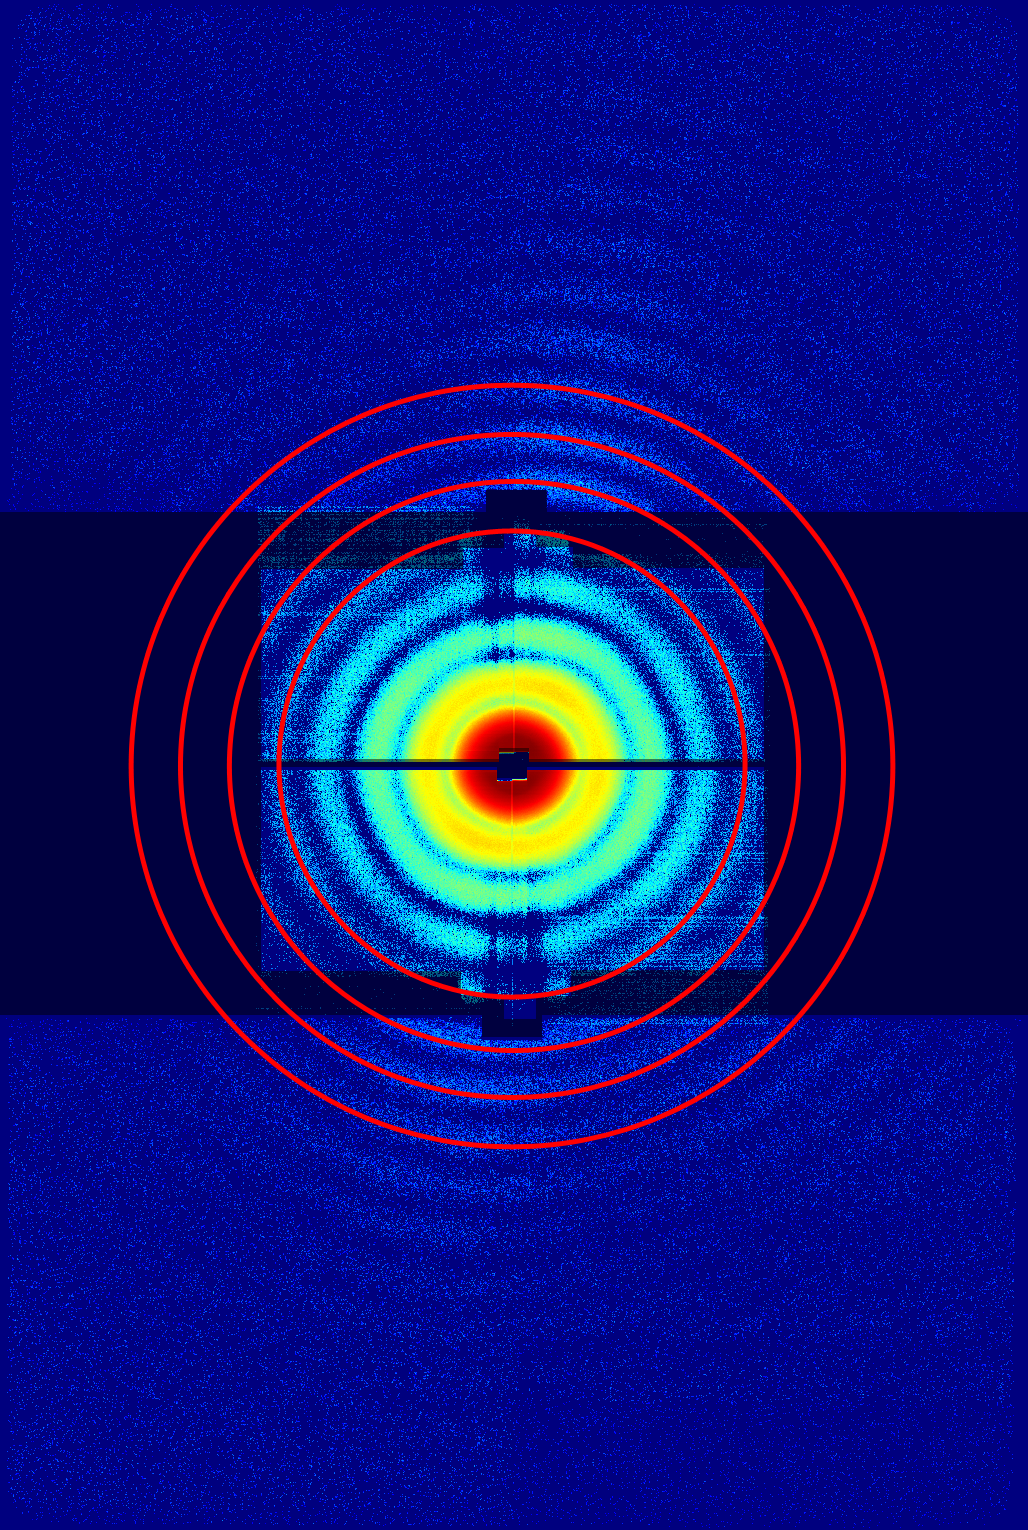
\includegraphics[width=0.80\textwidth]{images/pnCCD-image-geometry.png}
	\caption[Front and rear pnCCD arranged to combine measured diffraction image.]{A combined pnCCD image using the full image of the front pnCCD and a down-sampled image of the rear pnCCD. The red circles in the image are drawn in to visualize the alignment of the detectors. As described in the text, the intensities in the image are normalized and corrected for different electronic gains and distance to specific detectors. The shaded areas are not covered by the pnCCDs and are therefore masked out.}
	\label{fig:pnCCD-image-aligned}
\end{figure}
Figure \ref{fig:pnCCD-image-aligned}a shows a diffraction pattern from a spherical xenon cluster of $\sim 50$ nm in radius. The front pnCCD detector was set to slightly overlap with the rear pnCCD detector along the Y-axis but the front detector was set $\sim 365$ mm closer to the interaction region along the Z-axis. All four of LAMP's pnCCD modules have been combined in one image, and since the rear pnCCD is farther away from the interaction region it appears smaller on the combined image. The red circles are a help for the eye to align the modules and show how the diffraction pattern overlaps. In this case, the front pnCCD was operated in highest gain $\frac{1}{1}$ and the rear pnCCD was operated in lowest gain $\frac{1}{256}$.\\
\begin{figure}
	\centering
		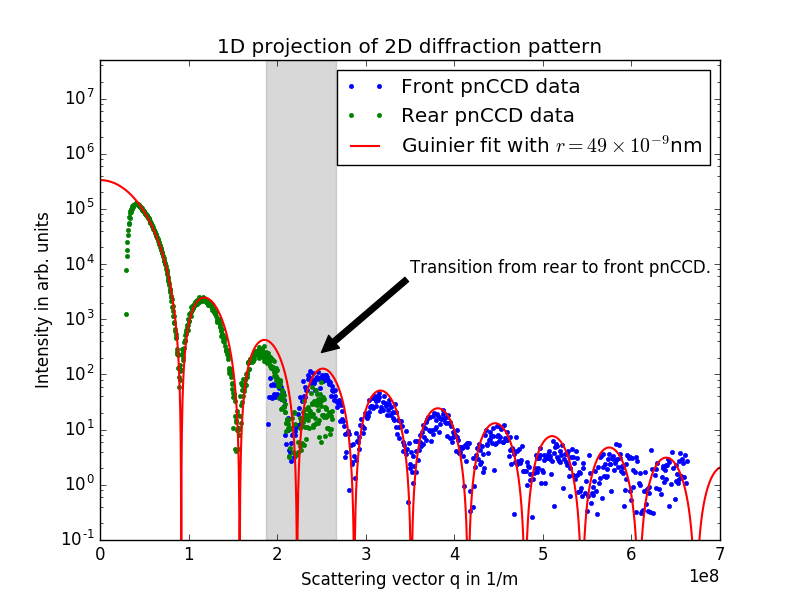
\includegraphics[height=0.50\textwidth]{images/pnCCD-1d-sum.png}
	\caption[Spherical projection of 2D diffraction image in 1D.]{In this graph a 2D diffraction image was projected onto 1D assuming a spherical symmetry of the diffraction pattern. The green data points are gathered from the rear pnCCD and the front pnCCD data points are reflected by the blue data points. The red curve is a simulated scattering curve from an ideal sphere that has a radius of $49 nm$. The amplitude of the red curve has been fitted to the data points and it agrees well with the data over 8 diffraction rings. The gray shaded area shows the transition area from rear to front detector.}
	\label{fig:pnCCD-1d-sum}
\end{figure}
The radial intensity profile yields valuable information about the geometric alignment and intensity normalization. Figure \ref{fig:pnCCD-1d-sum} shows the radial intensity profile of the spherical symmetric diffraction image over 5 orders of magnitude above the noise level. The red curve illustrates the expected scattering intensity of a spherical object with radius $49$ nm and the amplitude was fitted onto the rear pnCCD data. The curve showcases the validity of the detected signal up to the edges of the front pnCCD, where little signal is present. There are also some discrepancies from the red curve on the transition from the rear to front pnCCD, which are due to the shade projected from the front onto the rear pnCCD and the resulting lack of signal.
%
%
%
\subsection{Impact of X-ray pump -- X-ray probe on diffraction pattern}
\begin{figure}
	\centering
		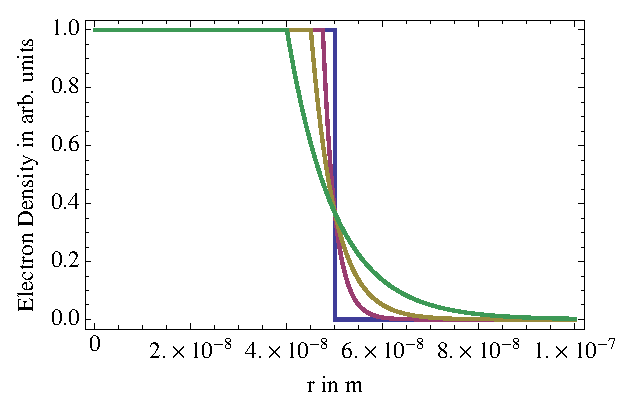
\includegraphics[width=0.49\textwidth]{images/electron-density-convoluted-object.eps}
		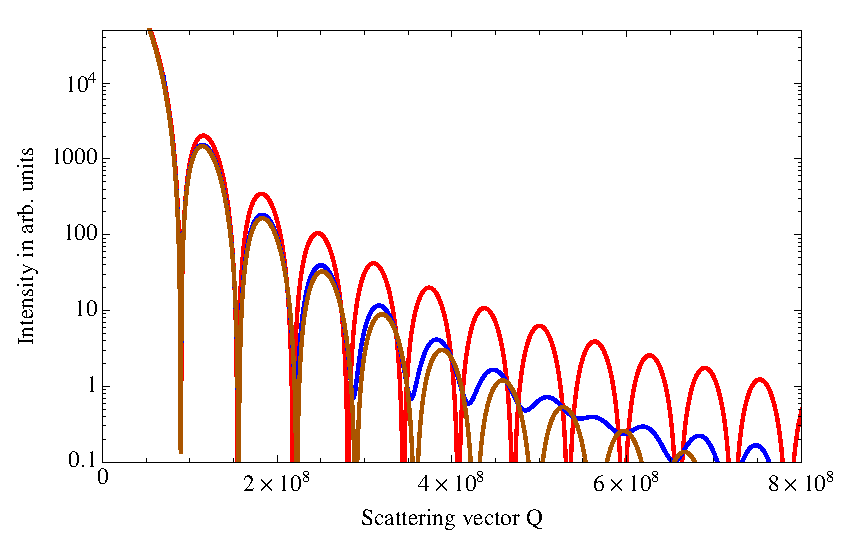
\includegraphics[width=0.49\textwidth]{images/beam-convoluted-with-object.eps}
	\caption[Influence of X-ray pump-- X-ray probe study in diffraction image.]{Left: electron density of an expanding spherical symmetric nanoplasma. Right: red line, scattering of an intact sphere. Brown, scattering of an expanding sphere with $k=5nm$. Blue, combined scattering of an intact and expanding sphere that has been pumped with $10\%$ and probed with $90\%$ of the overall pulse energy. See more information in text.}
	\label{fig:electron-density-convoluted-object}
\end{figure}
In a coherent diffractive imaging X-ray pump -- X-ray probe experiment, both pulses contribute to the scattering image. The pump pulse will project an image of the solid and intact cluster, while the probe pulse will propagate an image of the expanding, damaged cluster. In the present experiment, the pump pulse was set at $\sim10\%$ of the overall pulse energy, while the probe pulse was set to $\sim90\%$ of the overall pulse energy. In order to simulate the effects of the X-ray pump-- X-ray probe setup, a 1D simulation is conducted using electron densities $\rho\left(r\right)$ of spheres. Altough rare-gas cluster exhibit an icosahedral structure, at present resolution cluster can be well simulated using spheres. The spheres are allowed to expand after the model
\begin{align}
\rho\left(r, k\right)&=\begin{cases}
1& \text{for $R-k \geq r \geq 0$},\\
e^{\frac{(R-k)-r}{k}}&\text{for $R > r - k$},
\end{cases}
\intertext{with $R$ being the cluster radius and $k$ an expansion coefficient such that}
\int_{0}^{\infty}\rho\left(r, k\right)dr &= R,\quad \text{if } 0<k<R 
\label{eq:el-density-expanding}
\end{align}
The electron density can then be Fourier transformed into recipocal space using the transformation \citep{Guinier-1955-JWS}
\begin{equation}
F^{2}(Q)=A\left(\int_{0}^{\infty}\rho\left(r,k\right)\frac{\sin\left(Q r\right)}{Qr}4 \pi r^{2}dr\right)^{2},
\label{eq:guinier-fourier-transform}
\end{equation}
with $A$ being an intensity scaling factor. The electron densities for $R=50$ nm and $k=\{0,2.5,5,10\}$ nm are shown in figure \ref{fig:electron-density-convoluted-object} left. Figure \ref{fig:electron-density-convoluted-object} right showcases several cases of (expanding) spheres in reciprocal space. The red line is the scattering of a solid sphere $F_{\text{intact}}^{2}$, with $A$ being used to scale the intensity to typical experimental data. The brown curve is the scattering of an expanding sphere $F_{\text{expanding}}^{2}$ with $R=50$ nm and $k=5$ nm. Lastly, the blue curve corresponds to the case, where $A\cdot F^{2}\rightarrow A \cdot 10\% F_{\text{intact}}^{2}+A \cdot 90\% F_{\text{expanding}}^{2}$. Although the pump pulse influences the diffraction pattern visibly at high-Q values, the added signal remains in the noise level of $F^{2}(Q)<1$ (compare figure \ref{fig:pnCCD-1d-sum}).
%
%
%
\section{Phase retrieval from a single diffraction pattern}\label{sec:phase-retrieval}
%%%%%%%%%%%%%%
%- Short intro into phase retrieval
%%%%%%%%%%%%%%
As deducted in section \ref{sec:saxs}, coherent diffractive imaging merely measures the intensity in reciprocal space and the phase information, i.e. complex fields, are lost. Iterative algorithms can retrieve this lost information because there are only limited sets of phases that uniquely reproduce the diffraction image \citep{Bruck-1979-OpticsCom,Bates-1981-Optik}. To fully recover the original function, i.e. real and complex values of the diffraction pattern, the diffraction image must be oversampled\index{oversampling} \citep{Sayre-1952-ActCryst}. Here, the Nyquist-Shannon sampling\index{oversampling!Nyquist-Shannon sampling theorem} theorem says that a Fourier transformed object of size $X$ can be fully recovered if its sampling rate is at the Nyquist rate\index{oversampling!Nyquist rate} of $\frac{1}{2X}$\index{}. The Nyquist rate can be translated into a minimum (pnCCD) pixelsize in realspace using the following relation between a discrete Fourier transform and pixel length $\Delta_{r}$ \citep{Williams-2010-NJP}
\begin{equation}
\Delta_{r} = \frac{\lambda L}{2 X},
\label{eq:disc-fourier-relation-pixelsize}
\end{equation}
with the wavelength $\lambda$, the length to the detector $L$ and the object length along one dimension $X$. For typical experimental values, the sampling pixel size must be $\Delta_{r} \geq 2.7$ mm to fully recover the particle's (projected) electron density. In the present experiment, the pnCCD pixel size of $75 \times 75~\mu\text{m}^{2}$ samples the object sufficiently enough.
%
%
%
\subsection{Principle of phase retrieval}\label{sec:phase-retrieval-fundamental}
%%%%%%%%%%%%%%
%- Introduce some aspects from phase retrieval algorithms.
%%%%%%%%%%%%%%
\begin{figure}
	\centering
		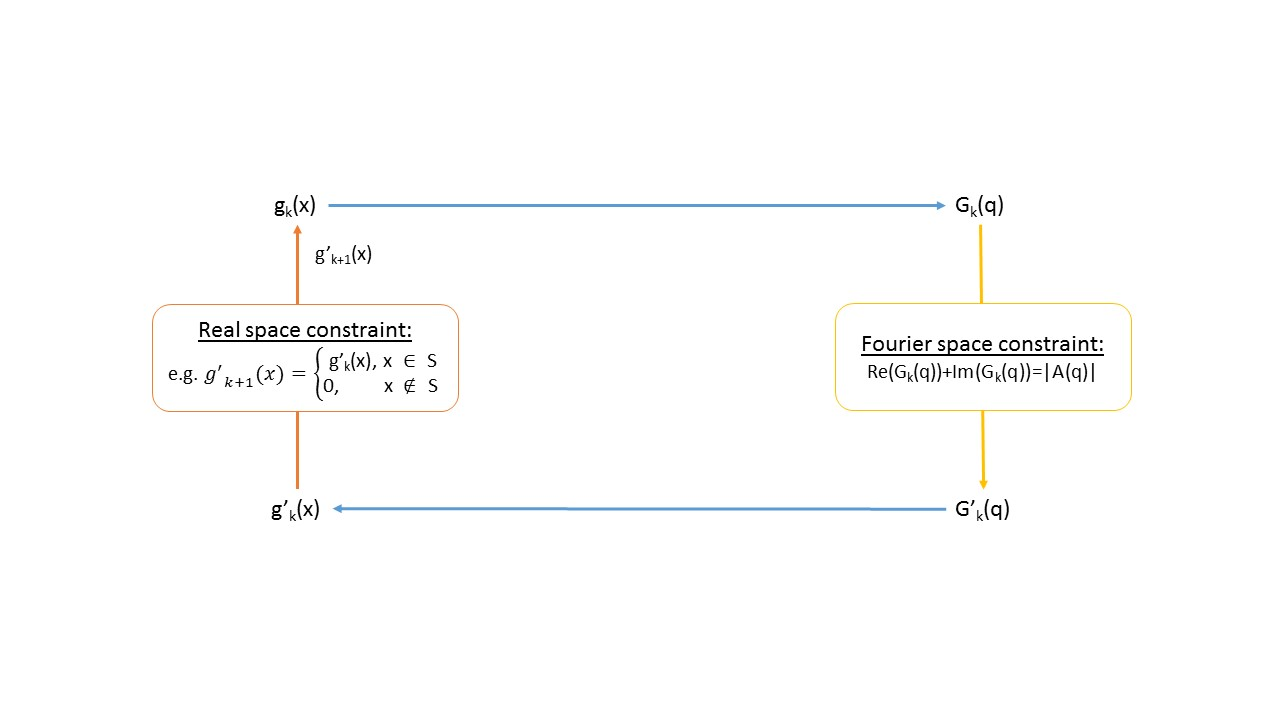
\includegraphics[width=0.80\textwidth]{images/phase-retrieval-algorithm.jpg}
	\caption[Example of a phase retrieval algorithm.]{Principle of a phase retrieval algorithm. The real space object $g_{k}\left(x\right)$ is Fourier transformed to $G_{k}\left(q\right)$. The function $G_{k}\left(q\right)$ is altered to fit the constraints set in Fourier space, hence $G'_{k}\left(q\right)$. $G'_{k}\left(q\right)$ is inverse Fourier transformed to $g'_{k}\left(x\right)$. After fulfilling the real space constraints the iterative starts again using $g_{k+1}\left(x\right)$. From \citep{Fienup-1982-AO}.}
	\label{fig:phase-retrieval-algorithm}
\end{figure}
To recover the phase from an oversampled diffraction pattern and thus reconstruct an image of the object, iterative algorithms have been developed \cite{Fienup-1982-AO}. Figure \ref{fig:phase-retrieval-algorithm} illustrates such an iterative algorithm, where the image of an object $g_{k}\left(x\right)$ is Fourier transformed to reciprocal space $G_{k}\left(x\right)$ and then back again resulting in $g_{k+1}(x)$, while sufficing certain constraints.\\
The constraints are rather strict defined in the reciprocal space as they have to reproduce the actual measurement $I=A\cdot A^{*}$, which is sometimes called the modulo constraint. The criteria that need to be met in real space can be chosen more freely. Generally, the recovered object should be physical, i.e. should be of a certain (known) size. One can introduce a support structure $S$ that meets the physical constraints and can therefore be used to, for example, zero outlying values. Throughout the iterations, the functions $g_{k}(x)$ evolve and eventually converge into a solution. If one uses the above criterion, one can show that the error between the reconstructions and the actual measurement continuously reduces, which is why it is commonly referred to as error-reduction algorithm \cite{Fienup-1978-OL}.
%
%
%
%
%\subsection{Solving the inverse problem}
\subsection{2D reconstructions and limitations}
%
%
%
\subsubsection{Hawk program for 2D image phase retrieval}
%%%%%%%%%%%%%%%%%
%- Describe Filipe's program
%%%%%%%%%%%%%%%%%
For all image reconstructions in 2D, the Hawk software package\index{Hawk software package} \citep{Maia-2010-JAC} has been used. Hawk is available under the GNU General Public License\footnote{Hawk copyright: \url{https://github.com/FXIhub/hawk/blob/master/Copyright}} and can be downloaded with installation instructions from \url{https://github.com/FXIhub/hawk}. In previous efforts to retrieve a real-space image from FEL based coherent diffractive imaging, Hawk has been used successfully in several reconstructions, ranging from viruses \citep{Seibert-2011-Nature,Ekeberg-2015-PRL} to other objects \citep{Seibert-2010-JPhysB}.
\begin{table}%[h!]
\centering
\begin{tabular}{ |c|c|}
 \hline
 \textbf{Parameter} & \textbf{Setting} \\ 
 %a & b & c & d & e \\
 %[0.5ex] 
 \hline
 Starting Guess & random phases \\ \hline
 Autocorrelation Selection & threshold \\ \hline
 Autocorrelaton Threshold & 0.04  \\ \hline
 Phasing method beta & 0.9  \\ \hline
 Beta range & 0 - $\infty$ \\ \hline
 Enforce positivity & false   \\ \hline
 Enforce real & false     \\\hline
Perturb weak reflections & false \\ \hline
Phasing algorithm & raar \\ \hline
Blur & 12 - 0.7 \\ \hline
Blur range & 0 - 12000 \\ \hline
Center image & false \\ \hline
Object area & 0.0022 - 0.0019 \\ \hline
Object area range & 0-8000\\ \hline
Support update algorithm & area \\ \hline
\end{tabular}
\caption{Typical parameter used in the Hawk software package.}
\label{tab:hawk-parameter}
\end{table}
The usage of the program is straight forward in three steps. First, the diffraction images are transformed into the '.cxi' format \citep{Maia-2012-NatMet}. Second, diffraction images are prepared in \textit{Hawk's editor}, where particular effort has to be made to create a proper mask. The mask  allows to forgo saturated, shadowed or otherwise faulty pixel. The software suite automatically interpolates between masked pixel. The successful edited '.cxi' file is then saved in Hawk's '.h5' format. Third, \textit{Hawk's phaser} can be used to iteratively retrieve the phase from the '.h5' intensity file. Typical parameter for the phaser can be found in table \ref{tab:hawk-parameter}. Here the \textit{RAAR algorithm} \cite{Luke-2005-IP} in combination with initially strong \textit{blurs}, extension of the \textit{phasing beta range} and a proper determination of the \textit{object area} (support structur) resulted in useful reconstructions. Note, that the \textit{object area} size differs from particle to particle, or intensity file to intensity file. After $10^{5}$ to $1.5\cdot 10^{5}$ iterations, the real space object typically converges.
%
%
%
\subsubsection{Resolution enhancement through combination of rear and front pnCCD}
%%%%%%%%%%%%%%%
%- Showcase difference of rear pnCCD only vs. front + rear pnCCD vs. front + rear pnCCD 'cropped' for best results. Recycle work from LAMP pnCCD paper
%%%%%%%%%%%%%%%
\begin{figure}
  \begin{center}
   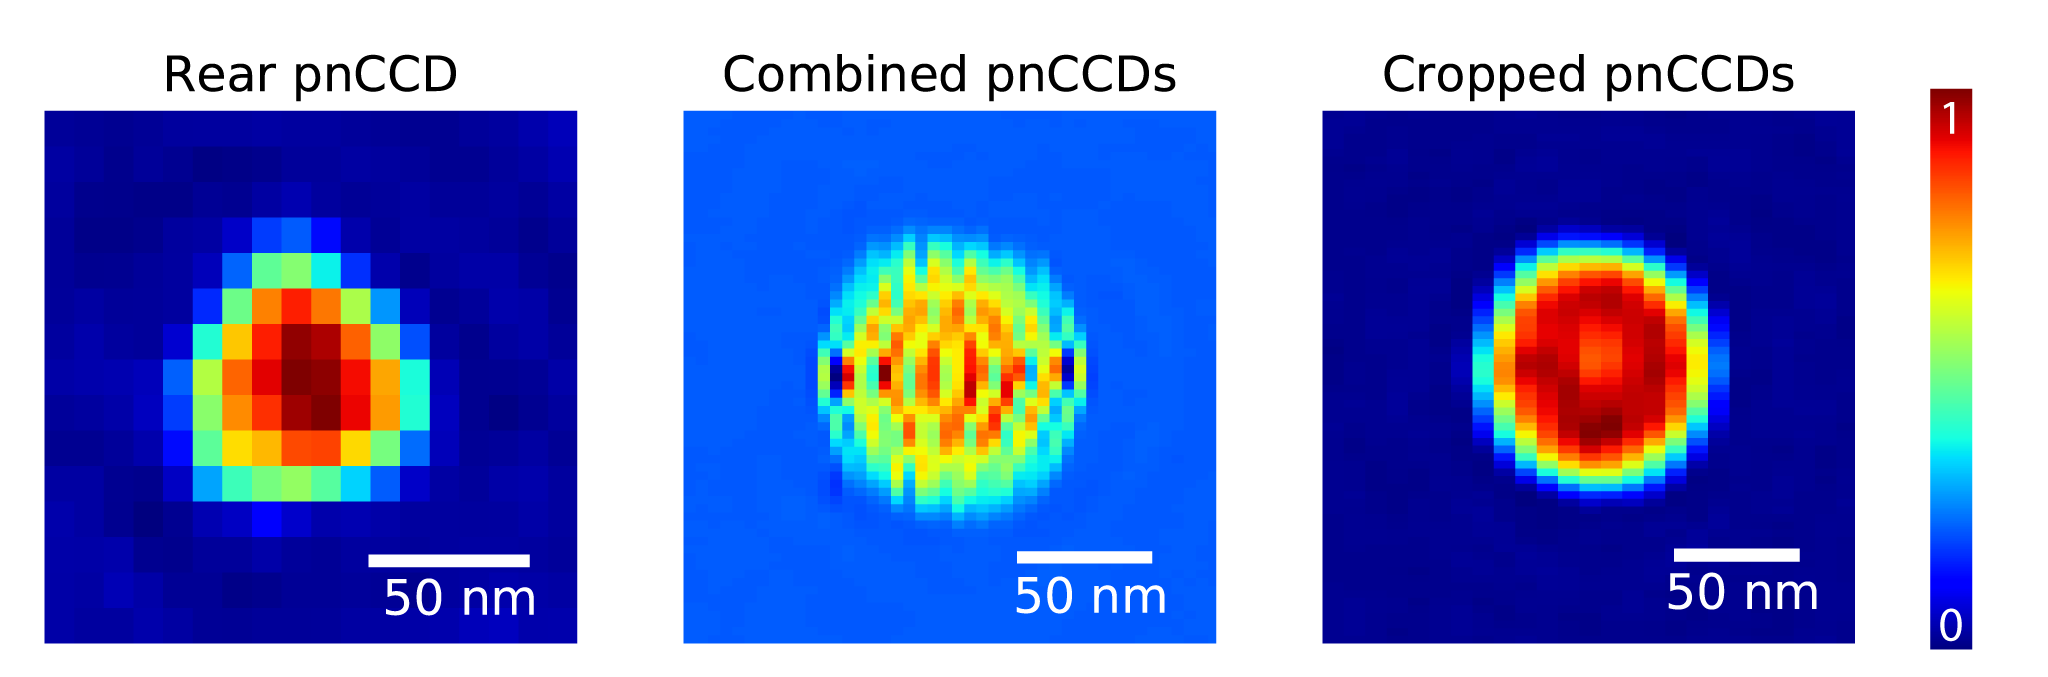
\includegraphics[width=0.8\linewidth]{images/Phase-retrieval-image.png}\\
   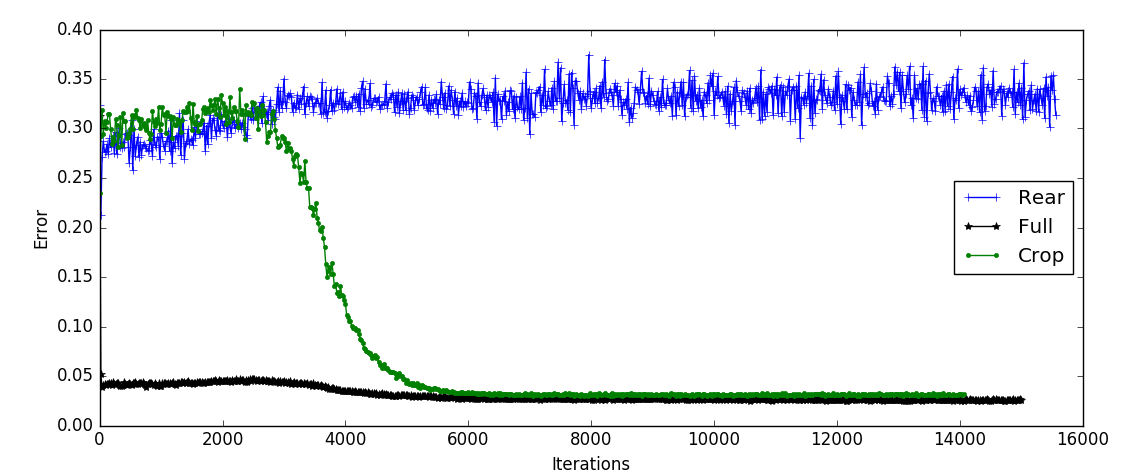
\includegraphics[height=3.5cm]{images/Phase-retrieval-error.png}
    \caption[Illustration of resolution enhancement and diffraction image cropping.]{A set of reconstructions of Xe-cluster yielded from the diffraction pattern in figure \ref{fig:pnCCD-image-aligned} and the corresponding real-space error over number of iterations. The real space image gathered from the rear pnCCD uses no data from the front pnCCD. This reconstruction shows a not spherical object although the density distribution appears to be reasonable for a nano-particle. The real space image reconstructed from the full front and rear pnCCD data set appears to be a spherical object but the missing areas disturb the diffraction pattern and it has become unphysical. The Xe-cluster reconstructed without the dead areas has the expected spherical shape and the density distribution appears to be physical.}
\label{fig:phase-retrieval-image}
  \end{center}
\end{figure}
While there is no consensus on how to define resolution in a coherent diffractive imaging pattern and the resulting reconstruction, there are various good estimates. A simple and conservative method to define resolution in a diffraction pattern is Abbe's criterion, which comes from microscopy and calculates the minimal resolvable feature size in a diffraction pattern. The fundamental limit that the minimal resolvable feature size is depended on the wavelength has also given us the inspiration to build short-wavelength machines such as the free electron laser and synchrotron light sources.\\
First, we can verify that we are in the far field by fulfilling the following requirement \cite{Williams-2010-NJP}
\begin{equation}
\frac{d^{2}}{\lambda L} \ll 1
\label{eq:far-field-test}
\end{equation}
with the wavelength of the X-rays $\lambda$, the distance to the detector $L$ and the object size $d$.\\
In the far field, Abbe's criterion can be written down as
% Internal note, Max did check that we are in the far field.
\begin{equation}
    d = \frac{\lambda}{2n \sin(\frac{\Theta}{2})},
\end{equation}
with the minimal resolvable feature size $d$, the refractive index $n$ and the half scattering angle $\frac{\Theta}{2}$. The scattering angle is restricted by either the active detector area, which goes back to the typical understanding of a numerical aperture, or the signal intensity up to certain angles. The latter is in interplay with the photon wavelength and object cross-sections. This interplay leads to the current assessment that very high energy photons, e.g. $8$ keV photons that are commonly used for crystallographic purposes, scatter too little signal. Additionally, low-$\vec{Q}$ scattering is often unresolvable due to straylight. As current results indicate, using $0.5-5$ keV photons ultimately leads to higher resolution images than using $8$ keV photons \citep{Aquila-2015-StrucDyn}.\\
In the far field, we can use the following equation to investigate the pixel size \cite{Williams-2010-NJP}
\begin{equation}
    \Delta_{s} = \frac{\lambda L}{N \Delta_{d}},
\label{eq:relation-pixel-fourier}
\end{equation}
with $L$ being the length from the interaction region to the detector, $\Delta_{i}$ being the linear pixel size that is linked to each other through the discrete Fourier transformation and $N$ being the side length of the discrete detector array.\\
Figure \ref{fig:phase-retrieval-image} top shows several reconstructions of xenon cluster at $\lambda = 1.0$ nm using different snippets of the diffraction pattern in figure \ref{fig:pnCCD-image-aligned}. If just the rear pnCCD is used for reconstructions, a maximum scattering angle of $\Theta\approx 4.2$° is recorded, which results in a minimal resolvable feature size of $d\approx 14$ nm. However, in the present data a shadow is cast on the CCD reducing the maximum scattering angle in the image \textbf{'Rear pnCCD'} to $\Theta\approx 3.8$° and thus the resolution to $d\approx 15$ nm. The pixel size is $\sim 10 \text{nm} \times \sim 12 \text{nm}$. The image \textbf{'Combined pnCCDs'} uses the whole data including the empty areas next to the rear pnCCD. The image shows an unphysical electron density distribution, which origins from the empty areas next to the rear pnCCD data. In these areas, the interpolation along the Y-axis/ extrapolation along the X-axis fails. The next image \textbf{'Cropped pnCCDs'} uses data in full extend along the Y-axis but crops the image along the X-axis such that the blank areas are excluded. The reconstruction converges into an object that appears physical. The maximum scattering angle here is $\Theta \approx 9.2$° and the resolution thus $d\approx 6$ nm. The pixel size here is $\sim 10 \text{nm} \times \sim 3 \text{nm}$.\\
This is a factor $\sim 5$ improvement over common cited studies in single particle imaging \citep{Seibert-2011-Nature} and still a factor $\sim 3$ better than \citep{Hantke-2014-NatPho}, where measured diffraction patterns have been 'computationally purified'. The resolution enhancement due to the combination of detectors can be abused further using EMC algorithms \citep{Loh-2009-PRE}, where multiple images can be arranged due to their rotation and averaged, hence filling the missing areas next to the rear pnCCDs and allowing 3D reconstructions with (few\footnote{Depending on the position of the front pnCCD.}) nanometer resolution.\\
%
%
%
\subsection{1D projections and phase reconstructions}\label{sec:1d-proj-and-phase-reconstruction}
%%%%%%%%%%%%%%%%
%- Describe my algorithm in 1D in detail
%%%%%%%%%%%%%%%%
To display many effects in diffraction pattern, they have sometimes been reduced from two dimensions to merely one. A 1D representation of the data allows easy to interpret comparison to analytical models. To reduce the 2D diffraction data to 1D the program shown in appendix \ref{sec:spherical-integration} has been employed. It is based on Matlab\index{Matlab} to efficiently iterate through pixel arrays. The input for this program are pedestal calibrated diffraction images that have unwanted areas masked out and a true image center defined. Key elements of the algorithm are to iterate through every pixel, filtering signal from noise, determining the $\vec{Q}$-value of every pixel and sum signal over $\vec{Q}$, while normalizing the data over pixel. Additionally, an algorithm has been designed to perform phase retrieval on the 1D data. This program is based on python and can also be found in appendix \ref{sec:1d-phase-retrieval-code}. The input for this algorithm are mirrored, zero-frequency (inverse) shifted 1D diffraction arrays. The algorithm follows the fundamental scheme described in sub-section \ref{sec:phase-retrieval-fundamental}. In the iterative algorithm, the realspace function is forced to be real and positive, which is also the error criterion in real space. The difference to the measured data yields the error criterion in Fourier space. The algorithm allows monitoring of the Fourier- and realspace error, the phase and the actual Fourier and realspace images. The iterative algorithm is aborted based on the error criterion.
%
%
%
\section{2D electron density and diffraction image simulations}\label{sec:2d-simulations}
%%%%%%%%%%%%%%%%%%%%%%%%%%%
% Describe 2D simulations
%%%%%%%%%%%%%%%%%%%%%%%%%%%
\begin{figure}
	\centering
		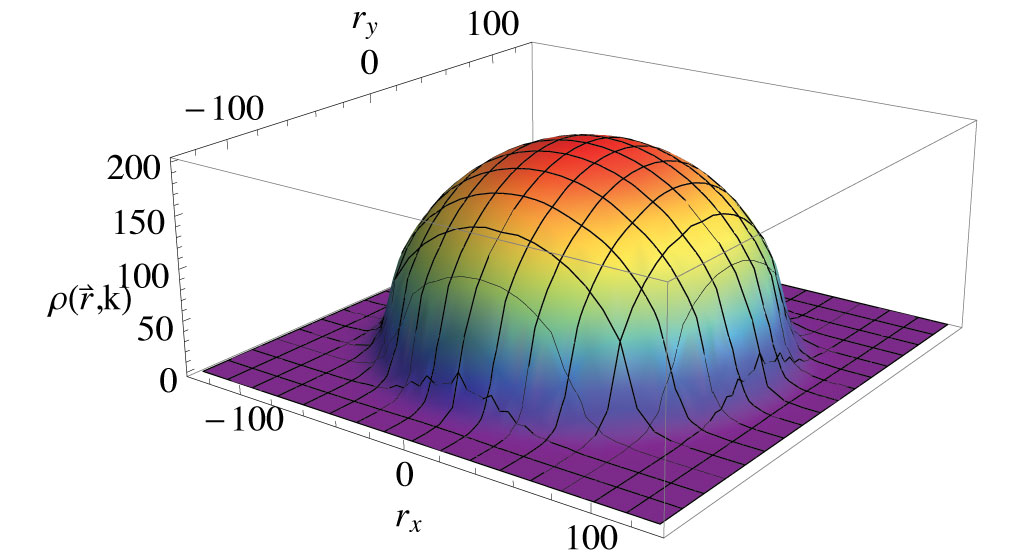
\includegraphics[width=0.49\textwidth]{images/cluster-generation-2D.eps}
		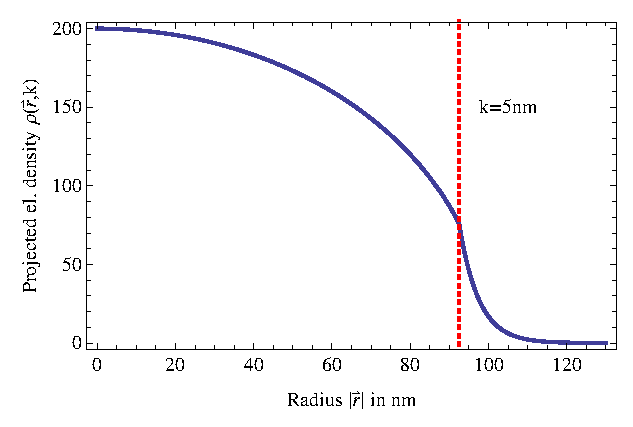
\includegraphics[width=0.49\textwidth]{images/cluster-generation-1D.eps}
	\caption[Used electron densities in 2D real and Fourier space simulations.]{Left: Electron density of a $R\approx 100nm$ expanding sphere with $k=5$ nm, projected onto a 2D plane. Right: Blue curve, spherical projection of the 2D projection to 1D. Red dashed line, point of expanding density at $k=5$ nm.}
	\label{fig:cluster-generation}
\end{figure}
The interpretation of the helium cluster doped with xenon data requires a more thorough investigation than with 1D fits possible. Therefore two dimensional studies were performed to simulate electron densities of (doped) clusters. The electron density is then Fourier transformed to yield 2D diffraction images, which can be compared to the experimental data. The 2D simulations can then optionally be reduced to 1D using a spherical integration (see subsection \ref{sec:1d-proj-and-phase-reconstruction}) to be easily compared to the experimental data and other analytical models. The clusters are approximated using spheres, which is at the current resolution an acceptable estimation of the icosahedral cluster structure. In the simulated cluster, i.e. core-shell system, the shell consists of one large cluster with low electron density (helium) and the core comprises smaller dense spheres (xenon) at different locations within the shell. Furthermore, the spheres can expand to simulate the effect of a nanoplasma expansion. We can express such spheres using the formalism
\begin{align}
\rho_{i}\left(\vec{r}, k\right)&=\begin{cases}
2 \sqrt{R^{2}-\left|\vec{r}\right|^{2}} \cdot \rho_{0}& \text{for $R-\frac{3 k}{2} \geq \left|\vec{r}\right| \geq 0$},\\
2 \sqrt{R^{2}-\left|\vec{r}\right|^{2}} \cdot \rho_{0} e^{\frac{(R-\frac{3k}{2})-\left|\vec{r}\right|}{k}}&\text{for $R > \left|\vec{r}\right| - \frac{3k}{2}$},
\end{cases}
\label{eq:el-density-expanding-2d}
\intertext{with $\rho_{0}$ being the density, $R$ being the cluster radius and $k$ an expansion coefficient such that}
\int_{0}^{\infty}\rho\left(\left|\vec{r}\right|, k\right)d\vec{r} &= R,\quad \text{if } 0<k<R 
\end{align}
Multiple spheres $\rho_{i}\left(\vec{r}\right)$, with $i=1,2,3,...$, can be positioned using $\vec{r}\rightarrow \vec{r}-\vec{r_{0}}$, with $\vec{r_{0}}$ being the center of mass of the sphere $\rho_{i}$. The density $\rho_{0}$ was set to $\rho_{0, \text{helium}}=1$ for liquid helium and $\rho_{0,\text{xenon}}=\frac{3.640}{0.1412}\approx 25.8$ for xenon. The numerator of the fraction for $\rho_{0,\text{xenon}}$ is the density of bulk xenon\index{Xenon!bulk density} in g/cm$^{3}$ and the denominator is the density for liquid helium\index{Helium!liquid density} in g/cm$^{3}$. Using equation \eqref{eq:el-density-expanding-2d}, a large array of $\sim 1500\times 1500$ is generated that is comparable to the combined pnCCD image array size. The array is then Fourier transformed\index{Fourier Transform} using Matlab's\index{Matlab} \textit{fft2} and the output is subsequently rearranged using \textit{fftshift}.\\
\begin{figure}
	\centering
		\includegraphics[width=0.80\textwidth]{images/cluster-sphere-intact.eps}
	\caption[Comparison of analytical derived scattering and numerical simulations.]{Comparison of analytical scattering from a sphere of radius $R=202$ nm (black curve), equation \ref{eq:scattering from sphere}, and scattering of a sphere of radius $R=202$ nm from 2D simulations projected onto 1D (green, dashed curve). Envelope of scattering intensity, called Porod's law, which is $\propto q^{-4}$ (red curve). The analytical scattering and developed simulations agree well with each other.}
	\label{fig:cluster-sphere-intact-2D}
\end{figure}
Figure \ref{fig:cluster-sphere-intact-2D} shows a comparison of the analytical derived scattering of a sphere (see equation \ref{eq:scattering from sphere}) with a radius of $r=202nm$ (black, dashed line) and the scattering of the 2D simulations reduced to 1D (green, solid line). The red curve is the envelope of the functions, called Porod's law that scales with $\propto q^{-4}$. The developed simulation agrees well with the analytical scattering.
%
%
%
\section{Acqiris data sampling}
%%%%%%%%%%%%%%%%%%%%%%%%%%%%%%
% Adjustments to iTOF data
% - Start value analysis
% - light peak jitter
%%%%%%%%%%%%%%%%%%%%%%%%%%%%%%
\begin{figure}
	\centering
		\includegraphics[width=0.49\textwidth]{images/Acqiris-waveform-readout.png}
		\includegraphics[width=0.49\textwidth]{images/firstDataPoint.eps}
	\caption[First data point in Acqiris sampling.]{Left image from \citep{Acqiris-manual}, it shows the schematics of the timing system in the Acqiris after receiving a trigger. Due to the finite sampling of the trace, the first data point can be before time zero. Right image is an histogram of the the timestamp from the first data point.}
	\label{fig:Acqiris-waveform-readout}
\end{figure}
An Acqiris digitizer (now called: Agilent U1065A) has been used to read out the waveform signal from the time-of-flight spectrometer. For technical reasons, the Acqiris sampling and the electronic trigger to start the readout process is generally not in sync. The electronic trigger can occur between sample $\{1,2,..,10\}$. In other words, the Acqiris reads out 40,000 samples but the trigger for the clock comes between sample 0 and 10. As it is illustrated in figure \ref{fig:Acqiris-waveform-readout} left, the time difference between the first data point and the time origin is within the sampling interval, thus $\{-1 \text{ns}, 0 \text{ns}\}$, at the sampling rate at 40,000, which is 1 ns per channel \citep{Acqiris-manual}. Figure \ref{fig:Acqiris-waveform-readout} right is an histogram of the First data point timestamp showing the evenly distributed discrepancy. As each read out sample would be different length $\{39991,39992,...,40000\}$, the LCLS DAQ group adds zeros to the end of each array to simplify the analysis of handling arrays of different lengths.\\
\begin{figure}
	\centering
		\includegraphics[width=1.00\textwidth]{images/TOF-trace-light-peak.eps}
	\caption[Using light peak to find absolute time zero in Acqiris traces.]{Top plot, average TOF trace of xenon cluster. Red curve, corrected run average to account for shifted light peak due to Acqiris sampling. Blue curve, uncorrected average. Bottom image, histogram of light peak channel position ranging between $\sim\pm 5$ of channel 1514.}
	\label{fig:TOF-trace-light-peak}
\end{figure}
However, in an LCLS experiment, the origin of time is best defined by the light peak. The time of flight spectrometer will detect photons scattered of the sample as the pulse is traversing through the system. Figure \ref{fig:TOF-trace-light-peak} bottom shows an analysis of the light peak channel position. The lightpeak occurs within a $\sim10$ ns window and is evenly distributed around channel 1514 due to the Acqiris sampling. Figure \ref{fig:TOF-trace-light-peak} top shows a merely averaged TOF trace (blue curve) and a TOF trace that has been corrected for the light peak occuring at different position (red curve). The LCLS DAQ changes the output of the Acqiris to start with time 0 or -1 and gives out a 40,000 channel long trace by adding zeros for every unsampled channel due to the trigger arrival.\\
The time-of-flight analysis in this thesis accounts for both of these effects and additionally corrects for a common baseline.
%
%
%
\section{Data filtering}\label{sec:hitfinding}
%%%%%%%%%%%%
%- Discuss the hitfinding.\\
%- iTOF vs. pnCCD\\
%- vs. Actual dynamics visible in diffraction images
%%%%%%%%%%%%
\begin{figure}
	\centering
		\includegraphics[width=0.49\textwidth]{images/filter-size.eps}
		\includegraphics[width=0.49\textwidth]{images/filter-sum-frontpnCCD.eps}
	\caption[Average cluster size correlated to measured intensity on front pnCCD.]{Left: Average Xenon cluster size of intense hits as a function of pump--probe delay $\Delta t$. Right: Average intensity on the front pnCCD of intense hits as a function of the pump--probe delay $\Delta t$.}
	\label{fig:filter-size-intensity}
\end{figure}
As described in the above sections, LCLS produces large amounts of data. This data has to be filtered to a point, where it can be used for phase retrieval. The coincident detection of diffraction image and time of flight spectroscopy allow great freedom to filter on useful events. For the present work, a useful event is the interaction of X-ray pump -- X-ray probe with a single cluster system. On the one hand, cluster produce the most intense signal on pnCCD and TOF detectors when they are in the center of the intensity profile of the LCLS beam \citep{Gorkhover-2012-PRL}. On the other hand, as the time delay $\Delta t$ of the X-ray pump -- X-ray probe is increased, the nanoplasma expansion leads to a decrease in signal on the pnCCD (see figure \ref{fig:filter-size-intensity}). This can be extrapolated to an extreme, where cluster would not produce any signal on the front pnCCD. In order to filter on the full bandwidth of interesting hits, a series of filters have been applied. Filtering on ion time of flight high charge states states has been successful in overall gathering images resolving pump--probe dynamics. In figure \ref{fig:filter-size-intensity} left, the xenon pump--probe data has been automatically pre-filtered on xenon ion high-charge states, leaving several thousand events that were then semi-automatically reduced to over 350 single-hit diffraction images. In this semi-automatic process it was determined, whether it was a single hit and the size of a cluster. The size determinations have been performed using the first maxima as described (see section \ref{sec:saxs}). The remaining events indicate a linear average cluster radius increase of $\sim15\%$ over the course of the first 800 fs at a given pump pulse energy. However, to perform phase retrieval and to solve the inverse problem, bright hits containing many photons are required. Therefore, an additional hitfinder on a snippet of the rear pnCCD detector has been implemented. This hitfinder determines the scattering intensity in single hits and brightest hits that show pump-probe dynamics have been selected undergo a phase retrieval to reveal their electron density. Events show dynamics, when the 1d reduction of the intensity profile differs from the scattering of an intact sphere, i.e. $F_{\text{intact}}^{2}/I >> 1$.
%
%
%
%\newpage
\chapter{Results and discussion}\label{ch:results}
%%%%%%%%%%%%%%%%
%- Introduction of what we are looking for, reminder of hypothesis
%%%%%%%%%%%%%%%%
Data from previous experiments \cite{Bostedt-2012-PRL,Gorkhover-2016-NatPho,Ferguson-2016-SciAdv}, where diffraction images and time-of-flight data were recorded in coincidence, show that the diffraction images carry transient information about the nanoplasma formation and expansion. The time-of-flight spectra contain valuable information about the atomic ionization as well as expansion dynamics from large ionized clusters and are therefore briefly discussed first in Section \ref{sec:itof-pump--probe}. The scattering response of the clusters to intense X-ray pulses is discussed in the following in Section \ref{sec:scattering-response}.\\[1\baselineskip]
%All data taken with coincident measurement of time-of-flight data and diffraction imaging in previous experiments  show that the diffraction images carry transient information of the nanoplasma formation and expansion during the pulse and are therefore the focus of the following discussion. However, the time-of-flight spectra contain valuable information about the atomic ionization as well as large ionized cluster expansion dynamics  This chapter is thus organized as follows: 
%
For the hasty reader the organization of the subsections may be helpful: Section \ref{sec:time-resolved-xe-atoms} discusses the time dependent response of Xe-atoms and -clusters to X-ray pump--X-ray probe beams in the ion TOF data. Section \ref{sec:hexe--and-he-TOF} continues the ion TOF data discussion on superfluid He- and mixed HeXe-clusters. Section \ref{sec:xenon-data} covers the scattering response of pristine Xe-clusters. Section \ref{sec:He-data-real} discusses the nanoplasma expansion of He-clusters in intense X-rays. Section \ref{sec:helium-data} addresses the agglomeration of heterogeneous HeXe-clusters and introduces the plum-pudding cluster model. Section \ref{sec:helium-xenon-data} discusses sample damage in HeXe-clusters using 2D-simulations. Section \ref{sec:comparison-of-He-and-HeXe-clusters} compares radiation damage of Xe-, He- and HeXe-clusters in intense X-rays to each other.\\[1\baselineskip]
%Section \ref{sec:itof-pump--probe} discusses the ion time-of-flight pump--probe data.
%First, the nanoplasma transition in pristine Xe-clusters is discussed in Section \ref{sec:xenon-data}. 
%The arrangement of Xe-atoms in HeXe-clusters is discussed in Section \ref{sec:helium-data} using 2D-simulations. Sample damage scenarios of HeXe-clusters are compared to simulations in Section \ref{sec:helium-xenon-data}. Section \ref{sec:comparison-of-He-and-HeXe-clusters} compares structural damage from the nanoplasma expansion for the different samples, He-, Xe-, and HeXe-clusters, to each other.\\[1\baselineskip]
%
The X-ray pulse parameters of this study are summarized in Table \ref{tab:beam-params} on Page \pageref{tab:beam-params}. It should be noted again that the split of the multipulse energy is \SI{10}{\percent} in the pump-pulse and \SI{90}{\percent} in the probe-pulse. This allows us to neglect the contributions of the pump-pulse to the scattering images (see Section \ref{sec:pump--probe-considerations}).
%The below discussed X-ray pump--X-ray probe data carries data from strictly speaking both pulses. Due to the split of the overall pulse energy in \SI{10}{\percent} to the pump-pulse and \SI{90}{\percent} to the probe-pulse, the contributions from the pump-pulse can be disregarded (see Section \ref{sec:pump--probe-considerations}).
%
%
%%%
\section{Ion time-of-flight X-ray pump--X-ray probe data}\label{sec:itof-pump--probe}
\subsection{Time-dependent response of Xe-atoms and -clusters to intense X-rays}\label{sec:time-resolved-xe-atoms}
%%%%%%%%%%%%%%%%%%%%%%%%%%%%%%%%%%%%%%%%%
%- Xe iToF dynamics\\
%- Slightly more of Xe higher charge-states present at longer delays.
%%%%%%%%%%%%%%%%%%%%%%%%%%%%%%%%%%%%%%%%%
\begin{figure}
	\centering
		\includegraphics[width=0.65\textwidth]{images/results/TOF-atomic-xenon2.png}
	\caption[Time-resolved answer of xenon atoms in TOF spectroscopy.]{Time-resolved answer of xenon atoms in TOF mass spectroscopy. The Xe-atom response to the X-ray pump--X-ray probe pulses from LCLS shows a resonant behavior in the high-charge states that peak at \SI{\sim250}{\femto\second} (see also Figure \ref{fig:TOF-atomic-xenon-time-dependent}).}
	\label{fig:TOF-traces-xenon-atoms}
\end{figure}
For the interpretation of the dynamic data from Xe- and HeXe-clusters it is first important to establish how individual atoms respond to a X-ray pump--X-ray probe experiment. Ion time-of-flight traces of atomic xenon at various time delays $\Delta t =$ \SIlist{0;120;250;400;800}{\femto\second} and X-ray pump-pulse only data are shown in Figure \ref{fig:TOF-traces-xenon-atoms}. All TOF traces below are averages of the \SI{\sim 10}{\percent} most intense hits of the respective run. The time-of-flight data indicate a resonant-like behavior in the time-domain as the atomic xenon high-charge states peak at $\Delta t\approx$ \SI{250}{\femto\second} with a clear increase. This is also shown in Figure \ref{fig:TOF-atomic-xenon-time-dependent}, where the total high-charge state ion-yield for Xe-atoms between the TOF range \SIrange{5.13}{6.50}{\micro\second} is plotted as a function of the time delay, $\Delta t$. The charge-state composition is highly dependent on the X-ray absorption process. For highly intense X-ray pulses, absorption is a complicated process involving multi-photon core-hole excitations and decay processes. Further theoretic investigations are needed to explain the spectra in more detail \cite{Ho-2014-PRL,Ho-2016-PC}. However, this resonant-like effect could be related to intensity-induced X-ray transparency \cite{Young-2010-Nature,Schorb-2012-PRL}. In this thesis experiment, the xenon 3d-subshell is efficiently photoionized by the X-ray pump-pulse. The resulting electron-holes in the 3d-subshell are typically repopulated on the few femtoseconds timescale due to the Auger decay, but the increasingly ionized atoms have also increasingly longer hole lifetimes, for example, previous studies show that $\text{Ne}^{8+}$ has core-hole lifetimes of \SI{\sim230}{\femto\second} \cite{Young-2010-Nature} making the atom increasingly transparent during the vacancy lifetime. In the present case, the absorption of photons from the probe-pulse is suppressed for delays $\Delta t \leq \SI{120}{\femto\second}$ because of this transparency. When the delay is $\Delta t = \SI{250}{\femto\second}$, the xenon 3d-subshell repopulates and the probe-pulse can efficiently photoionize the 3d-subshell again. But, why does the charge state distribution not level out for later delays $\Delta t >$ \SI{250}{\femto\second}? When the strongly pumped atom does not absorb energy near saturation, decay processes catch up and the nanoplasma dissipates energy in surrounding media. Subsequent recombination then could lead to less intense high-charge state populations.\\[1\baselineskip]
%
\begin{figure}
	\centering
	\includegraphics[width=0.6\textwidth]{images/results/atomic-charge-state-time-resolved.png}
	\caption[Time-dependent response of atomic xenon in TOF spectroscopy.]{The total of the high-charge state ion-yield for Xe-atoms between the TOF range \SIrange{5.13}{6.50}{\micro\second} or $(\sim \text{Xe}^{17+} \text{to } \text{Xe}^{10+})$ as a function of the time delay, $\Delta t$. The atomic Xe-ion TOF data show resonant behavior. As the time delay is varied in the range $\Delta t=$ \SIrange{0}{800}{\femto\second}, the high-charge states of atomic Xe-ions peak at \SI{\sim250}{\femto\second}.}
	%As the X-ray pump-pulse traverses through the xenon ions, the 3d-subshell becomes highly ionized and thus the atom becomes increasingly transparent for the probe-pulse ($\Delta t \approx$ \SIrange{0}{120}{\femto\second}). The electron-holes have a longer lifetime due to the highly ionized subshell. After the Auger decay populates the 3d-subshell, the atom becomes less transparent and the X-ray probe-pulse efficiently ionizes the atoms ($\Delta t \approx \SI{250}{\femto\second}$). Eventually, relaxation processes dissipate energy leading to fewer high-charge states ($\Delta t < \SI{400}{\femto\second}$).}
	\label{fig:TOF-atomic-xenon-time-dependent}
\end{figure}
%
%This makes the Xe-atoms become increasingly transparent 
%as the X-ray pulse propagates.
%The xenon high-charge states start low at $\Delta t = 0$ fs and then peak due to intensity-induced X-ray transparency \citep{Young-2010-Nature,Schorb-2012-PRL}. 
%In the present study, the xenon 3d-subshell is efficiently ionized by the X-ray pump-pulse. These electron-holes are typically repopulated on the few femtosecond timescale due to the Auger decay, however, the increasingly ionized atom has longer electron-hole lifetimes and the Xe-atoms become increasingly transparent as the X-ray pulse propagates. It has been measured that $\text{Ne}^{8+}$ has core-hole lifetimes of $~230$ fs. 
%
%
%
%The left panel of Figure \ref{fig:TOF-small-cluster-xenon} shows ion time-of-flight traces of small xenon cluster at different time delays $\Delta t =$ \SIlist{0;120;250;400;800}{\femto\second} and X-ray pump-only data. The xenon cluster in this data-set have an average radius of \SI{\sim 3.5}{\nano\meter}. The right panel of Figure \ref{fig:TOF-small-cluster-xenon} compares the total high-charge state ion yield for Xe-atoms and Xe-clusters and the dashed-lines are bspline fits to help the eye. For the \SI{\sim 3.5}{\nano\meter} radius Xe-cluster, the high-charge state time-dependence becomes increasingly complex. A theoretic study of these effects is beyond the focus of this work. However, the experimental data indicates that for shorter time delays, $\Delta t<$\SI{\sim 400}{\femto\second}, the time-dependency could be similar to the one of Xe-atoms. At longer time-delays, $\Delta t<$\SI{\sim 400}{\femto\second}, the high-charge state signal overall increases. This can be attributed to the expanding cluster and thus resulting lowering in Coulomb potential (see Figure \ref{fig:nano-plasma-schematic}) \cite{Krikunova-2009-NJP}. A further theoretic investigation that is beyond the scope of this thesis and typically requires access to supercomputers such as MIRA is needed and ongoing \cite{Ho-2016-PC}.\\[1\baselineskip]
%\begin{figure}
%	\centering
%		\includegraphics[width=0.49\textwidth]{images/results/clusterSummary_all}
%	\caption{caption}
%	\label{fig:TOF-regular-cluster-xenon}
%\end{figure}
The response of clusters to highly intense X-ray radiation is more complex. Size-dependent ionization \citep{Schorb-2012-PRL,Schutte-2015-JPhysB} and recombination in the nanoplasma \citep{Schutte-2014-PRL} alter the sample's ionization pathways. Ion time-of-flight traces of Xe-clusters are displayed in Figure \ref{fig:TOF-traces-xenon-cluster}. The time delay has been set to $\Delta t=$\SIlist{0;60;120;250;400;800} and also the pump only data is shown. The mean radius of the initially injected Xe-clusters are \SI{\sim 61}{\nano\meter} but they will expand by \SI{\sim20}{\percent} over a $\Delta t$ range of \SIrange{0}{800}{\femto\second} as discussed later in Section \ref{sec:xenon-data}. Unlike the atomic xenon data, the Xe-clusters show no clear resonant-like effect. The Xe-cluster data indicate a weak time-dependence of ionization and with increasing $\Delta t$, the high-charge states overall increase. This can be attributed to the expanding cluster. During the expansion, the cluster potential lowers \cite{Arbeiter-2011-NJP} and the electron transition dynamics become more complex \cite{Krikunova-2009-NJP}. To describe the time-dependent ionization of clusters in detail, a theoretic investigation that is beyond the scope of this thesis is needed and ongoing \cite{Ho-2016-PC}.
%owers the Coulomb potential (see Figure \ref{fig:nano-plasma-schematic}) and the more complex electron recombination possibilities \cite{Krikunova-2009-NJP}.
%For the \SI{\sim 61}{\nano\meter} radius Xe-cluster, the high-charge state time-dependence becomes increasingly complex. A theoretic study of these effects is beyond the focus of this work. However, the experimental data indicates that for shorter time delays, $\Delta t<$\SI{\sim 400}{\femto\second}, the time-dependency could be similar to the one of Xe-atoms. At longer time-delays, 
%The data show that the cluster type of signal is dominating the trace. At a time delay $\Delta t=800$ fs, the xenon high-charge states increase, while no other dynamic appears obvious from the average data. The larger cluster ensemble may undergo a similar resonant type behavior as atomic xenon, however, the large cluster ensemble seem to affect the ionization pathways and thus the timescale of the resonant type behavior.\\[1\baselineskip]
%
%Summarizing, atomic xenon, xenon cluster of mean radius $\sim XXX$ nm and Xe-cluster of average radius $\sim 61$ nm were investigated using an X-ray pump--X-ray probe setup coincidentally measuring spectroscopy and coherent diffractive imaging data. The ion spectroscopy data of atomic xenon high-charge states show a resonant type behavior as the time delay $\Delta t$ is varied from 0 fs to 800 fs. The effect peaks, i.e. is resonant around 250 fs. Small xenon cluster exhibit a similar behavior as atomic signal because atomic signal is dominating the high-charge states. The signal from larger xenon cluster of radii $\sim 61$ nm is dominated by xenon charge fragments. An increase in the xenon high-charge states is observed at 800 fs, allowing us to conclude that the ionization dynamics have changed. It is interesting to note that altough larger cluster absorb overall more energy, the ensemble of atoms that is bound in the cluster is able to collectively change, here slow, ionization pathways. This behavior may be reproduced in other nano-samples such as bio-molecules or artifical tamper layers.
\begin{figure}
	\centering
		\includegraphics[width=0.65\textwidth]{images/results/TOF-regular-cluster-xenon2.png}
	\caption[Time-resolved answer of xenon clusters in TOF spectroscopy.]{Time-resolved answer of xenon clusters in TOF mass spectroscopy. Unlike the atomic response, Xe-clusters show no clear resonance and overall have a weak time dependence.}
	\label{fig:TOF-traces-xenon-cluster}
\end{figure}
%
%
%
%%%%%%%%%%%%%%%%%%%%%%%%%%%%%%%%%%%%%%%%
\subsection[Time-resolved response of highly ionized He- and HeXe-clusters]{Time-resolved response of He- and HeXe-clusters in intense X-rays}\label{sec:hexe--and-he-TOF}
%%%%%%%%%%%%%%%%%%%%%%%%%%%%%
% - Subsection for iToF data, important to compare to HeXe data.
%%%%%%%%%%%%%%%%%%%%%%%%%%%%%
\begin{figure}
	\centering
		\includegraphics[width=0.65\textwidth]{images/results/TOF-helium-cluster2.png}
	\caption[Time-resolved answer of He-clusters in TOF spectroscopy.]{Ion time-of-flight traces of He-cluster with a radius of $r_{\text{He}}\approx \SI{810}{\nano\meter}$. Although minor changes in the charge fragmentation are observed, we shall note that there are no He$^{2+}$ ions in this data. The absorption cross-section of helium are too low to lead to doubly-charged states \citep{Ho-2016-PC}.}
	\label{fig:TOF-helium-cluster}
\end{figure}
%
He-droplets exhibit a weak response to the X-ray pump--X-ray probe delay similar to the Xe-cluster. Figure \ref{fig:TOF-helium-cluster} shows ion time-of-flight data of pristine He-cluster at pump--probe delays $\Delta t=$ \SIlist{0;250;800}{\femto\second}. The pristine He-droplets have an average radius of $r_{\text{He}}\approx$ \SI{810}{\nano\meter} that has been derived from the cluster growth scaling laws (see Section \ref{sec:homogenous-cluster}). The data show an overall similar behavior regardless of the delay $\Delta t$, although minor changes in the charge fragmentation distribution can be seen. The He-data is shown for comparison to the HeXe-cluster data presented below. For the comparison, it is important to note that the TOF traces indicate no contribution of doubly-charged helium atoms. The lack of double-charged helium can be explained by the comparably low absorption cross-sections of helium (see Table \ref{tab:helium-xenon-ionization}) \cite{Ho-2016-PC}.\\[1\baselineskip]
%
\begin{figure}
	\centering
		\includegraphics[width=0.65\textwidth]{images/results/TOF-helium-xenon-cluster-60-2.png}
	\caption[TOF spectra of HeXe-clusters with a \SI{\sim 0.6}{\percent} Xe-doping at various $\Delta t$.]{Ion TOF spectra of HeXe-cluster with radius $r\approx$ \SI{600}{\nano\meter} and a Xe-doping level of \SI{\sim 0.6}{\percent}. Only neglible contributions from Xe-charge-fragments are observed. Conversely, doubly-charged He$^{2+}$-ions are detected and the kinetic energy release of the He-peaks varies. With increasing delay time, the He-ions reveal a time-dependence.}
	\label{fig:TOF-helium-xenon-cluster-60}
\end{figure}
%
Next, HeXe-cluster with a radius of $r_{\text{He}}\approx$ \SI{600}{\nano\meter} and a \SI{\sim 0.6}{\percent} doping level of xenon are discussed. For clarity, this is measured through the helium depletion measurement, which was discussed in Section \ref{sec:heterogeneous-cluster}. At this doping level, the helium depletion is \SI{\sim 62}{\percent}. The TOF spectra are shown in Figure \ref{fig:TOF-helium-xenon-cluster-60} for the delays, $\Delta t=$ \SIlist{0;200;800}{\femto\second}. Most notable is the presence of $\text{He}^{2+}$ ions and the strongly increased signal from $\text{He}^{+}$ ions. But, only few xenon charge fragments are observed. This is counter-intuitive as the absorption cross-section from xenon is much larger than from helium (see Table \ref{tab:helium-xenon-ionization}). We can therefore hypothesize that ultrafast charge-transfer occurs between the Xe-particles and the He-droplets \cite{Hoener-2008-JPB}. The He-droplet functions as electron reservoir for the Xe-clusters and therefore they can recombine. The neutral Xe-particles are not detected by the ion TOF spectrometer and barely any signal of Xe charge fragments is detected \cite{Hoener-2008-JPB,Hau-Riege-2007-PRL}. The absence of Xe charge fragments indicates also the sample integrity of the Xe-particles. As we look at the longer delays $\Delta t$, it is interesting that the He-ion signals of the HeXe-clusters show a strong time-dependence. Similar to the atomic xenon data, we observe that the He-ion signal shows a resonant-type behavior and at $\Delta t =$ \SI{200}{\femto\second}, the signals from $\text{He}^{2+}$ and $\text{He}^{+}$ peak. We can make use of the earlier discussion around the data shown in Figure \ref{fig:TOF-atomic-xenon-time-dependent} and \ref{fig:TOF-helium-cluster} and conclude that this resonant-like behavior does not originate from the absorption and ionization dynamics of the He-droplet but rather from the Xe-atoms with which the He-droplet is doped. This allows us to hypothesize that there must be an ultrafast kinetic energy transfer process as charge-transfer alone does not explain the increase in kinetic energy of the He-ions \cite{Hoener-2008-JPB,Sugishima-2012-PRA,Muller-2015-JPhysB}. For example, collisions could transfer energy from the Xe-particles to the He-droplet. This thought can be expanded and it is theoretically predicted that electron-electron collisions of trapped electrons in the cluster potential occur frequently \cite{Arbeiter-2011-NJP}. These collisions could be responsible for this energy exchange. This indication of trapped electrons is interesting because these electrons damage the sample due to secondary collisional ionization \cite{Hau-Riege-2004-PRE} and we will discuss some implications for diffractive imaging below. Note that the He-dimer signal decreases steadily, which can be attributed to the nanoplasma formation. The weakly bound He-dimer bonds will break as a result of the ionization and increased kinetic energy, such that they contribute, for example, as He$^{+}$-ions to the TOF data.\\[1\baselineskip]
%e.g., collisional energy transfer from the Xe-particles to the He-droplet
%
%Comparing the data from Figure \ref{fig:TOF-helium-cluster} and \ref{fig:TOF-helium-xenon-cluster-60} allows us to conclude that xenon cluster transfer energy to the helium cluster that they are embedded in. This process is very efficient since the resonant behavior that origins from the xenon atoms is constituted in the helium signal, while the xenon signal steadily decreases. Therefore,  This behavior is similar to \citep{Hoener-2008-JPB} but differs in it's geometric arrangement.\\
%
\begin{figure}
 	\centering
 		\includegraphics[width=0.65\textwidth]{images/results/TOF-helium-xenon-cluster-13-2.png}
 	\caption[TOF spectra of HeXe-clusters with \SI{\sim 0.06}{\percent} Xe-doping at various delays.]{Ion TOF spectra of HeXe-cluster with radius $r\approx$ \SI{775}{\nano\meter} and a \SI{\sim 0.06}{\percent} xenon doping level. These weaker doped HeXe-clusters show a lower He$^{2+}$-ion count and kinetic energy release. Barely any Xe-ions are detected.}
 	\label{fig:TOF-helium-xenon-cluster-13}
\end{figure}
%
If the He-ion composition is strongly driven by the doped Xe-atoms, one would expect a dependence on the Xe doping-level. Therefore, He-droplets with a radius of $r\approx$ \SI{775}{\nano\meter} and a \SI{\sim 0.06}{\percent} doping are discussed next. This is a \num{\sim 10} times less doping than the above discussed data and the He$^{2+}$-ion signal should therefore be less intense and broad to support the hypothesis. For completeness, the helium depletion is \SI{\sim 13}{\percent}. Figure \ref{fig:TOF-helium-xenon-cluster-13} shows the ion TOF data at delays $\Delta t=$ \SIlist{0;800}{\femto\second}. We note, again, the presence of $\text{He}^{2+}$ ions and an increased signal from $\text{He}^{+}$ ions. Although the He-droplet is larger, the $\text{He}^{2+}$-ion peak is clearly less intense and less broad than the above data with stronger Xe-doping. Xe-ions are barely detected. These data support the hypothesis that the Xe-particles drive the He-ionization through the above discussed processes. The detection of the initially photoionized xenon is more suppressed than in the above data through recombination effects and a larger electron reservoir. By varying the time delays $\Delta t$, the height of each He-ion peak shifts and a time-dependence is clearly visible. The $\text{He}^{2+}$ and $\text{He}^{+}$ states become less intense, but a stark increase in $\text{He}_{2}^{+}$ and $\text{He}_{3}^{+}$ peaks is observed. This could be a sign of a less violent nanoplasma expansion, where charge fragments not fully disintegrate into their atomic components, i.e., $\text{He}^{2+}$-ions, than in the above strongly doped data.\\[1\baselineskip]
%
%Summarizing, we studied the idea that a low-Z material acts as a sacrificial layer for the high-Z material using TOF mass spectroscopy. 
In summary, pristine He-droplets show little time-dependence as $\Delta t$ is varied and mostly singly-charged $\text{He}^{+}$- and $\text{He}_{2}^{+}$-ions are measured. If the He-droplets are doped with xenon, doubly-charged $\text{He}^{2+}$-ions are detected, the kinetic energy release is stronger, and the time-of-flight data reveal a He-ion time-dependence that is comparable to the one of Xe-atoms. As the Xe-doping is decreased, the presence of $\text{He}^{2+}$ ions becomes less frequent. This HeXe-cluster data indicates that the ionization dynamics of the He-ions are driven by the encapsulated Xe-atoms. A charge transfer from the initially photoionized Xe-atoms to the He-droplet is likely the dominating process leading to these TOF traces. This has also been shown previously theoretically \cite{Hau-Riege-2007-PRL} and in static studies \cite{Hoener-2008-JPB,Sugishima-2012-PRA,Muller-2015-JPhysB}. If the HeXe-cluster TOF data is compared to the pristine Xe-cluster TOF data, it becomes obvious that the Xe-particles preserve their integrity better when they are encapsulated in a He-cluster \cite{Hoener-2008-JPB,Muller-2015-JPhysB,Sugishima-2012-PRA}.
%This data could originate from an ultrafast and efficient kinetic energy transfer from the Xe-particles to the He-droplet. Collisions could drive this energy transfer. Charge-transfer ionization could drives the He-ion composition. Thereby, the He-droplet acts as an electron reservoir and the initially photoionized Xe-atoms recombine efficiently. Neutral xenon is not detected by the TOF mass spectrometer and this indicates that the Xe-particles in the HeXe-clusters preserve their integrity much better than pristine Xe-clusters. Pristine Xe-clusters are efficiently ionized and Xe-charge-fragments of Xe$^{25+}$ are observed, which indicate that the pristine Xe-cluster exhibit violent sample damage. Similar results have also been studied in \citep{Hoener-2008-JPB,Mikaberidze-2008-PRA}.
%
%
%
%%%%%%%%%%%%%%%%%%%%%%%%%%%%%%%%%%%%
%%%%%%%%%%%%%%%%%%%%%%%%%%%%%%%%%%%
%%%%%%%%%%%%%%%%%%%%%%%%%%%%%%%%%%%%
\section{Scattering response of rare-gas clusters}\label{sec:scattering-response}
%
%This section discusses the diffraction images that were obtained in the X-ray pump--X-ray probe study. The discussion begins with an assessment of the X-ray induced radiation damage of pristine Xe-clusters, whereby first diffraction images and then reconstructions are discussed, and an analysis of diffraction images of pristine He-droplets. This is followed by the discussion of the shape of HeXe-clusters. The section ends by discussing and comparing X-ray induced damage in HeXe-clusters to Xe- and He-clusters.
%
%
%
\subsection{Structural damage in Xe-clusters induced by intense X-rays}\label{sec:xenon-data}
%%%%%%%%%%%%%%%%%%%%%%%%%%%
%- Presentation of Xe data
%%%%%%%%%%%%%%%%%%%%%%%%%%%
% INTRO
XFELs can create high-quality diffraction images from single particles. All diffraction images carry transient information of the sample during the pulse \cite{Bostedt-2012-PRL}. In a pump-probe experiment, time-resolved structural information can be extracted from the diffraction images, such as the surface softening of the nanoplasma \cite{Gorkhover-2016-NatPho}. This thesis experiment follows the X-ray induced nanoplasma expansion up to \SI{800}{\femto\second} for the first time.
%A very distinct time-resolved signal originates from the surface softening of the clusters as they undergo the nanoplasma expansion \cite{Gorkhover-2016-NatPho}. To investigate this time-dependent signal, 
To start out, \numrange{30}{60} diffraction images per delay step from Xe-clusters are analyzed (see Section \ref{sec:hitfinding}) and their radius is determined. This leads to a high-throughput evaluation of several hundred clusters, whereby Equation \eqref{eq:scattering from sphere} is exploited to automatically fit diffraction images.\\[1\baselineskip]
% SIZE EFFECTS
\begin{figure}
	\centering
		\includegraphics[width=0.70\textwidth]{images/results/size-distributions.png}
	\caption[Single Xe-cluster size distribution at varying time delay $\Delta t$.]{Size evaluation of \num{\sim 30} single Xe-cluster hits per time delay $\Delta t$ step. At $\Delta t=\SI{0}{\femto\second}$, the size distribution follows in approximation an expected log-normal distribution. At $\Delta t=\SI{800}{\femto\second}$ the distribution broadens and shifts towards larger radii due to the nanoplasma transition.}
	\label{fig:size-distributions}
\end{figure}
Supersonic gas jets always produce a distribution of cluster sizes (see Section \ref{sec:homogenous-cluster}). Such a distribution of cluster radii is shown in Figure \ref{fig:size-distributions} for the X-ray pump--X-ray probe time delays, $\Delta t =$ \SIlist{0;800}{\femto\second}. The size distribution of Xe-clusters follows a log-normal distribution \citep{Schutte-2002-IJMS} and for $\Delta t=0$ fs, the mean cluster radius is \SI{61}{\nano\meter}. When the imaging pulse is delayed by $\Delta t=$ \SI{800}{\femto\second}, the mean cluster-radius increases to \SI{74}{\nano\meter} and the size-distribution becomes broad. This can be clearly attributed to the nanoplasma expansion. The Xe-cluster size distribution may become more broad due to a distribution of the pump-pulse power density. Shot-to-shot fluctuations result in different nanoplasma expansion speeds, $v_{\text{exp}}$, as discussed below.\\[1\baselineskip]
%
\begin{figure}
	\centering
		\includegraphics[width=0.49\textwidth]{images/results/filter-size.png}
		\includegraphics[width=0.50\textwidth]{images/results/filter-sum-frontpnCCD.png}
	\caption[Average cluster size correlated to measured intensity on front pnCCD.]{Average xenon cluster size of intense hits as a function of pump--probe delay $\Delta t$ (left panel). Average intensity on the front pnCCD of intense single-shot hits from single Xe-cluster as a function of the pump--probe delay $\Delta t$ (right panel).}
	\label{fig:filter-size-intensity}
\end{figure}
%
A summary of the of the Xe-cluster radii increase over several pump--probe delay steps can be found in Figure \ref{fig:filter-size-intensity}. The mean radii and standard deviations of the log-normal distributions are plotted for $\Delta t=$ \SIlist{0;120;250;400;800}{\femto\second} and fitted linearly. These data suggest that the nanoplasma expansion speed, $v_{\text{exp}}$, is rather constant over the observation window. Theoretical studies of nanoparticles \cite{Hau-Riege-2004-PRE,Mikaberidze-2008-PRA,Ho-2016-PRA} predict that the expansion speed indeed becomes constant after a few ten femtoseconds, which the system needs to thermalize. We can determine the expansion speed using the mean increase of cluster-radii over $\Delta t=$ \SIlist{0;800}{\femto\second} and note $v_{\text{exp}}\approx \SI{15250}{\meter\per\second}$. This indicates that Xe-nanoparticles that are irradiated with typical LCLS pulses undergo a violent and rapid explosion.\\[1\baselineskip]
%
We can use the expansion speed to estimate the electron temperature of the nanoplasma, as it has been done similarly before \cite{Gorkhover-2012-PRL}. Thereby, we should note that the electron gas of the nanoplasma thermalizes with the ions on the few femtoseconds time-scale and follows a Maxwell-Boltzmann distribution \cite{Arbeiter-2011-NJP}. If we now find a temperature for the Maxwell-Boltzmann distribution that has the expansion speed, $v_{\text{exp}}$, as mean velocity, we can estimate the electron temperature to be \SI{\sim 125}{\electronvolt}. This compares to temperatures that can be found inside the sun.\\[1\baselineskip]
%
We can also compare the electron temperature to a similar NIR pump--X-ray probe nanoplasma study on Xe-clusters \cite{Gorkhover-2016-NatPho}, where electron temperatures of \SI{\sim 200}{\electronvolt} have been found. The difference in electron temperature and expansion speed is attributed to the difference between the NIR and X-ray pump-pulse parameters and the corresponding absorption cross-sections. The NIR pump-pulse has a wavelength of \SI{800}{\nano\meter}, a focal spot size of \SI{1600}{\micro\meter\squared}, and power densities of \SI{\sim e15}{\watt\per\square\centi\meter} \cite{Gorkhover-2016-NatPho}. The X-ray pump-pulse in this study has a wavelength of \SI{1.5}{\nano\meter} and power densities of \SI{\sim 2e16}{\watt\per\square\centi\meter}. The NIR strong-field absorption cross-section of a xenon atom can be estimated to be \SI{\sim 30}{\mega\barn} using the above power densities (from Reference \cite[][1826]{Fennel-2010-RMP}), and the X-ray absorption cross-section for atomic xenon is \SI{\sim 3}{\mega\barn} (from Figure \ref{fig:photoionization}). Let us perform a very simplified cross-section estimation similar to Equation \eqref{eq:absorption-cross-section} using \SI{25}{\nano\meter} radius Xe-clusters. Given the above parameters, this estimation indicates that a Xe-cluster would absorb \SI{\sim 93}{\kilo\electronvolt} in the NIR and \SI{\sim 79}{\kilo\electronvolt} in the X-ray wavelength region. The relative absorbed energy in X-ray versus NIR is $\tfrac{79}{93}\si[per-mode = fraction]{\cancel\kilo\electronvolt\per\cancel\kilo\electronvolt}\approx\SI{85}{\percent}$. This relative difference can be compared to the relative difference in electron temperatures of the X-ray-- vs. the NIR--study, which is $\tfrac{125}{200}\si[per-mode = fraction]{\cancel\electronvolt\per\cancel\electronvolt}\approx\SI{63}{\percent}$. Given this estimate, it is clear why the electron temperature in the NIR study is higher than in the here presented X-ray study. It is noted that, for example, transient scattering factors and cluster cooling processes \cite{Fennel-2010-RMP} do play a significant role in this absorption process, which do vary the actual absorbed energies drastically \cite{Fennel-2010-RMP} and are disregarded in this simplified estimate.\\[1\baselineskip]
%X-ray absorption cross-section of xenon, $\sigma_{\text{X-ray}}=\SI{\sim 3}{\mega\barn}$ is much smaller than the IR cross-section, $\sigma_{\text{IR}}=\SI{\sim 30}{\mega\barn}$. Ultimately, the Xe-clusters absorb more energy from IR pump-pulses than X-ray pump-pulses of similar power density.\\[1\baselineskip]
% NO OF SCATTERER
\begin{figure}
	\centering
		\includegraphics[width=0.80\textwidth]{images/results/number-of-scatterers.png}
	\caption[Time-resolved behavior of number of scatterers due to nanoplasma expansion]{Scattered intensity $I_{0}$ in arb. units at $\vec{Q}\rightarrow 0$ of Xe-clusters. This is proportional to the total number of scatterers squared, $N_{e}^{2}$. The red curve is a guide for the eye (see Section \ref{sec:xenon-data}).}
	\label{fig:number-of-scatterer}
\end{figure}
%
Let us continue by looking at the time-dependent behavior of electrons. During the pulse the cluster is increasingly ionized, the Coulomb potential deepens, and eventually electrons from photoionization processes are efficiently trapped \cite{Arbeiter-2011-NJP}. On a larger timescale, the cluster or now nanoplasma expands, the Coulomb potential lowers again, and the thermalized electrons can escape the potential (see Section \ref{sec:nanoplasma-expansion}). The diffraction images carry, in principle, information about the total number of coherent scatterers and we can therefore estimate the number of coherently scattering electrons in the cluster over $\Delta t$. The single-shot diffraction pattern analysis from above also determines the intensity of the coherent forward scattering (see Section \ref{sec:saxs}), which is proportional to
%The total number of scatterers, i.e., electrons that interact with the LCLS pump-pulse, is deduced from the diffraction patterns via an intensity analysis. As described in the theory Section \ref{sec:saxs}, when
\begin{equation}{}
I\left(\vec{Q}\rightarrow 0\right) \propto N_{e}^{2},
\label{eq:intensity-prop-to-electrons}
\end{equation}
where $I$ is the distribution of the scattered intensity as a function of the scattering vector $\vec{Q}$, and $N_{e}$ is approximately the number of coherently scattering electrons - as discussed in Section \ref{sec:saxs}. We also assume that the coherent forward-scattering of the most intense LCLS hits is comparable on a shot-to-shot basis \cite{Gorkhover-2012-PRL}. Using Equation \eqref{eq:scattering from sphere}, Figure \ref{fig:number-of-scatterer} shows the intensity $I\left(\vec{Q}\rightarrow 0\right)$ as a function of the time delay, $\Delta t$ (blue dots).
%As the incident beam intensity, $I_{0}$, remains constant in the X-ray pump--X-ray probe setup $\rho_{0}^{2} \propto N_{e}^{2}$. Two linear fits (red lines) have been added to the figure to visualize the effect.
%The data show that up to a delay of $\Delta t\approx$ \SI{400}{\femto\second} the amount of electrons $N_{e}$ in the interaction region rather constant.
Even considering the large error bars that originate from the standard deviation of the intensity distribution from the single-shot diffraction images, the data show a more rapid evaporation of electrons between \SIrange{400}{800}{\femto\second} than between \SIrange{0}{400}{\femto\second}. For the total time delay range of $\Delta t=$ \SIrange{0}{800}{\femto\second}, the number of scattering electrons decreases on average by \SI{\sim 26}{\percent} (see Figure \ref{fig:number-of-scatterer}), while the Xe-clusters increase in radius by \SI{\sim 20}{\percent} (see Figure \ref{fig:filter-size-intensity}). In a simple electro-static model \cite{Arbeiter-2010-PRA,Ditmire-1996-PRA}, the potential of the plasma can be described by a homogeneously charged and expanding sphere. The kinetic energy of electrons that are trapped in this potential may be described using a Maxwell-Boltzmann distribution. In this case, the trapped electrons can escape the cluster potential depending on their kinetic energy and the potential depth. The hypothesis is that electrons are efficiently trapped at first, but the expansion of the cluster lowers the potential allowing the trapped electrons to escape. With the in this study measured cluster sizes and expansion speeds, this simplified model cannot reproduce the data points of Figure \ref{fig:number-of-scatterer}. Using the above stated expansion speed, electron temperature, and cluster-size, this simplified model indicates no loss of electrons in the given time window of \SI{800}{\femto\second}. In order for this model to fit the data, \num{\sim10} times larger expansion speeds, $v_{\text{exp}}$, would have to be used (see red line in Figure \ref{fig:number-of-scatterer}). This could be a signature of anisotropic effects in the nanoplasma expansion \cite{Peltz-2014-PRL,Mikaberidze-2009-PRL}. More data, particularly at longer time delays, would be needed to develop an accurate model.\\[1\baselineskip]
%As the electrons follow the Maxwell-Boltzmann distribution including the typical \text{tail}, some few electrons have large kinetic energies and should be able to overcome the Coulomb barrier in the initial stages of the nanoplasma expansion. As the Coulomb barrier decreases, more and more electrons have enough kinetic energy to overcome the trapping potential.
%
%This supports the idea that the Coulomb barrier\index{nanoplasma expansion!Coulomb trapping} efficiently traps electrons in the initial stages of the nanoplasma expansion\index{nanoplasma!expansion}. But as the nanoplasma expansion progresses, the electrons overcome the trapping potential and are ejected. The key driver that lowers the trapping potential, thus releasing the electrons, is the expansion of the cluster. The effect of trapped electrons in a nanoplasma have been simulated in, e.g., \citep{Hau-Riege-2004-PRE}. Trapped electrons contribute drastically to the sample damage due to secondary collisional ionization.
The scattering and TOF data so far indicate that Coulomb trapped electrons may play a significant role in the nanoplasma. Trapped electrons damage the sample via secondary collisional ionization \cite{Hau-Riege-2004-PRE}. The key driver releasing trapped electrons is the nanoplasma expansion that lowers the Coulomb potential \cite{Arbeiter-2011-NJP}. It should be noted that trapped electrons also contribute to the diffraction image. In a thought-experiment, where a single-particle imaging (SPI) experiment is performed using comparably long X-ray pulses of \SI{\sim 100}{\femto\second}, trapped electrons can be treated non-relativistic such that they contribute coherently to the diffraction image \cite{Williams-2016-PC}. The delocalization of the trapped electrons and the widening of the cluster potential well reduce the contrast of diffraction images. This kind of radiation damage occurs on the timescale of Coulomb trapping and Figure \ref{fig:number-of-scatterer} indicates that the Coulomb trapping is efficient upon the first time-resolved data points with delays comparable to the pulse length in this thought experiment. Therefore, \SI{\sim 100}{\femto\second} long pulses - as they are sometimes used at LCLS to perform SPI experiments - carry information of trapped electrons. This is a form of radiation damage and is described in Reference \citep{Quiney-2010-NatPhys}. In this Reference, computational methods are presented and predicted to compensate for such damage.\\[1\baselineskip]
%
%In a thought-experiment, where a SPI experiment is performed using long X-ray pulses of \num{\sim 100} fs, the sample would get ionized and efficiently traps electrons. The trapped electrons can be treated as non-relativistic, 
%But, trapped electrons also contribute to the scattering pattern. In a diffractive imaging experiment with long pulse durations of \SI{\sim100}{\femto\second}, the trapped electrons can be treated as non-relativistic such that they do contribute coherently to the scattering pattern \cite{Williams-2016-PC}.
%In a thought-experiment, where diffractive imaging is performed using X-ray pulses  pulse durationHowever, their contributions reduce the contrast of the diffraction image as they are delocalized. 
%
%
%
% SINGLE SHOT DIFF PATTERN
\begin{figure}
	\centering
		\includegraphics[width=1.0\textwidth]{images/results/Xe-diff-pattern.png}
		%\includegraphics[width=0.49\textwidth]{images/results/Xe-only-60fs.png}\\
		%\includegraphics[width=0.49\textwidth]{images/results/Xe-only-120fs.png}
		%\includegraphics[width=0.49\textwidth]{images/results/Xe-only-250fs.png}\\
		%\includegraphics[width=0.49\textwidth]{images/results/Xe-only-400fs.png}
		%\includegraphics[width=0.49\textwidth]{images/results/Xe-only-800fs.png}
	\caption[Single-shot diffraction patterns of Xe-clusters at varying time delays]{Single-shot diffraction patterns of single Xe-clusters at certain pump--probe delays $\Delta t$. The red curve simulates the scattering of a sphere, the black data points are from the rear pnCCD detector and the blue data points are from the front pnCCD. The nanoplasma expansion manifests in the scattering intensity $I$ at high spatial-frequencies $\lvert \vec{Q}\rvert$, where $I$ decreases as described in \citep{Gorkhover-2016-NatPho}.}
	\label{fig:Xe-only-diff-pattern}
\end{figure}
We may also analyze the Xe-clusters on a shot-to-shot basis. Similar to previous studies \cite{Gorkhover-2016-NatPho,Rupp-2016-Springer,Bostedt-2012-PRL} radial projections of the measured diffraction patterns reveal structural information of the nanoplasma. In particular an optical pump--X-ray probe study on Xe-clusters \cite{Gorkhover-2016-NatPho} revealed that Xe-clusters exhibit a surface softening.
%Especially the investigation \cite{Gorkhover-2016-NatPho}, which was an IR pump--X-ray probe study investigating Xe-cluster, revealed that Xe-cluster exhibit a surface-softening by analyzing single diffraction patterns. 
Here, an electron density model similar to the one described in Section \ref{sec:2d-simulations} was established and the model was fitted to the diffraction pattern. The surface expansion thereby manifested in the diffraction pattern as a decline of the scattering intensity distribution at higher spatial frequencies. The analysis from above already indicated this in the right panel Figure \ref{fig:filter-size-intensity}, where the average scattering intensity on the front pnCCD detector was measured as a function of $\Delta t$. To show similarities to this optical pump--X-ray probe study, radial projections of single-shot diffraction patterns from single Xe-clusters are shown in Figure \ref{fig:Xe-only-diff-pattern}. The figure shows a red line, which is the scattering from a sphere as per Equation \eqref{eq:scattered-intensity} and \eqref{eq:scattering from sphere} fitted onto the low-$\lvert\vec{Q}\rvert$ signal of the zeroth diffraction scattering order using the radius and the incident beam intensity variables. The black data points are projected from the rear pnCCD and the blue data points are projected from the front pnCCD using the projection method described in Section \ref{sec:combination-of-images}. For $\Delta t=$ \SI{0}{\femto\second}, the scattering of the Xe-cluster can be well approximated with the scattering of a sphere. The ``spherical fit'' (red line) agrees well with the data points up to scattering angles of $\Theta \approx$ \SI{9}{\degree} or $\lvert\vec{Q}\rvert\approx\SI{6.8e8}{\per\meter}$. However, it should be noted that this comparison becomes less good at very large scattering angles due to deviations of the cluster from a perfect sphere. Above scattering angles of \SI{\sim 10}{\degree}, the flat detector surface should be accounted for \citep{Bostedt-2012-PRL}, but it plays a negligible role in this thesis experiment. As the time delay $\Delta t$ increases, the large-$\lvert\vec{Q}\rvert$ scattering signal decreases and the scattering of a plain sphere does not fit the scattering well anymore. The surface softening model from Section \ref{sec:2d-simulations} generally fits the data well, which indicates that an X-ray induced nanoplasma is also undergoing a surface softening comparably to previous studies \cite{Gorkhover-2016-NatPho,Gorkhover-2014-Thesis}. Note that the X-ray pump--X-ray probe considerations from Section \ref{sec:pump--probe-considerations} would minimize the effect of a decreased scattering at large scattering angles.\\[1\baselineskip]
%
%
%A similar effect is also observed in the previously mentioned IR pump--X-ray probe study \citep{Gorkhover-2016-NatPho}. 
%Due to the nanoplasma transition, the Xe-cluster is expanding with the outer layers expanding faster than the core. A mathematical description of this damage model, namely an expanding sphere, has been introduced in Section \ref{sec:2d-simulations}. 
%It generally fits the data well, as it is shown in great detail in \citep{Gorkhover-2016-NatPho,Gorkhover-2014-Thesis}. Note that the X-ray pump--X-ray probe considerations from Section \ref{sec:pump--probe-considerations} would minimize the effect of a decreased scattering at large scattering angles.
%
%
%
% 2D RECONSTRUCTIONS
\begin{figure}
	\centering
		\includegraphics[width=0.46\textwidth]{images/results/Xe_0_fs.png}
		\includegraphics[width=0.53\textwidth]{images/results/Xe_800_fs_ringing.png}
	\caption[Single-shot 2D reconstructions of \SI{\sim 25}{\nano\meter} radius Xe-clusters.]{Single-shot 2D reconstructions of diffraction patterns from single Xe-clusters. The left image shows a \SI{\sim 25}{\nano\meter} radius Xe-cluster at a pump--probe delay $\Delta t=$ \SI{0}{\femto\second}. The cluster has a spherical or arguably icosahedral electron density distribution that is distinct compared to the background. The right image shows a \SI{\sim 25}{\nano\meter} radius Xe-cluster at a time delay $\Delta t=$ \SI{800}{\femto\second} that shows a similar shape. Possibly due to the loss of scatterers (see Figure \ref{fig:number-of-scatterer}) the signal-to-noise ratio decreases and a ringing appears that is likely generated by the support structure in the iterative process.}
	\label{fig:Xe-2D-reconstructions}
\end{figure}
To move beyond modeling diffraction patterns, reconstruction algorithms (see Section \ref{sec:phase-retrieval}) are employed to directly investigate electron density profiles. Figure \ref{fig:Xe-2D-reconstructions} shows 2D reconstructions of single Xe-clusters for the pump--probe delay $\Delta t =$ \SI{0}{\femto\second} (left) and $\Delta t=$ \SI{800}{\femto\second} (right). The clusters appear generally spherical. Both clusters have a radius of $r\approx$ \SI{25}{\nano\meter}. It is noted that the reconstructions therefore constitute some of the smallest objects recovered with diffraction imaging at the time of writing. The minimal resolvable feature size in these images is \SI{\sim 14 x \sim 6}{\nano\meter} along the $X \times Y$-axis (see Section \ref{sec:resolution-discussion}) and therefore, the real-space images are the highest-resolution reconstructions achieved at the time of writing. The reconstruction at $\Delta t=$ \SI{800}{\femto\second} shows a subtle ringing around the actual cluster, which is likely an artifact of the spherical support structure. This ringing becomes visible due to a lower signal-to-noise ratio, which could be due to the described loss of electrons in the interaction region and the therefore overall less scattered light. Due to the current instrumentation-based resolution limitations, a nanoplasma expansion, i.e., the earlier discussed \SI{20}{\percent} increase in Xe-cluster radius, are difficult to reveal in a 2D reconstruction. Also, 2D reconstructions of nanoparticles that have a size of few ten nanometers are challenging and the number of successful 2D reconstructions is low. An alternative approach is to perform 1D reconstructions of the centro-symmetric diffraction images, which have a better signal-to-noise ratio.\\[1\baselineskip]
% 1D RECONSTRUCTIONS
\begin{figure}
	\centering
		\includegraphics[width=0.80\textwidth]{images/results/Xe-reconstructions.eps}
	\caption[Single-shot 1D reconstruction of \SI{\sim 30}{\nano\meter} radius Xe-cluster]{Single-shot 1D reconstruction of Xe-clusters at various time delays $\Delta t$. The figure shows the projected and normalized el. mass as a function of the radius, i.e., the electron density. These real-space images of a nanoplasma transition show that, at first, outer atomic layers are shed off, here imaged at $\Delta t=400$ fs. And over time, more inner atomic layers follow, here imaged at $\Delta t= 800$ fs.}
	\label{fig:Xe-reconstructions}
\end{figure}
%TO MOVE ON 1D reconstructions of single xenon cluster were obtained as described in Section \ref{sec:1d-proj-and-phase-reconstruction}. Figure \ref{fig:Xe-reconstructions} shows 1D reconstructions of the projected electron density from single xenon cluster at time delays $\Delta t=\{0, 400, 800\}$ fs between the X-ray pump and X-ray probe beam. The density curves are normalized to clearly indicate an expansion of the outer atomic layers of the cluster. In this selection of hits, the cluster radii expand by $\sim 20\%$ over a time delay of $\Delta t=800 fs$, which is a substantial structural change. To make these events COMPARABLE INCLUDE DIFFRACTION PATTERNS. ELECTRON TEMPERATURE\\
1D real-space electron density reconstructions of single Xe-clusters are shown in Figure \ref{fig:Xe-reconstructions} (see Section \ref{sec:1d-proj-and-phase-reconstruction}). The 1D reconstructions show normalized and projected electron density from single xenon cluster at time delays $\Delta t=$ \SIlist{0;400;800}{\femto\second}. At $\Delta t = 0$ fs, the electron density follows the density projection of a sphere (compare Figure \ref{fig:cluster-generation}). With a delay of $\Delta t = 400$ fs, an expansion of the outer atomic layers of the cluster is observed. At $\Delta t = 800$ fs, outer layers continue to expand and inner atomic layers start to follow. Over the time delay sequence $\Delta t=$ \SIrange{0}{800}{\femto\second}, the cluster radius expands \SI{\sim 20}{\percent}, or from $r\approx$ \SIrange{30}{36}{\nano\meter}. This sequence of events gives insight into the shape of the Xe-cluster as it undergoes the nanoplasma expansion and directly shows surface softening of the cluster. This expansion is similar to the modeled surface softening of Reference \cite{Gorkhover-2016-NatPho} and theoretically predictions, e.g., Reference \citep{Hau-Riege-2004-PRE}.\\[1\baselineskip]
%The imaged clusters have comparable initial sizes at the point of injection as they are selected from the lower end of the cluster-size distribution.
% AMPLITUDE AND PHASE DISCUSSION
\begin{figure}
	\centering
		\includegraphics[width=0.49\textwidth]{images/results/amplitude-discussion.png}
		\includegraphics[width=0.49\textwidth]{images/results/phase-discussion.png}
	\caption[Recovered Amplitudes $\lvert A\rvert$ and phase factor of 1D reconstruction]{The left panel shows the recovered amplitudes $\lvert A\rvert$ and the right panel shows the phase factor of the 1D phase retrieval. The green and red background indicates the space where initial data points were extrapolated. The gray area discloses the detector overlap. See Section \ref{sec:1d-proj-and-phase-reconstruction} for more details.}
	\label{fig:amplitude-phase}
\end{figure}
For the sake of completeness of these 1D reconstructions, the recovered modulo of the amplitude, $\lvert A\rvert$, and the recovered phase factor are shown in Figure \ref{fig:amplitude-phase} for the data at $\Delta t =$ \SI{800}{\femto\second}. The amplitudes $\lvert A\rvert$ have been replaced in the space with white background. The data with the green background are interpolated using the anticipated scattering of a sphere. The grayed area indicates the pnCCD detector overlap and the red background data are extrapolated from the scattering of a sphere. The red area therefore artificially increases the resolution. The data points of the k-times iterated Fourier-space function $G'_{k}(\vec{Q})$ in the white area were replaced with the original data set while $G_{k}(\vec{Q})$ was allowed to evolve freely in the remaining area. The phase factor retrieval starts with an initial guess of alternating signs per diffraction ring of the sphere and then evolves freely. One can see how the recovered phase factor is alternating as one would expect from the scattering of a sphere \cite{Guinier-1955-JWS}.
%
%
%
\subsection{X-ray induced damage in pristine He-cluster}\label{sec:He-data-real}
%
\begin{figure}
	\centering
		\includegraphics[width=1.00\textwidth]{images/results/He-diffraction-patterns2.png}
	\caption[Single-shot diffraction images of He-droplets at different time delays]{Single-shot diffraction images of pristine He-droplets at various $\Delta t$ spherically projected into 1D.}
	\label{fig:He-diffraction-patterns}
\end{figure}
%
He-droplets have been subject to previous static investigations at the AMO instrument of the LCLS. After injection via a cryogenic cooled source (see Section \ref{sec:sample-delivery}) the superfluid He-cluster \cite{Gomez-2011-JCP} form interesting quantum states \cite{Toennies-2004-ACIE,Gomez-2012-PRL}. Particularly the analysis of their shape shows that droplets form as spheres but also as ellipses \cite{Bernado-2017-PRB}. The ellipticity of a He-droplet relates to its rotational speed. It has been found that rotational speeds of superfluid He-droplets can go beyond the classical stability limits. They are stabilized by quantum vortices, which form inside the He-droplet \cite{Gomez-2014-Science}. For this thesis, only He-droplets that have a spherical form have been selected to avoid quantum vortices. It also enables us to use the symmetry in the diffraction patterns as above and perform a 1D analysis of the diffraction patterns.
%beyond the classical stability limits can be found. 
%As a result, quantum vortices form inside the He-droplet \cite{Gomez-2014-Science}. To not get into too much detail here, for this thesis experiment He-droplets have been selected that have a spherical form. The form of a He-droplet can be easily deduced from the diffraction images thus avoiding the quantum vortices and enabling the analysis of diffraction patterns in 1D as discussed above.
%
Single-shot diffraction images of He-droplets are shown in Figure \ref{fig:He-diffraction-patterns}. The He-droplets have a radii of $r\approx$ \SIlist{379;302}{\nano\meter}, at time delays $\Delta t=$ \SIlist{0;800}{\femto\second}, respectively. For clarity, only the experimental data (blue points), spherical extrapolation at low $\lvert\vec{Q}\rvert$-values (blue line) and the envelope of the spherical extrapolation function (red line) are shown. For $\Delta t =$ \SI{0}{\femto\second}, the local maxima of the experimental data agree well with the envelope function up to very high $\lvert\vec{Q}\rvert$ at the edge of the detector. This indicates an intact He-droplet, as shown in more detail in Section \ref{sec:xenon-data} for Xe-clusters. For a time delay of $\Delta t=$ \SI{800}{\femto\second}, the diffraction pattern of the droplet shows that the local maxima between $\lvert\vec{Q}\rvert \approx$ \SIrange[scientific-notation=fixed, fixed-exponent=8]{1e8}{4e8}{\per\meter} are well below the envelope, this indicates X-ray induced sample damage and is similar to the surface softening discussed above. However, the surface softening of this droplet is less severe as in the Xe-clusters (compare Section \ref{sec:comparison-of-He-and-HeXe-clusters}).
%As shown above, if the scattered intensity distribution of a sphere at large spatial frequencies, $\lvert\vec{Q}\rvert \approx$, is reduced, this indicates X-ray induced sample damage. This is similar to the surface softening discussed above, however, the surface expansion speed is less quickly than in the Xe-clusters. This has been quantify in more detail in Section \ref{sec:comparison-of-He-and-HeXe-clusters}. 
A phenomenological approach to explain the difference in sample damage is that the absorption cross-section of the helium atoms is much smaller than the one of xenon (see Section \ref{tab:helium-xenon-ionization}).
%
%
%
%
\subsection{Condensation of xenon in helium cluster: Plum-pudding type cluster}\label{sec:helium-data}
%%%%%%%%%%%%%%%%%%%%
% - Presentation of He data
%%%%%%%%%%%%%%%%%%%%%%%%%%
%
When this thesis experiment was designed there was the hypothesis that Xe-atoms inside the He-droplets agglomerate to one compact structure with solid density. While it was known that for weak doping levels, the Xe-atoms condense to clusters with multiple centers \cite{Loginov-2011-PRL,Gomez-2014-Science} it was hypothesized that higher Xe-doping levels favor the formation of a single Xe-cluster inside the He-droplet. This is called a xenon core--helium shell system. Figure \ref{fig:HeXe-cluster-diff-patttern} shows a typical diffraction pattern of a HeXe-cluster at \SI{0.5}{\percent} Xe-doping level. The diffraction image immediately indicates a more complex structure of the Xe-particles within a spherical He-droplet than possible with a single Xe-core.
%
\begin{figure}
 	\centering
 		\includegraphics[width=0.93\textwidth]{images/results/HeXediffPattern-113-05-doping-diffpattern2.png}
 	\caption[Diffraction image of HeXe-cluster at \SI{0.5}{\percent} Xe-doping.]{Diffraction image of a HeXe-cluster that has a radius of $r\approx$ \SI{210}{\nano\meter} and a Xe-doping level of \SI{\sim 0.5}{\percent}. The image indicates a complex structure of Xe-particles within a spherical He-droplet. The corresponding real-space reconstruction is shown in Figure \ref{fig:HeXe-cluster-60}.}
 	\label{fig:HeXe-cluster-diff-patttern}
\end{figure}
%
%It is not well known how heterogeneous helium-xenon clusters form a core-shell system. As described in Section \ref{sec:heterogeneous-cluster}, the superfluid helium cluster picks up xenon atoms as it traverses the doping unit. The xenon atoms move unhindered in the superfluid helium and eventually the xenon atoms condense to energetically favorable cluster structures. Reference \citep{Gomez-2014-Science} reports that at a doping level of \SI{0.02}{\percent}, i.e., when there are 5000 more helium atoms than xenon atoms, multiple smaller clusters form and locate at vortexes within a rotating helium droplet.However, it is unknown how xenon atoms arrange in non-rotating droplets and also at higher doping levels.
A first step is therefore to investigate the morphology of Xe-clusters in He-droplets in more detail and create a model for the complex structure of HeXe-cluster. For this, we can state two competing hypotheses: one, xenon atoms condense to one large cluster within a helium droplet; and two, multiple smaller Xe-clusters form within a droplet. Let us call hypothesis two a \textit{plum-pudding core--shell system}\footnote{The name plum-pudding model comes from J.J. Thomson's model of the atom in 1904 and has here been reused to describe the arrangement of Xe-particles in He-droplets.} that we can further divide into a case of few scatterers and many scatterers.\\[1\baselineskip]
%
\begin{figure}
 	\centering
 		\includegraphics[width=0.80\textwidth]{images/results/reconstructions-to-simulations_new.png}
 	\caption[From a HeXe-cluster reconstruction to a simulated electron density.]{From a HeXe-cluster reconstruction to a simulated electron density. The real-space reconstruction of a HeXe-cluster has a radius of $r\approx$ \SI{210}{\nano\meter} and a Xe-doping level of \SI{\sim 0.5}{\percent} (left). The normalized intensity map is offset (bottom right image) and mimicked by 2D electron density simulations (top right image). The electron density indicates a Xe-cluster arrangement inside the He-droplet of the plum-pudding few scatterers case as discussed in Figure \ref{fig:HeXe-plum-pudding}.}
 	\label{fig:HeXe-cluster-60}
\end{figure}
%
To investigate this hypothesis, real-space reconstructions from single-shot diffraction images of HeXe-clusters are analyzed first. The left panel of Figure \ref{fig:HeXe-cluster-60} shows a reconstruction of a HeXe-cluster that has a radius of $r\approx$ \SI{210}{\nano\meter} and a Xe-doping level of \SI{\sim 0.5}{\percent}. The reconstruction indicates a plum-pudding arrangement, where a few Xe-clusters (intense, dark red spots) are randomly distributed within the He-droplet (less intense, green to orange area). In the bottom right panel of Figure \ref{fig:HeXe-cluster-60}, the normalized intensity map from the reconstruction is offset to guide the eye to dense centers. These dense centers can be used to model an electron density in the 2D-simulations that are discussed in Section \ref{sec:2d-simulations}. The top right panel of Figure \ref{fig:HeXe-cluster-60} shows the modeled electron densities. These simulated electron densities can be Fourier transformed into reciprocal space and ultimately be compared to the measured data.\\[1\baselineskip]
%
\begin{figure}
 	\centering
 		\includegraphics[width=0.82\textwidth]{images/results/plum-pudding_numbered.png}
 	\caption[Hypothetical arrangements of Xe-clusters within He-droplets.]{Hypothetical arrangements of Xe-clusters in superfluid He-droplets (left) and corresponding 1D diffraction patterns (right). The He-droplet has a radius of \SI{\sim 125}{\nano\meter} and the Xe-doping level is \SI{\sim 20}{\percent}. The case of one xenon scattering center $N_{\text{sc}}=1$ (top), few scatterers $N_{\text{sc}}=8$ (middle), and many scatterers $N_{\text{sc}}=100$ (bottom) are shown. The scattering pattern is dominated by the signal from the He-droplet at low spatial frequencies, but at large $\lvert\vec{Q}\rvert$-values the signal is dominated by the Xe-clusters. This is mostly due to the size of the Xe-clusters; smaller scattering centers are resolved at larger scattering angles.}
 	\label{fig:HeXe-plum-pudding}
\end{figure}
To verify the success of the HeXe-reconstruction and to further test the above stated hypothesis, several core-shell simulations are discussed next. Figure \ref{fig:HeXe-plum-pudding} shows the discussed core--shell scenarios along with their Fourier-space representations in 1D. The simulated He-droplet has a radius of $r_{\text{He}}\approx$ \SI{125}{\nano\meter} and a constant Xe-doping level of \SI{\sim 20}{\percent}. As comparison, the yellow, dashed line in the figure describes the scattered intensity distribution of this sphere and the red line is its envelope function. The figure depicts an artistic representation of the actual simulated electron densities from the core--shell systems on the left side. On the right side, the Fourier transformed data reveal that the agglomeration of the Xe-particles within the He-droplet dominates the scattering pattern (purple curve). This is due to the Xe-cluster density being \num{\sim 25.8} times larger than the density of liquid He-droplets and the resulting scattering factors that were discussed in Table \ref{tab:helium-xenon-el-scattering-crossection}. In the one-scatterer case with a single centered scattering center (see Figure \ref{fig:HeXe-plum-pudding}a), $N_{\text{sc}}$, the purple curve consists of a large modulation in the diffraction image, which comes from the Xe-core and a small, more intense modulation that comes from the He-shell. The small modulation is similar to the yellow, dashed line and at low spatial-frequencies, where the He-droplet dominates the signal on the diffraction image. At large spatial-frequencies, the modulation from the Xe-cluster is more prominent. Ultimately, this is related to the size and density of each cluster, which is discussed in more detail below. In the few scatterers case with $N_{\text{sc}}=8$ scattering centers (see Figure \ref{fig:HeXe-plum-pudding}b), the diffraction pattern (purple line) at low spatial-frequencies $\lvert\vec{Q}\rvert$ is still dominated by the He-shell and at high spatial-frequencies $\lvert\vec{Q}\rvert$ by the Xe-cores. However, the diffraction image appears to contain a more complex structure at large $\lvert\vec{Q}\rvert$-values due to the delocalized scatterers. Also, the average scattering intensity is well above the envelope of the scattering of a sphere (red line). The exact location of the few scattering centers has a small effect to the 1D projection of the 2D diffraction image, as long as the scattering centers are distributed throughout the He-droplet. In the many scatterers case with $N_{\text{sc}}=100$ (see Figure \ref{fig:HeXe-plum-pudding}c), the scattering centers are randomly distributed within the He-droplet. The Xe-clusters are significantly reduced in size to match the constant xenon doping level of \SI{\sim 20}{\percent}. For the shape of the HeXe-cluster, the small clusters appear similar to a constant electron density increase, which is why the scattering is similar to the scattering of a sphere (yellow, dashed line) at low-to-mid $\lvert\vec{Q}\rvert$-values. Only at large spatial frequencies, $\lvert\vec{Q}\rvert$, which carry signal of high-resolution, the small Xe-particle structures are revealed and start to dominate the pattern.\\[1\baselineskip]
%
The cases of the one scatterer and the many scatterers case show a rather simple structure in reciprocal space and are thus not able to reproduce a scattering image as the one shown in Figure \ref{fig:HeXe-cluster-diff-patttern}. Only the few scatterers case results in a complex structure in reciprocal space. HeXe reconstructions and electron density simulations indicate that HeXe-clusters agglomerate to a plum-pudding core--shell system with a few scattering centers.\\[1\baselineskip]
%
%These cases show rather simple structured diffraction patterns for the one scatterer and many scatterers case and only the few scatterers case results in a complex diffraction image such as the measured one shown in Figure \ref{fig:HeXe-cluster-diff-patttern}. This is another indication that HeXe-cluster agglomerate as few clusters in the pump-pudding core--shell type.\\[1\baselineskip]
%
%Before we move on to match the simulations to the data (see Section \ref{sec:helium-xenon-data}),
As we have seen above, the Xe-clusters dominate the diffraction pattern at least at large angles. Particularly the size of the Xe-clusters plays a major role at which spatial frequencies the Xe-clusters start to dominantly contribute. Let us quantify this finding with an estimation.
%Let us now address the question of how the size of a Xe-cluster changes its contribution to the intensity distribution in reciprocal space at a certain spatial frequency. In other words, can we estimate at which spatial frequency in the diffraction pattern one would expect a significant contribution of a cluster with a given size. 
For this, we can make use of Abbe's criterion (see Equation \eqref{eq:abbe-criterion}) and the wave-vector definition (see Equation \eqref{eq:Q-scattering-angle}). In vacuum, we can note the minimal resolvable feature size $d$ as
\begin{equation}
d = \frac{2\pi}{\lvert\vec{Q_{r}}\rvert},
\label{eq:diameter-estimate}
\end{equation}
with $\lvert\vec{Q_{r}}\rvert$ being the spatial frequency relating to $d$. The feature size corresponds to the radius as $d\approx 2 r$. This relation connects the radius of Xe-clusters to a certain point $\lvert\vec{Q_{r}}\rvert$ in reciprocal space, where the Xe-clusters start to dominantly contribute to the diffraction image. The estimation via this relation works well for the one-scatterer case, where $r_{\text{Xe}}\approx$ \SI{15}{\nano\meter}. However, as the structures become more complex with dense scattering centers throughout the cluster, the contributions to the spatial frequencies become more complex, for example, spatial frequencies originate not only from the size of the dense scattering centers but also their distances to the edges of the droplet and also the distances to other dense scattering centers. Thus, for the few scatterers case, the radii are estimated to be \num{\sim 3} times larger than in the actual simulation. This is similar in the many scatterers case. Here, the spatial frequency domain even more complex due to the many particles, their size variety and distances to surrounding objects such that the estimation overestimates the radii by a factor \num{\sim 10}. If ones desire is to determine the size of an embedded particle, which is a useful feature particularly to test the sample injection process, this can be done easily if just one particle is embedded in the center of the droplet. As multiple particles are embedded in a single He-droplet, this size estimation becomes less accurate.\\[1\baselineskip]
%This superstructure is \num{\sim 3} times larger in the few scatterers case and \num{\sim 10} times larger in the many scatterers case than its individual, simulated Xe-cluster components.
%Multiple smaller structures thus form a \textit{superstructure}\index{superstructure} that appears larger than its individual components when estimated via Equation \eqref{eq:diameter-estimate}. For the plum-pudding cases the Xe-cluster form superstructures with the He-droplet. 
%
%The study of diffraction patterns thus gives insight into the heterogeneous core-shell system. Ultimately, the structure of a heterogeneous HeXe-cluster must be understood to further conclude about effects of radiation damage. To study the diffraction pattern of heterogeneous cluster 2D simulations were developed that simulate the electron density of a cluster and then Fourier transform these into Fourier-space. The 2D diffraction images are then projected onto 1D to be compared efficiently. More details about this method can be found in Section \ref{sec:2d-simulations}.\\
%The 2D electron density simulations show that Xe atoms arrange as few randomly orientated clusters within the He-droplet. The data in Figure \ref{fig:HeXe-cluster-60} shows several cases of Xe arrangement within the He-droplet. First, looking at the extreme cases of no Xe-scatterer (n=0) and many small Xe-scatterer $(n=100)$ show vastly different scattering pattern than measured. Only the case of few Xe-scatterer $(n\approx 10)$ reproduces the in the experiment measured data. This approach also allows a precise determination of the Xe-doping level on a shot-to-shot basis as the size of the Xe-cluster within the He-droplet can be adapted to fit the measurement. The overall amount of Xe in the system can be compared to the amount of He and thus a relative doping level is found. In this example, a doping level of XXX was found. This agrees well with the average doping level calculated in Equation \eqref{eq:average-dopant}.\\
%
%
%
% \subsection{Diffraction images of helium cluster}
%%%%%%%%%%%%%%%%%%%%%%%%%%%%%%%%%%%%%%%
%- Work out radiation damage in 1D diffraction images.\\
%- Introduce envelope to show the radiation damage effect - important to compare to HeXe data.\\
%- Eventually subsection for reconstructions.
%%%%%%%%%%%%%%%%%%%%%%%%%%%%%%%%%%%%%%%
%
%
%
\subsection{Understanding sample damage in the plum-pudding type clusters}\label{sec:helium-xenon-data}
%%%%%%%%%%%%%%%%%%%%%%%%%%%%%%%%%%%%%%
%-Presentation of HeXe data
%%%%%%%%%%%%%%%%%%%%%%%%%%%%%%%%%%%%%%
\begin{figure}
	\centering
		\includegraphics[width=0.95\textwidth]{images/results/simulations-damage-explain3.png}
	\caption[Simulated structural damage scenarios in HeXe-clusters.]{Simulated structural damage scenarios in simulated HeXe-clusters diffraction images. In reciprocal space: The blue curve shows the helium droplet as well as Xe-clusters intact. The purple, dashed curve shows an expanding He-droplet, leaving the Xe-clusters intact. The green, dashed curve leaves the He-droplet intact but shows expanding He-clusters. The black, dashed curve shows both cluster types expanding. The red curve is the envelope of the scattering of a sphere fitted to the zeroth order. The electron density arragement from Figure \ref{fig:HeXe-cluster-60} was used for these simulations and the electron density expansion introduced via Equation \eqref{eq:el-density-expanding-2d}.}
	\label{fig:simulations-damage-explain}
\end{figure}
%
This section investigates the surface softening in plum-pudding type HeXe-clusters. In a first step, 2D simulations are discussed in detail to go over possible sample damage scenarios. In a second step, the 2D simulations are compared to the measured data.
%This section compares the measured diffraction pattern directly to the simulated diffraction pattern, which have been Fourier transformed from the reverse engineered electron densities. Hereby, we will also address the effect of the surface expansion in the heterogeneous system and address this first. 
Figure \ref{fig:simulations-damage-explain} shows a simulated diffraction pattern from the plum-pudding type electron density shown in Figure \ref{fig:HeXe-cluster-60}. The He-droplet has a radius $r_{\text{He}}=$ \SI{210}{\nano\meter} and a strong Xe-doping of \SI{\sim 20}{\percent} to amplify the effects of the sample damage in the diffraction pattern. The figure shows several sample damage scenarios and the effects of this damage to the diffraction pattern. As described in Section \ref{sec:2d-simulations}, the modeled radiation damage is comparable to a surface softening. The blue, solid curve describes the scenario, where all spheres, i.e., clusters, are intact and no X-ray induced dynamics are present. The purple, dashed curve shows the case where the last \SI{15}{\percent} in units of the He-droplet radius, $r_{\text{He}}$, expands but the Xe-cluster are intact. Conversely, the green, dashed curve shows the effect, where the last \SI{15}{\percent} of the radius from Xe-clusters, $r_{\text{Xe}}$, expand but the He-shell stays intact. Lastly, the case, where all spheres are expanding in the last \SI{15}{\percent} of their radii. It can be clearly seen that each scenario leaves a distinct fingerprint. In other words, the expansion of the large He-droplet affects low spatial frequencies and the expansion of small Xe-clusters affects high spatial-frequencies.
%It can be clearly seen that the expansion of each cluster type effects either low spatial-frequencies when the He-droplet is expanding, or high spatial-frequencies when the (much smaller) Xe-cluster are expanding. 
The vast size difference of the Xe-clusters to the He-droplet, which are $r_{\text{Xe}}=$ \SIlist{25;22;20;18;17;14;14;13.5}{\nano\meter} versus $r_{\text{He}}=$\SI{210}{\nano\meter}, allow a separation between the spatial frequency contributions in the diffraction pattern. This separation is related to the estimation made in Section \ref{sec:helium-data}. It is interesting to note how independently the He- and Xe-contributions affect their parts in the diffraction pattern. 
%This separation in the contributions also allows to attribute effects in the diffraction pattern either to the He-droplet or the Xe-clusters. 
%Summarizing the HeXe-cluster simulations. When the He-droplet exhibits a surface softening low spatial frequency contributions are reduced, whereas a surface softening of the Xe-clusters leads to a reduction of high spatial frequency contributions.\\[1\baselineskip]
%Now that we have discussed the effects of X-ray induced dynamics, i.e. radiation damage, in Xe-clusters by analyzing single-shot diffraction pattern and time-of-flight mass spectroscopy and also having understood the structure of heterogeneous HeXe cluster as they arrange in a \textit{plum-pudding} type model, where few Xe-scatterer are present in a large He-droplet, we can discuss the diffraction pattern from the pump--probe data of HeXe-clusters. Let us start off by reusing the 2D simulations, described in Section \ref{sec:2d-simulations}, using damaged spheres to investigate the effects onto the diffraction pattern.\\
\begin{figure}
%width=0.49\textwidth
	\centering
		\includegraphics[height=6.0cm]{images/results/HeXe-densities-113-05-doping-and-reconstruction-1.png}
		\includegraphics[height=6.0cm]{images/results/HeXe-cluster-113-0-5-doping2.png}
	\caption[Simulation and exp. data: Structural damage in He-droplet.]{Matching experimental data of HeXe-clusters with $r_{\text{He}}\approx \SI{113}{\nano\meter}$ at $\Delta t=\SI{800}{\femto\second}$ and simulations. a) The measured diffraction pattern has been projected to 1D (blue curve). b) From the same data, a 2D reconstruction of the HeXe-cluster is performed. c) The reconstruction is used to construct the simulated electron densities. These are then Fourier transformed and compared to the experimental data in a). Here, several simulated cases are shown and labeled in the legend of a). The simulation of an expanding He-droplet with an intact Xe-cluster fit the experimental data best (yellow curve).}
	\label{fig:HeXe-cluster-113-0.5}
\end{figure}
Let us use these insights to compare the 2D-simulations to the measured diffraction patterns. Figure \ref{fig:HeXe-cluster-113-0.5} matches the experimental diffraction data and simulations: The blue curve in Figure \ref{fig:HeXe-cluster-113-0.5}a) is the measured diffraction data projected to 1D; Figure \ref{fig:HeXe-cluster-113-0.5}b) shows the corresponding HeXe-cluster reconstruction in 2D; Figure \ref{fig:HeXe-cluster-113-0.5}c) shows a 2D electron density model that has been constructed to match the 2D reconstruction; and again Figure \ref{fig:HeXe-cluster-113-0.5}a) shows the 1D diffraction patterns from the simulated electron densities. These experimental data have been taken at a time delay $\Delta t=$ \SI{800}{\femto\second}. The HeXe-cluster has a radius $r_{He}\approx$ \SI{113}{\nano\meter}. The dense spots in the reconstruction have been simulated with \num{9} Xe-clusters of radii $r_{Xe}=$ \SIlist{4;4;4;4;3;0.5;0.5;0.5;0.5}{\nano\meter}. These radii of the simulated Xe-clusters have been determined iteratively such that a Xe-doping level of \SI{\sim 0.5}{\percent} was reached in the simulations -- for clarity, the experimental Xe-doping level is also \SI{\sim 0.5}{\percent}. In the diffraction pattern, the scattering of a sphere with a radius $r=$ \SI{113}{\nano\meter} (pink line) and its envelope (red line) are shown as a comparison. The yellow curve is a simulated diffraction pattern that shows an expanding He-droplet, where the last \SI{7}{\percent} of the shell is exponentially expanding, while the Xe-clusters stay intact. The green curve shows the simulated diffraction pattern, where the He-droplet is expanding at the last \SI{7}{\percent} of its radius and - to make the dependency clear - \SI{90}{\percent} of the Xe-clusters outer radii are expanding. The simulations show a very good agreement with the expanding He-droplet at low spatial-frequencies $\lvert\vec{Q}\rvert$. At high frequencies, only the yellow curve that uses intact Xe-clusters in the simulation reproduces the measured diffraction pattern well.\\[1\baselineskip]
%
The above HeXe-cluster simulations show that sample damage leaves a distinct feature in the diffraction pattern corresponding to either the expanding He-droplet or the expanding Xe-clusters. The measured diffraction pattern is fitted best using the electron density model of an expanding He-droplet and intact Xe-clusters. This indicates that helium acts as sacrificial layer slowing the nanoplasma expansion of the Xe-clusters, as xenon is the dominant photon absorber. Charge and kinetic energy transfer \cite{Hau-Riege-2007-PRL,Hoener-2008-JPB} from the Xe-cluster to the He-droplet, as discussed in more detail in Section \ref{sec:hexe--and-he-TOF}, could lead to a surface softening He-droplet but intact Xe-clusters. It should be noted, however, that sample damage in the Xe-clusters could be still possible but may not be detectable due to current resolution limitations.
%
%Summarizing, real-space reconstructions of the HeXe-cluster, as well as 2D-simulations that have been compared to the diffraction images indicate that HeXe-cluster arrange as plum-pudding core--shell system with few Xe-clusters. Furthermore, the 2D simulations indicate that the He- and Xe-cluster contribute distinctly to low- and high-spatial-frequencies, respectively. Therefore, if either the He- or Xe-clusters of the HeXe-cluster undergo a surface softening it shows distinctly in the scattering pattern.
%
%
%
\subsection{Sacrificial layers: Comparison of sample damage in HeXe-cluster}\label{sec:comparison-of-He-and-HeXe-clusters}
%%%%%%%%%%%%%%%%%%%%
% Start with helium - diff pattern
% Show several HeXe - diff patterns
% Compare...
%%%%%%%%%%%%%%%%%%%%%%
%
\begin{figure}
	\centering
		\includegraphics[width=1.00\textwidth]{images/results/HeXe-comparison-0-800-fs.png}
	\caption[Single-shot diffraction patterns of HeXe-cluster at different time delays]{Single-shot diffraction pattern of HeXe-cluster at time delays $\Delta t =$ 
	\SIlist{0;800}{\femto\second}. At $\Delta t=0$ fs, the diffraction pattern follows the scattering pattern of a sphere at low spatial-frequencies but stays well above the envelope function $\lvert\vec{Q}\rvert^{-4}$ at high spatial-frequencies. At $\Delta t=$ \SI{800}{\femto\second}, the scattering curve deviates from the scattering pattern of a sphere at low spatial-frequencies indicating X-ray induced damage to the He-shell structure. At high spatial frequencies, the signal changes little compared to the $\Delta t=$ \SI{0}{\femto\second} data, which indicates that the Xe is undamaged.
	%indicating intact Xe-cluster, i.e., cores. This suggests that the He-droplet functions as sacrificial shell keeping the Xe-nanoparticles intact. More in text.
	}
	\label{fig:HeXe-comparison-0-800-fs}
\end{figure}
%
Now that we have discussed the distinct features of sample damage in plum-pudding type HeXe-clusters in Section \ref{sec:helium-xenon-data}, we can analyze the scattering response of HeXe-cluster in another way. In a first step, this section compares the measured scattering response of HeXe-clusters at $\Delta t=\SI{0}{\femto\second}$ to the response at  $\Delta t=\SI{800}{\femto\second}$. And in a second step, the HeXe-clusters are compared to the time-resolved scattering response of pristine He- and Xe-clusters.\\[1\baselineskip]
%
Starting with the HeXe-clusters, single-shot diffraction images of HeXe-cluster with radii $r_{\text{He}}\approx$ \SIlist{116;113.5}{\nano\meter}, at time delays $\Delta t =$ \SIlist{0;800}{\femto\second}, respectively, are shown in Figure \ref{fig:HeXe-comparison-0-800-fs}. The experimental data for $\Delta t =$ \SI{800}{\femto\second} is the same as in Figure \ref{fig:HeXe-cluster-113-0.5}. The black dots are data points from the rear pnCCD and the blue dots are data points from the front pnCCD. The pink, dashed curve is the scattering from a sphere fitted to the first order of diffraction and the red curve is its envelope. 
For $\Delta t=$\SI{0}{\femto\second}, the rear pnCCD data points agree well with the scattering of intact He-droplets (compare to pink, dashed line). The data points from the front detector lay well above the scattering envelope function of the sphere, which corresponds to the scattering of intact Xe-clusters (compare Section \ref{sec:helium-xenon-data}). For $\Delta t =$ \SI{800}{\femto\second} - as already discussed in Section \ref{sec:helium-xenon-data} - the low spatial frequency intensity contributions agree well with the scattering of a damaged He-droplet, while the high spatial frequencies intensities can be best fitted with intact Xe-clusters. The single-shot events at $\Delta t=$ \SIlist{0;800}{\femto\second} allow us now to identify their differences and the main difference is that the He-droplet's low spatial frequency contributions in the intensity distribution are reduced. The high spatial frequency contributions to the intensity distribution that originate dominantly from the Xe-clusters are affected little, as we will see in more detail below.\\[1\baselineskip]
%
\begin{table}%
\centering
\textbf{Measured scattering / expected scattering}\\
\begin{tabular}{ | c || c | c | }
\hline
	 &\multicolumn{2}{c|}{\textbf{At time delay $\Delta t$}} \\
	\textbf{For sample} & \SI{0}{\femto\second}  & \SI{800}{\femto\second} \\ \hline \hline
	Xe-cluster & \num{0.91} & \num{0.26} \\ \hline
	He-droplet & \num{0.89} & \num{0.65} \\ \hline
	HeXe-cluster & $1$ & \num{1.33} \\ \hline
	%Xe-cluster & \num{0.91 \pm 0.1} & \num{0.26 \pm  0.1} \\ \hline
	%He-droplet & \num{0.89 \pm 0.1} & \num{0.65\pm   0.1} \\ \hline
	%HeXe-cluster & $1$ & \num{1.33 \pm  0.33} \\ \hline
\end{tabular}
\caption[Relative comparison of measured scattering versus expected scattering.]{Relative comparison of measured scattering versus expected scattering for Xe-, He- and HeXe-cluster at large spatial frequencies.}
\label{tab:he-vs-xe-vs-hexe-summary}
\end{table}
%
Let us quantify the intensity contributions at high spatial frequencies now in more detail to analyze potential sample damage of the embedded Xe-clusters. Previous studies have used a so-called R-factor (e.g., Reference \cite{Neutze-2000-Nature,Hau-Riege-2008-PRE}) that successfully quantified effects of radiation damage in computer simulations. In the following, a comparison of the measured scattering versus the expected scattering is made and the results of this comparison are summarized in Table \ref{tab:he-vs-xe-vs-hexe-summary}. To start with, let us analyze pristine He- and Xe-clusters first. The diffraction patterns of pristine He- or Xe-clusters can be easily compared to the scattering curve of a sphere. The scattering of a curve of a sphere is here denoted as the function $i(\vec{Q})$. We can also introduce a function $h(\vec{Q})$ that interpolates between the data points of pristine He- and Xe-cluster. The relative difference of these functions at a certain time delay can be noted as $\tfrac{\sum{h(\vec{Q}})}{\sum{i(\vec{Q})}}|_{\Delta t}^{\text{sample}}$, with the sums over $\lvert \vec{Q}\rvert$ running between \SIrange[scientific-notation = fixed, fixed-exponent = 8]{2.8e8}{6.4e8}{\per\meter}. For Xe- and He-clusters at $\Delta t =$ \SI{0}{\femto\second}, we find values close to the expected scattering. The measured scattering divided by the expected scattering is $\SI{91}{\percent} |_{\Delta t = 0 \text{fs}}^{\text{Xe}}$ and $\SI{89}{\percent}|_{\Delta t=0 \text{fs}}^{\text{He}}$. The interpolating function underestimates the actual scattering by \SI{\sim 10}{\percent}, which gives us an idea of the uncertainty of this estimate. For the delay $\Delta t=$ \SI{800}{\femto\second}, the actual scattering is reduced due to the surface softening such that $\SI{26}{\percent} |_{\Delta t = 800 \text{fs}}^{\text{Xe}}$ and $\SI{65}{\percent} |_{\Delta t = 800 \text{fs}}^{\text{Xe}}$ (compare to Section \ref{sec:xenon-data} and \ref{sec:He-data-real}). HeXe-clusters cannot directly be compared to the scattering of a sphere. However, we may compare similar single-shot events at different time delays to each other. The two single-shot events for $\Delta t=$ \SIlist{0;800}{\femto\second} that are shown in Figure \ref{fig:HeXe-comparison-0-800-fs} represent similar single events, as they have the same incident beam intensity, $I_{0}$, in the $I_{0} \lvert\vec{Q}\rvert^{-4}$ fit, a size difference of only \SI{\sim 2}{\percent}, and are produced at the same source and doping conditions. When comparing the interpolating functions $h(\vec{Q}) |_{\Delta t = 800 \text{fs}}^{\text{HeXe}}/h(\vec{Q}) |_{\Delta t = 0 \text{fs}}^{\text{HeXe}}$ at different time delays $\Delta t$, \SI{33}{\percent} more scattering at large $\lvert\vec{Q}\rvert$-values is measured. While the uncertainty in this shot-to-shot comparison is drastically higher, this estimate supports the finding that intensities at large spatial-frequencies are not reduced.\\[1\baselineskip] 
%This leads to yet another indicator that Xe-clusters exhibit no measurable X-ray induced damage despite the fact that sample damage in the He-droplet is visible at low spatial-frequencies $\lvert\vec{Q}\rvert$. 
%The source of uncertainty in this estimation likely originates from a varying pickup pattern of Xe-atoms and the uncertainty must be at least \SI{\sim 30}{\percent}.\\[1\baselineskip]
%
Summarizing, we find a reduction in scattering intensity at the spatial-frequencies $\lvert \vec{Q}\rvert=$ \SIrange[scientific-notation = fixed, fixed-exponent = 8]{2.8e8}{6.4e8}{\per\meter} of \SI{\sim 65}{\percent} in Xe-clusters and \SI{\sim 24}{\percent} in He-droplets \SI{800}{\femto\second} after the LCLS pump-pulse. These changes can be attributed to X-ray induced sample damage. If Xe-clusters are embedded in a He-droplet, no scattering reduction can be measured \SI{800}{\femto\second} after the pump-pulse. This indicates that embedded or tampered Xe-clusters exhibit no measurable sample damage at the current resolution. However, the He-droplet shows X-ray induced damage in the diffraction image. This indicates that in HeXe-clusters the He-droplet acts as sacrificial layer slowing indications of Xe-cluster sample damage in diffraction images. As discussed in previous sections in  more detail, charge and kinetic energy transfer \cite{Hau-Riege-2007-PRL,Hoener-2008-JPB} are likely responsible for the sample integrity of the dominantly absorbing Xe-clusters.
%The He-droplet appears to shed atomic layers, which transports energy away from the Xe-clusters and enables them to exhibit no measurable damage patterns that were discussed in Section \ref{sec:helium-xenon-data}.
%
%
%
%\subsection{Time-of-flight data of helium-xenon core-shell systems}
%%%%%%%%%%%%%%%%%%%%%%%%%%%%%%%%%%%%%%%%%%%%%%%%%%%
%- Show dynamics of XeHe data in tof trace.\\
%- More hefty nanoplasma expansion in HeXe than in raw He.\\
%- Complement with simulations from Phay.
%%%%%%%%%%%%%%%%%%%%%%%%%%%%%%%%%%%%%%%%%%%%%%%%%%%
%
%
%
%\subsection{Diffraction images of helium-xenon core shell systems}
%%%%%%%%%%%%%%%%%%%%%%%%%%%%%%%%%%%%%%%%%%%%%%%%%
%- Discuss diffraction images\\
%- Show how scattering intensity drops from He signal but not from Xe signal.\\
%- Eventually subsection for reconstructions.
%%%%%%%%%%%%%%%%%%%%%%%%%%%%%%%%%%%%%%%%%%%%%%%%%
%
%
%
%\subsection{Core-shell system considerations}
%
%
%
%\section{Static data}\label{sec:static}
%%%%%%%%%%%%%%%%%%%%%%%%%%%%%%%%%%%%%%%%%%
%-Include in other studies? Or appendix?
%%%%%%%%%%%%%%%%%%%%%%%%%%%%%%%%%%%%%%%%%%%%
%
%
%
%\section{Discussion and conclusion of the X-ray pump--X-ray probe study}
%%%%%%%%%%%%%%%%%%%%%%%%%%%%%%%%%%%%%%%%
%- Conclusion where the results are compared to each other\\
%- This experiment shows that heterogeneous clusters, as in tampered layers, do inhibit radiation damage of the sample target while the sacrificial layer undergoes a rapid nanoplasma transition.
%%%%%%%%%%%%%%%%%%%%%%%%%%%%%%%%%%%%%%%%%%
%The X-ray pump--X-ray probe study reveals some induced dynamics in Xe- and HeXe-cluster. In pristine Xe-cluster, we observe the nanoplasma expansion in the diffraction patternsa nd we can compare the results to other pump--probe studies using optical pump laser. The absorbed energy by the Xe-cluster is comparable in the optical to X-ray study (TBD), which is most relevant for the extend of the nanoplasma expansion. The time-of-flight spectroscopy reveals a to optical laser hidden resonance that is likely due to relaxation processes in the highly excited atoms. As an inner shell electron is ionized a chemical shift changes the ionization potentials and dynamic relaxation processes allow the absorption of more photons at certain stages \citep{Ho-2014-PRL}.\\
%Heterogeneous HeXe-cluster, doped using the pickup-principle, arrange in a plum-pudding type model, where Xe atoms form few Xe-cluster within one large (superfluid) He-droplet. 2D-simulations furthermore show that the X-ray induced dynamics in HeXe-cluster manifest only in the He-droplet.
%
%
%
%\newpage
\chapter{Summary and outlook}\label{ch:summary_outlook}
For the present study, a novel, accelerator-based X-ray pump--X-ray probe technique was pioneered \citep{Lutman-2013-PRL} and the new soft X-ray end-station LAMP was built and commissioned \citep{Ferguson-2015-JSR}. Using this new experimental setup, a coincident single particle imaging (SPI) and time-of-flight mass spectroscopy method was employed. Diffraction images of single, nanometer-sized aerosol particles were measured with thus-far unprecedented resolution. The successful combination of data from multiple detectors increased the ``numerical aperture'' and extended the dynamic range of the detector system. The developed coincident imaging and spectroscopy, X-ray pump--X-ray probe technique allowed the study of X-ray-induced dynamics on the few-ten-femtosecond timescale with a spatial resolution in diffractive imaging on the few nanometer lengthscale.\\[1\baselineskip]
%
The work experimentally investigates the nanoplasma transition in rare-gas clusters. Single, nanometer-sized, rare-gas clusters, namely superfluid He-, solid Xe- and mixed HeXe-cluster are ``pumped'' with an X-ray pulse to undergo the phase transition to a nanoplasma. This transition is nothing different but the radiation damage that a typical biological sample receives due to the interaction with highly intense X-ray pulses. This transition is ``probed'' with another X-ray pulse at a later time delay. The here studied delay range is $\Delta t=0$ to $800$ fs. The coincident imaging and spectroscopy measuring method reveals that pristine He- and Xe-clusters become highly ionized and form a nanoplasma. The nanoplasma from Xe- and He-clusters exhibits stark radiation damage due to an expansion of the plasma. Xe-clusters, for example, undergo a radial expansion that shows in diffraction images at the first delay step at $\Delta t = 120$ fs. Over the course of 800 fs, the radial expansion manifests in a $\sim 20 \%$ increase of their initial average radius, which is $r\approx 61$ nm. The hot Xe-nanoplasma is heated to electron temperatures of $\sim 125$ eV. This thesis then shows that mixed HeXe-clusters, generated through the pickup-principle at doping levels up to $0.5\%$\footnote{$0.5\%$ as many xenon atoms as helium atoms.}, arrange in a \textit{plum-pudding}\index{plum-pudding} configuration. In a plum-pudding cluster structure, multiple Xe-clusters condense within a larger He-droplet at different locations. When these mixed HeXe-clusters are pumped with intense X-rays from LCLS, Xe-clusters are the main absorbent of the radiation. But, data show that Xe-clusters are barely ionized and, at current resolution, appear to be undamaged inside the He-droplet. The weak absorbing helium experiences stark ionization and the He-droplet shows signs of radiation damage. This suggests that the He-droplet functions as a sacrificial shell around the Xe-particles. Two processes are identified that protect the Xe-clusters within the He-droplet; one, a kinetic energy transport from the Xe-clusters to the He-droplet; two, the He-droplet supplies electrons to the initially ionized Xe-particles, minimizing their ionization level.\\[1\baselineskip]
%
%In more detail. Single Xe-cluster were illuminated by the X-ray pump beam from LCLS to induce the nanoplasma transition and at a later time delay probed by ultrafast pulses from LCLS to create a snapshot of the transition. The study of diffraction pattern shows an expansion of the cluster's electron density of XXX \% raidus over 800 fs. This is comparable to other studies using optical pump--probe methods \citep{Gorkhover-2016-NatPho}. As the relaxation processes in larger atoms are on the few femtosecond timescale, the total absorbed energy is the key driver of the nanoplasma expansion in larger clusters. As the cluster become smaller, the X-ray pump--X-ray probe technique reveals a to optical methods hidden resonance in Xe-atoms and small cluster ($\sim <5 nm$ radius) that may be attributed to relaxation pathways only accessed after core-electron ionization \citep{Ho-2014-PRL}.\\
%To prevent the nanoplasma transition from damaging the sample object (Xe-cluster), a helium layer is placed around the sample. These heterogeneous cluster consisting of a He-shell and a Xe-core are investigated using the same methods. The study shows that multiple Xe-cluster arrange in a plum-pudding type arrangement. The analysis of diffraction pattern shows that the He-droplet undergoes the nanoplasma transition, thus exhibits radiation damage, while the Xe-cluster within the droplet show no radiation damage over a pump--probe delay of 800 fs. Simultaneously, the ion-spectroscopy shows a significant increase in helium high-charge states and momentum compared to pristine He-droplets. Additionally, only few Xe-ions are detected in the final state snapshot of the time-of-flight spectrometer. The sacrificial tampered He-layer thus supplies electrons to the Xe-ions and transports kinetic energy away from the sample.\\
%
The results of this work are beneficial to a variety of fields. First, the work from \citep{Hoener-2008-JPB,Gorkhover-2016-NatPho} are expanded to include reconstructions of nanoparticles and a time-resolved X-ray pump--X-ray probe study. This study shows that a tamper layer can be used to inhibit effects of radiation damage in the diffraction pattern. This may be interesting for the SPI community, where it is foreseen that radiation damage will be a limiting factor in the ultimate achievable resolution \citep{Aquila-2015-StrucDyn}. Second, new and existing SPI data may make use of combining multiple detectors thereby increasing the resolution by a factor $\sim 5$. Combined diffraction images unfold their full potential when combined with an EMC algorithm \citep{Loh-2009-PRE}. This allows an orientation and averaging of diffraction images, thus enabling a high-resolution 3D reconstruction of the sample while making use of the asymmetric detector geometry. Finally, the pioneered X-ray pump--X-ray probe technique can be and already has been extended to various other atomic and molecular physics experiments such as \citep{Picon-2016-NatComm,Lehmann-2016-PRA,Kimberg-2016-FD,Al-Haddad-2017-unpublished,Ferguson-2016-SciAdv}, allowing entirely new insights in previously unreachable regimes.
%
%
%
%
\chapter{Appendix}
\section{Python code on spherical integrations}
\section{Python code on combining detectors}
%\newpage
\bibliographystyle{unsrtnat}
\bibliography{references}
%
%\printindex
%
\appendix
\pagenumbering{Alph}
%
\chapter{Publications by the author}
%
\begin{NoHyper}
\begin{itemize}
	\item \nobibentry{Ferguson-2016-SciAdv}
	\item \nobibentry{Ferguson-2015-JSR}
	\item \nobibentry{Alcalde-2012-PRE}
	\item \nobibentry{Picon-2016-NatComm}
	\item \nobibentry{Munke-2016-naturedata}
	\item \nobibentry{Kimberg-2016-FD}
	\item \nobibentry{Lehmann-2016-PRA}
	\item \nobibentry{MacDonald-2016-RSI}
	\item \nobibentry{Gamboa-2016-JI}
	\item \nobibentry{Bernado-2017-PRB}
\end{itemize}
\end{NoHyper}
%
%
\newcommand\blfootnote[1]{%
	\begingroup
	\renewcommand\thefootnote{}\footnote{#1}
	\addtocounter{footnote}{-1}
	\endgroup
	}
%
%
%
\begin{otherlanguage}{german}
%
\chapter{Eidesstattliche Versicherung}
Hiermit erkläre ich, dass ich die vorliegende Arbeit selbständig und eigenhändig, sowie ohne unerlaubte fremde Hilfe und ausschließlich unter Verwendung der aufgeführten Quellen und Hilfsmittel angefertigt habe.\\

\blfootnote{Diese Seite wurde maschinell gefertigt. Ein unterschriebenes Exemplar dieser Dissertation ist in der Universitätsbibiothek der Technischen Universität Berlin hinterlegt.}
%
\hspace{8cm}Chicago, den \today\\
\hspace{2.5cm}\rule{15cm}{0.4pt}\\
\hspace{2.5cm}Maximilian Jakob Bucher
\hspace{8cm}Ort, Datum\\
%
\end{otherlanguage}
%
\chapter{Acknowledgement}
%This has to be written.
I'd like to thank:
\begin{itemize}
\item Thomas Möller for the continous support during my entire physics studies. He enabled me to go to the US and almost entirely write this thesis abroad. Thomas is a very thoughtful advisor and I found his farsight in our fruitful discussions very inspiring.
%
\item Christoph Bostedt for our close collaboration and the guidance throughout this entire thesis work. Christoph created a great working environment, whether he was in Japan, Germany, or on home-turf in the US. He is an exceptionally gifted experimental physicist, who I learned much from. He has always time for ideas, which also shows his extrodinary leadership skills.
%
\item Kenneth Fergusson, who is very inspiring to talk to and a great colleague to work with. Ken supported the experiments of this thesis significantly. I enjoy our regular conversations and am proud to call you my ``PhD-buddy''.
%
\item Garth Williams, whom I learned a lot from our discussions. This also significantly contributed to this thesis. Beyond this professional level, I am grateful that all our conversations lead to a great friendship.
%
\item Tais Gorkhover for collaborating closely and giving insights in this topic.
%
\item Thomas's group for the support in experiments but also for thesis discussions. Especially Daniela Rupp has had many insights, whether they were for the experiments or the analysis part. Also Maria Müller and Anatoli Ulmer helped with experimental work and discussions.
%
\item The entire LCLS-team, without their close collaboration this thesis experiment would not have been possible. Many people walked the extra mile to make the thesis experiment work and those are Michele Swiggers, Jean-Charles Castagna, Sebastian Carron, Ankush Mitra, Mike Minitti, Michael Holmes, Timur Osipov, Dipawnita Ray, Alex Wallace, Jeff Aldrich, Gabriel Blaj, John Bozek, Ryan Coffee, Ivan Curiel, Peter Noonan, Oliver Hickmann, Jacek Krzywinski, Chris O'Grady, Ago Marinelli, and Alberto Lutmann.
%
\item Our collaborators from Berkley and the USC for their expertise in cruicial experiments for this thesis. These are in particular from USC: Andrey Vilesov, Charles Bernando, Rico Tanyag, Curtis Jones, Justin Kwok, and Luis Gomez. And from Berkely: Oliver Gessner, Michael Ziemkiewicz, Camila Bacellar, and Adam Chatterley.
%
\item Markus Hantschmann for being a great friend throughout my entire physics studies, without whom I would likely not have worked at SLAC.
%
\item Sarah Kaewert for a wonderful time hanging out together, exploring new things, and being my better half.
%
\item Barbara Klimkeit and Werner Schäfer for being there like family.
%
\item My whole family for their love and who made it so easy for me to return home. Particularly my mom Tina, my brother Flo, and my sister Anna had my back.
%
\end{itemize}
\end{document}
